\documentclass[a4paper,12pt]{article}
\usepackage[english, german]{babel}
\usepackage[utf8]{inputenc}
\usepackage[T1]{fontenc}
\usepackage{graphicx}
\usepackage{amsmath}
\usepackage{tikz}
\usepackage{amsthm}
\usepackage{amssymb}
\usepackage{longtable}
\usepackage{nicefrac}
\usepackage{cprotect}
\usepackage{wrapfig}
\usepackage{framed}
\usepackage{listings}
\usepackage{cprotect}
\usepackage{fancyvrb}
\usepackage{fvextra}
\usepackage{microtype}
\usepackage{listings}
\usepackage{mathtools}
\usepackage{longtable}
\usepackage[nottoc,numbib]{tocbibind}
\usepackage{geometry} %left, right, bottom ,top, includeheadfoot
\usepackage{caption}
\usepackage{multicol}
\usepackage{xcolor}
\usepackage{subcaption}
\usepackage[framemethod=TikZ]{mdframed}
\usepackage{nameref}
\usepackage{placeins} %Put command \floatbarrier in front of textpassage or other items, in front of which the desired content (i.e. images) shall be placed.
\usepackage{titlesec}
\usepackage[inline]{enumitem}
% \usepackage[parfill]{parskip}
%\usepackage{fancyhdr}
\usepackage{enumitem}
\usepackage{siunitx}
\usepackage{blindtext}
\usepackage[hidelinks]{hyperref} %To make document linked within.
\numberwithin{equation}{section}
\captionsetup{font=footnotesize,labelfont=bf}

\sisetup{output-exponent-marker=\ensuremath{\mathrm{e}}}

\newtagform{normalsize}[\normalsize]{\normalsize(}{\normalsize)}

\definecolor{codegreen}{rgb}{0,0.6,0}
\definecolor{codegray}{rgb}{0.5,0.5,0.5}
\definecolor{codepurple}{rgb}{0.58,0,0.82}
\definecolor{backcolour}{rgb}{0.95,0.95,0.92}

\lstdefinestyle{mystyle}{
    backgroundcolor=\color{backcolour},   
    commentstyle=\color{codegreen},
    keywordstyle=\color{magenta},
    numberstyle=\tiny\color{codegray},
    stringstyle=\color{codepurple},
    basicstyle=\ttfamily\footnotesize,
    breakatwhitespace=false,         
    breaklines=true,                 
    captionpos=b,                    
    keepspaces=true,                 
    numbers=left,                    
    numbersep=5pt,                  
    showspaces=false,                
    showstringspaces=false,
    showtabs=false,                  
    tabsize=2
}

\renewcommand{\theenumi}{(\arabic{enumi})}
\renewcommand\labelenumi{\theenumi} % Change enumerate style from 1. to (1) etc.
\renewcommand{\theenumiii}{(\arabic{enumiii})}
\renewcommand\labelenumiii{\theenumiii} % Change enumerate style from 1. to (1) etc.
\setlist{itemsep = 0.2pt}


\DeclareSIUnit \parsec {pc}
\DeclareSIUnit \magnitudes {mag}

\newtheorem{theorem}{Satz}

 \newmdenv[backgroundcolor = lightgray!40, roundcorner = 0pt, linewidth = 0pt]{greybox}

\makeatletter
\renewcommand*\env@matrix[1][\arraystretch]{%
  \edef\arraystretch{#1}%
  \hskip -\arraycolsep
  \let\@ifnextchar\new@ifnextchar
  \array{*\c@MaxMatrixCols c}}
\makeatother

\begin{document}

\usetagform{normalsize}
\newgeometry{left=40mm,right=40mm}

\begin{titlepage}
\begin{center}
\vspace*{2.5cm}

\textsc{\large Universität Bern}


\vspace{1.2cm}
\textsc{Bachelor-Thesis}

\vspace{0.5cm}
\textsc{\small Physik}

\vspace{-0.5cm}
\Large
\renewcommand{\baselinestretch}{1.8}
\line(1,0){\textwidth} \\
\vspace{0.25cm}
\textbf{Bestimmung von Ort und Geschwindigkeit passiver Raumobjekte durch Dopplerdaten daran reflektierter elektromagnetischer Wellen} \\
\vspace{-0.3cm}
\line(1,0){\textwidth} %\rule{\linewidth}{1pt}
\normalsize

\vspace{0.9cm}

\raggedleft{\textit{Autor:}} \hfill \raggedright{\textit{Arbeitsleiter:}} \\
\vspace{-0.4cm}
\raggedleft{Daniel \textsc{Zahnd}} \hfill \raggedleft{Prof. Dr. Thomas \textsc{Schildknecht}}

\vfill

\centering    
5. August 2022
%A thesis presented for the degree of\\
%Doctor of Philosophy
%    
%\vspace{0.8cm}
%
%%\includegraphics[width=0.4\textwidth]{university}
%    
%Department Name\\
%University Name\\
%Country\\
%Date
    
\end{center}
\end{titlepage}
\thispagestyle{empty}

\newpage

\newgeometry{left=25mm,right=25mm,bottom=25mm,top=25mm}


\thispagestyle{empty}

\begin{abstract}
\normalsize
Die Umlaufbahnen der Erde werden mit jeder Weltraummission zunehmend durch Raumschrott bevölkert. Diese Objekte gefährden neue Raumfahrtprojekte, da solche Raumobjekte in der Regel sehr hohe Geschwindigkeiten der Grössenordnung $10^3 \; \si{\meter\per\second}$ aufweisen und damit verheerenden Schaden an Raumfähren, Satelliten oder Raketen verursachen können. Deswegen ist die Kenntnis der Bahnelemente von möglichst allen Raumschrottteilen in den Erdumlaufbahnen von allergrösster Wichtigkeit für jedes Raumfahrtprojekt. Die vorliegende Arbeit untersucht zwei kostengünstige Verfahren, die zur Bestimmung von Bahnelementen von Raumobjekten verwendet werden können. Kostengünstig ist die Technik, weil die Bestimmung der Bahnelemente durch Dopplerdaten von an Raumobjekten reflektierten elektromagnetischen Wellen erfolgt, wozu ausschliesslich ein hochenergetischer Radiowellensender, ein bis sechs Radiowellenempfänger sowie ein Rechner zur Auswertung der Daten erforderlich sind. Solche Einrichtungen bestehen vielerorts bereits, weswegen die in vorliegender Arbeit beschriebenen Verfahren lediglich an die Geometrien der bestehenden Anlagen angepasst werden müssen - darin bestehen hinsichtlich der aufzuwendenden finanziellen Mittel die grossen Vorteile der beschriebenen Methoden.
\end{abstract}

\begin{otherlanguage}{english}
\begin{abstract}
\normalsize
With every new space mission, the earth orbits are increasingly populated with space debris. These objects endanger new space flight projects, since such objects typically have large velocities of order $10^3 \; \si{\meter\per\second}$ and therefore can have devastating effects on a space flight device upon impact. Hence, knowledge of the orbital elements of space debris is of utmost importance for every space flight project. The thesis at hand examines two cost-efficient methods, which can be used in order to determine orbital elements of space debris. These methods are cost-efficient, because the determination of orbital elements takes place using doppler data of electromagnetic waves, which are reflected on space debris objects. The only requirements therefore are a high-energy radiowave emitter, one to six radiowave receivers and a computer to evaluate the doppler data. Such facilities already exist in many places, hence the methods described in this thesis need only be adapted to the geometries of these existing facilities - herein the big advantages of the described methods with regard to cost-efficiency are motivated.
\end{abstract}
\end{otherlanguage}

%\thispagestyle{empty}
\newpage
\pagenumbering{roman}
\tableofcontents


\FloatBarrier
\newpage

\pagenumbering{arabic}
\setcounter{page}{1}

\section{Einleitung}
Die Umlaufbahnen der Erde werden mit jeder Weltraummission zunehmend durch Raumschrott bevölkert. Diese Objekte gefährden neue Raumfahrtprojekte, da solche Raumobjekte in der Regel sehr hohe Geschwindigkeiten der Grössenordnung $10^3 \; \si{\meter\per\second}$ aufweisen und damit verheerenden Schaden an Raumfähren, Satelliten oder Raketen verursachen können. Deswegen ist die Kenntnis der Bahnelemente von möglichst allen Raumschrottteilen in den Erdumlaufbahnen von allergrösster Wichtigkeit für jedes Raumfahrtprojekt. Die Bestimmung von Raumschrott-Bahnelementen ist aber technisch anspruchsvoll, da es sich um passive Objekte handelt - also Objekte, die keine Signale aussenden können. Deswegen ist dieses Unterfangen sehr aufwendig und kostenintensiv. Die vorliegende Arbeit untersucht daher zwei kostengünstige Verfahren, die zur Bestimmung von Bahnelementen von Raumobjekten verwendet werden könnten. Kostengünstig ist die Technik, weil die Bestimmung der Bahnelemente durch Dopplerdaten von an Raumobjekten reflektierten elektromagnetischen Wellen erfolgt, wozu ausschliesslich ein hochenergetischer Radiowellensender, ein bis sechs Radiowellenempfänger sowie ein Rechner zur Auswertung der Daten erforderlich sind. Solche Einrichtungen bestehen vielerorts bereits, weswegen die in vorliegender Arbeit beschriebenen Verfahren lediglich an die Geometrien der bestehenden Anlagen angepasst werden müssen - darin bestehen hinsichtlich der aufzuwendenden finanziellen Mittel die grossen Vorteile der beschriebenen Verfahren.

Ein erstes in vorliegender Arbeit dargelegtes Verfahren basiert auf den Arbeiten von Paul B. Richards \cite{Richards.1961}. Hierbei handelt es sich um ein Verfahren mit einem Sender und einem Empfänger - diese müssen aber spezielle Geometrien aufweisen, wie in der Beschreibung des Verfahrens deutlich wird.

Ein zweites in dieser Arbeit untersuchtes Verfahren ist durch die Arbeiten von Iman Shames et al. inspiriert \cite{Shames.2013}. Dabei handelt es sich um ein Verfahren mit einem Sender und sechs Empfängern - diese müssen im Gegensatz zum ersten Verfahren aber keine speziellen Geometrien aufweisen, worin der Vorteil dieser Methode besteht.

Beide Verfahren bedienen sich des Dopplereffektes für elektromagnetische Wellen. Das Grundprinzip beider Verfahren ist es, aus gemessenen Dopplerverschiebungen von an Raumobjekten reflektierten elektromagnetischen Wellen Rückschlüsse auf deren Position und Geschwindigkeit zu gewinnen.

\newpage
\section{Methode 1: Ein Sender, ein Empfänger}

\subsection{Theoretische Herleitung der Methode}
\subsubsection{Trajektorie eines Objektes}
Es sei durch $\vec{\rho}\,(t)$ die Trajektorie eines Objektes beschrieben. Die Geschwindigkeit $\vec{v}\,(t)$ des Objektes ist folglich durch \begin{equation}
\vec{v}\,(t) = \frac{\mathrm{d}}{\mathrm{d}t}\vec{\rho}\,(t) = \dot{\vec{\rho}}\,(t)
\end{equation} gegeben. Der Betrag der Trajektorie zu der Zeit $t$ sei durch $\rho(t) \doteq |\vec{\rho}\,(t)|$ notiert, der Betrag der Geschwindigkeit zur Zeit $t$ durch $v(t) \doteq |\vec{v}\,(t)|$. Die Zeitableitung des Betrages der Trajektorie sei geschrieben durch \begin{equation}\label{rangeratedef}
\dot{\rho}(t) = \frac{\mathrm{d}}{\mathrm{d}t}|\vec{\rho}\,(t)| = \frac{\mathrm{d}}{\mathrm{d}t} \sqrt{\vec{\rho}\,(t) \cdot \vec{\rho}\,(t)} = \frac{\vec{\rho}\,(t)\cdot \dot{\vec{\rho}}\,(t)}{|\vec{\rho}\,(t)|} = \frac{\vec{\rho}\,(t)\cdot \dot{\vec{\rho}}\,(t)}{\rho(t)} ,
\end{equation} was nach Paul B. Richards als Range-Rate bezeichnet wird \cite[S.1729]{Richards.1961}. Die Dimension von $\dot{\rho}(t)$ ist eine Geschwindigkeit, da $[\dot{\rho}(t)] = \si{\meter\per\second}$ gilt. Wie aus Gleichung \eqref{rangeratedef} ersichtlich ist, kann die Range-Rate positiv oder negativ sein. Die Range-Rate $\dot{\rho}(t)$ ist zu unterscheiden vom Betrag der Geschwindigkeit $|\dot{\vec{\rho}}\,(t)|$, da im Allgemeinen \begin{equation}
\dot{\rho}(t) = \frac{\mathrm{d}}{\mathrm{d}t}|\vec{\rho}\,(t)| \neq |\frac{\mathrm{d}}{\mathrm{d}t}\vec{\rho}\,(t)| = |\dot{\vec{\rho}}\,(t)|
\end{equation} gilt.

Es sei ferner bemerkt, dass hier und fortan in diesem Dokument $c = \SI{2.99792458E8}{\meter\per\second}$ die Lichtgeschwindigkeit im Vakuum bezeichnet.

\subsubsection{Dopplereffekt zur Ortung eines passiven Objektes im Raum}
Mittels des Dopplereffekts für elektromagnetische Wellen soll ein passives Objekt im Raum geortet werden. Die Situation hierzu ist in Abbildung \ref{fig:SitDopplerOrt} visualisiert. 
\begin{figure}[h]
\centering


\tikzset{every picture/.style={line width=0.75pt}} %set default line width to 0.75pt        

\begin{tikzpicture}[x=0.75pt,y=0.75pt,yscale=-1,xscale=1]
%uncomment if require: \path (0,376); %set diagram left start at 0, and has height of 376

%Straight Lines [id:da5530464034132168] 
\draw    (330.52,267.41) -- (393.11,267.41) ;
\draw [shift={(396.11,267.41)}, rotate = 180] [fill={rgb, 255:red, 0; green, 0; blue, 0 }  ][line width=0.08]  [draw opacity=0] (7.14,-3.43) -- (0,0) -- (7.14,3.43) -- cycle    ;
%Straight Lines [id:da4209828198156247] 
\draw [color={rgb, 255:red, 0; green, 0; blue, 0 }  ,draw opacity=1 ]   (330.52,267.41) -- (330.52,204.09) ;
\draw [shift={(330.52,201.09)}, rotate = 90] [fill={rgb, 255:red, 0; green, 0; blue, 0 }  ,fill opacity=1 ][line width=0.08]  [draw opacity=0] (7.14,-3.43) -- (0,0) -- (7.14,3.43) -- cycle    ;
%Straight Lines [id:da33171206169259504] 
\draw    (330.52,267.41) -- (310.58,276.39) -- (282.07,289.24) ;
\draw [shift={(279.34,290.47)}, rotate = 335.74] [fill={rgb, 255:red, 0; green, 0; blue, 0 }  ][line width=0.08]  [draw opacity=0] (7.14,-3.43) -- (0,0) -- (7.14,3.43) -- cycle    ;
%Shape: Circle [id:dp40484341324353545] 
\draw  [color={rgb, 255:red, 0; green, 0; blue, 0 }  ,draw opacity=1 ][fill={rgb, 255:red, 0; green, 0; blue, 0 }  ,fill opacity=1 ] (194.82,222.44) .. controls (194.82,220.67) and (196.25,219.23) .. (198.02,219.23) .. controls (199.79,219.23) and (201.22,220.67) .. (201.22,222.44) .. controls (201.22,224.21) and (199.79,225.64) .. (198.02,225.64) .. controls (196.25,225.64) and (194.82,224.21) .. (194.82,222.44) -- cycle ;
%Shape: Ellipse [id:dp31902218150825656] 
\draw  [color={rgb, 255:red, 0; green, 0; blue, 0 }  ,draw opacity=1 ][fill={rgb, 255:red, 0; green, 0; blue, 0 }  ,fill opacity=1 ] (467.46,192.67) .. controls (467.46,190.9) and (468.9,189.46) .. (470.67,189.46) .. controls (472.44,189.46) and (473.87,190.9) .. (473.87,192.67) .. controls (473.87,194.44) and (472.44,195.87) .. (470.67,195.87) .. controls (468.9,195.87) and (467.46,194.44) .. (467.46,192.67) -- cycle ;
%Straight Lines [id:da05840284171238652] 
\draw [color={rgb, 255:red, 128; green, 128; blue, 128 }  ,draw opacity=1 ]   (330.52,267.41) -- (199.91,223.08) ;
\draw [shift={(198.02,222.44)}, rotate = 18.75] [fill={rgb, 255:red, 128; green, 128; blue, 128 }  ,fill opacity=1 ][line width=0.08]  [draw opacity=0] (9.6,-2.4) -- (0,0) -- (9.6,2.4) -- cycle    ;
%Straight Lines [id:da025865898095412287] 
\draw [color={rgb, 255:red, 128; green, 128; blue, 128 }  ,draw opacity=1 ]   (330.52,267.41) -- (468.9,193.61) ;
\draw [shift={(470.67,192.67)}, rotate = 151.93] [fill={rgb, 255:red, 128; green, 128; blue, 128 }  ,fill opacity=1 ][line width=0.08]  [draw opacity=0] (9.6,-2.4) -- (0,0) -- (9.6,2.4) -- cycle    ;
%Shape: Ellipse [id:dp14271649310115464] 
\draw  [color={rgb, 255:red, 0; green, 0; blue, 0 }  ,draw opacity=1 ][fill={rgb, 255:red, 0; green, 0; blue, 0 }  ,fill opacity=1 ] (296.48,107.22) .. controls (296.48,105.45) and (297.91,104.02) .. (299.68,104.02) .. controls (301.45,104.02) and (302.88,105.45) .. (302.88,107.22) .. controls (302.88,108.99) and (301.45,110.42) .. (299.68,110.42) .. controls (297.91,110.42) and (296.48,108.99) .. (296.48,107.22) -- cycle ;
%Straight Lines [id:da6884533792922789] 
\draw [color={rgb, 255:red, 128; green, 128; blue, 128 }  ,draw opacity=1 ]   (198.02,222.44) -- (298.36,108.72) ;
\draw [shift={(299.68,107.22)}, rotate = 131.42] [fill={rgb, 255:red, 128; green, 128; blue, 128 }  ,fill opacity=1 ][line width=0.08]  [draw opacity=0] (9.6,-2.4) -- (0,0) -- (9.6,2.4) -- cycle    ;
%Straight Lines [id:da4354074073900649] 
\draw [color={rgb, 255:red, 128; green, 128; blue, 128 }  ,draw opacity=1 ][fill={rgb, 255:red, 208; green, 2; blue, 27 }  ,fill opacity=1 ]   (470.67,192.67) -- (301.47,108.11) ;
\draw [shift={(299.68,107.22)}, rotate = 26.55] [fill={rgb, 255:red, 128; green, 128; blue, 128 }  ,fill opacity=1 ][line width=0.08]  [draw opacity=0] (9.6,-2.4) -- (0,0) -- (9.6,2.4) -- cycle    ;
%Straight Lines [id:da5988724262844745] 
\draw [color={rgb, 255:red, 128; green, 128; blue, 128 }  ,draw opacity=1 ]   (330.52,267.41) -- (300.06,109.18) ;
\draw [shift={(299.68,107.22)}, rotate = 79.1] [fill={rgb, 255:red, 128; green, 128; blue, 128 }  ,fill opacity=1 ][line width=0.08]  [draw opacity=0] (9.6,-2.4) -- (0,0) -- (9.6,2.4) -- cycle    ;
%Curve Lines [id:da7182815602069312] 
\draw [color={rgb, 255:red, 189; green, 16; blue, 224 }  ,draw opacity=1 ]   (172,213.33) .. controls (233,113.67) and (326,65) .. (494,124) ;
\draw [shift={(494,124)}, rotate = 199.35] [fill={rgb, 255:red, 189; green, 16; blue, 224 }  ,fill opacity=1 ][line width=0.08]  [draw opacity=0] (9.6,-2.4) -- (0,0) -- (9.6,2.4) -- cycle    ;
%Straight Lines [id:da8068121878093852] 
\draw [color={rgb, 255:red, 128; green, 128; blue, 128 }  ,draw opacity=1 ]   (299.68,107.22) -- (377.47,79.76) ;
\draw [shift={(379.35,79.09)}, rotate = 160.56] [fill={rgb, 255:red, 128; green, 128; blue, 128 }  ,fill opacity=1 ][line width=0.08]  [draw opacity=0] (9.6,-2.4) -- (0,0) -- (9.6,2.4) -- cycle    ;

% Text Node
\draw (250.85,168.23) node [anchor=north west][inner sep=0.75pt]    {$\vec{\rho }_{T}$};
% Text Node
\draw (392.59,126.23) node [anchor=north west][inner sep=0.75pt]    {$\vec{\rho }_{R}$};
% Text Node
\draw (239.62,244.1) node [anchor=north west][inner sep=0.75pt]    {$\vec{r}_{T}$};
% Text Node
\draw (421.1,224.44) node [anchor=north west][inner sep=0.75pt]    {$\vec{r}_{R}$};
% Text Node
\draw (322.15,63.3) node [anchor=north west][inner sep=0.75pt]    {$\dot{\vec{\rho }}_{S}$};
% Text Node
\draw (318.14,150.36) node [anchor=north west][inner sep=0.75pt]    {$\vec{\rho }_{S}$};
% Text Node
\draw (278.34,293.87) node [anchor=north west][inner sep=0.75pt]  [font=\small]  {${\displaystyle x}$};
% Text Node
\draw (392.19,271.06) node [anchor=north west][inner sep=0.75pt]  [font=\small]  {$y$};
% Text Node
\draw (326.25,195.94) node [anchor=north west][inner sep=0.75pt]  [font=\small]  {${\displaystyle \ \ z}$};
% Text Node
\draw (196.02,229.04) node [anchor=north east] [inner sep=0.75pt]    {$T$};
% Text Node
\draw (477.33,198.13) node [anchor=north west][inner sep=0.75pt]    {$R$};
% Text Node
\draw (281.83,82.55) node [anchor=north west][inner sep=0.75pt]    {$S$};
% Text Node
\draw (438.33,86.5) node [anchor=north west][inner sep=0.75pt]  [color={rgb, 255:red, 189; green, 16; blue, 224 }  ,opacity=1 ] [align=left] {Trajektorie};


\end{tikzpicture}

\caption{Skizze zur Situation betreffend der Ortung eines passiven Objektes (Subskript $S$) mittels des nichtrelativistischen Dopplereffektes.}
\label{fig:SitDopplerOrt}
\end{figure}

Der Dopplereffekt wird nun für nichtrelativistische Geschwindigkeiten des Raumobjektes, beziehungsweise der Sender- und Empfängerstationen $T$ und $R$ - die über einen konstanten Abstand $\overline{TR}=\text{cst}$ verfügen - in Form der Range-Raten $\dot{\rho}_T$ und $\dot{\rho}_R$ formuliert. Wie der Abbildung \ref{fig:SitDopplerOrt} und den Definitionen der Grössen $\dot{\rho}_T$ und $\dot{\rho}_R$ zu entnehmen ist, geben $\dot{\rho}_T$ die Längenänderung des Ortsvektors $\vec{\rho}_T$ und $\dot{\rho}_R$ entsprechend die Längenänderung des Ortsvektors $\vec{\rho}_R$ an. Um nun den Dopplereffekt zu formulieren, verwendet man zweimal die Formel \eqref{eq:allgdoppleremwellen}. Von der Transmitterstation $T$ werde eine elektromagnetische sphärische Welle konstanter Frequenz $f_T$ emittiert. Diese Frequenz wird am Raumobjekt $S$ dopplerverschoben mit der Frequenz $f_S$ empfangen und reflektiert. Die reflektierten Wellen werden wiederum von der Empfängerstation $R$ dopplerverschoben mit der Frequenz $f_R$ registriert. Für die Frequenzen $f_S$ und $f_R$ gelten nach Gleichung \eqref{eq:allgdoppleremwellen} die Ausdrücke \begin{gather}\label{eq:herldopplprob1}
f_S = f_T\left(\frac{c-\dot{\rho}_T}{c}\right), \quad f_R  = f_S\left(\frac{c-\dot{\rho}_R}{c}\right).
\end{gather} Berechnet man die Differenz $f_T-f_R$ unter Benutzung der Relationen \eqref{eq:herldopplprob1}, so folgt
\begin{align}
f_T-f_R =& \; f_T - f_S\frac{c-\dot{\rho}_R}{c} = f_T - f_T\frac{c-\dot{\rho}_T}{c}\frac{c-\dot{\rho}_R}{c} \\ =& \; f_T-\frac{f_T}{c^2}(c^2-c\dot{\rho}_R-c\dot{\rho}_T+\dot{\rho}_T\dot{\rho}_R) \\ =& \frac{f_Tc^2-f_Tc^2+f_Tc\dot{\rho}_R+f_Tc\dot{\rho}_T-f_T\dot{\rho}_T\dot{\rho}_R}{c^2} = \frac{cf_T(\dot{\rho}_T+\dot{\rho}_R)-f_T\dot{\rho}_T\dot{\rho}_R}{c^2} \\ =& \; \frac{f_T}{c}(\dot{\rho}_T+\dot{\rho}_R)-f_T\underbrace{\frac{\dot{\rho}_T}{c}\frac{\dot{\rho}_R}{c}}_{= \; \mathcal{O}[(\frac{\dot{\rho}}{c})^2]} \approx \frac{f_T}{c}(\dot{\rho}_T+\dot{\rho}_R),
\end{align} wobei die Approximation im letzten Schritt zulässig ist, wenn für die Range-Raten $\dot{\rho}_T \ll c$ und $\dot{\rho}_R \ll c$ gilt, weil dann \begin{equation}
\dot{\rho} \ll c \quad \Leftrightarrow \quad \frac{\dot{\rho}}{c} \ll 1 \quad \Rightarrow \quad \left(\frac{\dot{\rho}}{c}\right)^2 \approx 0
\end{equation} resultiert. Überdies wurden Terme der Ordnung $\mathcal{O}[(\nicefrac{\dot{\rho}}{c})^2]$ bereits in der Herleitung des nichtrelativistischen Dopplereffektes \eqref{eq:allgdoppleremwellen} aus dem allgemeinen relativistischen Dopplereffekt \eqref{eq:dopplerrelemwellen} gemäss Gleichung \eqref{eq:tayloralldopptononrelatdoppl} vernachlässigt, somit müssen weitere solche - durch Umformungen entstandene - Terme auch vernachlässigt werden, wenn konsequent eine nichtrelativistische Approximation erster Ordnung in $\nicefrac{\dot{\rho}}{c}$ gemacht werden soll. Somit gibt Richards die für die folgenden Betrachtungen grundlegende Gleichung \begin{equation}\label{centralformuladopplerrangerate}
\dot{\rho}_T(t) + \dot{\rho}_R(t) = \frac{c}{f_T(t)}[f_T(t) - f_R(t)]
\end{equation} an \cite[S.1729]{Richards.1961}.

\subsubsection{Zweikörperproblem}
Zunächst sei das allgemeine Zweikörperproblem mathematisch hergeleitet. Das allgemeine Gravitationsgesetz lässt sich zu 
\begin{equation}\label{allggravgesetz}
M_i\ddot{\vec{x}}_i(t) = -GM_i\sum_{\substack{j=1\\j\neq i}}^{N}M_j\frac{\vec{x}_i(t)-\vec{x}_j(t)}{|\vec{x}_i(t)-\vec{x}_j(t)|^3},\quad i \in \{1,\dots,N\},\quad N \in \mathbb{N}
\end{equation} angeben. Im Zweikörperproblem werden zwei Massen $M_1$ und $M_2$ betrachtet, die sich zur Zeit $t$ an den Orten $\vec{x}_1(t)$ und $\vec{x}_2(t)$ befinden. Der zeitabhängige Relativvektor $\vec{r}\,(t)$ ist mitsamt seiner zweiten zeitlichen Ableitung hierbei durch \begin{equation}
\vec{r}\,(t) = \vec{x}_1(t) - \vec{x}_2(t) \quad \Rightarrow \quad \ddot{\vec{r}}\,(t) = \ddot{\vec{x}}_1(t) - \ddot{\vec{x}}_2(t)
\end{equation} gegeben. Eine Visualisierung der geschilderten Situation ist in Abbildung \ref{fig:twobodyproblem} zu finden.

\begin{figure}[h]
\centering


\tikzset{every picture/.style={line width=0.75pt}} %set default line width to 0.75pt        

\begin{tikzpicture}[x=0.75pt,y=0.75pt,yscale=-1,xscale=1]
%uncomment if require: \path (0,453); %set diagram left start at 0, and has height of 453

%Shape: Circle [id:dp28432297390410355] 
\draw  [color={rgb, 255:red, 0; green, 0; blue, 0 }  ,draw opacity=1 ][fill={rgb, 255:red, 0; green, 0; blue, 0 }  ,fill opacity=1 ] (390.61,121.6) .. controls (390.61,119.39) and (392.4,117.6) .. (394.61,117.6) .. controls (396.82,117.6) and (398.61,119.39) .. (398.61,121.6) .. controls (398.61,123.81) and (396.82,125.6) .. (394.61,125.6) .. controls (392.4,125.6) and (390.61,123.81) .. (390.61,121.6) -- cycle ;
%Shape: Circle [id:dp34583495089419825] 
\draw  [color={rgb, 255:red, 0; green, 0; blue, 0 }  ,draw opacity=1 ][fill={rgb, 255:red, 0; green, 0; blue, 0 }  ,fill opacity=1 ] (214.28,154.2) .. controls (214.28,152) and (216.07,150.21) .. (218.27,150.21) .. controls (220.48,150.21) and (222.27,152) .. (222.27,154.2) .. controls (222.27,156.41) and (220.48,158.2) .. (218.27,158.2) .. controls (216.07,158.2) and (214.28,156.41) .. (214.28,154.2) -- cycle ;
%Straight Lines [id:da6158427877737569] 
\draw    (305.3,253.47) -- (305.3,199.26) ;
\draw [shift={(305.3,196.26)}, rotate = 90] [fill={rgb, 255:red, 0; green, 0; blue, 0 }  ][line width=0.08]  [draw opacity=0] (7.14,-3.43) -- (0,0) -- (7.14,3.43) -- cycle    ;
%Straight Lines [id:da6165554374652913] 
\draw    (305.3,253.47) -- (332,253.47) -- (356.72,253.47) ;
\draw [shift={(359.72,253.47)}, rotate = 180] [fill={rgb, 255:red, 0; green, 0; blue, 0 }  ][line width=0.08]  [draw opacity=0] (7.14,-3.43) -- (0,0) -- (7.14,3.43) -- cycle    ;
%Straight Lines [id:da24949305870825889] 
\draw    (305.3,253.47) -- (268.83,274.31) ;
\draw [shift={(266.23,275.8)}, rotate = 330.26] [fill={rgb, 255:red, 0; green, 0; blue, 0 }  ][line width=0.08]  [draw opacity=0] (7.14,-3.43) -- (0,0) -- (7.14,3.43) -- cycle    ;
%Straight Lines [id:da14320830749422497] 
\draw [color={rgb, 255:red, 128; green, 128; blue, 128 }  ,draw opacity=1 ]   (305.3,253.47) -- (219.59,155.71) ;
\draw [shift={(218.27,154.2)}, rotate = 48.76] [fill={rgb, 255:red, 128; green, 128; blue, 128 }  ,fill opacity=1 ][line width=0.08]  [draw opacity=0] (9.6,-2.4) -- (0,0) -- (9.6,2.4) -- cycle    ;
%Straight Lines [id:da07608133111959292] 
\draw [color={rgb, 255:red, 128; green, 128; blue, 128 }  ,draw opacity=1 ]   (305.3,253.47) -- (393.49,123.25) ;
\draw [shift={(394.61,121.6)}, rotate = 124.11] [fill={rgb, 255:red, 128; green, 128; blue, 128 }  ,fill opacity=1 ][line width=0.08]  [draw opacity=0] (9.6,-2.4) -- (0,0) -- (9.6,2.4) -- cycle    ;
%Straight Lines [id:da951954325581672] 
\draw [color={rgb, 255:red, 128; green, 128; blue, 128 }  ,draw opacity=1 ]   (394.61,121.6) -- (220.24,153.84) ;
\draw [shift={(218.27,154.2)}, rotate = 349.52] [fill={rgb, 255:red, 128; green, 128; blue, 128 }  ,fill opacity=1 ][line width=0.08]  [draw opacity=0] (9.6,-2.4) -- (0,0) -- (9.6,2.4) -- cycle    ;

% Text Node
\draw (271.39,277.37) node [anchor=north west][inner sep=0.75pt]  [font=\footnotesize]  {$x$};
% Text Node
\draw (355.42,257.53) node [anchor=north west][inner sep=0.75pt]  [font=\footnotesize]  {$y$};
% Text Node
\draw (312.44,195.33) node [anchor=north west][inner sep=0.75pt]  [font=\footnotesize]  {$z$};
% Text Node
\draw (223.65,199.48) node [anchor=north west][inner sep=0.75pt]  [font=\small]  {$\vec{x}_{1}( t)$};
% Text Node
\draw (360.32,181.27) node [anchor=north west][inner sep=0.75pt]  [font=\small]  {$\vec{x}_{2}( t)$};
% Text Node
\draw (287.92,116.02) node [anchor=north west][inner sep=0.75pt]  [font=\small]  {$\vec{r}( t)$};
% Text Node
\draw (192.84,136.46) node [anchor=north west][inner sep=0.75pt]    {$M_{1}$};
% Text Node
\draw (402.5,109.62) node [anchor=north west][inner sep=0.75pt]    {$M_{2}$};


\end{tikzpicture}

\caption{Skizze zum Zweikörperproblem.}
\label{fig:twobodyproblem}
\end{figure}
Mit dem allgemeinen Gravitationsgesetz für zwei Massen $M_1, M_2$ folgt hiermit \begin{align}\begin{aligned}
    \ddot{\vec{r}}= \ddot{\vec{x}}_1 - \ddot{\vec{x}}_2 =& \; -GM_2\frac{\vec{x}_1-\vec{x}_2}{|\vec{x}_1-\vec{x}_2|^3} - GM_1\frac{\vec{x}_1-\vec{x}_2}{|\vec{x}_1-\vec{x}_2|^3}  \\ =& \; -\underbrace{G(M_1 + M_2)}_{\doteq\, \mu}\frac{\vec{x}_1-\vec{x}_2}{|\vec{x}_1-\vec{x}_2|^3} = -\mu \frac{\vec{r}}{|\vec{r}\,|^3}.
\end{aligned}\end{align}
Damit ist die allgemeine Formel für das Zweikörperproblem hergeleitet. Wird ein Raumobjekt mit einer in Relation zur Erdmasse vernachlässigbaren Masse von der Erde aus beobachtet und beschrieben, so ist als Grundlage der Bewegungsgleichungen vom Zweikörperproblem auszugehen. Dabei gelten $M_1 = M_E = \SI{5.972E24}{\kilogram}$ und $M_2 \lll M_E$, sodass die Konstante $\mu$ zu $\mu = G(M_E + M_2) \approx GM_E$ angegeben werden kann.

\subsubsection{Bezug der Ortskoordinaten zu den Dopplerdaten}
Um die Positionen der Transmitter- und Empfängerstationen $\vec{\rho}_T(t)$ und $\vec{\rho}_R(t)$  auszudrücken, können aus einer Betrachtung der Abbildung \ref{fig:SitDopplerOrt} die zwei Möglichkeiten \begin{equation}
\vec{\rho}_T(t) = \vec{\rho}_S(t) - \vec{r}_T(t), \quad \vec{\rho}_R(t) = \vec{\rho}_S(t) - \vec{r}_R(t)
\end{equation} abgelesen werden. Die drei Vektoren $\vec{r}_T(t), \vec{r}_R(t)$ und $\vec{\rho}_S(t)$ können komponentenweise zu \begin{equation}\label{eq:notationfurtherbermitrhos}
\vec{r}_T(t) = \begin{pmatrix}
x_T(t) \\ y_T(t) \\ z_T(t)
\end{pmatrix}, \quad \vec{r}_R(t) = \begin{pmatrix}
x_R(t) \\ y_R(t) \\ z_R(t)
\end{pmatrix}, \quad \vec{\rho}_S(t) = \begin{pmatrix}
x_S(t) \\ y_S(t) \\ z_S(t)
\end{pmatrix}
\end{equation} geschrieben werden. Über die Gleichung \footnotesize \begin{gather}\begin{gathered}
\dot{\rho}_i = \frac{\vec{\rho}_i(t)\cdot \dot{\vec{\rho}}_i(t)}{|\vec{\rho}_i(t)|} = \frac{[\vec{\rho}_S(t) - \vec{r}_i(t)] \cdot [\dot{\vec{\rho}}_S(t) - \dot{\vec{r}}_i(t)]}{|\vec{\rho}_S(t) - \vec{r}_i(t)|} \\ = \frac{[x_S(t)-x_i(t)][\dot{x}_S(t)-\dot{x}_i(t)]+[(y_S(t)-y_i(t)][(\dot{y}_S(t)-\dot{y}_i(t)]+[z_S(t)-z_i(t)][\dot{z}_S(t)-\dot{z}_i(t)]}{([x_S(t)-x_i(t)]^2 + [y_S(t)-y_i(t)]^2 + [y_S(t)-y_i(t)]^2)^{\nicefrac{1}{2}}}
\end{gathered}\end{gather} \normalsize ist nach Richards für $i \in \{T,R\}$ der Bezug zu den Dopplerdaten eines Raumobjekts hergestellt - dies über die Definition der Range-Rate und der grundlegenden Dopplergleichung \eqref{centralformuladopplerrangerate} \cite[S.1729]{Richards.1961}.

\subsection{Berechnung einer ersten Bahnbestimmung}
\subsubsection{Parametrische Repräsentation der Dopplerkurve}
Mittels den Definitionen $\lambda_T(t) \doteq \nicefrac{c}{f_T(t)}$ und $\Delta f(t) \doteq f_T(t)-f_R(t)$ kann die Dopplergleichung \eqref{centralformuladopplerrangerate} für die Range-Raten $\dot{\rho}_T(t)$ und $\dot{\rho}_R(t)$ durch \begin{equation}\label{bererstbahndoppler}
\dot{\rho}_T(t) + \dot{\rho}_R(t) = \lambda_T(t)\Delta f(t)
\end{equation} notiert werden. Die Senderfrequenz soll konstant und von null verschieden sein sein, also gelten $f_T = \text{cst} \neq 0$ und $\lambda_T = \text{cst} \neq 0$ - die Empfängerfrequenz $f_R$ bleibt aufgrund des Dopplereffektes aber zeitabhängig. Eine Integration obiger Gleichung über das Zeitintervall $[t_0,t]$ liefert die Beträge der Ortsvektoren $\vec{\rho}_T$ und $\vec{\rho}_R$, denn es gilt \begin{equation}\label{eq:intdoppler1}
\int\displaylimits_{t^\prime = t_0}^{t} [\dot{\rho}_T(t^\prime)+\dot{\rho}_R(t^\prime)] \, \mathrm{d}t^\prime = \rho_T(t) + \rho_R(t) - [\rho_T(t_0)+\rho_R(t_0)]  = \lambda_T \int\displaylimits_{t^\prime = t_0}^{t} \Delta f(t^\prime)   \, \mathrm{d}t^\prime.
\end{equation} Richards stellt fest, dass die Summe der Absolutwerte der Vektoren $\vec{\rho}_T(t)$ und $\vec{\rho}_R(t)$ gleich der doppelten grossen Halbachse eines Rotationsellipsoides ist - mit der Sendestation $T$ in einem Brennpunkt und der Empfängerstation $R$ im anderen Brennpunkt des Ellipsoides \cite[S.1730]{Richards.1961}. Mittels der Abbildung \ref{fig:skizzezurerstenbahnbest.} ist nachvollziehbar, dass aufgrund der Ellipsoidgeometrie die Beziehung $2a(t) = \rho_T(t) + \rho_R(t)$ gilt, dass also das Raumobjekt
\begin{figure}[h]
\centering


\tikzset{every picture/.style={line width=0.75pt}} %set default line width to 0.75pt        

\begin{tikzpicture}[x=0.75pt,y=0.75pt,yscale=-1,xscale=1]
%uncomment if require: \path (0,442); %set diagram left start at 0, and has height of 442

%Straight Lines [id:da06661743893046479] 
\draw [color={rgb, 255:red, 0; green, 0; blue, 0 }  ,draw opacity=1 ] [dash pattern={on 0.84pt off 2.51pt}]  (168.84,255.86) -- (504.78,165.84) ;
%Shape: Circle [id:dp7549372789193236] 
\draw  [color={rgb, 255:red, 0; green, 0; blue, 0 }  ,draw opacity=1 ][fill={rgb, 255:red, 0; green, 0; blue, 0 }  ,fill opacity=1 ] (218.06,241.78) .. controls (218.06,240.28) and (219.28,239.06) .. (220.78,239.06) .. controls (222.28,239.06) and (223.5,240.28) .. (223.5,241.78) .. controls (223.5,243.29) and (222.28,244.5) .. (220.78,244.5) .. controls (219.28,244.5) and (218.06,243.29) .. (218.06,241.78) -- cycle ;
%Shape: Ellipse [id:dp7609321274525165] 
\draw  [color={rgb, 255:red, 0; green, 0; blue, 0 }  ,draw opacity=1 ][fill={rgb, 255:red, 0; green, 0; blue, 0 }  ,fill opacity=1 ] (453.3,178.7) .. controls (453.3,177.2) and (454.51,175.98) .. (456.02,175.98) .. controls (457.52,175.98) and (458.73,177.2) .. (458.73,178.7) .. controls (458.73,180.2) and (457.52,181.42) .. (456.02,181.42) .. controls (454.51,181.42) and (453.3,180.2) .. (453.3,178.7) -- cycle ;
%Shape: Ellipse [id:dp32707739708865313] 
\draw  [color={rgb, 255:red, 0; green, 0; blue, 0 }  ,draw opacity=1 ][fill={rgb, 255:red, 0; green, 0; blue, 0 }  ,fill opacity=1 ] (272.79,168.9) .. controls (272.79,167.4) and (274.01,166.18) .. (275.51,166.18) .. controls (277.01,166.18) and (278.23,167.4) .. (278.23,168.9) .. controls (278.23,170.4) and (277.01,171.62) .. (275.51,171.62) .. controls (274.01,171.62) and (272.79,170.4) .. (272.79,168.9) -- cycle ;
%Straight Lines [id:da4570406117592234] 
\draw    (344.35,324.33) -- (344.35,278.77) ;
\draw [shift={(344.35,275.77)}, rotate = 90] [fill={rgb, 255:red, 0; green, 0; blue, 0 }  ][line width=0.08]  [draw opacity=0] (7.14,-3.43) -- (0,0) -- (7.14,3.43) -- cycle    ;
%Straight Lines [id:da7377176258569231] 
\draw    (344.35,324.33) -- (387.54,324.33) ;
\draw [shift={(390.54,324.33)}, rotate = 180] [fill={rgb, 255:red, 0; green, 0; blue, 0 }  ][line width=0.08]  [draw opacity=0] (7.14,-3.43) -- (0,0) -- (7.14,3.43) -- cycle    ;
%Straight Lines [id:da590486180249379] 
\draw    (344.35,324.33) -- (313.8,341.78) ;
\draw [shift={(311.19,343.27)}, rotate = 330.26] [fill={rgb, 255:red, 0; green, 0; blue, 0 }  ][line width=0.08]  [draw opacity=0] (7.14,-3.43) -- (0,0) -- (7.14,3.43) -- cycle    ;
%Shape: Ellipse [id:dp7882593936217788] 
\draw  [color={rgb, 255:red, 0; green, 0; blue, 0 }  ,draw opacity=1 ] (168.84,255.86) .. controls (160.5,224.73) and (228.95,179.35) .. (321.71,154.5) .. controls (414.48,129.64) and (496.44,134.72) .. (504.78,165.84) .. controls (513.12,196.97) and (444.68,242.35) .. (351.91,267.2) .. controls (259.15,292.06) and (177.18,286.98) .. (168.84,255.86) -- cycle ;
%Curve Lines [id:da34177445070413315] 
\draw [color={rgb, 255:red, 189; green, 16; blue, 224 }  ,draw opacity=1 ]   (107.33,293.38) .. controls (151.04,180.09) and (463.89,84.19) .. (576.33,160.15) ;
\draw [shift={(576.33,160.15)}, rotate = 214.04] [fill={rgb, 255:red, 189; green, 16; blue, 224 }  ,fill opacity=1 ][line width=0.08]  [draw opacity=0] (9.6,-2.4) -- (0,0) -- (9.6,2.4) -- cycle    ;
%Straight Lines [id:da693596445956103] 
\draw [color={rgb, 255:red, 128; green, 128; blue, 128 }  ,draw opacity=1 ]   (344.35,324.33) -- (222.44,242.89) ;
\draw [shift={(220.78,241.78)}, rotate = 33.74] [fill={rgb, 255:red, 128; green, 128; blue, 128 }  ,fill opacity=1 ][line width=0.08]  [draw opacity=0] (9.6,-2.4) -- (0,0) -- (9.6,2.4) -- cycle    ;
%Straight Lines [id:da9524559381386926] 
\draw [color={rgb, 255:red, 128; green, 128; blue, 128 }  ,draw opacity=1 ]   (344.35,324.33) -- (454.8,180.29) ;
\draw [shift={(456.02,178.7)}, rotate = 127.48] [fill={rgb, 255:red, 128; green, 128; blue, 128 }  ,fill opacity=1 ][line width=0.08]  [draw opacity=0] (9.6,-2.4) -- (0,0) -- (9.6,2.4) -- cycle    ;
%Straight Lines [id:da6063112296835231] 
\draw [color={rgb, 255:red, 128; green, 128; blue, 128 }  ,draw opacity=1 ]   (275.51,168.9) -- (424.93,120.31) ;
\draw [shift={(426.84,119.69)}, rotate = 161.99] [fill={rgb, 255:red, 128; green, 128; blue, 128 }  ,fill opacity=1 ][line width=0.08]  [draw opacity=0] (8.4,-2.1) -- (0,0) -- (8.4,2.1) -- cycle    ;
%Straight Lines [id:da7506574734344154] 
\draw [color={rgb, 255:red, 128; green, 128; blue, 128 }  ,draw opacity=1 ][fill={rgb, 255:red, 208; green, 2; blue, 27 }  ,fill opacity=1 ]   (456.02,178.7) -- (277.51,169.01) ;
\draw [shift={(275.51,168.9)}, rotate = 3.11] [fill={rgb, 255:red, 128; green, 128; blue, 128 }  ,fill opacity=1 ][line width=0.08]  [draw opacity=0] (9.6,-2.4) -- (0,0) -- (9.6,2.4) -- cycle    ;
%Straight Lines [id:da22274886595916055] 
\draw [color={rgb, 255:red, 128; green, 128; blue, 128 }  ,draw opacity=1 ]   (344.35,324.33) -- (276.32,170.73) ;
\draw [shift={(275.51,168.9)}, rotate = 66.11] [fill={rgb, 255:red, 128; green, 128; blue, 128 }  ,fill opacity=1 ][line width=0.08]  [draw opacity=0] (9.6,-2.4) -- (0,0) -- (9.6,2.4) -- cycle    ;
%Straight Lines [id:da6457905932888433] 
\draw [color={rgb, 255:red, 0; green, 0; blue, 0 }  ,draw opacity=1 ] [dash pattern={on 0.84pt off 2.51pt}]  (321.71,154.5) -- (351.91,267.2) ;
%Straight Lines [id:da8347136260230981] 
\draw  [dash pattern={on 0.84pt off 2.51pt}]  (504.78,165.84) -- (519.88,222.2) ;
%Straight Lines [id:da4034596574907934] 
\draw [color={rgb, 255:red, 0; green, 0; blue, 0 }  ,draw opacity=1 ][line width=0.75]  [dash pattern={on 0.84pt off 2.51pt}]  (509.43,194.8) -- (347.26,238.25) ;
\draw [shift={(344.36,239.03)}, rotate = 345] [fill={rgb, 255:red, 0; green, 0; blue, 0 }  ,fill opacity=1 ][line width=0.08]  [draw opacity=0] (5.36,-2.57) -- (0,0) -- (5.36,2.57) -- cycle    ;
\draw [shift={(512.33,194.02)}, rotate = 165] [fill={rgb, 255:red, 0; green, 0; blue, 0 }  ,fill opacity=1 ][line width=0.08]  [draw opacity=0] (5.36,-2.57) -- (0,0) -- (5.36,2.57) -- cycle    ;
%Straight Lines [id:da6338399462010456] 
\draw  [dash pattern={on 0.84pt off 2.51pt}]  (504.78,165.84) -- (546.77,154.59) ;
%Straight Lines [id:da39476405401674475] 
\draw  [dash pattern={on 0.84pt off 2.51pt}]  (519.88,222.2) -- (561.87,210.94) ;
%Straight Lines [id:da8398899126452288] 
\draw [color={rgb, 255:red, 0; green, 0; blue, 0 }  ,draw opacity=1 ] [dash pattern={on 0.84pt off 2.51pt}]  (351.91,267.2) -- (519.88,222.2) ;
%Straight Lines [id:da7538095018746731] 
\draw [line width=0.75]  [dash pattern={on 0.84pt off 2.51pt}]  (540.1,213.67) -- (526.55,163.11) ;
\draw [shift={(525.78,160.22)}, rotate = 75] [fill={rgb, 255:red, 0; green, 0; blue, 0 }  ][line width=0.08]  [draw opacity=0] (5.36,-2.57) -- (0,0) -- (5.36,2.57) -- cycle    ;
\draw [shift={(540.88,216.57)}, rotate = 255] [fill={rgb, 255:red, 0; green, 0; blue, 0 }  ][line width=0.08]  [draw opacity=0] (5.36,-2.57) -- (0,0) -- (5.36,2.57) -- cycle    ;
%Straight Lines [id:da2548059204612294] 
\draw  [dash pattern={on 0.84pt off 2.51pt}]  (425.82,65.99) -- (456.02,178.7) ;
%Straight Lines [id:da6057569637285798] 
\draw  [dash pattern={on 0.84pt off 2.51pt}]  (190.58,129.08) -- (220.78,241.78) ;
%Straight Lines [id:da5567090688763663] 
\draw [line width=0.75]  [dash pattern={on 0.84pt off 2.51pt}]  (426.69,80.86) -- (197.25,142.39) ;
\draw [shift={(194.36,143.16)}, rotate = 344.99] [fill={rgb, 255:red, 0; green, 0; blue, 0 }  ][line width=0.08]  [draw opacity=0] (5.36,-2.57) -- (0,0) -- (5.36,2.57) -- cycle    ;
\draw [shift={(429.59,80.08)}, rotate = 164.99] [fill={rgb, 255:red, 0; green, 0; blue, 0 }  ][line width=0.08]  [draw opacity=0] (5.36,-2.57) -- (0,0) -- (5.36,2.57) -- cycle    ;
%Straight Lines [id:da07201288402465522] 
\draw [color={rgb, 255:red, 128; green, 128; blue, 128 }  ,draw opacity=1 ]   (220.78,241.78) -- (274.31,170.5) ;
\draw [shift={(275.51,168.9)}, rotate = 126.9] [fill={rgb, 255:red, 128; green, 128; blue, 128 }  ,fill opacity=1 ][line width=0.08]  [draw opacity=0] (9.6,-2.4) -- (0,0) -- (9.6,2.4) -- cycle    ;

% Text Node
\draw (311.15,345.9) node [anchor=north west][inner sep=0.75pt]  [font=\footnotesize]  {$x$};
% Text Node
\draw (384.91,329.58) node [anchor=north west][inner sep=0.75pt]  [font=\footnotesize]  {$y$};
% Text Node
\draw (350.5,276.32) node [anchor=north west][inner sep=0.75pt]  [font=\footnotesize]  {$z$};
% Text Node
\draw (254.44,198.02) node [anchor=north west][inner sep=0.75pt]    {$\vec{\rho }_{T}$};
% Text Node
\draw (380.94,152.94) node [anchor=north west][inner sep=0.75pt]    {$\vec{\rho }_{R}$};
% Text Node
\draw (290.16,299.48) node [anchor=north west][inner sep=0.75pt]    {$\vec{r}_{T}$};
% Text Node
\draw (388.82,276.18) node [anchor=north west][inner sep=0.75pt]    {$\vec{r}_{R}$};
% Text Node
\draw (380.73,104.81) node [anchor=north west][inner sep=0.75pt]    {$\dot{\vec{\rho }}_{S}$};
% Text Node
\draw (287.53,239.36) node [anchor=north west][inner sep=0.75pt]    {$\vec{\rho }_{S}$};
% Text Node
\draw (220.99,247.24) node [anchor=north east] [inner sep=0.75pt]    {$T$};
% Text Node
\draw (456.01,182.44) node [anchor=north west][inner sep=0.75pt]    {$R$};
% Text Node
\draw (264.55,149.85) node [anchor=north west][inner sep=0.75pt]    {$S$};
% Text Node
\draw (386.44,213.93) node [anchor=north west][inner sep=0.75pt]  [rotate=-345]  {$a$};
% Text Node
\draw (535.63,180.08) node [anchor=north west][inner sep=0.75pt]  [rotate=-345]  {$b$};
% Text Node
\draw (276.01,96.18) node [anchor=north west][inner sep=0.75pt]  [rotate=-345]  {$\overline{TR} \doteq \xi $};
% Text Node
\draw (506,111.6) node [anchor=north west][inner sep=0.75pt]  [color={rgb, 255:red, 189; green, 16; blue, 224 }  ,opacity=1 ] [align=left] {Trajektorie};


\end{tikzpicture}

\caption{Skizze des Problems zu einer ersten Bahnbestimmung. Sämtliche Vektoren und Skalare sind im zeitabhängigen Sinne zu verstehen. Die Punkte $T$ und $R$ liegen in den Brennpunkten des gezeichneten schwarzen Ellipsoides mit grosser Halbachse $a$ und kleiner Halbachse $b$. Die gezeichnete Ellipse ist als dreidimensionales Rotationsellipsoid zu verstehen, wobei die kleine Halbachse $b$ überall orthogonal zur grossen Halbachse $a$ ist.}
\label{fig:skizzezurerstenbahnbest.}
\end{figure}
zum Zeitpunkt $t$ auf einem Rotationsellipsoid mit grosser Halbachse $a(t)$ liegen muss, wobei die Sender- und Empfängerstationen in den zwei Brennpunkten des hierdurch definierten Rotationsellipsoides liegen. Das heisst, die Sender- und Empfängerstationen $T$ und $R$ liegen auf der Rotationsachse des gezeichneten Rotationsellipsoides. Somit gilt gemäss Gleichung \eqref{eq:intdoppler1} \begin{equation}\label{eq:intdoppler2}
\rho_T(t) + \rho_R(t) = \lambda_T\int\displaylimits_{t^\prime = t_0}^{t} \Delta f(t^\prime) \, \mathrm{d}t^\prime + [\rho_T(t_0)+\rho_R(t_0)] = 2a(t).
\end{equation} Aus der Kenntnis der grossen Halbachse $a(t)$ sowie dem konstanten Abstand $\overline{TR} = \xi$ beider Brennpunkte des durch $a(t)$ definierten Rotationsellipsoides kann die Exzentrizität $e(t)$ wiederum aufgrund ellipsoidgeometrischer Gesetze zu \begin{equation}
e(t) = \frac{\xi}{2a(t)}
\end{equation} berechnet werden. Durch die Kenntnis des Terms $[\rho_T(t_0)+\rho_R(t_0)]$ und einer geeigneten Wahl der Zeit $t^\prime \in [t_0,t]$ sind $\rho_T(t^\prime) + \rho_R(t^\prime)$ gegeben. Um einen Wert von $[\rho_T(t_0)+\rho_R(t_0)]$ zu ermitteln, kann nach Richards zunächst die Gleichung \eqref{bererstbahndoppler} durch \begin{equation}\label{eq:vereinfachdurchanntopozundniedrflughoehe}
\frac{\vec{\rho}_T(t) \cdot \dot{\vec{\rho}}_T(t)}{\rho_T(t)} + \frac{\vec{\rho}_R(t) \cdot \dot{\vec{\rho}}_R(t)}{\rho_R(t)} = \lambda_T(t)\Delta f(t).
\end{equation} ausgedrückt werden \cite[S.1730]{Richards.1961}.
Im folgenden sei nun der Ursprung des in Abbildung \ref{fig:skizzezurerstenbahnbest.} gezeigten rechtshändigen Koordinatensysstems topozentrisch in die Transmitterposition gelegt, mit der negativen z-Achse in Richtung des Empfängers zeigend, wie es in Abbildung \ref{fig:GeomKoordSystMessapp} realisiert ist. Es gilt dann \begin{equation}
\vec{r}_T = \vec{0} \quad \Leftrightarrow \quad \vec{\rho}_{S} = \vec{\rho}_T \quad \Rightarrow \quad \dot{\vec{\rho}}_S = \dot{\vec{\rho}}_T.
\end{equation} Ferner kann die Approximation
\begin{equation}\label{eq:crucialannahmeniedrigeflughoehe}
\dot{\vec{\rho}}_T = \dot{\vec{\rho}}_R = \dot{\vec{\rho}}_S
\end{equation} gemacht werden, falls die Distanz $\xi = \overline{TR}$ viel kleiner als die Flughöhe $x_{S_{min}}$ des Satelliten über der Erdoberfläche ist, also $\xi \ll x_{S_{min}}$ gilt. Satellitenflughöhen bewegen sich im Intervall $x_{S_{min}} \in [\SI{160}{\kilo\meter},\SI{40000}{\kilo\meter}]$, daher ist die Bedingung für obige Approximation bei einer Distanz $\xi \approx \SI{1}{\kilo\meter}$ des Senders vom Empfänger als erfüllt zu betrachten. Deshalb sei für die weitere Herleitung der Ortungsmethodik nach Richards von ebendieser Bedingung und der daraus folgenden Approximation ausgegangen. Hierdurch vereinfacht sich die obige Gleichung \eqref{eq:vereinfachdurchanntopozundniedrflughoehe} zu \begin{equation}\label{eq:vperptop1}
\dot{\vec{\rho}}_S(t) \cdot \left(\frac{\vec{\rho}_T(t)}{\rho_T(t)}+\frac{\vec{\rho}_R(t)}{\rho_R(t)}\right) = \lambda_T(t)\Delta f(t).
\end{equation} Nun sei Richards folgend der Vektor $\vec{p}\,(t)$ durch \begin{equation}\label{eq:vperptop2}
\vec{p}\,(t) = \frac{1}{2}\left[\frac{\rho_T(t)\rho_R(t)}{1-\left(\frac{\xi}{\rho_T(t)+\rho_R(t)}\right)^2}\right]^{\frac{1}{2}}\left(\frac{\vec{\rho}_T(t)}{\rho_T(t)}+\frac{\vec{\rho}_R(t)}{\rho_R(t)}\right)
\end{equation} definiert \cite[S.1730]{Richards.1961}. Der Betrag $|\vec{p}\,(t)|$ ist dann gegeben durch \begin{gather}
p(t) \doteq |\vec{p}\,(t)| = \sqrt{\frac{1}{4}\frac{\rho_T\rho_R}{1-\frac{\xi^2}{[\rho_T+\rho_R]^2}}\left(\frac{\rho_T^2}{\rho_T^2}+2\frac{\vec{\rho}_T\cdot\vec{\rho}_R}{\rho_T\rho_R}+\frac{\rho_R^2}{\rho_R^2}\right)} \\ = \sqrt{\frac{\rho_T\rho_R}{1-\frac{\xi^2}{[\rho_T+\rho_R]^2}}} = \sqrt{\frac{\rho_T\rho_R}{(\rho_T+\rho_R)^2-\xi^2}(\rho_T+\rho_R)^2} = \frac{1}{2}[\rho_T(t)+\rho_R(t)] = a(t).
\end{gather} Damit kann die Dopplergleichung \eqref{bererstbahndoppler} zu \begin{equation}\label{eq:pdotprodzero}
\dot{p}(t) = \frac{\vec{p}\,(t)\cdot \dot{\vec{p}}\,(t)}{p(t)} = \lambda_T(t)\frac{\Delta f(t)}{2}
\end{equation} geschrieben werden. Der Zeitpunkt, zu dem das Raumobjekt die Distanz $\rho_T + \rho_R$ minimiert, sei mit $t_c$ angeschrieben. Um diesen Zeitpunkt mittels Gleichung \eqref{eq:intdoppler2} zu finden, berechnet man entsprechend dem analytischen Standardverfahren \begin{gather}
\frac{\mathrm{d}}{\mathrm{d}t}\left(\lambda_T\int\displaylimits_{t^\prime = t_0}^{t} \Delta f(t^\prime) \, \mathrm{d}t^\prime + [\rho_T(t_0)+\rho_R(t_0)]\right) = \lambda_T\Delta f(t) \overset{!}{=} 0 \quad \Leftrightarrow \quad \Delta f(t) = 0.
\end{gather} Diese Bedingung ist erfüllt, wenn $t_c$ gleich $t_0$ in Gleichung \eqref{eq:intdoppler2} gesetzt wird, also $t_c = t_0$. Dann gilt also \begin{equation}\label{eq:atnullidenttoptnull}
p_0 \doteq p(t_0) = \frac{1}{2}[\rho_T(t_0)+\rho_R(t_0)] = a(t_0) \doteq a_0.
\end{equation} Für $t_0$ gilt ferner aufgrund von Gleichung \eqref{eq:pdotprodzero} \begin{equation}\label{eq:pperptopdot}
\Delta f(t_0) = 0 \quad \Rightarrow \quad \vec{p}\,(t_0)\cdot \dot{\vec{p}}\,(t_0) = 0 \quad \Rightarrow \quad \vec{p}_0 \doteq \vec{p}\,(t_0) \perp \dot{\vec{p}}\,(t_0) \doteq \dot{\vec{p}}_0.
\end{equation} Aus Gleichungen \eqref{eq:vperptop1} und \eqref{eq:vperptop2} folgt überdies, dass \begin{gather}
\Delta f(t_0) = 0 \quad \Rightarrow \quad \dot{\vec{\rho}}_S(t_0) \cdot \left(\frac{\vec{\rho}_T(t_0)}{\rho_T(t_0)}+\frac{\vec{\rho}_R(t_0)}{\rho_R(t_0)}\right) = \alpha \dot{\vec{\rho}}_S(t_0)\cdot \vec{p}\,(t_0) = \lambda_T(t_0)\Delta f(t_0)  = 0 \nonumber \\ \Rightarrow \quad \dot{\vec{\rho}}_S(t_0) \perp \vec{p}\,(t_0)
\end{gather} gilt, wobei $\alpha \in \mathbb{R}$ ein passender Skalar ist. Es sei also folgendes festgehalten: Das Raumobjekt liegt zur Zeit $t_0$ auf einem Rotationsellipsoid der grossen Halbachse $a(t_0)$ und hat eine Geschwindigkeit $\dot{\vec{\rho}}_S(t_0)$, die per Definition der Geschwindigkeit tangential zu jenem Rotationsellipsoid ist. Ferner ist $\vec{p}_0$ orthogonal zur Geschwindigkeit $\dot{\vec{\rho}}_S(t_0)$ und ebenfalls orthogonal zu $\dot{\vec{p}}_0$, somit liegen beide Vektoren $\dot{\vec{\rho}}_S(t_0)$ und $\dot{\vec{p}}_0$ in der Ebene, die tangential ist zur Position des Raumobjektes auf dem durch $a(t_0)$ und $e(t_0)=\nicefrac{\xi}{2a(t_0)}$ definierten Rotationsellipsoid zur Zeit $t_0$.

Der Vektor $\vec{p}\,(t)$ sei nun nach Richards in eine Taylorreihe um den Entwicklungspunkt $t_0$ entwickelt, was in \begin{equation}
\vec{p}\,(t) = \sum_{k=0}^{\infty}\frac{1}{k!}\left(\frac{\mathrm{d}^{k}\vec{p}\,(t)}{\mathrm{d}t^k}\right)\bigg|_{t=t_0}(t-t_0)^k = \vec{p}\,(t_0) + \dot{\vec{p}}\,(t_0)(t-t_0) + \mathcal{O}(t^2)
\end{equation} resultiert \cite[S.1730]{Richards.1961}. Quadrieren und Anwenden der Relation \eqref{eq:pperptopdot} führt zu \begin{equation}
p(t)^2 = p(t_0)^2 + |\dot{\vec{p}}\,(t_0)|^2(t-t_0)^2 = p_0^2 + |\dot{\vec{p}}_0|^2(t-t_0)^2.
\end{equation} Mit diesem Ergebnis gilt in einer kleinen Umgebung um $t \in [t_0-\epsilon,t_0+\epsilon]$ die Gleichung \begin{equation}\label{eq:bezugdopplermessdaten}
\dot{p}(t) = \frac{\mathrm{d}}{\mathrm{d}t}|\vec{p}\,(t)| = \frac{\vec{p}\,(t)\cdot\dot{\vec{p}}\,(t)}{p(t)}  \overset{\eqref{eq:pperptopdot}}{=} \frac{|\dot{\vec{p}}_0|^2(t-t_0)}{[p_0^2+|\dot{\vec{p}}_0|^2(t-t_0)^2]^{\frac{1}{2}}} = \lambda_T(t)\frac{\Delta f(t)}{2}.
\end{equation} Hierbei ist zu bemerken, dass eine Anzahl von Tupeln $(t, \Delta f(t))$ die eigentlichen Messdaten konstituieren. Somit ist ein Bezug von den Messungen zum gesuchten \flqq closest-approach\frqq-Rotationsellipsoid über obige Gleichung hergestellt.

\subsubsection{Ausgleichungsrechnung der Messdaten}
Zwecks der Findung der Zeit des \flqq closest-approach\frqq\ $t_0$ sowie der dazugehörigen grossen Bahnhalbachse $a(t_0)$ müssen die Messdaten $\Delta f(t)$ nach Richards nun an ein funktionales Modell angeglichen werden \cite[S.1731]{Richards.1961}. Zunächst werden die Messdaten $\Delta f(t)$ für ein mutmasslich die Zeit $t_0$ beinhaltendes Zeitintervall an ein Polynom dritten Grades \begin{equation}
\dot{p}(t) = A+Bt+Ct^2+Dt^3
\end{equation} angeglichen. Hierzu sei auf die zahlreichen Lehrbücher zur Ausgleichsrechnung verwiesen. Weil für den \flqq closest-approach\frqq\ $\Delta f(t_0) = 0$ gefordert ist, kann $t_0$ als Nullstelle von $\dot{p}(t) = A+Bt+Ct^2+Dt^3 = \lambda_T(t)\nicefrac{\Delta f(t)}{2} \overset{!}{=} 0$ ermittelt werden.

In einem zweiten Schritt, sobald $t_0$ aus dem ersten Schritt bekannt ist, können alle Messdaten an ein weiteres Polynom dritten Grades angeglichen werden, namentlich \begin{equation}\label{eq:schritt2erhgleich}
\dot{p}(t) = \tilde{B}(t-t_0) + \tilde{C}(t-t_0)^2 + \tilde{D}(t-t_0)^3.
\end{equation}

In einem dritten Schritt wird Gleichung \eqref{eq:bezugdopplermessdaten} geschrieben durch \begin{equation}\label{eq:schritt3erhgleich}
\frac{(t-t_0)^2}{\dot{p}(t)^2} = \frac{p_0^2+|\dot{\vec{p}}_0|^2}{|\dot{\vec{p}}_0|^4(t-t_0)^2} \quad \Leftrightarrow \quad \frac{\tau^2}{\dot{p}(t)^2} = \hat{A} + \hat{C}\tau^2,
\end{equation} wobei die Variablen \begin{equation}
\hat{A} = \frac{p_0^2}{|\dot{\vec{p}}_0|^4}, \quad \hat{C} = \frac{1}{|\dot{\vec{p}}_0|^2} \quad \tau = t-t_0
\end{equation} eingeführt wurden. Anschliessend wird die in Schritt 3 erhaltene obige Gleichung \eqref{eq:schritt3erhgleich} an die in Schritt 2 erhaltene Gleichung \eqref{eq:schritt2erhgleich} angeglichen. Daraus folgen konkrete Werte für $\hat{A}$ und $\hat{C}$, wobei der gesuchte Parameter $p_0 = p(t_0)$ durch \begin{equation}
p(t_0)^2 = \frac{\hat{A}}{\hat{C}^2} \quad \Leftrightarrow \quad p_0 = \pm \sqrt{\frac{\hat{A}}{\hat{C}^2}}
\end{equation} gegeben und gemäss Relation \eqref{eq:atnullidenttoptnull} identisch zu $a(t_0)$ ist. Somit sind die Parameter $p_0 = a_0$ und $t_0$ bekannt, woraus durch die Kenntnis des Abstandes $\overline{TR} = \xi$ die Exzentrizität $e_0 = \nicefrac{\xi}{2a_0}$ des Rotationsellipsoides im \flqq closest-approach\frqq\ berechnet werden kann.

\subsubsection{Geometrie der Messapparatur}
Um weitere Berechnungen oder analytische Herleitungen durchzuführen, muss zuerst die Geometrie der Messapparatur definiert werden. Richards benutzte für seine Arbeiten ein sogenanntes DOPLOC-System, dessen Geometrie auch in vorliegender Arbeit verwendet und nachfolgend illustiert werden soll \cite[S. 1732]{Richards.1961}. Die Geometrie der Messapparatur sowie das benutzte topozentrische Koordinatensystem sind in Abbildung \ref{fig:GeomKoordSystMessapp} dargestellt.
\begin{figure}[h]
\centering


\tikzset{every picture/.style={line width=0.75pt}} %set default line width to 0.75pt        

\begin{tikzpicture}[x=0.75pt,y=0.75pt,yscale=-1,xscale=1]
%uncomment if require: \path (0,357); %set diagram left start at 0, and has height of 357

%Shape: Rectangle [id:dp46151014728303297] 
\draw  [draw opacity=0][fill={rgb, 255:red, 128; green, 128; blue, 128 }  ,fill opacity=0.5 ] (285,110.6) -- (567,110.6) -- (567,140.6) -- (285,140.6) -- cycle ;
%Shape: Rectangle [id:dp6907381934046228] 
\draw  [draw opacity=0][fill={rgb, 255:red, 128; green, 128; blue, 128 }  ,fill opacity=0.5 ] (285,180.6) -- (567,180.6) -- (567,210.6) -- (285,210.6) -- cycle ;
%Shape: Rectangle [id:dp5246591889392211] 
\draw  [draw opacity=0][fill={rgb, 255:red, 128; green, 128; blue, 128 }  ,fill opacity=0.5 ] (285,250.6) -- (567,250.6) -- (567,280.6) -- (285,280.6) -- cycle ;
%Straight Lines [id:da9900377478971545] 
\draw [color={rgb, 255:red, 189; green, 16; blue, 224 }  ,draw opacity=1 ]   (297,289) -- (535.49,80.32) ;
\draw [shift={(537,79)}, rotate = 138.81] [fill={rgb, 255:red, 189; green, 16; blue, 224 }  ,fill opacity=1 ][line width=0.08]  [draw opacity=0] (9.6,-2.4) -- (0,0) -- (9.6,2.4) -- cycle    ;
%Shape: Circle [id:dp7891983466719807] 
\draw  [fill={rgb, 255:red, 0; green, 0; blue, 0 }  ,fill opacity=1 ] (345.33,195.55) .. controls (345.36,194.45) and (346.27,193.58) .. (347.38,193.6) .. controls (348.48,193.63) and (349.36,194.54) .. (349.33,195.65) .. controls (349.31,196.75) and (348.39,197.62) .. (347.29,197.6) .. controls (346.18,197.57) and (345.31,196.66) .. (345.33,195.55) -- cycle ;
%Shape: Circle [id:dp5476270282202111] 
\draw  [fill={rgb, 255:red, 0; green, 0; blue, 0 }  ,fill opacity=1 ] (443.33,195.55) .. controls (443.36,194.45) and (444.27,193.58) .. (445.38,193.6) .. controls (446.48,193.63) and (447.36,194.54) .. (447.33,195.65) .. controls (447.31,196.75) and (446.39,197.62) .. (445.29,197.6) .. controls (444.18,197.57) and (443.31,196.66) .. (443.33,195.55) -- cycle ;
%Straight Lines [id:da5138452675577978] 
\draw    (347.33,195.6) -- (347.33,121.8) ;
\draw [shift={(347.33,118.8)}, rotate = 90] [fill={rgb, 255:red, 0; green, 0; blue, 0 }  ][line width=0.08]  [draw opacity=0] (7.14,-3.43) -- (0,0) -- (7.14,3.43) -- cycle    ;
%Straight Lines [id:da6524086108765259] 
\draw    (347.33,195.6) -- (299.33,195.6) ;
\draw [shift={(296.33,195.6)}, rotate = 360] [fill={rgb, 255:red, 0; green, 0; blue, 0 }  ][line width=0.08]  [draw opacity=0] (7.14,-3.43) -- (0,0) -- (7.14,3.43) -- cycle    ;
%Straight Lines [id:da8629054411487551] 
\draw  [dash pattern={on 0.84pt off 2.51pt}]  (537,143.1) -- (537,177.1) ;
\draw [shift={(537,180.1)}, rotate = 270] [fill={rgb, 255:red, 0; green, 0; blue, 0 }  ][line width=0.08]  [draw opacity=0] (5.36,-2.57) -- (0,0) -- (5.36,2.57) -- cycle    ;
\draw [shift={(537,140.1)}, rotate = 90] [fill={rgb, 255:red, 0; green, 0; blue, 0 }  ][line width=0.08]  [draw opacity=0] (5.36,-2.57) -- (0,0) -- (5.36,2.57) -- cycle    ;
%Straight Lines [id:da16905142769503456] 
\draw    (257.31,195.6) -- (257.31,121.8) ;
\draw [shift={(257.31,118.8)}, rotate = 90] [fill={rgb, 255:red, 0; green, 0; blue, 0 }  ][line width=0.08]  [draw opacity=0] (7.14,-3.43) -- (0,0) -- (7.14,3.43) -- cycle    ;
%Straight Lines [id:da28218161483021587] 
\draw    (257.31,195.6) -- (114.67,195.6) ;
\draw [shift={(111.67,195.6)}, rotate = 360] [fill={rgb, 255:red, 0; green, 0; blue, 0 }  ][line width=0.08]  [draw opacity=0] (7.14,-3.43) -- (0,0) -- (7.14,3.43) -- cycle    ;
%Shape: Circle [id:dp5376987321123623] 
\draw   (341.58,195.6) .. controls (341.58,192.42) and (344.16,189.85) .. (347.33,189.85) .. controls (350.51,189.85) and (353.08,192.42) .. (353.08,195.6) .. controls (353.08,198.78) and (350.51,201.35) .. (347.33,201.35) .. controls (344.16,201.35) and (341.58,198.78) .. (341.58,195.6) -- cycle ;
%Flowchart: Summing Junction [id:dp8567559581375328] 
\draw   (251.56,195.6) .. controls (251.56,192.42) and (254.14,189.85) .. (257.31,189.85) .. controls (260.49,189.85) and (263.06,192.42) .. (263.06,195.6) .. controls (263.06,198.78) and (260.49,201.35) .. (257.31,201.35) .. controls (254.14,201.35) and (251.56,198.78) .. (251.56,195.6) -- cycle ; \draw   (253.25,191.53) -- (261.38,199.67) ; \draw   (261.38,191.53) -- (253.25,199.67) ;
%Straight Lines [id:da5312337458577874] 
\draw  [dash pattern={on 0.84pt off 2.51pt}]  (130.17,81.65) -- (130.17,309.55) ;
%Straight Lines [id:da02151871189393062] 
\draw  [dash pattern={on 0.84pt off 2.51pt}]  (285,110.6) -- (115.17,110.6) ;
%Straight Lines [id:da6846007705044657] 
\draw    (257.31,195.6) -- (130.17,110.6) ;
%Straight Lines [id:da4409914098132872] 
\draw    (257.31,195.6) -- (130.17,140.6) ;
%Straight Lines [id:da27385070449009263] 
\draw    (257.31,195.6) -- (130.17,180.6) ;
%Straight Lines [id:da9661295440334039] 
\draw    (257.31,195.6) -- (130.17,210.6) ;
%Straight Lines [id:da11102547007459873] 
\draw    (257.31,195.6) -- (130.17,250.6) ;
%Straight Lines [id:da587697257456963] 
\draw    (257.31,195.6) -- (130.17,280.6) ;
%Straight Lines [id:da850676311661922] 
\draw  [dash pattern={on 0.84pt off 2.51pt}]  (285,140.6) -- (115.17,140.6) ;
%Straight Lines [id:da4549116762170353] 
\draw  [dash pattern={on 0.84pt off 2.51pt}]  (285,180.6) -- (115.17,180.6) ;
%Straight Lines [id:da5900589994789014] 
\draw  [dash pattern={on 0.84pt off 2.51pt}]  (285,210.6) -- (115.17,210.6) ;
%Straight Lines [id:da5906996124954038] 
\draw  [dash pattern={on 0.84pt off 2.51pt}]  (285,250.6) -- (115.17,250.6) ;
%Straight Lines [id:da7177746534113159] 
\draw  [dash pattern={on 0.84pt off 2.51pt}]  (285,280.6) -- (115.17,280.6) ;
%Curve Lines [id:da8659915481012976] 
\draw    (175.08,160.08) .. controls (176.42,154.92) and (179.92,149.42) .. (183.08,146.08) ;
%Curve Lines [id:da4498147671362811] 
\draw    (141.17,209) .. controls (138.67,202) and (138.17,188.92) .. (140.58,181.83) ;
%Curve Lines [id:da8667702826855967] 
\draw    (183.17,245.17) .. controls (179.42,241.92) and (176.92,236.92) .. (176.58,231.08) ;
%Curve Lines [id:da09123317240664397] 
\draw    (427,175.25) .. controls (431.92,181.58) and (433.67,187.83) .. (433.67,195.58) ;
%Straight Lines [id:da067040221191625] 
\draw  [dash pattern={on 0.84pt off 2.51pt}]  (257.31,195.6) -- (257.31,309.55) ;
%Straight Lines [id:da0606410082861597] 
\draw  [dash pattern={on 0.84pt off 2.51pt}]  (254.31,300.55) -- (133.17,300.55) ;
\draw [shift={(130.17,300.55)}, rotate = 360] [fill={rgb, 255:red, 0; green, 0; blue, 0 }  ][line width=0.08]  [draw opacity=0] (5.36,-2.57) -- (0,0) -- (5.36,2.57) -- cycle    ;
\draw [shift={(257.31,300.55)}, rotate = 180] [fill={rgb, 255:red, 0; green, 0; blue, 0 }  ][line width=0.08]  [draw opacity=0] (5.36,-2.57) -- (0,0) -- (5.36,2.57) -- cycle    ;
%Shape: Ellipse [id:dp3320441128952132] 
\draw   (314.33,195.6) .. controls (314.33,166.33) and (351.05,142.6) .. (396.33,142.6) .. controls (441.62,142.6) and (478.33,166.33) .. (478.33,195.6) .. controls (478.33,224.87) and (441.62,248.6) .. (396.33,248.6) .. controls (351.05,248.6) and (314.33,224.87) .. (314.33,195.6) -- cycle ;
%Straight Lines [id:da7316963109944628] 
\draw  [dash pattern={on 0.84pt off 2.51pt}]  (314.33,195.6) -- (478.33,195.6) ;
%Straight Lines [id:da38814812221089956] 
\draw  [dash pattern={on 0.84pt off 2.51pt}]  (396.33,142.6) -- (396.33,248.6) ;
%Curve Lines [id:da8906768703853045] 
\draw    (225.17,173.83) .. controls (233.42,162.83) and (242.42,158.08) .. (257.31,157.2) ;
%Curve Lines [id:da9977195358132622] 
\draw    (256.92,234.08) .. controls (241.67,234.08) and (232.92,229.83) .. (225.67,217.33) ;
%Straight Lines [id:da7451668187615728] 
\draw  [dash pattern={on 0.84pt off 2.51pt}]  (466.75,140.5) -- (449.25,120.5) ;
%Straight Lines [id:da7919848995426475] 
\draw  [dash pattern={on 0.84pt off 2.51pt}]  (420.5,180.5) -- (403,160.5) ;
%Straight Lines [id:da730567043800848] 
\draw  [dash pattern={on 0.84pt off 2.51pt}]  (455.73,132.46) -- (414.02,168.54) ;
\draw [shift={(411.75,170.5)}, rotate = 319.14] [fill={rgb, 255:red, 0; green, 0; blue, 0 }  ][line width=0.08]  [draw opacity=0] (5.36,-2.57) -- (0,0) -- (5.36,2.57) -- cycle    ;
\draw [shift={(458,130.5)}, rotate = 139.14] [fill={rgb, 255:red, 0; green, 0; blue, 0 }  ][line width=0.08]  [draw opacity=0] (5.36,-2.57) -- (0,0) -- (5.36,2.57) -- cycle    ;

% Text Node
\draw (355.35,182.05) node [anchor=north west][inner sep=0.75pt]  [font=\footnotesize]  {$x$};
% Text Node
\draw (352.7,116.75) node [anchor=north west][inner sep=0.75pt]  [font=\footnotesize]  {$y$};
% Text Node
\draw (290.25,200.2) node [anchor=north west][inner sep=0.75pt]  [font=\footnotesize]  {$z$};
% Text Node
\draw (332.9,203.65) node [anchor=north west][inner sep=0.75pt]    {$T$};
% Text Node
\draw (434.19,203.2) node [anchor=north west][inner sep=0.75pt]    {$R$};
% Text Node
\draw (538.65,153.4) node [anchor=north west][inner sep=0.75pt]  [font=\footnotesize]  {$\Delta N$};
% Text Node
\draw (105.6,183.55) node [anchor=north west][inner sep=0.75pt]  [font=\footnotesize]  {$x$};
% Text Node
\draw (262.7,115.25) node [anchor=north west][inner sep=0.75pt]  [font=\footnotesize]  {$y$};
% Text Node
\draw (262.75,183.7) node [anchor=north west][inner sep=0.75pt]  [font=\footnotesize]  {$z$};
% Text Node
\draw (183.62,149.99) node [anchor=north west][inner sep=0.75pt]  [font=\footnotesize,rotate=-22.62]  {$2\alpha $};
% Text Node
\draw (142.58,185.23) node [anchor=north west][inner sep=0.75pt]  [font=\footnotesize]  {$\alpha $};
% Text Node
\draw (142.92,197.48) node [anchor=north west][inner sep=0.75pt]  [font=\footnotesize]  {$\alpha $};
% Text Node
\draw (178.37,232.27) node [anchor=north west][inner sep=0.75pt]  [font=\footnotesize,rotate=-327.55]  {$2\alpha $};
% Text Node
\draw (420.58,182.07) node [anchor=north west][inner sep=0.75pt]  [font=\footnotesize]  {$\theta $};
% Text Node
\draw (187.65,287.4) node [anchor=north west][inner sep=0.75pt]  [font=\footnotesize]  {$h$};
% Text Node
\draw (465.17,79) node [anchor=north west][inner sep=0.75pt]  [font=\scriptsize,color={rgb, 255:red, 189; green, 16; blue, 224 }  ,opacity=1 ] [align=left] {Trajektorie};
% Text Node
\draw (504,121) node [anchor=north west][inner sep=0.75pt]  [font=\footnotesize] [align=left] {N-Streifen};
% Text Node
\draw (502,191) node [anchor=north west][inner sep=0.75pt]  [font=\footnotesize] [align=left] {M-Streifen};
% Text Node
\draw (507,261) node [anchor=north west][inner sep=0.75pt]  [font=\footnotesize] [align=left] {S-Streifen};
% Text Node
\draw (146,317) node [anchor=north west][inner sep=0.75pt]  [font=\scriptsize] [align=left] {\begin{minipage}[lt]{65.04pt}\setlength\topsep{0pt}
\begin{center}
Sicht auf x-y-Ebene
\end{center}

\end{minipage}};
% Text Node
\draw (381,317) node [anchor=north west][inner sep=0.75pt]  [font=\scriptsize] [align=left] {\begin{minipage}[lt]{65.04pt}\setlength\topsep{0pt}
\begin{center}
Sicht auf y-z-Ebene
\end{center}

\end{minipage}};
% Text Node
\draw (241.01,162.99) node [anchor=north west][inner sep=0.75pt]  [font=\footnotesize,rotate=-359.56]  {$\beta $};
% Text Node
\draw (240.01,214.72) node [anchor=north west][inner sep=0.75pt]  [font=\footnotesize,rotate=-359.56]  {$\beta $};
% Text Node
\draw (429.35,137.34) node [anchor=north west][inner sep=0.75pt]  [font=\footnotesize,rotate=-317.64]  {$\Delta s$};


\end{tikzpicture}

\caption{Geometrie der Messapparatur und Definition des benutzten, topozentrischen Koordinatensystems. Die ersichtliche Elllipse rechts im Bild ist die Projektion des \flqq closest-approach\frqq-Rotationsellipsoides auf die y-z-Ebene.}
\label{fig:GeomKoordSystMessapp}
\end{figure}

Mittels der in Abbildung \ref{fig:GeomKoordSystMessapp} beschriebenen Geometrie kann nun ein Bezug zum Zweikörperproblem hergestellt werden. Zur Herleitung dieses Bezuges betrachte man ferner Abbildung \ref{fig:GeomBerTheta}.
\begin{figure}[h]
\centering


\tikzset{every picture/.style={line width=0.75pt}} %set default line width to 0.75pt        

\begin{tikzpicture}[x=0.75pt,y=0.75pt,yscale=-1,xscale=1]
%uncomment if require: \path (0,485); %set diagram left start at 0, and has height of 485

%Straight Lines [id:da04906031877915007] 
\draw  [dash pattern={on 0.84pt off 2.51pt}]  (84.35,72.93) -- (65.65,157.07) ;
\draw [shift={(65,160)}, rotate = 282.53] [fill={rgb, 255:red, 0; green, 0; blue, 0 }  ][line width=0.08]  [draw opacity=0] (5.36,-2.57) -- (0,0) -- (5.36,2.57) -- cycle    ;
\draw [shift={(85,70)}, rotate = 102.53] [fill={rgb, 255:red, 0; green, 0; blue, 0 }  ][line width=0.08]  [draw opacity=0] (5.36,-2.57) -- (0,0) -- (5.36,2.57) -- cycle    ;
%Straight Lines [id:da30592529548126834] 
\draw    (100.5,170) -- (264.33,170) ;
\draw [shift={(267.33,170)}, rotate = 180] [fill={rgb, 255:red, 0; green, 0; blue, 0 }  ][line width=0.08]  [draw opacity=0] (7.14,-3.43) -- (0,0) -- (7.14,3.43) -- cycle    ;
%Straight Lines [id:da06505322609121955] 
\draw    (110,180) -- (110,63) ;
\draw [shift={(110,60)}, rotate = 90] [fill={rgb, 255:red, 0; green, 0; blue, 0 }  ][line width=0.08]  [draw opacity=0] (7.14,-3.43) -- (0,0) -- (7.14,3.43) -- cycle    ;
%Straight Lines [id:da5151395058921393] 
\draw  [dash pattern={on 0.84pt off 2.51pt}]  (100,80) -- (330,80) ;
%Straight Lines [id:da9241190712117111] 
\draw    (110,170) -- (320,80) ;
%Straight Lines [id:da7633109211067721] 
\draw    (110,170) -- (270,80) ;
%Straight Lines [id:da8357614545216225] 
\draw    (110,170) -- (130,80) ;
%Straight Lines [id:da7163997212803395] 
\draw  [dash pattern={on 0.84pt off 2.51pt}]  (130,80) -- (130,30) ;
%Straight Lines [id:da7720011651960488] 
\draw  [dash pattern={on 0.84pt off 2.51pt}]  (270,80) -- (270,30) ;
%Straight Lines [id:da4994412088446718] 
\draw  [dash pattern={on 0.84pt off 2.51pt}]  (320,80) -- (320,30) ;
%Curve Lines [id:da2762446457496919] 
\draw    (110,90) .. controls (116,88.42) and (122,88.92) .. (127.5,91.42) ;
%Curve Lines [id:da3253693260422692] 
\draw    (234.25,100.25) .. controls (238.75,104.42) and (240,107.67) .. (241.25,113.42) ;
%Straight Lines [id:da24032425486569808] 
\draw  [dash pattern={on 0.84pt off 2.51pt}]  (133,50) -- (267,50) ;
\draw [shift={(270,50)}, rotate = 180] [fill={rgb, 255:red, 0; green, 0; blue, 0 }  ][line width=0.08]  [draw opacity=0] (5.36,-2.57) -- (0,0) -- (5.36,2.57) -- cycle    ;
\draw [shift={(130,50)}, rotate = 0] [fill={rgb, 255:red, 0; green, 0; blue, 0 }  ][line width=0.08]  [draw opacity=0] (5.36,-2.57) -- (0,0) -- (5.36,2.57) -- cycle    ;
%Straight Lines [id:da7489419717572725] 
\draw  [dash pattern={on 0.84pt off 2.51pt}]  (110,60) -- (110,30) ;
%Straight Lines [id:da31095507130591815] 
\draw  [dash pattern={on 0.84pt off 2.51pt}]  (273,50) -- (317,50) ;
\draw [shift={(320,50)}, rotate = 180] [fill={rgb, 255:red, 0; green, 0; blue, 0 }  ][line width=0.08]  [draw opacity=0] (5.36,-2.57) -- (0,0) -- (5.36,2.57) -- cycle    ;
\draw [shift={(270,50)}, rotate = 0] [fill={rgb, 255:red, 0; green, 0; blue, 0 }  ][line width=0.08]  [draw opacity=0] (5.36,-2.57) -- (0,0) -- (5.36,2.57) -- cycle    ;
%Straight Lines [id:da39928521480486623] 
\draw  [dash pattern={on 0.84pt off 2.51pt}]  (113,50) -- (120.87,50) -- (127,50) ;
\draw [shift={(130,50)}, rotate = 180] [fill={rgb, 255:red, 0; green, 0; blue, 0 }  ][line width=0.08]  [draw opacity=0] (5.36,-2.57) -- (0,0) -- (5.36,2.57) -- cycle    ;
\draw [shift={(110,50)}, rotate = 0] [fill={rgb, 255:red, 0; green, 0; blue, 0 }  ][line width=0.08]  [draw opacity=0] (5.36,-2.57) -- (0,0) -- (5.36,2.57) -- cycle    ;
%Straight Lines [id:da21585642881940714] 
\draw  [dash pattern={on 0.84pt off 2.51pt}]  (42.5,155) -- (110,170) ;
%Straight Lines [id:da8573433063634208] 
\draw  [dash pattern={on 0.84pt off 2.51pt}]  (62.5,65) -- (130,80) ;
%Straight Lines [id:da03869115401666412] 
\draw  [dash pattern={on 0.84pt off 2.51pt}]  (110,170) -- (132.5,210) ;
%Straight Lines [id:da024841089340629674] 
\draw  [dash pattern={on 0.84pt off 2.51pt}]  (270,80) -- (292.5,120) ;
%Straight Lines [id:da6284523381177474] 
\draw  [dash pattern={on 0.84pt off 2.51pt}]  (129.49,198.53) -- (284.26,111.47) ;
\draw [shift={(286.88,110)}, rotate = 150.64] [fill={rgb, 255:red, 0; green, 0; blue, 0 }  ][line width=0.08]  [draw opacity=0] (5.36,-2.57) -- (0,0) -- (5.36,2.57) -- cycle    ;
\draw [shift={(126.88,200)}, rotate = 330.64] [fill={rgb, 255:red, 0; green, 0; blue, 0 }  ][line width=0.08]  [draw opacity=0] (5.36,-2.57) -- (0,0) -- (5.36,2.57) -- cycle    ;
%Curve Lines [id:da8622144214200425] 
\draw    (160,148.75) .. controls (164.08,154.92) and (165.58,162.67) .. (164.83,169.92) ;
%Curve Lines [id:da21899468689784585] 
\draw  [dash pattern={on 0.84pt off 2.51pt}]  (199.5,80.5) .. controls (201.25,85.5) and (201.25,89.75) .. (198.75,94.75) ;
%Straight Lines [id:da17265430060062759] 
\draw  [dash pattern={on 0.84pt off 2.51pt}]  (130,80) -- (269.25,111) ;
%Straight Lines [id:da9576041413651366] 
\draw  [dash pattern={on 0.84pt off 2.51pt}]  (256,143.75) -- (270,80) ;
%Straight Lines [id:da6488978520281674] 
\draw  [dash pattern={on 0.84pt off 2.51pt}]  (127.68,105.9) -- (255.07,134.35) ;
\draw [shift={(258,135)}, rotate = 192.59] [fill={rgb, 255:red, 0; green, 0; blue, 0 }  ][line width=0.08]  [draw opacity=0] (5.36,-2.57) -- (0,0) -- (5.36,2.57) -- cycle    ;
\draw [shift={(124.75,105.25)}, rotate = 12.59] [fill={rgb, 255:red, 0; green, 0; blue, 0 }  ][line width=0.08]  [draw opacity=0] (5.36,-2.57) -- (0,0) -- (5.36,2.57) -- cycle    ;

% Text Node
\draw (114.25,93.9) node [anchor=north west][inner sep=0.75pt]  [font=\scriptsize]  {$\alpha $};
% Text Node
\draw (220.7,109.12) node [anchor=north west][inner sep=0.75pt]  [font=\scriptsize,rotate=-338.9]  {$2\alpha $};
% Text Node
\draw (114,36.4) node [anchor=north west][inner sep=0.75pt]  [font=\scriptsize]  {$a_{1}$};
% Text Node
\draw (196,36.4) node [anchor=north west][inner sep=0.75pt]  [font=\scriptsize]  {$\Delta N$};
% Text Node
\draw (289,36.9) node [anchor=north west][inner sep=0.75pt]  [font=\scriptsize]  {$a_{2}$};
% Text Node
\draw (60.46,115.12) node [anchor=north west][inner sep=0.75pt]  [font=\scriptsize,rotate=-281.7]  {$b_{1}$};
% Text Node
\draw (195.9,144.47) node [anchor=north west][inner sep=0.75pt]  [font=\scriptsize,rotate=-329.19]  {$b_{2}$};
% Text Node
\draw (151.75,155.07) node [anchor=north west][inner sep=0.75pt]  [font=\scriptsize]  {$\beta $};
% Text Node
\draw (94,54.9) node [anchor=north west][inner sep=0.75pt]    {$x$};
% Text Node
\draw (267,170.9) node [anchor=north west][inner sep=0.75pt]    {$y$};
% Text Node
\draw (187,83.4) node [anchor=north west][inner sep=0.75pt]  [font=\scriptsize]  {$\alpha $};
% Text Node
\draw (170,103.83) node [anchor=north west][inner sep=0.75pt]  [font=\scriptsize,rotate=-11.16]  {$l$};


\end{tikzpicture}

\caption{Abbildung zur Herstellung des Bezuges der Messgeometrie zum Zweikörperproblem.}
\label{fig:GeomBerTheta}
\end{figure}
Sobald $t_0$, $p_0=a_0$ und damit $e_0 \doteq e(t_0) = \nicefrac{\overline{TR}}{2p_0} = \nicefrac{\xi}{2a_0}$ durch eine Ausgleichung der Messdaten mit dem analytischen Ausdruck \eqref{eq:bezugdopplermessdaten} bekannt sind, ist das \flqq closest-approach\frqq-Rotationsellipsoid definiert, da die Distanz $\xi = \overline{TR}$ zwischen den Brennpunkten des Rotationsellipsoides durch die Position der Messstationen gegeben ist. Gemäss obigen Überlegungen muss das Raumobjekt zur Zeit $t_0$ auf diesem Rotationsellipsoid liegen und hat eine Geschwindigkeit, die in der Tangentialebene zu diesem Rotationsellipsoid liegt. Also bleibt zu bestimmen, wo auf dem Rotationsellipsoid sich das Raumobjekt zur Zeit $t_0$ befindet und wie sich seine Geschwindigkeitskomponenten $\dot{\vec{\rho}}_S(t) = (\dot{x}_S(t),\dot{y}_S(t),\dot{z}_S(t))^T$ gestalten. An dieser Stelle wurde die in Beziehung \eqref{eq:notationfurtherbermitrhos} eingeführte Notation verwendet.

Es wird nun im Folgenden angenommen, dass sich das Raumobjekt während seines Durchfluges der Zeit $T_D$ durch die drei Messstreifen des Transmitters in einer Ebene konstanter Höhe $h$ bewege, wobei sich die Höhe $h$ auf das in Abbildung \ref{fig:GeomKoordSystMessapp} definierte, topozentrische Koordinatensystem bezieht. Ferner sei davon ausgegangen, dass das Raumobjekt während $T_D$ eine konstante Geschwindigkeit $v_D$ aufweise, die zu einem zirkulären Orbit um die Erde korrespondiere. Hierbei ist das dritte Kepler'sche Gesetz \begin{equation}
\label{eq:thirdkepler} \frac{d^3}{U^2} = \frac{\mu}{(2\pi)^2}
\end{equation} zu beachten, wobei $d$ die grosse Halbachse der durch die Relativbewegung zweier Himmelskörper der Massen $M_1$ und $M_2$ im Zweikörperproblem beschriebenen Ellipse ist, $U$ die Umlaufszeit des einen Körpers um den Anderen bezeichnet und $\mu = G(M_1+M_2)$ eine Konstante ist. Im Fall des zirkulären Orbits eines Raumobjektes der Masse $M_S \ll M_E$ um die Erde $M_E$ gelten
\begin{equation}
d = R_E + x_S, \quad \frac{(2\pi)^2}{U} = \omega^2, \quad v_D^2 = (R_E+x_S)^2\omega^2,
\end{equation} wobei $R_E$ der Radius der Erde und $\omega$ die konstante Winkelgeschwindigkeit des beobachteten Raumobjektes um die Erde sind. Dies führt mit dem dritten Kepler'schen Gesetz \eqref{eq:thirdkepler} zu \begin{equation}\label{eq:obigres2} \frac{d^3}{U^2} = \frac{\mu}{(2\pi)^2} \quad \Leftrightarrow \quad v_D = \sqrt{\frac{\mu}{R_E + x_S}} \overset{M_S \,\ll\, M_E}{\approx} \sqrt{\frac{GM_E}{R_E+x_S}}.
\end{equation}
Nach Richards sei nun entsprechend Abbildung \ref{fig:GeomKoordSystMessapp} mit \begin{equation}
\Delta s \doteq v_D\Delta t
\end{equation} jene Distanz gegeben, die das Raumobjekt zwischen dem M-Streifen und dem N-Streifen zurücklegt \cite[S.1732]{Richards.1961}. Die Zeit $\Delta t$ bezeichnet hierbei die dafür benötigte Zeitspanne, die zu der entsprechenden Lücke in den Dopplermessdaten korrespondiert. Aus Abbildung \ref{fig:GeomKoordSystMessapp} ist ersichtlich, dass die Distanz $\Delta s$ durch \begin{equation}\label{eq:obigres}
\Delta s = \frac{\Delta N}{\sin(\theta)}
\end{equation} gegeben ist.
Um die Grösse $\Delta N$ zu ermitteln, muss die in Abbildung \ref{fig:GeomBerTheta} gezeichnete Geometrie betrachtet werden. Man entnimmt dieser Abbildung unter Anwendung elementarer trigonometrischer Beziehungen die Gleichungen \begin{equation}\label{eq:bezzurherldeltaN}
\cos(\alpha) = \frac{x_S}{b_1}, \quad \sin(2\alpha + \beta) = \frac{x_S}{b_2}, \quad \sin(\alpha) = \frac{a_1}{b_1}.
\end{equation} Durch Anwendung des Satzes von Pythagoras auf das durch die Seitenlängen $x_S, (a_1+\Delta N), b_2$ gegebene Dreieck ergibt sich die quadratische Gleichung \begin{equation}
x_S^2 + (a_1 + \Delta N)^2 = b_2^2 \quad \overset{\eqref{eq:bezzurherldeltaN}}{\Rightarrow} \quad c_1\Delta N^2 + c_2 \Delta N + c_3 = 0,
\end{equation} wobei \begin{equation}
c_1 = 1, \quad c_2 = 2x_S\tan(\alpha), \quad c_3 = x_S^2+x_S^2\tan^2(\alpha)-\frac{x_S^2}{\sin^2(2\alpha+\beta)}
\end{equation} sind. Die quadratische Lösungsformel \begin{equation}
\frac{-c_2 \pm \sqrt{c_2^2-4c_1c_3}}{2c_1}
\end{equation} ergibt somit die Lösung für die gesuchte Beziehung $\Delta N$ zu \begin{equation}
\Delta N_{\pm} = x_S[\pm \cot(2\alpha+\beta)-\tan(\alpha)],
\end{equation} wovon nur erstere Lösung mit positivem Vorzeichen $\Delta N_{+} \doteq \Delta N$ verwendet werden soll. Mit den obigen Resultaten \eqref{eq:obigres2} und \eqref{eq:obigres} ergibt sich dann ein Ausdruck für den Winkel $\theta$ zu \begin{equation}\label{eq:restrictionontheta}
\sin(\theta) = \frac{\Delta N}{\Delta s} \overset{\eqref{eq:obigres2},\eqref{eq:obigres}}{=} [ \cot(2\alpha+\beta)-\tan(\alpha)]\frac{x_S}{\Delta t}\sqrt{\frac{R_E+x_S}{GM_E}}.
\end{equation}

\subsubsection{Ort und Geschwindigkeit des Raumobjektes berechnen}
Zunächst seien die Geschwindigkeitskomponenten $\dot{\vec{\rho}}_S(t_0) = (\dot{x}_S(t_0),\dot{y}_S(t_0),\dot{z}_S(t_0))^T$ zur Zeit $t_0$ berechnet. Die Flughöhe bleibt gemäss Annahme im betrachteten Zeitintervall konstant, daher ist \begin{equation} \dot{x}_S(t_0) = 0. \end{equation} Die anderen beiden Geschwindigkeitskomponenten ergeben sich aus Abbildung \ref{fig:GeomKoordSystMessapp} zu 
\begin{equation}
\dot{y}_S(t_0) = v_D\sin[\theta(t_0)] = [ \cot(2\alpha+\beta)-\tan(\alpha)]\frac{x_S(t_0)}{\Delta t}
\end{equation} und \small \begin{equation}
\dot{z}_S(t_0) = v_D\cos[\theta(t_0)] = \sqrt{\frac{GM_E}{R_E+x_S}}\cos\left[\arcsin\left(\frac{[\cot(2\alpha+\beta)-\tan(\alpha)]x_S(t_0)}{\Delta t\sqrt{\frac{GM_E}{R_E+x_S(t_0)}}}\right)\right],
\end{equation} \normalsize
wobei alle Grössen bekannt sind, ausser die Höhe $x_S(t_0)$ des Flugobjektes. Die Höhe des Flugobjektes kann aber eingeschränkt werden, da durch Gleichung \eqref{eq:restrictionontheta} eine obere Schranke für die Flughöhe bei $\theta = \nicefrac{\pi}{2}+2\pi k, k \in \mathbb{Z}$ gegeben ist. Diese Höhe sei mit $x_{S_{max}}(t_0)$ bezeichnet. Somit können die möglichen Werte für $x_S(t_0)$ zu $x_S(t_0) \in [0, x_{S_{max}}(t_0)]$ eingeschränkt werden, wobei an die in Beziehung \eqref{eq:crucialannahmeniedrigeflughoehe} gemachte Annahme einer niedrigen Flughöhe $x_S(t_0) \ll R_E$ erinnert sei.

Die Positionskomponenten des Vektors $\vec{\rho}_S(t_0) = (x_S(t_0),y_S(t_0),z_S(t_0))^T$ ergeben sich sodann durch die folgenden Überlegungen an der Geometrie des Rotationsellipsoides. Die Bestimmungsgleichung für ein allgemeines Ellipsoid, dessen Zentrum sich im Koordinatenursprung befindet, lautet in kartesischen Koordinaten \begin{equation}
\frac{x^2}{a^2} + \frac{y^2}{b^2} + \frac{z^2}{c^2} = 1
\end{equation} mit $a$ der grossen Halbachse entlang der x-Achse, $b$ der ersten kleinen Halbachse entlang der y-Achse und $c$ der zweiten kleinen Halbachse entlang der z-Achse. Im Fall des Rotationsellipsoides mit Rotationsachse entlang der grossen Halbachse gilt $b = c$ und somit \begin{equation}
\frac{x^2}{a^2} + \frac{y^2 + z^2}{b^2} = 1.
\end{equation} Wenn der Koordinatenursprung nach links in den Brennpunkt mit negativer x-Koordinate geschoben werden soll, so muss zu der x-Koordinate im neuen Koordinatensystem der Term $ae$ mit der numerischen Exzentrizität $e$ hinzuaddiert werden, sodass die Bestimmungsgleichung der Ellipse dann auf \begin{equation}
\frac{(x+ae)^2}{a^2} + \frac{y^2+z^2}{b^2} = 1
\end{equation} lautet. Wenn nun die Koordinatentransformation \begin{equation}x \rightarrow -z, \quad y \rightarrow y, \quad z \rightarrow -x\end{equation} gemacht wird, lautet die Bestimmungsgleichung \begin{equation}\label{eq:RelevantEllipsePosBest}
\frac{(z+ae)^2}{a^2} + \frac{x^2+y^2}{b^2} = 1 \quad \Leftrightarrow \quad \frac{(z+ae)^2}{\frac{a^2}{b^2}(b^2-x^2)}+\frac{y^2}{b^2-x^2} = 1,
\end{equation} was die Situation in Abbildung \ref{fig:EllipsoidGeometry} wiedergibt.
\begin{figure}[h]
\centering


\tikzset{every picture/.style={line width=0.75pt}} %set default line width to 0.75pt        

\begin{tikzpicture}[x=0.75pt,y=0.75pt,yscale=-1,xscale=1]
%uncomment if require: \path (0,438); %set diagram left start at 0, and has height of 438

%Straight Lines [id:da5730049222859661] 
\draw    (220,210) -- (577,210) ;
\draw [shift={(580,210)}, rotate = 180] [fill={rgb, 255:red, 0; green, 0; blue, 0 }  ][line width=0.08]  [draw opacity=0] (7.14,-3.43) -- (0,0) -- (7.14,3.43) -- cycle    ;
%Straight Lines [id:da7092111903904845] 
\draw    (220,210) -- (220,123) ;
\draw [shift={(220,120)}, rotate = 90] [fill={rgb, 255:red, 0; green, 0; blue, 0 }  ][line width=0.08]  [draw opacity=0] (7.14,-3.43) -- (0,0) -- (7.14,3.43) -- cycle    ;
%Straight Lines [id:da24590331930556442] 
\draw    (220,210) -- (297.32,171.34) ;
\draw [shift={(300,170)}, rotate = 153.43] [fill={rgb, 255:red, 0; green, 0; blue, 0 }  ][line width=0.08]  [draw opacity=0] (7.14,-3.43) -- (0,0) -- (7.14,3.43) -- cycle    ;
%Shape: Ellipse [id:dp06477716069256245] 
\draw   (160,210) .. controls (160,160.29) and (236.11,120) .. (330,120) .. controls (423.89,120) and (500,160.29) .. (500,210) .. controls (500,259.71) and (423.89,300) .. (330,300) .. controls (236.11,300) and (160,259.71) .. (160,210) -- cycle ;
%Shape: Ellipse [id:dp7846042148290782] 
\draw  [dash pattern={on 4.5pt off 4.5pt}] (160,210) .. controls (160,198.95) and (236.11,190) .. (330,190) .. controls (423.89,190) and (500,198.95) .. (500,210) .. controls (500,221.05) and (423.89,230) .. (330,230) .. controls (236.11,230) and (160,221.05) .. (160,210) -- cycle ;
%Straight Lines [id:da7259414232855692] 
\draw  [dash pattern={on 0.84pt off 2.51pt}]  (330,123) -- (330,207) ;
\draw [shift={(330,210)}, rotate = 270] [fill={rgb, 255:red, 0; green, 0; blue, 0 }  ][line width=0.08]  [draw opacity=0] (5.36,-2.57) -- (0,0) -- (5.36,2.57) -- cycle    ;
\draw [shift={(330,120)}, rotate = 90] [fill={rgb, 255:red, 0; green, 0; blue, 0 }  ][line width=0.08]  [draw opacity=0] (5.36,-2.57) -- (0,0) -- (5.36,2.57) -- cycle    ;
%Straight Lines [id:da1482678038616254] 
\draw  [dash pattern={on 0.84pt off 2.51pt}]  (140,190) -- (330,190) ;
%Straight Lines [id:da632155206511918] 
\draw  [dash pattern={on 0.84pt off 2.51pt}]  (140,230) -- (330,230) ;
%Straight Lines [id:da2556006359265537] 
\draw  [dash pattern={on 0.84pt off 2.51pt}]  (150,193) -- (150,227) ;
\draw [shift={(150,230)}, rotate = 270] [fill={rgb, 255:red, 0; green, 0; blue, 0 }  ][line width=0.08]  [draw opacity=0] (5.36,-2.57) -- (0,0) -- (5.36,2.57) -- cycle    ;
\draw [shift={(150,190)}, rotate = 90] [fill={rgb, 255:red, 0; green, 0; blue, 0 }  ][line width=0.08]  [draw opacity=0] (5.36,-2.57) -- (0,0) -- (5.36,2.57) -- cycle    ;
%Shape: Circle [id:dp5761796631987333] 
\draw  [fill={rgb, 255:red, 0; green, 0; blue, 0 }  ,fill opacity=1 ] (217.4,210) .. controls (217.4,208.56) and (218.56,207.4) .. (220,207.4) .. controls (221.44,207.4) and (222.6,208.56) .. (222.6,210) .. controls (222.6,211.44) and (221.44,212.6) .. (220,212.6) .. controls (218.56,212.6) and (217.4,211.44) .. (217.4,210) -- cycle ;
%Shape: Circle [id:dp9342124378117622] 
\draw  [fill={rgb, 255:red, 0; green, 0; blue, 0 }  ,fill opacity=1 ] (437.4,210) .. controls (437.4,208.56) and (438.56,207.4) .. (440,207.4) .. controls (441.44,207.4) and (442.6,208.56) .. (442.6,210) .. controls (442.6,211.44) and (441.44,212.6) .. (440,212.6) .. controls (438.56,212.6) and (437.4,211.44) .. (437.4,210) -- cycle ;
%Straight Lines [id:da7260782097963372] 
\draw  [dash pattern={on 0.84pt off 2.51pt}]  (330,120) -- (330,100) ;
%Straight Lines [id:da8935275684352026] 
\draw  [dash pattern={on 0.84pt off 2.51pt}]  (500,210) -- (500,100) ;
%Straight Lines [id:da8194556241939459] 
\draw  [dash pattern={on 0.84pt off 2.51pt}]  (497,110) -- (333,110) ;
\draw [shift={(330,110)}, rotate = 360] [fill={rgb, 255:red, 0; green, 0; blue, 0 }  ][line width=0.08]  [draw opacity=0] (5.36,-2.57) -- (0,0) -- (5.36,2.57) -- cycle    ;
\draw [shift={(500,110)}, rotate = 180] [fill={rgb, 255:red, 0; green, 0; blue, 0 }  ][line width=0.08]  [draw opacity=0] (5.36,-2.57) -- (0,0) -- (5.36,2.57) -- cycle    ;
%Straight Lines [id:da984680114602279] 
\draw  [dash pattern={on 0.84pt off 2.51pt}]  (220,320) -- (220,210) ;
%Straight Lines [id:da29965030163642137] 
\draw  [dash pattern={on 0.84pt off 2.51pt}]  (330,321) -- (330,211) ;
%Straight Lines [id:da8997915711017781] 
\draw  [dash pattern={on 0.84pt off 2.51pt}]  (327,310) -- (223,310) ;
\draw [shift={(220,310)}, rotate = 360] [fill={rgb, 255:red, 0; green, 0; blue, 0 }  ][line width=0.08]  [draw opacity=0] (5.36,-2.57) -- (0,0) -- (5.36,2.57) -- cycle    ;
\draw [shift={(330,310)}, rotate = 180] [fill={rgb, 255:red, 0; green, 0; blue, 0 }  ][line width=0.08]  [draw opacity=0] (5.36,-2.57) -- (0,0) -- (5.36,2.57) -- cycle    ;
%Straight Lines [id:da724146042003819] 
\draw [color={rgb, 255:red, 189; green, 16; blue, 224 }  ,draw opacity=1 ]   (548,151.1) -- (110,172) ;
\draw [shift={(550,151)}, rotate = 177.27] [fill={rgb, 255:red, 189; green, 16; blue, 224 }  ,fill opacity=1 ][line width=0.08]  [draw opacity=0] (9.6,-2.4) -- (0,0) -- (9.6,2.4) -- cycle    ;
%Shape: Circle [id:dp604259863360235] 
\draw  [fill={rgb, 255:red, 0; green, 0; blue, 0 }  ,fill opacity=1 ] (245,165.4) .. controls (245,163.96) and (246.16,162.8) .. (247.6,162.8) .. controls (249.04,162.8) and (250.2,163.96) .. (250.2,165.4) .. controls (250.2,166.84) and (249.04,168) .. (247.6,168) .. controls (246.16,168) and (245,166.84) .. (245,165.4) -- cycle ;
%Straight Lines [id:da6059097866254579] 
\draw    (260,110) -- (251.39,153.04) ;
\draw [shift={(251,155)}, rotate = 281.31] [color={rgb, 255:red, 0; green, 0; blue, 0 }  ][line width=0.75]    (7.65,-3.43) .. controls (4.86,-1.61) and (2.31,-0.47) .. (0,0) .. controls (2.31,0.47) and (4.86,1.61) .. (7.65,3.43)   ;

% Text Node
\draw (303,165.4) node [anchor=north west][inner sep=0.75pt]  [font=\footnotesize]  {$y$};
% Text Node
\draw (571,212.4) node [anchor=north west][inner sep=0.75pt]  [font=\footnotesize]  {$-z$};
% Text Node
\draw (222,108.4) node [anchor=north west][inner sep=0.75pt]  [font=\footnotesize]  {$x$};
% Text Node
\draw  [draw opacity=0][fill={rgb, 255:red, 255; green, 255; blue, 255 }  ,fill opacity=1 ]  (195,198) -- (213,198) -- (213,222) -- (195,222) -- cycle  ;
\draw (198,202.4) node [anchor=north west][inner sep=0.75pt]    {$T$};
% Text Node
\draw  [draw opacity=0][fill={rgb, 255:red, 255; green, 255; blue, 255 }  ,fill opacity=1 ]  (439,182) -- (458,182) -- (458,206) -- (439,206) -- cycle  ;
\draw (442,186.4) node [anchor=north west][inner sep=0.75pt]    {$R$};
% Text Node
\draw (131,202.4) node [anchor=north west][inner sep=0.75pt]    {$2b$};
% Text Node
\draw (333,137.4) node [anchor=north west][inner sep=0.75pt]    {$b$};
% Text Node
\draw (411,96.4) node [anchor=north west][inner sep=0.75pt]    {$a$};
% Text Node
\draw (269,314.4) node [anchor=north west][inner sep=0.75pt]    {$ae$};
% Text Node
\draw (531,131) node [anchor=north west][inner sep=0.75pt]  [font=\footnotesize,color={rgb, 255:red, 189; green, 16; blue, 224 }  ,opacity=1 ] [align=left] {Trajektorie};
% Text Node
\draw (231,92) node [anchor=north west][inner sep=0.75pt]  [font=\footnotesize] [align=left] {Tangentialpunkt};


\end{tikzpicture}

\caption{Skizze des \flqq closest-approach\frqq-Rotationsellipsoides mit $T$ und $R$ in den Brennpunkten. Die Trajektorie des Raumobjektes ist zum Zeitpunkt $t_0$ des \flqq closest-approach\frqq\ tangential zum gezeichneten Rotationsellipsoid, berührt das Rotationsellipsoid also in einem Tangentialpunkt. Ferner hat die Trajektorie gemäss Annahme eine Konstante Höhe von $x=h=x_S(t_0)=\text{cst}$.}
\label{fig:EllipsoidGeometry}
\end{figure}
Weil die Trajektorie tangential zum Rotationsellipsoid ist und gemäss Annahme lokal eine konstante topozentrische Höhe von $h=x_S(t_0)$ hat, befindet sie sich in einer Ebene parallel zur y-z-Ebene. Aufgrund der konstanten Höhe kann die Variable $x$ als fixiert betrachtet werden. Somit muss die Trajektorie tangential zum Rotationsellipsoid in der y-z-Ebene sein. Obige Bestimmungsgleichung \eqref{eq:RelevantEllipsePosBest} des Rotationsellipsoides wird nun so umgeformt, dass $y$ in Abhängigkeit von $z$ wiedergegeben wird:
\begin{equation}
y(z) = \pm \left[b^2-x^2-\frac{b^2}{a^2}(z+ae)^2\right]^{1/2}, \quad x = \text{cst}\;.
\end{equation} Aufgrund der Tangentialität der Trajektorie, welche die z-Achse in der y-z-Ebene unter dem Winkel $\theta$ wie in Abbildung \ref{fig:GeomKoordSystMessapp} ersichtlich schneidet, muss für die Steigung von $y(z)$ die Forderung \begin{equation}
\frac{\mathrm{d}y(z)}{\mathrm{d}z} \overset{!}{=} \tan(\theta)
\end{equation} erfüllt sein. Hieraus ergibt sich \begin{gather}
\frac{\mathrm{d}y(z)}{\mathrm{d}z} = \pm \frac{\frac{b^2}{a^2}(z+ae)^2}{\left[b^2-x^2-\frac{b^2}{a^2}(z+ae)^2\right]^{1/2}} \overset{!}{=} \tan(\theta) \quad \Leftrightarrow \quad \tan^2(\theta) = \frac{b^4}{a^4}\frac{(z+ae)^2}{y^2}.
\end{gather} Die erhaltene Relation wird nun wiederum in die Bestimmungsgleichung \eqref{eq:RelevantEllipsePosBest} eingesetzt, woraus für die y-Koordinate des Raumobjektes die Relation \begin{equation}
y^2 = b^2-x^2-\frac{b^2}{a^2}(z+ae)^2 = \frac{\left(\frac{b}{a}\right)^2(b^2-x^2)}{\left(\frac{b}{a}\right)^2+\tan^2(\theta)}
\end{equation} und für die z-Koordinate mit der Definition $\tilde{z} \doteq z+ae$ der Ausdruck \begin{equation}
\tilde{z}^2 = (z+ae)^2 = y^2\tan^2(\theta)\frac{a^4}{b^4} = \frac{\left(\frac{a}{b}\right)^2(b^2-x^2)}{\left(\frac{b}{a}\right)^2+\tan^2(\theta)}\tan^2(\theta)
\end{equation} folgen. Zwecks der Bezugnahme auf das \flqq closest-approach\frqq-Rotationsellipsoid gilt es, in den oben erhaltenen Formeln die Ersetzungen \begin{equation}\label{eq:Notationfinalresult}
k \rightarrow k_S(t_0), \; k \in \{x,y,z\}, \qquad l \rightarrow l(t_0), \; l \in \{a,b,e,\theta\}
\end{equation} vorzunehmen.

Eine Zusammenstellung der Geschwindigkeits- und Positionsdaten des Raumobjektes zur Zeit $t_0$ kann somit gemäss Richards durch 
\begin{align}
\dot{x}_S(t_0) =&\; 0, \\
\dot{y}_S(t_0) =&\; v_D(t_0)\sin[\theta(t_0)], \\
\dot{z}_S(t_0) =&\; v_D(t_0)\cos[\theta(t_0)], \\
x_S(t_0) \in&\; [0, x_{S_{max}}(t_0)], \\
y_S(t_0) =&\; \pm \sqrt{\frac{\left[\frac{b(t_0)}{a(t_0)}\right]^2[b(t_0)^2-x_S(t_0)^2]}{\left[\frac{b(t_0)}{a(t_0)}\right]^2+\tan^2[\theta(t_0)]}}, \\
z_S(t_0) =&\; \pm \sqrt{\frac{\left[\frac{a(t_0)}{b(t_0)}\right]^2[b(t_0)^2-x_S(t_0)^2]}{\left[\frac{b(t_0)}{a(t_0)}\right]^2+\tan^2[\theta(t_0)]}\tan^2[\theta(t_0)]}-a(t_0)e(t_0)
\end{align} gegeben werden, wobei die Relationen \begin{align}
v_D(t_0) =&\; \sqrt{\frac{GM_E}{R_E+x_S(t_0)}}, \\
\theta(t_0) =&\; \arcsin\left([\cot(2\alpha+\beta)-\tan(\alpha)]\frac{x_S(t_0)}{\Delta t}\sqrt{\frac{R_E+x_S(t_0)}{GM_E}}\right), \\
a(t_0) =&\; p(t_0), \\
b(t_0) =&\; a(t_0)\sqrt{1-e(t_0)^2}, \\
e(t_0) =&\; \nicefrac{\xi}{2a(t_0)}, \\
\xi =&\; \overline{TR}
\end{align} gelten \cite[S.1732]{Richards.1961}. Für eine erlaubte gegebene Höhe $x_S(t_0)$ gibt es aufgrund der Ellipsoidgeometrie ferner vier mögliche Lösungen $(y_S(t_0),z_S(t_0))$. Welche der vier Lösungen die zutreffende ist, kann \begin{enumerate}
\item durch eine Beobachtung der Flugrichtung Nord-Süd oder Süd-Nord und 
\item durch die Position des Raumobjektes nördlich oder südlich des M-Streifens zur Zeit $t_0$
\end{enumerate} ermittelt werden. 

Eine Mehrdeutigkeit der möglichen Lösungen ist jedoch durch die bedingte Variabilität der Flughöhe $x_S(t_0)$ gegeben. Nachfolgend sei qualitativ ein anzuwendendes Verfahren beschrieben, welches zur realitätsnächsten Wahl des Wertes $x_S(t_0)$ angewandt werden kann. Zunächst seien die Vektoren $\vec{\rho}_S(t_0)$ und $\dot{\vec{\rho}}_S(t_0)$ für $n \in \mathbb{N}$ verschiedene Werte von $x_S(t_0) \in [0, x_{S_{max}}(t_0)]$ berechnet. Hieraus können für alle resultierenden Fälle von Tupeln $(\vec{\rho }_S,\dot{\vec{\rho}}_S)$ die Bahnelemente nach den Formeln des Zweikörperproblems berechnet werden. Aus den Bahnelementen aller Anfangswertprobleme können die Ephemeriden berechnet werden, also $\vec{\rho}_S(t)$ und $\dot{\vec{\rho}}_S(t)$ zu allen Zeiten $t \in \mathbb{R}$ für alle Tupel $(\vec{\rho }_S,\dot{\vec{\rho}}_S)$. Diese wiederum können in zu erwartende Dopplerkurven $\Delta f(t)$ übersetzt werden, die dann mit der gemessenen Dopplerkurve abgeglichen werden können. Mit der Methode der kleinsten Quadrate kann nun die Dopplerkurve von jenem Tupel $(\vec{\rho }_S,\dot{\vec{\rho}}_S)$ ermittelt werden, dessen aus den Ephemeriden berechnete Dopplerkurve die kleinsten Residuen gegenüber der tatsächlichen Dopplerkurve aufweist. Da zum ermittelten Tupel auch eine Höhe $x_S(t_0)$ korrespondiert, ist somit die Höhe des Raumobjektes determiniert. Als Ausblick ist es durchaus denkbar, den so erhaltenen Orbit des Raumobjektes durch weitere Messungen mithilfe der Ausgleichsrechnung aus der Astrodynamik weiter zu verbessern und somit genauere Ephemeriden für das untersuchte Raumobjekt zu erhalten.

\newpage
\section{Methode 2: Ein Sender, mehrere Empfänger}
\subsection{Theoretische Herleitung der Methode}\label{sec:theorherlmethod2}
Die nachfolgend beschriebene Methode zur Bestimmung von Geschwindigkeit und Position eines Raumobjektes mittels des Dopplereffektes für elektromagnetische Wellen involviert die Lösung eines nichtlinearen Gleichungssystems, setzt aber a priori keine Physik voraus als nur den Dopplereffekt für elektromagnetische Wellen. Iman Shames et al. untersuchten in ihren Arbeiten ein zweidimensionales System bestehend aus $n \in \mathbb{N}$ Messstationen, die je über Sende- und Empfangsmöglichkeit verfügen, womit sie Betrachtungen zu Lösbarkeit und Lösungsmengen des resultierenden nichtlinearen Gleichungssysteme durchführten \cite[S.266]{Shames.2013}. Inspiriert durch die Betrachtungen von Shames et al. wird in der vorliegenden Arbeit ein Verfahren entwickelt, welches zur Orts- und Geschwindigkeitsbestimmung von Raumobjekten im dreidimensionalen Raum verwendet werden kann und als messtechnische Voraussetzung eine Sendestation und sechs Empfängerstationen bedingt.

Zunächst sei die in Abbildung \ref{fig:messsitshames1} gegebene Messanordnung betrachtet.
\begin{figure}[h]
\centering


\tikzset{every picture/.style={line width=0.75pt}} %set default line width to 0.75pt        

\begin{tikzpicture}[x=0.75pt,y=0.75pt,yscale=-1,xscale=1]
%uncomment if require: \path (0,468); %set diagram left start at 0, and has height of 468

%Shape: Ellipse [id:dp4627706240489733] 
\draw  [fill={rgb, 255:red, 0; green, 0; blue, 0 }  ,fill opacity=1 ] (231.52,210.65) .. controls (231.52,208.7) and (233.11,207.11) .. (235.07,207.11) .. controls (237.02,207.11) and (238.61,208.7) .. (238.61,210.65) .. controls (238.61,212.61) and (237.02,214.2) .. (235.07,214.2) .. controls (233.11,214.2) and (231.52,212.61) .. (231.52,210.65) -- cycle ;
%Shape: Ellipse [id:dp9972459413096653] 
\draw  [fill={rgb, 255:red, 0; green, 0; blue, 0 }  ,fill opacity=1 ] (347.49,210.65) .. controls (347.49,208.7) and (349.08,207.11) .. (351.04,207.11) .. controls (352.99,207.11) and (354.58,208.7) .. (354.58,210.65) .. controls (354.58,212.61) and (352.99,214.2) .. (351.04,214.2) .. controls (349.08,214.2) and (347.49,212.61) .. (347.49,210.65) -- cycle ;
%Shape: Ellipse [id:dp1338685231560084] 
\draw  [fill={rgb, 255:red, 0; green, 0; blue, 0 }  ,fill opacity=1 ] (293.52,123.15) .. controls (293.52,121.2) and (295.11,119.61) .. (297.07,119.61) .. controls (299.02,119.61) and (300.61,121.2) .. (300.61,123.15) .. controls (300.61,125.11) and (299.02,126.7) .. (297.07,126.7) .. controls (295.11,126.7) and (293.52,125.11) .. (293.52,123.15) -- cycle ;
%Straight Lines [id:da9462539024141474] 
\draw [color={rgb, 255:red, 128; green, 128; blue, 128 }  ,draw opacity=1 ]   (235.07,210.65) -- (349.04,210.65) ;
\draw [shift={(351.04,210.65)}, rotate = 180] [fill={rgb, 255:red, 128; green, 128; blue, 128 }  ,fill opacity=1 ][line width=0.08]  [draw opacity=0] (9.6,-2.4) -- (0,0) -- (9.6,2.4) -- cycle    ;
%Straight Lines [id:da48274645118051707] 
\draw [color={rgb, 255:red, 128; green, 128; blue, 128 }  ,draw opacity=1 ]   (235.07,210.65) -- (295.91,124.78) ;
\draw [shift={(297.07,123.15)}, rotate = 125.32] [fill={rgb, 255:red, 128; green, 128; blue, 128 }  ,fill opacity=1 ][line width=0.08]  [draw opacity=0] (9.6,-2.4) -- (0,0) -- (9.6,2.4) -- cycle    ;
%Straight Lines [id:da015368174927261391] 
\draw [color={rgb, 255:red, 128; green, 128; blue, 128 }  ,draw opacity=1 ]   (351.04,210.65) -- (298.12,124.85) ;
\draw [shift={(297.07,123.15)}, rotate = 58.33] [fill={rgb, 255:red, 128; green, 128; blue, 128 }  ,fill opacity=1 ][line width=0.08]  [draw opacity=0] (9.6,-2.4) -- (0,0) -- (9.6,2.4) -- cycle    ;
%Curve Lines [id:da0560391913430045] 
\draw [color={rgb, 255:red, 189; green, 16; blue, 224 }  ,draw opacity=1 ]   (172.6,213.6) .. controls (223,115.2) and (347.4,77.6) .. (463.8,198) ;
\draw [shift={(463.8,198)}, rotate = 225.97] [fill={rgb, 255:red, 189; green, 16; blue, 224 }  ,fill opacity=1 ][line width=0.08]  [draw opacity=0] (9.6,-2.4) -- (0,0) -- (9.6,2.4) -- cycle    ;
%Straight Lines [id:da9162230433490139] 
\draw [color={rgb, 255:red, 128; green, 128; blue, 128 }  ,draw opacity=1 ]   (297.07,123.15) -- (361.4,121.06) ;
\draw [shift={(363.4,121)}, rotate = 178.14] [fill={rgb, 255:red, 128; green, 128; blue, 128 }  ,fill opacity=1 ][line width=0.08]  [draw opacity=0] (9.6,-2.4) -- (0,0) -- (9.6,2.4) -- cycle    ;
%Straight Lines [id:da12010718148928601] 
\draw    (280.8,292.2) -- (280.8,249) ;
\draw [shift={(280.8,246)}, rotate = 90] [fill={rgb, 255:red, 0; green, 0; blue, 0 }  ][line width=0.08]  [draw opacity=0] (7.14,-3.43) -- (0,0) -- (7.14,3.43) -- cycle    ;
%Straight Lines [id:da974525523641852] 
\draw    (280.8,292.2) -- (324,292.2) ;
\draw [shift={(327,292.2)}, rotate = 180] [fill={rgb, 255:red, 0; green, 0; blue, 0 }  ][line width=0.08]  [draw opacity=0] (7.14,-3.43) -- (0,0) -- (7.14,3.43) -- cycle    ;
%Straight Lines [id:da9069593026867353] 
\draw    (280.8,292.2) -- (252.87,306.44) ;
\draw [shift={(250.2,307.8)}, rotate = 332.99] [fill={rgb, 255:red, 0; green, 0; blue, 0 }  ][line width=0.08]  [draw opacity=0] (7.14,-3.43) -- (0,0) -- (7.14,3.43) -- cycle    ;
%Straight Lines [id:da07034817717656505] 
\draw [color={rgb, 255:red, 128; green, 128; blue, 128 }  ,draw opacity=1 ]   (280.8,292.2) -- (236.05,212.4) ;
\draw [shift={(235.07,210.65)}, rotate = 60.72] [fill={rgb, 255:red, 128; green, 128; blue, 128 }  ,fill opacity=1 ][line width=0.08]  [draw opacity=0] (9.6,-2.4) -- (0,0) -- (9.6,2.4) -- cycle    ;
%Straight Lines [id:da21452754477222769] 
\draw [color={rgb, 255:red, 128; green, 128; blue, 128 }  ,draw opacity=1 ]   (280.8,292.2) -- (349.73,212.17) ;
\draw [shift={(351.04,210.65)}, rotate = 130.74] [fill={rgb, 255:red, 128; green, 128; blue, 128 }  ,fill opacity=1 ][line width=0.08]  [draw opacity=0] (9.6,-2.4) -- (0,0) -- (9.6,2.4) -- cycle    ;

% Text Node
\draw (219.35,217.16) node [anchor=north west][inner sep=0.75pt]    {$T$};
% Text Node
\draw (351.58,218.65) node [anchor=north west][inner sep=0.75pt]    {$R_{i}$};
% Text Node
\draw (287,188.4) node [anchor=north west][inner sep=0.75pt]    {$\vec{r}_{i}$};
% Text Node
\draw (243.5,152.4) node [anchor=north west][inner sep=0.75pt]    {$\vec{\rho }_{S}$};
% Text Node
\draw (331,151.4) node [anchor=north west][inner sep=0.75pt]    {$\vec{\rho }_{i}$};
% Text Node
\draw (332.8,94.4) node [anchor=north west][inner sep=0.75pt]    {$\dot{\vec{\rho }}_{S}$};
% Text Node
\draw (397.73,124) node [anchor=north west][inner sep=0.75pt]  [font=\small,color={rgb, 255:red, 189; green, 16; blue, 224 }  ,opacity=1 ] [align=left] {Trajektorie};
% Text Node
\draw (238.4,249.6) node [anchor=north west][inner sep=0.75pt]    {$\vec{r}_{T}$};
% Text Node
\draw (318.8,252) node [anchor=north west][inner sep=0.75pt]    {$\vec{r}_{R_{i}}$};
% Text Node
\draw (247.4,311.4) node [anchor=north west][inner sep=0.75pt]    {$x$};
% Text Node
\draw (324.8,296.4) node [anchor=north west][inner sep=0.75pt]    {$y$};
% Text Node
\draw (284.4,244.2) node [anchor=north west][inner sep=0.75pt]    {$z$};
% Text Node
\draw (284.33,100.23) node [anchor=north west][inner sep=0.75pt]    {$S$};


\end{tikzpicture}

\caption{Messaufbau zur Methode der Lösung eines nichtlinearen Gleichungssystems. Der Ursprung des Koordinatensystems kann geozentrisch mit der x-Achse in Richtung des Kreuzungspunktes von Nullmeridian und Äquator und der z-Achse in Richtung Nordpol gewählt, oder topozentrisch mit der z-Achse normal zur Erdoberfläche, der x-Achse parallel zu den Breitengraden und der y-Achse parallel zu den Längengraden angesetzt werden.}
\label{fig:messsitshames1}
\end{figure}
Als Ursprung des Koordinatensystems sei im Folgenden ein topozentrisches System mit Ursprung in $T$ gewählt, wobei die z-Achse senkrecht zur Erdoberfläche stehe, die y-Achse parallel zum lokalen Längengrad und die x-Achse parallel zum lokalen Breitengrad seien. Ferner befinde sich in $T$ eine Sendestation, welche sphärische elektromagnetische Wellen der konstanten Frequenz $f_T$ in einen bestimmten geometrischen Bereich aussende. Es seien $n \in \mathbb{N}$ Empfängerstationen an den Orten $R_i, i \in \{1,\dots,n\}$ vorhanden, welche die von einem sich im Raum bewegenden Raumobjekt reflektierten und deshalb dopplerverschobenen elektromagnetischen Wellen registrieren, die ursprünglich vom Transmitter in $T$ ausgehen. Die gemessenen Frequenzen an der Empfängerstation $R_i$ seien mit $f_i$ bezeichnet. Ist die Betragsgeschwindigkeit \begin{equation}\label{eq:betrgeschwrhos}\dot{\rho}_S(t) = \frac{\mathrm{d}}{\mathrm{d}t}|\vec{\rho}_S(t)| = \frac{\vec{\rho}_S(t)\cdot \dot{\vec{\rho}}_S(t)}{|\vec{\rho}_S(t)|}\end{equation} des Raumobjektes im Vergleich zur Lichtgeschwindigkeit $c$ vernachlässigbar - gilt also $\dot{\rho}_S \ll c$ - so ist die beim Raumobjekt zu messende Frequenz $f_S$ gemäss der Dopplerformel \eqref{eq:allgdoppleremwellen} gegeben durch \begin{equation}
f_S(\dot{\rho}_S(t)) = f_T\left(\frac{c-\dot{\rho}_S(t)}{c}\right).
\end{equation} Beim Empfänger $R_i$ gilt dann gemäss derselben Dopplerformel \begin{gather}\begin{gathered}
f_i(\dot{\rho}_S(t),\dot{\rho}_i(t)) = f_S(\dot{\rho}_S(t))\left(\frac{c-\dot{\rho}_i(t)}{c}\right) = f_T\left(\frac{c-\dot{\rho}_S(t)}{c}\right)\left(\frac{c-\dot{\rho}_i(t)}{c}\right) \\ = \frac{f_T}{c^2}[c^2-c\dot{\rho}_S(t)-c\dot{\rho}_i(t)+\dot{\rho}_S(t)\dot{\rho}_i(t)] \approx f_T\left(1-\frac{\dot{\rho}_S(t)}{c}-\frac{\dot{\rho}_i(t)}{c}\right),
\end{gathered}\end{gather} wobei Terme der Ordnung $\mathcal{O}[(\nicefrac{\dot{\rho}}{c})^2]$ in letzterer Approximation vernachlässigt wurden. Dies ist zulässig, da $\dot{\rho}_S \ll c$ gefordert wurde und diese Forderung für Raumobjekte in Erdumlaufbahnen erfüllt ist - denn deren Geschwindigkeiten sind von der Grössenordnung $\SI{10e3}{\meter\per\second}$. Für die gemessene Dopplerverschiebung $\Delta f_i$ des Signals $f_T$ bei der Messstation $R_i$ gilt also \begin{equation}\label{eq:exaktdopplergrund}
\Delta f_i(\dot{\rho}_S(t),\dot{\rho}_i(t)) = f_T-f_i(\dot{\rho}_S(t),\dot{\rho}_i(t)) = \frac{f_T}{c}[\dot{\rho}_S(t)+\dot{\rho}_i(t)].
\end{equation} 
Man berechnet mit $\vec{\rho}_i(t) = \vec{\rho}_S(t)-\vec{r}_i$  sodann \small \begin{equation}
\dot{\rho}_i(t) = \frac{\mathrm{d}}{\mathrm{d}t}\sqrt{\vec{\rho}_i(t)\cdot\vec{\rho}_i(t)} = \frac{\mathrm{d}}{\mathrm{d}t}\sqrt{\vec{\rho}_S(t)^2-2\vec{\rho}_S(t)\cdot\vec{\rho}_i(t)+\vec{\rho}_i(t)^2} = \frac{(\vec{\rho}_S(t)-\vec{r}_i)\cdot \dot{\vec{\rho}}_S(t)}{|\vec{\rho}_S(t)-\vec{r}_i|}.
\end{equation} \normalsize Ferner ist Betragsänderung $\dot{\vec{\rho}}_S(t)$ des Raumobjektvektors in Abhängigkeit von der Zeit gemäss Gleichung \eqref{eq:betrgeschwrhos} durch \begin{equation}\dot{\vec{\rho}}_S(t) =\frac{\vec{\rho}_S(t)\cdot \dot{\vec{\rho}}_S(t)}{|\vec{\rho}_S(t)|}\end{equation} gegeben. Unter Benutzung von Gleichung \eqref{eq:exaktdopplergrund} folgt daraus für die Dopplerverschiebungen bei den Empfängerstationen die Gleichung \begin{gather}
\begin{gathered}
\Delta f_i(\vec{\rho}_S(t),\dot{\vec{\rho}}_S(t)) = \frac{f_T}{c}[\dot{\rho}_S(t)+\dot{\rho}_i(t)] = \frac{f_T}{c}\left[\frac{\vec{\rho}_S(t)\cdot \dot{\vec{\rho}}_S(t)}{|\vec{\rho}_S(t)|}+\frac{(\vec{\rho}_S(t)-\vec{r}_i)\cdot \dot{\vec{\rho}}_S(t)}{|\vec{\rho}_S(t)-\vec{r}_i|}\right] \\ = \frac{f_T}{c}\dot{\vec{\rho}}_S(t)\cdot \left[\frac{\vec{\rho}_S(t)}{|\vec{\rho}_S(t)|}+\frac{(\vec{\rho}_S(t)-\vec{r}_i)}{|\vec{\rho}_S(t)-\vec{r}_i|}\right].
\end{gathered}
\end{gather}
Mit der Definition \begin{equation}
\delta f_i \doteq \frac{\Delta f_i c}{f_T}
\end{equation} kann man das Gleichungssystem kompakt durch \begin{equation}\label{eq:GlSystMethodToSolveWithoutApprox}
\delta f_i(\vec{\rho}_S(t),\dot{\vec{\rho}}_S(t)) - \dot{\vec{\rho}}_S(t)\cdot \left[\frac{\vec{\rho}_S(t)}{|\vec{\rho}_S(t)|}+\frac{(\vec{\rho}_S(t)-\vec{r}_i)}{|\vec{\rho}_S(t)-\vec{r}_i|}\right] = 0,\quad  i \in \{1,\dots,n\}, \quad  n \in \mathbb{N}
\end{equation} wiedergeben. Durch die Bezeichnungen \begin{equation}
\vec{\rho}_{S}(t) = \begin{pmatrix}
x_S(t) \\ y_S(t) \\ z_S(t)
\end{pmatrix}, \quad \dot{\vec{\rho}}_S(t) = \begin{pmatrix}
\dot{x}_S(t) \\ \dot{y}_S(t) \\ \dot{z}_S(t)
\end{pmatrix}, \quad \vec{r}_i = \begin{pmatrix}
x_i \\ y_i \\ z_i
\end{pmatrix} = \textrm{cst}
\end{equation} kann das Gleichungssystem für $n$ Empfängerstationen zu \begin{equation}\label{eq:ShamesGlSystWithoutApprox}
\begin{matrix}
\frac{\dot{x}_Sx_S+\dot{y}_Sy_S+\dot{z}_Sz_S}{\sqrt{x_S^2 + y_S^2+z_S^2}}+\frac{\dot{x}_S(x_S-x_1)+\dot{y}_S(y_S-y_1)+\dot{z}_S(z_S-z_1)}{\sqrt{(x_S-x_1)^2 + (y_S-y_1)^2+(z_S-z_1)^2}} & - & \delta f_1 & = & 0 \\
 &  &  & \vdots &  \\
\frac{\dot{x}_Sx_S+\dot{y}_Sy_S+\dot{z}_Sz_S}{\sqrt{x_S^2 + y_S^2+z_S^2}}+\frac{\dot{x}_S(x_S-x_n)+\dot{y}_S(y_S-y_n)+\dot{z}_S(z_S-z_n)}{\sqrt{(x_S-x_n)^2 + (y_S-y_n)^2+(z_S-z_n)^2}}&- &\delta f_n &= &0
\end{matrix}
\end{equation} ausgeschrieben werden, wobei die explizite Anschrift der Zeitabhängigkeiten wegen Übersichtlichkeitsgründen weggelassen wurde.

Im nächsten Abschnitt geht es darum herauszufinden, wann und unter welchen Bedingungen dieses Gleichungssystem lösbar ist. In einem weiteren Abschnitt sollen schliesslich Betrachtungen zur konkreten numerischen Lösung und deren Implementierung in eine Programmiersprache durchgeführt werden.

\subsection{Lösbarkeit und Lösungsverfahren von linearen und nichtlinearen Gleichungssystemen}
\subsubsection{Lösbarkeit von linearen Gleichungssystemen}
Es sei ein lineares Gleichungssystem mit $m\in \mathbb{N}$ Gleichungen und $n\in \mathbb{N}$ Unbekannten durch \begin{equation}
\begin{matrix}
c_{11}x_1 & + & c_{12}x_2 & + & \dots & + & c_{1n}x_n & = & b_1 \\
c_{21}x_1 & + & c_{22}x_2 & + & \dots & + & c_{2n}x_n & = & b_2 \\
 &  &  &  &  &  &  & \vdots &  \\
c_{m1}x_1 & + & c_{m2}x_2 & + & \dots & + & c_{mn}x_n & = & b_m \\
\end{matrix}
\end{equation} gegeben. Dieses Gleichungssystem kann mittels den Definitionen \begin{equation}
C \doteq \begin{pmatrix}
c_{11} & c_{12} & \dots & c_{1n} \\
c_{21} & c_{22} & \dots & c_{2n} \\
\vdots & \vdots & \ddots & \vdots \\
c_{m1} & c_{m2} & \dots & c_{mn}
\end{pmatrix}, \quad B \doteq \begin{pmatrix}
b_1 \\ b_2 \\ \vdots \\ b_m
\end{pmatrix}, \quad X \doteq \begin{pmatrix}
x_1 \\ x_2 \\ \vdots \\ x_n
\end{pmatrix}
\end{equation} als \begin{equation}
CX = B
\end{equation} geschrieben werden. Ferner sei die erweiterte Koeffizientenmatrix $(C|B)$ durch \begin{equation}
(C|B) = \begin{pmatrix}
c_{11} & c_{12} & \dots & c_{1n} & b_1 \\
c_{21} & c_{22} & \dots & c_{2n} & b_2\\
\vdots & \vdots & \ddots & \vdots & \vdots \\
c_{m1} & c_{m2} & \dots & c_{mn} & b_m
\end{pmatrix}
\end{equation} definiert. Das obige lineare Gleichungssystem besitzt eine eindeutige Lösung genau dann, wenn \begin{equation}
\textrm{rank}[(C|B)] = \textrm{rank}[C] = n
\end{equation} gilt, der Rang der erweiterten Koeffizientenmatrix $(C|B)$ also gleich der dem Rang der Koeffizientenmatrix $C$ und auch gleich der Anzahl Unbekannten $n$ des Gleichungssystems ist. Im Fall von $n=m$ ist das Gleichungssystem genau dann eindeutig lösbar, wenn \begin{equation}
\det(C) \neq 0
\end{equation} gilt.

\subsubsection{Lösungsverfahren für nichtlineare Gleichungen}
Es sei $f(t)$ eine glatte und eindimensionale Funktion. Um die Nullstelle von $f(t)$ zu finden, kann das sogenannte Newton-Verfahren angewandt werden. Die Nullstelle von $f(t)$ zu finden heisst, eine Lösung der nichtlinearen Gleichung \begin{equation}\label{eq:NonLinearEq}
f(t) = 0
\end{equation} zu suchen. Hierzu wird die Funktion mittels einer Taylorentwicklung um einen Punkt $t_{i-1}, i \in \mathbb{N}$ entwickelt:
\begin{equation}
f(t) = \sum_{k=0}^{\infty} \frac{1}{k!}\frac{\mathrm{d}f(t)}{\mathrm{d}t}\bigg|_{t=t_{i-1}} (t-t_{i-1})^k = f(t_{i-1}) + \frac{\mathrm{d}f(t)}{\mathrm{d}t}\bigg|_{t=t_{i-1}}(t-t_{i-1}) + \mathcal{O}(t^2).
\end{equation} Die Entwicklung wird nach erster Ordnung abgebrochen und der Funktionswert soll an der Stelle $t_{i}$ berechnet werden, sodass die Approximation \begin{equation}
f(t_{i}) \approx f(t_{i-1}) + \frac{\mathrm{d}f(t)}{\mathrm{d}t}\bigg|_{t=t_{i-1}}(t_{i}-t_{i-1}) = f(t_{i-1}) + J(t_{i-1})\cdot (t_{i}-t_{i-1}) = 0
\end{equation} resultiert, wobei die Notation \begin{equation}
J(t_i) \doteq \frac{\mathrm{d}f(t)}{\mathrm{d}t}\bigg|_{t=t_i} 
\end{equation} verwendet wurde. Dabei gilt $t_{i-1}$ als Startwert der Iteration, der möglichst Nahe an einer Vermuteten Nullstelle von $f(t)$ gewählt werden sollte. Das Gleichungssystem kann nun mittels analytischen oder numerischen Methoden nach $t_{i}$ aufgelöst werden. Sobald $t_i$ bekannt ist, wird ein Iterationsschritt durchgeführt, das heisst, dass $t_i$ in die Gleichung \begin{equation}
f(t_{i}) + J(t_{i})(t_{i+1}-t_i) = 0 
\end{equation} eingesetzt und nach $t_{i+1}$ aufgelöst wird. Hierauf folgt wiederum der nächste Iterationsschritt. Die Iteration wird abgebrochen, sobald die gewünschte relative Verbesserung $|f(t_{j})-f(t_{j-1})|,  j \in \mathbb{N}$ kleiner als ein vorgegebener Grenzwert $\varepsilon \lll 1$ ist, also \begin{equation}
|f(t_{j})-f(t_{j-1})| < \varepsilon
\end{equation} gilt. Der erhaltene Wert $t_j$ gilt dann als genäherte Lösung der nichtlinearen Gleichung \eqref{eq:NonLinearEq}.

\subsubsection{Lokales Lösungsverfahren für nichtlineare Gleichungssysteme}\label{sec:lokloesnonlinear}
Ein nichtlineares Gleichungssystem kann durch Linearisierung in ein lineares Gleichungssystem überführt werden. Jede Gleichung kann prinzipiell in der Form $G = 0$ geschrieben werden, wobei $G$ durch die Gleichungsbestandteile vor der Umformung zu $G=0$ definiert ist. Es sei nun also ein nichtlineares, glattes Gleichungssystem mit $m\in \mathbb{N}$ Gleichungen $F_1(x_1,\dots,x_n) = 0, \dots, F_m(x_1,\dots,x_n) = 0$ und $n\in\mathbb{N}$ Unbekannten $x_1,\dots,x_n$ gegeben. Das Gleichungssystem kann also komponentenweise zu \begin{equation}\label{eq:NonLinearMultipleComp}
\begin{matrix}
F_1(x_1,\dots,x_n) & = & 0 \\
 & \vdots & \\
F_m(x_1,\dots,x_n) & = & 0
\end{matrix}
\end{equation} geschrieben werden. Mittels den durch \begin{equation}
F \doteq (F_1,\dots,F_m) \in \mathbb{R}^m, \qquad x \doteq (x_1,\dots,x_n)\in \mathbb{R}^n
\end{equation} definierten Vektoren kann das Gleichungssystem kompakter als \begin{equation}
F(x) = 0
\end{equation} wiedergegeben werden. Das oben für den eindimensionalen Fall beschriebene Newton-Verfahren kann zum allgemeinen Fall mit $m$ Gleichungen und $n$ Variablen
verallgemeinert werden. Die Funktion $F(x)$ wird also linearisiert, das heisst, deren Taylorentwicklung um den Vektor $x_{i-1} = (x_{i-1,1},\dots,x_{i-1,n})$ wird nach erster Ordnung abgebrochen. Dann gilt \begin{equation}
F(x) \approx F(x_{i-1}) + \nabla F(x_{i-1})(x-x_{i-1}) = F(x_{i-1}) + J(x_{i-1})(x-x_{i-1})=0,
\end{equation} wobei $J(u) \doteq \nabla F(u)$ die Jakobimatrix im Punkt $u \in \mathbb{R}^n$ ist:
\begin{equation}
J(u) = \nabla F(u) = \begin{pmatrix}
\frac{\partial F_1(x_1,\dots,x_n)}{\partial x_1}\big|_{u} & \frac{\partial F_1(x_1,\dots,x_n)}{\partial x_2}\big|_{u} & \dots & \frac{\partial F_1(x_1,\dots,x_n)}{\partial x_n}\big|_{u} \\
\frac{\partial F_2(x_1,\dots,x_n)}{\partial x_1}\big|_{u} & \frac{\partial F_2(x_1,\dots,x_n)}{\partial x_2}\big|_{u} & \dots & \frac{\partial F_2(x_1,\dots,x_n)}{\partial x_n}\big|_{u} \\
\vdots & \vdots & \ddots & \vdots \\
\frac{\partial F_m(x_1,\dots,x_n)}{\partial x_1}\big|_{u} & \frac{\partial F_m(x_1,\dots,x_n)}{\partial x_2}\big|_{u} & \dots & \frac{\partial F_m(x_1,\dots,x_n)}{\partial x_n}\big|_{u}
\end{pmatrix}.
\end{equation} Der Vektor $x_{i-1}$ gilt dabei als Startwert der Iteration, der möglichst nahe an einer vermuteten Nullstelle von $F(x)$ gewählt werden sollte. Ausgewertet im Vektor $x_i = (x_{i,1},\dots,x_{i,n})\in\mathbb{R}^n$ lautet das zu lösende lineare Gleichungssystem nun \begin{equation} F(x_{i-1}) + J(x_{i-1})(x_i-x_{i-1}) = 0,
\end{equation} woraus der Lösungsvektor $x_i$ mittels Methoden der linearen Algebra berechnet wird. Zu diesem Zweck wird der Vektor $\delta_{i,i-1} \doteq x_i-x_{i-1} \in \mathbb{R}^n$ definiert. Dann ist das System \begin{equation}F(x_{i-1}) = -J(x_{i-1})\delta_{i,i-1} \quad \Leftrightarrow \quad \delta_{i,i-1} = -J(x_{i-1})^{-1}F(x_{i-1}) \end{equation} zu lösen, was mittels Gauss'schem Eliminationsverfahren erfolgen kann. Daraus ist zu erkennen, dass das beschriebene Verfahren im Mehrdimensionalen nur funktioniert, wenn die Jakobimatrix $J(x)$ für alle $x \in \mathbb{R}^n$ invertierbar, das heisst \begin{equation}
\det[J(x)] \neq 0 \; \forall x \in \mathbb{R}^n
\end{equation} ist. Dies wiederum ist nur möglich, falls die Jakobimatrix quadratisch ist, was \begin{equation}
n = m
\end{equation} bedeutet. Hat man nun $\delta_{i,i-1}$ berechnet, so kann $x_i = x_{i-1} + \delta_{i,i-1}$ kalkuliert und in Gleichung \begin{equation}
F(x_{i}) + J(x_{i})(x_{i+1}-x_{i}) = 0
\end{equation} eingesetzt werden, womit ein weiterer Iterationsschritt gegeben ist. Es sei durch \begin{equation}\label{eq:defeuuklnorm}
\|\cdot\|:\mathbb{R}^m \rightarrow \mathbb{R}, \quad F = (F_1,\dots,F_m) \mapsto \|F\| = \sqrt{F_1^2+\dots+F_m^2}
\end{equation} die euklidische Norm auf $\mathbb{R}^m$ definiert. Sobald die relative Iterationsgenauigkeit $\|F(x_j)-F(x_{j-1})\|, j \in \mathbb{N}$ einen gewünschten Wert $\varepsilon \lll 1$ unterschreitet, also \begin{equation}
\|F(x_j)-F(x_{j-1})\| < \varepsilon
\end{equation} gilt, wird die Iteration abgebrochen und der erhaltene Vektor $x_j$ gilt als genäherter Lösungsvektor des nichtlinearen Gleichungssystems \eqref{eq:NonLinearMultipleComp} mit $n=m$. Sind die Bedingungen \begin{enumerate}
\item $ n = m,$
\item $\det[J(x)] \neq 0 \; \forall x \in \mathbb{R}^n$ und 
\item $J(u)$ lipschitzstetig für alle $u \in \mathbb{R}^n$, das heisst $\exists L > 0 : \|J(x)^{-1}\cdot [J(y)-J(x)]\| \leq L\cdot \|y-x\|\; \forall x,y \in \mathbb{R}^n$,
\end{enumerate} für ein nichtlineares und glattes Gleichungssystem erfüllt, so konvergiert das beschriebene Newton-Verfahren lokal quadratisch, wie es der \textit{Satz von Kantorowitsch} garantiert. Das bedeutet, dass das betrachtete Gleichungssystem bei Erfülltsein obiger Bedingungen mindestens eine Lösung hat und dass das beschriebene Newton-Verfahren lokal quadratisch gegen eine Lösung des Gleichungssystems $F(x) = 0$ konvergiert, sofern der Startvektor $x_{i-1}$ der Iteration nahe genug bei einer tatsächlichen Lösung dieses Gleichungssystems liegt. Die obigen Bedingungen an die lokale Konvergenz des Newton-Verfahrens sollen im nachfolgenden Satz nach Armin Iske statuiert und bewiesen werden \cite[S.113-116]{ArminIske.2015}:
\begin{theorem}[Zur lokalen Konvergenz des Newton-Verfahrens]\label{thm:lokkonvnewton}
Es sei $F:\mathbb{R}^n \supset U \rightarrow \mathbb{R}^n$ eine stetig differenzierbare Funktion, wobei $U$ offen und konvex sei. $U \subset \mathbb{R}^n$ ist konvex genau dann, wenn für alle $a,b \in U$ und für alle $\lambda \in \mathbb{R}$ mit $0 \leq \lambda \leq 1$ stets $\lambda a + (1-\lambda) b \in U$ gilt. Ferner sei $x^\star \in U$ eine Nullstelle von $F(x)$, das heisst $F(x^\star) = 0$. Es sollen zudem die folgenden Bedingungen gelten:
\begin{enumerate}
\item \label{bed1newtonkonv} Die Jakobimatrix $J(u)$ sei regulär für alle $u \in U$, das heisst $\det[J(u)] \neq 0 \; \forall u \in U \subset \mathbb{R}^n$.
\item \label{bed2newtonkonv} Die Jakobimatrix $J(u)$ sei lipschitzstetig für alle $u \in U$, das heisst $\exists L > 0 : \|J(x)^{-1}\cdot [J(y)-J(x)]\| \leq L\cdot \|y-x\|\; \forall x,y \in U \subset \mathbb{R}^n$.
\end{enumerate}
Dann konvergiert die Folge $(x_k)_{k \, \in \, \mathbb{N}_0}$ quadratisch gegen $x^\star$. Das heisst, dass $\| x_{k+1}-x^\star \| \leq L\|x_k-x^\star\|^2$ für alle $k \in \mathbb{N}_0$ gilt, wobei für den Startwert $x_0$ die Ungleichung $r\doteq \frac{1}{L} > \|x_0-x^\star\|$ mit $K_r(x^\star) \subset U$ gilt. Ferner ist $x^\star$ eine eindeutige Nullstelle von $F(x)$ innerhalb der Kugel $K_r(x^\star)$, wobei $x_k \in K_r(x^\star)$ für alle $k\in \mathbb{N}_0$.
\end{theorem}
\begin{proof}
Für $x,y \in U$ sei die Funktion $\phi(t) \doteq J(x)^{-1}\cdot F(x+t(y-x))$ betrachtet, wobei $t \in [0,1]$ sei. Da $J(x)$ regulär und ferner $F(x)$ stetig differenzierbar sind, gilt für die Ableitung $\phi^\prime(t)$ das Ergebnis $\phi^\prime(t) = \frac{\mathrm{d}\phi(t)}{\mathrm{d}t} = J(x)^{-1}\cdot J(x+t(y-x))\cdot (y-x)$. Daraus folgt für die euklidische Norm $\|\cdot\|$ auf $\mathbb{R}^n$, dass \begin{align*}
\|\phi^\prime(t)-\phi^\prime(0)\| =&\; \|J(x)^{-1}\cdot [J(x-t(y-x))-J(x)]\cdot(y-x)\| \\
\leq&\; \|J(x)^{-1}\cdot [J(x-t(y-x))-J(x)]\|\cdot \|y-x\| \\
\leq&\; L\cdot t\cdot \|y-x\|^2
\end{align*} gilt. Unter Anwendung der Definitionsgleichung der Funktion $\phi(t)$ ergibt sich ferner die folgende Abschätzung:
\begin{align*}
\|J(x)^{-1}\cdot[F(y)-F(x)-J(x)\cdot (y-x)]\| =&\; \|\phi(1) - \phi(0) - \phi^\prime(0)\| \\
\leq&\; \| \int\displaylimits_{0}^{1} [\phi^\prime(t)-\phi^\prime(0)]\,\mathrm{d}t \; \| \leq \int\displaylimits_{0}^{1} \|\phi^\prime(t)-\phi^\prime(0) \| \,\mathrm{d}t \\
\leq&\; \int\displaylimits_{0}^{1} L\cdot t \cdot \|y-x\|^2\,\mathrm{d}t = L\|y-x\|^2.
\end{align*}
Der Fehler $x_{k+1}-x^\star$ der Newton-Interation kann folgendermassen dargestellt werden:
\begin{align*}
x_{k+1}-x^\star =&\; x_k - J(x_k)^{-1}F(x_k)-x^\star \\
=&\; -J(x_k)^{-1}\cdot[F(x_k)-\underbrace{F(x^\star)}_{=\,0}] + (x_k-x^\star) \\
=&\; J(x_k)^{-1}\cdot [F(x^\star)-F(x_k)-J(x_k)\cdot(x^\star-x_k)].
\end{align*} Gemäss Voraussetzung des Satzes gilt $0 < \|x_k-x^\star\| < r = \frac{1}{L}$. Daraus folgt mit obigen Abschätzungen \begin{equation*}
\|x_{k+1}-x^\star\| \leq L\|x_k-x^\star\|^2 < Lr\|x_k-x^\star\| = \|x_k-x^\star\|.
\end{equation*} Die nichtnegative Folge $(\|x_k-x^\star\|)_{k\,\in\mathbb{N}_0}$ ist somit streng monoton fallend und daher konvergent gegen eine reelle Zahl $d$ mit $0 \leq d < r = \frac{1}{L}$ und $d \leq Ld^2$, woraus $d=0$ folgt. Daher konvergiert die Folge $(x_k)_{k\,\in\,\mathbb{N}_0}$ quadratisch gegen $x^\star$. Ferner ist die Nullstelle $x^\star$ eindeutig, denn falls $x^{\star\star} \in K_r(x^\star)$ eine weitere Nullstelle von $F(x)$ ist, so resultiert daraus ein Widerspruch mit \begin{align*}
\|x^{\star\star} - x^\star\| =&\; \|J(x^\star)^{-1}\cdot[F(x^{\star\star})-F(x^\star)-J(x^\star)]\cdot(x^\star-x^{\star\star})\| \\ \leq&\; L\|x^\star-x^{\star\star}\|^2 = L\|x^{\star\star}-x^\star\|^2 < \|x^{\star\star} - x^\star\|.
\end{align*} Folglich ist $x^\star$ die einzige Nullstelle von $F(x)$ in $K_r(x^\star)$.
\end{proof}
Der eben bewiesene Satz über die minimalen Konvergenzvoraussetzungen für das mehrdimensionale Newton-Verfahren zur Lösung nichtlinearer Gleichungssysteme ist auch als \textit{Satz von Kantorowitsch} bekannt.

Nach Tilo Arens et al. besagt die multidimensionale Analysis, dass jede lineare Abbildung zwischen endlichdimensionalen normierten Vektorräumen lipschitzstetig ist \cite[S.780]{Arens.2013}. Handelt es sich also bei $(\mathbb{R}^n,\|\cdot\| = \langle \cdot\,,\cdot\rangle^{1/2})$ um einen endlichdimensionalen Vektorraum, auf dem die in obigem Satz definierte stetig differenzierbare Funktion $F:\mathbb{R} \supset U \rightarrow \mathbb{R}^n$ definiert ist, so ist diese Funktion automatisch lipschitzstetig, wenn dessen Jakobimatrix $J(u)$ für alle $u\in U$ existiert und invertierbar ist - denn die Jakobimatrix $J(u)$ kann als lineare Abbildung $J(u): \mathbb{R}^n\supset U \rightarrow \mathbb{R}^n, \, v \mapsto J(u)v$ zwischen zwei normierten Vektorräumen $(U,\|\cdot\|)$ und $(\mathbb{R}^n,\|\cdot\|)$ aufgefasst werden.

\subsubsection{Globales Lösungsverfahren für nichtlineare Gleichungssysteme}\label{sec:globloesnonlinear}
Dass das im vorigen Abschnitt hergeleitete Newton'sche Lösungsverfahren nur lokal quadratisch konvergent ist bedeutet, dass das Lösungsverfahren für einen Startvektor $x_{i-1}, i \in \mathbb{N}$, der von einer Nullstelle $x^\star$ der Funktion $F(x)$ weit entfernt ist, nicht notwendigerweise gegen diese Nullstelle $x^\star$ konvergieren muss, sondern divergieren kann. Es geht also darum, das lokal konvergente Verfahren zur globalen Konvergenz zu verallgemeinern. 

Das lokal konvergente Verfahren ist wie folgt charakterisiert. Hat man einen Startvektor $x_{i-1}, i \in \mathbb{N}$, so lautet das zu lösende lineare Gleichungssystem auf \begin{equation}
F(x_{i-1}) + J(x_{i-1})(x_i-x_{i-1}) = 0.
\end{equation} Mit der Definition des Newton-Schrittes $\delta_{i,i-1} = x_i-x_{i-1}$ kann die Lösung durch \begin{equation}F(x_{i-1}) = -J(x_{i-1})\delta_{i,i-1} \quad \Leftrightarrow \quad \delta_{i,i-1} = -J(x_{i-1})^{-1}F(x_{i-1}) \end{equation} beschrieben werden. Der nächste Interationsstartvektor $x_i$ ist sodann durch $x_i = x_{i-1} + \delta_{i,i-1}$ gegeben. Wenn der Startvektor $x_{i-1}$ aber zu weit entfernt von einer tatsächlichen Nullstelle $x^\star$ von $F(x)$ entfernt ist, kann es nun aber gemäss der lediglich lokalen Konvergenz des Verfahrens sein, dass das Iterationsverfahren mit dem neuen Startvektor $x_i$ einen Newton-Schritt $\delta_{i+1,i}$ derart liefert, dass \begin{equation}\|x_{i+1} - x^\star\| = \|x_i + \delta_{i+1,i}-x^\star\|\geq \|x_{i-1} + \delta_{i,i-1}-x^\star\| = \|x_{i}-x^\star\| \end{equation} gilt - das Verfahren also divergiert. 

Um das Verfahren zur globalen Konvergenz zu erweitern, definiert man zunächst die Funktion \begin{equation}
f(x) \doteq \frac{1}{2}F(x)\cdot F(x) = \frac{1}{2} \|F(x)\|^2 \geq 0
\end{equation} und berechnet deren Gradient zu \begin{equation}
\nabla f(x) = \frac{1}{2}(F(x) \cdot \nabla F(x) + \nabla F(x) \cdot F(x)) = F(x)\cdot \nabla F(x) = F(x) \cdot J(x).
\end{equation} Damit erhält man nach William Press et al. für den Ausdruck $\nabla f(x_{i-1}) \cdot \delta_{i,i-1}$ die Ungleichung \small \begin{equation}\label{eq:NewtonSchritt} \nabla f(x_{i-1}) \cdot \delta_{i,i-1} = [F(x_{i-1})\cdot J(x_{i-1})]\cdot [-J(x_{i-1})^{-1}\cdot F(x_{i-1})] = -F(x_{i-1})\cdot F(x_{i-1}) < 0, \end{equation} \normalsize woraus folgt, dass der Newton-Schritt $\delta_{i,i-1}$ stets in Richtung des negativen Gradienten von $f(x)$ erfolgt \cite[S.383]{WilliamH.Press.2002}. Ferner sei bemerkt, dass jede Lösung von $F(x) = 0$ die Funktion $f(x) = \frac{1}{2}F(x)\cdot F(x)$ minimieren wird, da $f(x) \geq 0$ per Definition von $f(x)$. 

Man kann Newton-Schritte $\delta_{i,i-1}, i \in \mathbb{N}$ dahingehend prüfen, ob diese die Funktion $f(x)$ weiter minimieren, also ob \begin{equation}\label{eq:bedglobnewt}
f(x_i) = f(x_{i-1}+\delta_{i,i-1}) < f(x_{i-1}), \quad i \in \mathbb{N}
\end{equation} gilt. Obwohl nach Gleichung \eqref{eq:NewtonSchritt} jeder Newton-Schritt $\delta_{i,i-1}$ in abnehmender Richtung von $f(x)$ getätigt wird, ist gemäss Press et al. nicht gegeben, dass $f(x_{i}) = f(x_{i-1} + \delta_{i,i-1}) < f(x_{i-1})$ erfüllt ist - das liegt daran, dass im Newton-Verfahren per Definition quadratische Terme $\mathcal{O}(\delta_{i,i+1}^2) \approx 0$ vernachlässigt werden, die so erhaltene Approximation von $F(x_i)$ deshalb bei der Durchführung des vollen Newton-Schrittes $x_i = x_{i-1} + \delta_{i,i-1}$ nicht mehr gültig ist und folglich $f(x_i) = f(x_{i-1}+ \delta_{i,i-1}) \nless f(x_{i-1})$ gilt \cite[S.384]{WilliamH.Press.2002}. Damit das Newton-Verfahren gegen eine Nullstelle $x^\star$ von $F(x)$ konvergiert, muss die obige Ungleichung \eqref{eq:bedglobnewt} aber für jeden Newton-Schritt $\delta_{i,i-1}, i \in \mathbb{N}$ gelten. Daher kann man nach Press et al. ein Kriterium an die Akzeptanz des Newton-Schrittes $\delta_{i,i-1}$ definieren - nämlich das Kriterium, dass der Newton-Schritt $\delta_{i,i-1}$ die Funktion $f(x)$ kleiner machen muss, dass also die Ungleichung \eqref{eq:bedglobnewt} für jeden Newton-Schritt $\delta_{i,i-1}, i \in \mathbb{N}$ erfüllt sein muss \cite[S.384]{WilliamH.Press.2002}. Wenn die Ungleichung \eqref{eq:bedglobnewt} für einen Newton-Schritt $\delta_{i,i-1}, i \in \mathbb{N}$ nicht erfüllt ist, so kann man den Newton-Schritt $\delta_{i,i-1}$ entlang der hierdurch definierten Richtung gemäss \begin{equation}\label{eq:newtvariationequalsbacktrackinglinesearches}
\tilde{x}_i = x_{i-1} + \lambda \delta_{i,i-1} = x_{i-1} + \tilde{\delta}_{i,i-1}, \quad 0 < \lambda \leq 1
\end{equation} variieren, bis man einen Newton-Schritt $\tilde{\delta}_{i,i-1}$ erhält, für den die Ungleichung \begin{equation}
f(\tilde{x_i}) = f(x_{i-1}+\lambda \delta_{i,i-1}) = f(x_{i-1}+ \tilde{\delta}_{i,i-1}) < f(x_{i-1})
\end{equation} erfüllt ist. Das ist möglich, weil - wie oben erwähnt - jeder Newton-Schritt $\delta_{i,i-1}$ stets in Richtung des negativen Gradienten von $f(x)$ erfolgt. Dieser Newton-Schritt $\tilde{\delta}_{i,i-1}$ wird dann in der Newton-Iteration für den Iterationsschritt $i-1 \rightarrow i$ verwendet. Dieses Verfahren - welches auch \textit{Line Searching} oder \textit{Backtracking} genannt wird - garantiert nach Press et al., dass das Newton-Verfahren global konvergiert, ausgenommen jener Fälle, bei denen dieses Verfahren ein lokales Minimum von $f(x)$ liefert \cite[S.384]{WilliamH.Press.2002}.

\subsection{Lösungsalgorithmen}
\subsubsection{Lösungsalgorithmus für lokal konvergentes Lösungsverfahren}\label{sec:loesalgolocal}
Der nachfolgend elementar beschriebene Algorithmus entspricht dem Newton-Verfahren im mehrdimensionalen Raum, welches gemäss den Erläuterungen im Abschnitt \ref{sec:lokloesnonlinear} lokal quadratisch konvergent ist, sofern die lokalen Konvergenzbedingungen \ref{bed1newtonkonv} und \ref{bed2newtonkonv} nach Satz \ref{thm:lokkonvnewton} erfüllt sind. Vorausgesetzt sei ein glattes Gleichungssystem $F(x) = 0$ mit \begin{equation}
F: \mathbb{R}^n \rightarrow \mathbb{R}^n, \quad x = (x_1,\dots,x_n) \mapsto F(x) = (F_1(x_1,\dots,x_n),\dots,F_n(x_1,\dots,x_n))
\end{equation} und $n \in \mathbb{N}$, welches lokal die Konvergenzbedingungen an das Newton-Verfahren erfülle. Beispielsweise kann der Algorithmus also auf das in Beziehung \eqref{eq:ShamesGlSystWithoutApprox} definierte Gleichungssystem angewandt werden. Ferner bedingt der Algorithmus, dass mit $\|\cdot\|$ die euklidische Norm \eqref{eq:defeuuklnorm} im Raum $\mathbb{R}^n$ gegeben ist. Der Algorithmus ist dann wie folgt gegeben:
\begin{itemize}
\item[(L1)] Setze $i=1$ und wähle einen Punkt $x_{i-1}\in\mathbb{R}^n$ nahe einem vermuteten Lösungsvektor $x \in \mathbb{R}^n$ des Gleichungssystems $F(x) = 0$.
\item[(L2)] Linearisiere die Funktion $F(x)$ im Punkt $x_{i-1}\in\mathbb{R}^n$ und löse die linearisierte Gleichung $F(x_{i-1}) + J(x_{i-1})\delta_{i,i-1} = 0$ nach $\delta_{i,i-1} \doteq (x_i-x_{i-1})$ auf.
\item[(L3)] Setze $x_i = x_{i-1} + \delta_{i,i-1}$ und erhöhe den Wert von $i$ um eine Einheit.
\item[(L4)] Wiederhole Schritte (L2) und (L3), bis die relative Iterationsgenauigkeit $\|F(x_j)-F(x_{j-1})\|, j \in \mathbb{N}$ einen gewünschten Wert $\varepsilon \lll 1$ unterschreitet, also $\|F(x_j)-F(x_{j-1})\| < \varepsilon$ gilt.
\item[(L5)] Beende den Algorithmus mit dem berechneten Lösungsvektor $x_j \in \mathbb{R}^n, \,j \in \mathbb{N}$.
\end{itemize}

\subsubsection{Lösungsalgorithmus für global konvergentes Lösungsverfahren}\label{sec:loesalgoglobal}
Der nachfolgend elementar beschriebene Algorithmus entspricht dem Newton-Verfahren im mehrdimensionalen Raum mit der Modifikation des Line Searching oder Backtracking, wodurch gemäss den Erläuterungen im Abschnitt \ref{sec:globloesnonlinear} globale Konvergenz des Verfahrens erreicht wird, sofern die lokalen Konvergenzbedingungen \ref{bed1newtonkonv} und \ref{bed2newtonkonv} gemäss Satz \ref{thm:lokkonvnewton} erfüllt sind.  Vorausgesetzt sei ein glattes Gleichungssystem $F(x) = 0$ mit \begin{equation}
F: \mathbb{R}^n \rightarrow \mathbb{R}^n, \quad x = (x_1,\dots,x_n) \mapsto F(x) = (F_1(x_1,\dots,x_n),\dots,F_n(x_1,\dots,x_n))
\end{equation} und $n \in \mathbb{N}$, welches lokal die Konvergenzbedingungen des Newton-Verfahrens erfülle. Zudem sei die nachfolgend im Lösungsalgorithmus verwendete Funktion $f(x)$ durch \begin{equation}
f(x) \doteq \frac{1}{2}F(x)\cdot F(x)
\end{equation} definiert. Beispielsweise kann der Algorithmus also auf das in Beziehung \eqref{eq:ShamesGlSystWithoutApprox} definierte Gleichungssystem angewandt werden. Ferner bedingt der Algorithmus, dass mit $\|\cdot\|$ die euklidische Norm \eqref{eq:defeuuklnorm} im Raum $\mathbb{R}^n$ gegeben ist. Der Algorithmus ist dann wie folgt gegeben:
\begin{itemize}
\item[(G1)] Setze $i=1$ und wähle einen Punkt $x_{i-1}\in\mathbb{R}^n$ (nahe einem vermuteten Lösungsvektor $x \in \mathbb{R}^n$ des Gleichungssystems $F(x) = 0$).
\item[(G2)] Linearisiere die Funktion $F(x)$ im Punkt $x_{i-1}\in\mathbb{R}^n$ und löse die linearisierte Gleichung $F(x_{i-1}) + J(x_{i-1})\delta_{i,i-1} = 0$ nach $\delta_{i,i-1} \doteq (x_i-x_{i-1})$ auf.
\item[(G3)] Variiere den Newton-Schritt $\delta_{i,i-1}$ gemäss $
\tilde{x}_i = x_{i-1} + \lambda \delta_{i,i-1} = x_{i-1} + \tilde{\delta}_{i,i-1}, \quad 0 < \lambda \leq 1,
$ bis die Ungleichung $
f(\tilde{x_i}) = f(x_{i-1}+\lambda \delta_{i,i-1}) = f(x_{i-1}+ \tilde{\delta}_{i,i-1}) < f(x_{i-1})
$ erfüllt ist.
\item[(G4)] Setze $x_i = x_{i-1} + \tilde{\delta}_{i,i-1}$ und erhöhe den Wert von $i$ um eine Einheit.
\item[(G5)] Wiederhole Schritte (G2) bis (G4), bis die relative Iterationsgenauigkeit $\|F(x_j)-F(x_{j-1})\|, j \in \mathbb{N}$ einen gewünschten Wert $\varepsilon \lll 1$ unterschreitet, also $\|F(x_j)-F(x_{j-1})\| < \varepsilon$ gilt.
\item[(G6)] Beende den Algorithmus mit dem berechneten Lösungsvektor $x_j \in \mathbb{R}^n, \,j \in \mathbb{N}$.
\end{itemize}

\subsection{Numerische Lösung des Gleichungssystems}
\subsubsection{Formulierung des Gleichungssystems}
Das in Abschnitt \ref{sec:theorherlmethod2} hergeleitete Gleichungssystem \eqref{eq:GlSystMethodToSolveWithoutApprox} für die vorliegend betrachtete Methode zur Ortung von Raumobjekten mittels Dopplerdaten daran reflektierter elektromagnetischen Wellen soll nun zur Implementierung in eine Programmiersprache in einer den Lösungsalgorithmen entsprechenden Notation ausformuliert werden. 

Der Vektor der Variablen ist hierbei durch \begin{equation}
\rho = (\vec{\rho}_S,\dot{\vec{\rho}}_S) = (x_S,y_S,z_S,\dot{x}_S,\dot{y}_S,\dot{z}_S) \in \mathbb{R}^6
\end{equation} gegeben, wobei sämtliche Komponenten dieses Vektors zeitabhängig sind. Das explizite Notieren der Zeitabhängigkeiten soll aber der Übersichtlichkeit halber hier und im Folgenden weggelassen werden. Die Komponenten des Gleichungssystems \begin{equation}\label{eq:GlLoesShames}F(\rho)=0 \end{equation} sind sodann durch \small \begin{align}\label{eq:glsystshamesnonlin1}
F_1(\rho) = \frac{\dot{x}_Sx_S+\dot{y}_Sy_S+\dot{z}_Sz_S}{\sqrt{x_S^2 + y_S^2+z_S^2}}+
\frac{\dot{x}_S(x_S-x_1)+\dot{y}_S(y_S-y_1)+\dot{z}_S(z_S-z_1)}{\sqrt{(x_S-x_1)^2 + (y_S-y_1)^2+(z_S-z_1)^2}}  -  \delta f_1  =&\;  0 \\
F_2(\rho) = \frac{\dot{x}_Sx_S+\dot{y}_Sy_S+\dot{z}_Sz_S}{\sqrt{x_S^2 + y_S^2+z_S^2}}+
\frac{\dot{x}_S(x_S-x_2)+\dot{y}_S(y_S-y_2)+\dot{z}_S(z_S-z_2)}{\sqrt{(x_S-x_2)^2 + (y_S-y_2)^2+(z_S-z_2)^2}}  -  \delta f_2  =&\;  0 \\
F_3(\rho) = \frac{\dot{x}_Sx_S+\dot{y}_Sy_S+\dot{z}_Sz_S}{\sqrt{x_S^2 + y_S^2+z_S^2}}+ \frac{\dot{x}_S(x_S-x_3)+\dot{y}_S(y_S-y_3)+\dot{z}_S(z_S-z_3)}{\sqrt{(x_S-x_3)^2 + (y_S-y_3)^2+(z_S-z_3)^2}}  -  \delta f_3  =&\;  0 \\
F_4(\rho) = \frac{\dot{x}_Sx_S+\dot{y}_Sy_S+\dot{z}_Sz_S}{\sqrt{x_S^2 + y_S^2+z_S^2}}+ \frac{\dot{x}_S(x_S-x_4)+\dot{y}_S(y_S-y_4)+\dot{z}_S(z_S-z_4)}{\sqrt{(x_S-x_4)^2 + (y_S-y_4)^2+(z_S-z_4)^2}}  -  \delta f_4  =&\;  0 \\
F_5(\rho) = \frac{\dot{x}_Sx_S+\dot{y}_Sy_S+\dot{z}_Sz_S}{\sqrt{x_S^2 + y_S^2+z_S^2}}+ \frac{\dot{x}_S(x_S-x_5)+\dot{y}_S(y_S-y_5)+\dot{z}_S(z_S-z_5)}{\sqrt{(x_S-x_5)^2 + (y_S-y_5)^2+(z_S-z_5)^2}}  -  \delta f_5  =&\;  0 \\ \label{eq:glsystshamesnonlin6}
F_6(\rho) = \frac{\dot{x}_Sx_S+\dot{y}_Sy_S+\dot{z}_Sz_S}{\sqrt{x_S^2 + y_S^2+z_S^2}}+ \frac{\dot{x}_S(x_S-x_6)+\dot{y}_S(y_S-y_6)+\dot{z}_S(z_S-z_6)}{\sqrt{(x_S-x_6)^2 + (y_S-y_6)^2+(z_S-z_6)^2}}  -  \delta f_6  =&\;  0
\end{align} \normalsize gegeben, wobei $\delta f_i$ durch \begin{equation}
\delta f_i \doteq \frac{\Delta f_i c}{f_T}
\end{equation} definiert ist. Hierbei ist $\Delta f_i$ die beim Empfänger $i$ mit $i \in \{1,\dots,6\}$ gemessene Dopplerverschiebung des am Raumobjekt reflektierten Signals zur Trägerfrequenz $f_T$.

Die Jakobimatrix $J(u)$ in einem Punkt $u \in U \subset \mathbb{R}^6$ ist gegeben durch
\begin{equation}\label{eq:jacobi}
J(u) = \begin{pmatrix}[1.4]
\tfrac{\partial F_1(\rho)}{\partial x_S}\big|_{u} & \tfrac{\partial F_1(\rho)}{\partial y_S}\big|_{u} & \tfrac{\partial F_1(\rho)}{\partial z_S}\big|_{u} & \tfrac{\partial F_1(\rho)}{\partial \dot{x}_S}\big|_{u} & \tfrac{\partial F_1(\rho)}{\partial \dot{y}_S}\big|_{u} & \tfrac{\partial F_1(\rho)}{\partial \dot{z}_S}\big|_{u} \\
\tfrac{\partial F_2(\rho)}{\partial x_S}\big|_{u} & \tfrac{\partial F_2(\rho)}{\partial y_S}\big|_{u} & \tfrac{\partial F_2(\rho)}{\partial z_S}\big|_{u} & \tfrac{\partial F_2(\rho)}{\partial \dot{x}_S}\big|_{u} & \tfrac{\partial F_2(\rho)}{\partial \dot{y}_S}\big|_{u} & \tfrac{\partial F_2(\rho)}{\partial \dot{z}_S}\big|_{u} \\
\tfrac{\partial F_3(\rho)}{\partial x_S}\big|_{u} & \tfrac{\partial F_3(\rho)}{\partial y_S}\big|_{u} & \tfrac{\partial F_3(\rho)}{\partial z_S}\big|_{u} & \tfrac{\partial F_3(\rho)}{\partial \dot{x}_S}\big|_{u} & \tfrac{\partial F_3(\rho)}{\partial \dot{y}_S}\big|_{u} & \tfrac{\partial F_3(\rho)}{\partial \dot{z}_S}\big|_{u} \\
\tfrac{\partial F_4(\rho)}{\partial x_S}\big|_{u} & \tfrac{\partial F_4(\rho)}{\partial y_S}\big|_{u} & \tfrac{\partial F_4(\rho)}{\partial z_S}\big|_{u} & \tfrac{\partial F_4(\rho)}{\partial \dot{x}_S}\big|_{u} & \tfrac{\partial F_4(\rho)}{\partial \dot{y}_S}\big|_{u} & \tfrac{\partial F_4(\rho)}{\partial \dot{z}_S}\big|_{u} \\
\tfrac{\partial F_5(\rho)}{\partial x_S}\big|_{u} & \tfrac{\partial F_5(\rho)}{\partial y_S}\big|_{u} & \tfrac{\partial F_5(\rho)}{\partial z_S}\big|_{u} & \tfrac{\partial F_5(\rho)}{\partial \dot{x}_S}\big|_{u} & \tfrac{\partial F_5(\rho)}{\partial \dot{y}_S}\big|_{u} & \tfrac{\partial F_5(\rho)}{\partial \dot{z}_S}\big|_{u} \\
\tfrac{\partial F_6(\rho)}{\partial x_S}\big|_{u} & \tfrac{\partial F_6(\rho)}{\partial y_S}\big|_{u} & \tfrac{\partial F_6(\rho)}{\partial z_S}\big|_{u} & \tfrac{\partial F_6(\rho)}{\partial \dot{x}_S}\big|_{u} & \tfrac{\partial F_6(\rho)}{\partial \dot{y}_S}\big|_{u} & \tfrac{\partial F_6(\rho)}{\partial \dot{z}_S}\big|_{u} 
\end{pmatrix},
\end{equation} wobei die darin vorkommenden Ableitungen für $i \in \{1,\dots,6\}$ durch
\begin{align}
\frac{\partial F_i(\rho)}{\partial x_S} 
=&\; \frac{\dot{x}_S}{|\vec{\rho}_S-\vec{r}_i|}+\frac{\dot{x}_S}{|\vec{\rho}_S|}-\frac{x_S}{|\vec{\rho}_S|^3}[\dot{\vec{\rho}}_S\cdot\vec{\rho}_S]-\frac{x_S-x_i}{|\vec{\rho}_S-\vec{r}_i|^3}[\dot{\vec{\rho}}_S\cdot(\vec{\rho}_S-\vec{r}_i)], \\
\frac{\partial F_i(\rho)}{\partial y_S} 
=&\; \frac{\dot{y}_S}{|\vec{\rho}_S-\vec{r}_i|}+\frac{\dot{y}_S}{|\vec{\rho}_S|}-\frac{y_S}{|\vec{\rho}_S|^3}[\dot{\vec{\rho}}_S\cdot\vec{\rho}_S]-\frac{y_S-y_i}{|\vec{\rho}_S-\vec{r}_i|^3}[\dot{\vec{\rho}}_S\cdot(\vec{\rho}_S-\vec{r}_i)], \\
\frac{\partial F_i(\rho)}{\partial z_S} 
=&\; \frac{\dot{z}_S}{|\vec{\rho}_S-\vec{r}_i|}+\frac{\dot{z}_S}{|\vec{\rho}_S|}-\frac{z_S}{|\vec{\rho}_S|^3}[\dot{\vec{\rho}}_S\cdot\vec{\rho}_S]-\frac{z_S-z_i}{|\vec{\rho}_S-\vec{r}_i|^3}[\dot{\vec{\rho}}_S\cdot(\vec{\rho}_S-\vec{r}_i)], \\
\frac{\partial F_i(\rho)}{\partial \dot{x}_S} =&\;  \frac{x_S}{|\vec{\rho}_S|}+\frac{x_S-x_i}{|\vec{\rho}_S-\vec{r}_i|}, \\
\frac{\partial F_i(\rho)}{\partial \dot{y}_S} =&\;  \frac{y_S}{|\vec{\rho}_S|}+\frac{y_S-y_i}{|\vec{\rho}_S-\vec{r}_i|}, \\
\frac{\partial F_i(\rho)}{\partial \dot{z}_S} =&\;  \frac{z_S}{|\vec{\rho}_S|}+\frac{z_S-z_i}{|\vec{\rho}_S-\vec{r}_i|}
\end{align} gegeben sind. 

\subsubsection{Lösbarkeit des Gleichungssystems}\label{sec:loesbarkeit}
Es sei angenommen, dass offene und konvexe Gebiete $U \subset \mathbb{R}^6$ existieren, sodass die lokalen Konvergenzbedingungen \ref{bed1newtonkonv} und \ref{bed2newtonkonv} an das Newton-Verfahren gemäss Satz \ref{thm:lokkonvnewton} für das Gleichungssystem \eqref{eq:GlLoesShames} auf $U$ erfüllt sind, wobei als Messanordnung die in Abbildung \ref{fig:shamesimplemconfig} dargestellte Geometrie verwendet wird. Aus Satz \ref{thm:lokkonvnewton} folgt dann, dass es für das betrachtete Gleichungssystem \eqref{eq:GlLoesShames} mindestens eine reelle Lösung gibt.

In der vorliegenden Arbeit wird von einem mathematischen Existenzbeweis solcher Gebiete  $U \subset \mathbb{R}^6$ abgesehen, da die numerische Lösungsroutine \verb|numsolver.py| für die allermeisten Testkoordinaten $\rho_{ti} = (\vec{\rho}_{S,ti},\dot{\vec{\rho}}_{S,ti}) =  (x_{S,ti},y_{S,ti},z_{S,ti},\dot{x}_{S,ti},\dot{y}_{S,ti},\dot{z}_{S,ti})$ zuverlässig Lösungen des Gleichungssystems \eqref{eq:GlLoesShames} liefert - das im Programm \verb|numsolver.py| implementierte Newton-Lösungsverfahren also konvergiert. Daher kann davon ausgegangen werden, dass ein mathematischer Existenzbeweis entsprechender Gebiete $U \subset \mathbb{R}^6$ prinzipiell möglich ist und folglich offene und konvexe Gebiete $U \subset \mathbb{R}^6$ existieren, sodass die lokalen Konvergenzbedingungen \ref{bed1newtonkonv} und \ref{bed2newtonkonv} an das Newton-Verfahren gemäss Satz \ref{thm:lokkonvnewton} für das Gleichungssystem \eqref{eq:GlLoesShames} auf $U$ erfüllt sind - das Gleichungssystem \eqref{eq:GlLoesShames} ist also reell lösbar.


\subsubsection{Implementation des numerischen Lösungsverfahrens}
Zur Implementierung eines Testprogramms zur Lösung des nichtlinearen Gleichungssystems \eqref{eq:GlLoesShames} mit $n=6$ wird eine Konfiguration der Sender- und Empfängerstationen $T$ und $R_1,\dots,R_6$ verwendet, wie sie in Abbildung \ref{fig:shamesimplemconfig} ersichtlich ist.
\begin{figure}[h]
\centering


\tikzset{every picture/.style={line width=0.75pt}} %set default line width to 0.75pt        

\begin{tikzpicture}[x=0.75pt,y=0.75pt,yscale=-1,xscale=1]
%uncomment if require: \path (0,466); %set diagram left start at 0, and has height of 466

%Straight Lines [id:da45459733988222206] 
\draw    (355.54,131.65) -- (239.57,131.65) ;
%Straight Lines [id:da10433368107315899] 
\draw    (355.54,131.65) -- (413.79,231.57) ;
%Straight Lines [id:da3794159963522219] 
\draw    (239.57,131.65) -- (181.85,231.57) ;
%Straight Lines [id:da3834959388332442] 
\draw    (413.79,231.57) -- (355.54,331.85) ;
%Straight Lines [id:da5252444173598343] 
\draw    (181.85,231.57) -- (239.57,331.85) ;
%Straight Lines [id:da599427758335507] 
\draw    (239.57,331.85) -- (355.54,331.85) ;

%Shape: Ellipse [id:dp3067439521071933] 
\draw  [fill={rgb, 255:red, 0; green, 0; blue, 0 }  ,fill opacity=1 ] (234.41,131.65) .. controls (234.41,128.81) and (236.72,126.5) .. (239.57,126.5) .. controls (242.41,126.5) and (244.72,128.81) .. (244.72,131.65) .. controls (244.72,134.5) and (242.41,136.81) .. (239.57,136.81) .. controls (236.72,136.81) and (234.41,134.5) .. (234.41,131.65) -- cycle ;
%Shape: Ellipse [id:dp22889133391721384] 
\draw  [fill={rgb, 255:red, 0; green, 0; blue, 0 }  ,fill opacity=1 ] (350.38,131.65) .. controls (350.38,128.81) and (352.69,126.5) .. (355.54,126.5) .. controls (358.38,126.5) and (360.69,128.81) .. (360.69,131.65) .. controls (360.69,134.5) and (358.38,136.81) .. (355.54,136.81) .. controls (352.69,136.81) and (350.38,134.5) .. (350.38,131.65) -- cycle ;
%Shape: Ellipse [id:dp800596266770486] 
\draw  [fill={rgb, 255:red, 0; green, 0; blue, 0 }  ,fill opacity=1 ] (176.7,231.57) .. controls (176.7,228.72) and (179.01,226.42) .. (181.85,226.42) .. controls (184.7,226.42) and (187.01,228.72) .. (187.01,231.57) .. controls (187.01,234.42) and (184.7,236.72) .. (181.85,236.72) .. controls (179.01,236.72) and (176.7,234.42) .. (176.7,231.57) -- cycle ;
%Shape: Ellipse [id:dp9632212619996947] 
\draw  [fill={rgb, 255:red, 0; green, 0; blue, 0 }  ,fill opacity=1 ] (234.41,331.85) .. controls (234.41,329) and (236.72,326.69) .. (239.57,326.69) .. controls (242.41,326.69) and (244.72,329) .. (244.72,331.85) .. controls (244.72,334.69) and (242.41,337) .. (239.57,337) .. controls (236.72,337) and (234.41,334.69) .. (234.41,331.85) -- cycle ;
%Shape: Ellipse [id:dp348811186419385] 
\draw  [fill={rgb, 255:red, 0; green, 0; blue, 0 }  ,fill opacity=1 ] (350.38,331.85) .. controls (350.38,329) and (352.69,326.69) .. (355.54,326.69) .. controls (358.38,326.69) and (360.69,329) .. (360.69,331.85) .. controls (360.69,334.69) and (358.38,337) .. (355.54,337) .. controls (352.69,337) and (350.38,334.69) .. (350.38,331.85) -- cycle ;
%Shape: Ellipse [id:dp9339551796138945] 
\draw  [fill={rgb, 255:red, 0; green, 0; blue, 0 }  ,fill opacity=1 ] (408.64,231.57) .. controls (408.64,228.72) and (410.94,226.42) .. (413.79,226.42) .. controls (416.64,226.42) and (418.94,228.72) .. (418.94,231.57) .. controls (418.94,234.42) and (416.64,236.72) .. (413.79,236.72) .. controls (410.94,236.72) and (408.64,234.42) .. (408.64,231.57) -- cycle ;
%Shape: Ellipse [id:dp5719998787999714] 
\draw  [color={rgb, 255:red, 0; green, 0; blue, 0 }  ,draw opacity=1 ][fill={rgb, 255:red, 0; green, 0; blue, 0 }  ,fill opacity=1 ] (292.67,231.57) .. controls (292.67,228.72) and (294.98,226.42) .. (297.82,226.42) .. controls (300.67,226.42) and (302.97,228.72) .. (302.97,231.57) .. controls (302.97,234.42) and (300.67,236.72) .. (297.82,236.72) .. controls (294.98,236.72) and (292.67,234.42) .. (292.67,231.57) -- cycle ;
%Straight Lines [id:da3406287676212305] 
\draw [color={rgb, 255:red, 128; green, 128; blue, 128 }  ,draw opacity=1 ]   (297.82,231.57) -- (240.57,133.38) ;
\draw [shift={(239.57,131.65)}, rotate = 59.76] [fill={rgb, 255:red, 128; green, 128; blue, 128 }  ,fill opacity=1 ][line width=0.08]  [draw opacity=0] (9.6,-2.4) -- (0,0) -- (9.6,2.4) -- cycle    ;
%Straight Lines [id:da17106193772480904] 
\draw [color={rgb, 255:red, 128; green, 128; blue, 128 }  ,draw opacity=1 ]   (297.82,231.57) -- (354.54,133.38) ;
\draw [shift={(355.54,131.65)}, rotate = 120.01] [fill={rgb, 255:red, 128; green, 128; blue, 128 }  ,fill opacity=1 ][line width=0.08]  [draw opacity=0] (9.6,-2.4) -- (0,0) -- (9.6,2.4) -- cycle    ;
%Straight Lines [id:da15342929565394248] 
\draw [color={rgb, 255:red, 128; green, 128; blue, 128 }  ,draw opacity=1 ]   (297.82,231.57) -- (411.79,231.57) ;
\draw [shift={(413.79,231.57)}, rotate = 180] [fill={rgb, 255:red, 128; green, 128; blue, 128 }  ,fill opacity=1 ][line width=0.08]  [draw opacity=0] (9.6,-2.4) -- (0,0) -- (9.6,2.4) -- cycle    ;
%Straight Lines [id:da9806113574839501] 
\draw [color={rgb, 255:red, 128; green, 128; blue, 128 }  ,draw opacity=1 ]   (297.82,231.57) -- (354.54,330.11) ;
\draw [shift={(355.54,331.85)}, rotate = 240.08] [fill={rgb, 255:red, 128; green, 128; blue, 128 }  ,fill opacity=1 ][line width=0.08]  [draw opacity=0] (9.6,-2.4) -- (0,0) -- (9.6,2.4) -- cycle    ;
%Straight Lines [id:da2583093836861621] 
\draw [color={rgb, 255:red, 128; green, 128; blue, 128 }  ,draw opacity=1 ]   (297.82,231.57) -- (240.57,330.12) ;
\draw [shift={(239.57,331.85)}, rotate = 300.15] [fill={rgb, 255:red, 128; green, 128; blue, 128 }  ,fill opacity=1 ][line width=0.08]  [draw opacity=0] (9.6,-2.4) -- (0,0) -- (9.6,2.4) -- cycle    ;
%Straight Lines [id:da9633512128792954] 
\draw [color={rgb, 255:red, 128; green, 128; blue, 128 }  ,draw opacity=1 ]   (297.82,231.57) -- (183.85,231.57) ;
\draw [shift={(181.85,231.57)}, rotate = 360] [fill={rgb, 255:red, 128; green, 128; blue, 128 }  ,fill opacity=1 ][line width=0.08]  [draw opacity=0] (9.6,-2.4) -- (0,0) -- (9.6,2.4) -- cycle    ;
%Straight Lines [id:da7874911164623315] 
\draw  [dash pattern={on 0.84pt off 2.51pt}]  (413.79,231.57) -- (520.04,231.57) ;
%Straight Lines [id:da7107514738330192] 
\draw  [dash pattern={on 0.84pt off 2.51pt}]  (355.54,331.85) -- (520.04,331.66) ;
%Straight Lines [id:da3657406240235306] 
\draw  [dash pattern={on 0.84pt off 2.51pt}]  (510.04,234.57) -- (510.04,328.66) ;
\draw [shift={(510.04,331.66)}, rotate = 270] [fill={rgb, 255:red, 0; green, 0; blue, 0 }  ][line width=0.08]  [draw opacity=0] (5.36,-2.57) -- (0,0) -- (5.36,2.57) -- cycle    ;
\draw [shift={(510.04,231.57)}, rotate = 90] [fill={rgb, 255:red, 0; green, 0; blue, 0 }  ][line width=0.08]  [draw opacity=0] (5.36,-2.57) -- (0,0) -- (5.36,2.57) -- cycle    ;
%Straight Lines [id:da9024380604509477] 
\draw    (438.87,132.99) -- (438.87,180.18) ;
\draw [shift={(438.87,129.99)}, rotate = 90] [fill={rgb, 255:red, 0; green, 0; blue, 0 }  ][line width=0.08]  [draw opacity=0] (7.14,-3.43) -- (0,0) -- (7.14,3.43) -- cycle    ;
%Straight Lines [id:da3148894601923693] 
\draw    (486.06,180.18) -- (438.87,180.18) ;
\draw [shift={(489.06,180.18)}, rotate = 180] [fill={rgb, 255:red, 0; green, 0; blue, 0 }  ][line width=0.08]  [draw opacity=0] (7.14,-3.43) -- (0,0) -- (7.14,3.43) -- cycle    ;
%Shape: Circle [id:dp04411981279517718] 
\draw   (434.31,180.18) .. controls (434.31,177.66) and (436.35,175.62) .. (438.87,175.62) .. controls (441.39,175.62) and (443.43,177.66) .. (443.43,180.18) .. controls (443.43,182.69) and (441.39,184.73) .. (438.87,184.73) .. controls (436.35,184.73) and (434.31,182.69) .. (434.31,180.18) -- cycle ;
%Shape: Circle [id:dp5399309684583029] 
\draw  [fill={rgb, 255:red, 0; green, 0; blue, 0 }  ,fill opacity=1 ] (437.61,180.18) .. controls (437.61,179.48) and (438.17,178.91) .. (438.87,178.91) .. controls (439.56,178.91) and (440.13,179.48) .. (440.13,180.18) .. controls (440.13,180.87) and (439.56,181.44) .. (438.87,181.44) .. controls (438.17,181.44) and (437.61,180.87) .. (437.61,180.18) -- cycle ;

% Text Node
\draw (291.85,207.26) node [anchor=north west][inner sep=0.75pt]    {$T$};
% Text Node
\draw (158.58,233.65) node [anchor=north west][inner sep=0.75pt]    {$R_{1}$};
% Text Node
\draw (217,333.9) node [anchor=north west][inner sep=0.75pt]    {$R_{2}$};
% Text Node
\draw (341,337.9) node [anchor=north west][inner sep=0.75pt]    {$R_{3}$};
% Text Node
\draw (421.5,234.4) node [anchor=north west][inner sep=0.75pt]    {$R_{4}$};
% Text Node
\draw (364.5,114.4) node [anchor=north west][inner sep=0.75pt]    {$R_{5}$};
% Text Node
\draw (215,110.4) node [anchor=north west][inner sep=0.75pt]    {$R_{6}$};
% Text Node
\draw (227.5,234.9) node [anchor=north west][inner sep=0.75pt]    {$\vec{r}_{1}$};
% Text Node
\draw (275.19,276.61) node [anchor=north west][inner sep=0.75pt]    {$\vec{r}_{2}$};
% Text Node
\draw (329,260.4) node [anchor=north west][inner sep=0.75pt]    {$\vec{r}_{3}$};
% Text Node
\draw (346.5,206.9) node [anchor=north west][inner sep=0.75pt]    {$\vec{r}_{4}$};
% Text Node
\draw (308.5,161.4) node [anchor=north west][inner sep=0.75pt]    {$\vec{r}_{5}$};
% Text Node
\draw (248.5,174.4) node [anchor=north west][inner sep=0.75pt]    {$\vec{r}_{6}$};
% Text Node
\draw (514.7,263.97) node [anchor=north west][inner sep=0.75pt]    {$h=\tfrac{\sqrt{3}}{2} a$};
% Text Node
\draw (392.12,275.67) node [anchor=north west][inner sep=0.75pt]    {$a$};
% Text Node
\draw (311.78,280.34) node [anchor=north west][inner sep=0.75pt]    {$a$};
% Text Node
\draw (351.45,234.67) node [anchor=north west][inner sep=0.75pt]    {$a$};
% Text Node
\draw (490.54,172.52) node [anchor=north west][inner sep=0.75pt]    {$x$};
% Text Node
\draw (431.2,110.86) node [anchor=north west][inner sep=0.75pt]    {$y$};
% Text Node
\draw (423.54,168.49) node [anchor=north west][inner sep=0.75pt]    {$z$};
% Text Node
\draw (253.38,84.4) node [anchor=north west][inner sep=0.75pt]    {$T=( 0,0,0)$};


\end{tikzpicture}

\cprotect\caption{Konfiguration der Sender- und Empfängerstationen $T$ und $R_1,\dots,R_6$, wie sie in einem Testprogramm zur Lösung des nichtlinearen Gleichungssystems \eqref{eq:ShamesGlSystWithoutApprox} mit $n=6$ verwendet werden kann. Die gesamte Konfiguration befindet sich in der x-y-Ebene, wobei ein um die Senderstation $T$ zentriertes topozentrisches Koordinatensystem gewählt wurde.}
\label{fig:shamesimplemconfig}
\end{figure}

Zwecks der konkreten Implementierung des in Abschnitt \ref{sec:loesalgoglobal} beschriebenen globalen Lösungsalgorithmus für nichtlineare Gleichungssysteme der Form $F(x) = 0$ in die Programmiersprache Python wurde die Funktion \verb|scipy.optimize.root| des Python-Paketes \verb|scipy| verwendet. Diese Funktion stellt mehrere Lösungsverfahren für nichtlineare Gleichungssysteme der Form $F(x) = 0$ zur Verfügung, welche als Grundlage das in Abschnitt \ref{sec:globloesnonlinear} beschriebene mehrdimensionale Newton-Verfahren mit Line Searching oder Backtracking verwenden. Die Dokumentation dieser Python-Funktion kann online eingesehen werden \cite{SciPyDoc.20.05.2022}.

Der Python-Code des implementierten Lösungsverfahrens gemäss Abschnitt \ref{sec:globloesnonlinear} ist in Kapitel \ref{sec:pythoncode} gegeben. Das Grundprinzip dieses Testprogrammes sei nun im Folgenden skizziert. Zunächst wird die Geometrie der Messapparatur nach Abbildung \ref{fig:shamesimplemconfig} initialisiert, wobei der definierende Parameter durch die Seitenlänge $a$ eines der deckungsgleichen gleichseitigen Dreiecke im Hexagon gegeben ist. Danach können dem Testprogramm sechs wahre Koordinaten eines Raumobjektes übergeben werden, also \begin{equation}
\rho_{t} = (\vec{\rho}_{S,t},\dot{\vec{\rho}}_{S,t}) = (x_{S,t},y_{S,t},z_{S,t},\dot{x}_{S,t},\dot{y}_{S,t},\dot{z}_{S,t}) \in \mathbb{R}^6,
\end{equation} wobei das Subskript $t$ für \textit{true} steht. Aus diesen wahren Koordinaten eines Raumobjekts werden dann gemäss Gleichungen \eqref{eq:glsystshamesnonlin1} bis \eqref{eq:glsystshamesnonlin6} die zu erwartenden Dopplerverschiebungen $\delta f_i, i \in \{1,\dots,6\}$ an den Empfängerstationen berechnet. Danach werden diese Dopplerverschiebungen $\delta f_i$ in das Lösungsverfahren des Gleichungsystems \eqref{eq:GlLoesShames} eingespiesen. Ist das Lösungsverfahren nach erfolgten Iterationen erfolgreich gegen eine Lösung des Gleichungssystems konvergiert, so werden anschliessend die Differenzen des berechneten Lösungsvektors \begin{equation}
\rho_{c} = (\vec{\rho}_{S,c},\dot{\vec{\rho}}_{S,c}) = (x_{S,c},y_{S,c},z_{S,c},\dot{x}_{S,c},\dot{y}_{S,c},\dot{z}_{S,c}) \in \mathbb{R}^6
\end{equation} zum wahren Lösungsvektor $\rho_t$ berechnet und ausgegeben. Hierbei steht das Subskript $c$ für \textit{calculated}. Ein Plausibilitätstest des berechneten Lösungsvektors, der unabhängig von der Kenntnis der wahren Lösung durchgeführt werden kann, besteht darin, den erhaltenen Lösungsvektor $\rho_c$ in die Gleichung \eqref{eq:GlLoesShames} einzusetzen und zu prüfen, ob $F(\rho_c)$ ungefähr den Nullvektor gemäss $F(\rho_c) \approx 0$ liefert. Dieser Plausibilitätstest ist allerdings bereits in der verwendete Python-Funktion \verb|scipy.optimize.root| implementiert - erfüllt ein berechneter Lösungsvektor diesen Plausibilitätstest nicht, so wird dieser von der Funktion \verb|scipy.optimize.root| nicht als Lösungsvektor ausgegeben.

\subsubsection{Eingrenzung der Lösungsintervalle}\label{sec:eingrLoesinterv}
Damit mittels ein Algorithmus zur Lösung des betrachteten nichtlinearen Gleichungssystems schneller eine Lösung gefunden werden kann, können die infrage kommenden Lösungsintervalle für die Koordinaten $\rho = (\vec{\rho}_S,\dot{\vec{\rho}}_S) \in \mathbb{R}^6$ durch physikalische Überlegungen eingeschränkt werden. Hierzu sei Abbildung \ref{fig:einschr} betrachtet.
\begin{figure}[h]
\centering


\tikzset{every picture/.style={line width=0.75pt}} %set default line width to 0.75pt        

\begin{tikzpicture}[x=0.75pt,y=0.75pt,yscale=-1,xscale=1]
%uncomment if require: \path (0,317); %set diagram left start at 0, and has height of 317

%Curve Lines [id:da806284736631478] 
\draw    (166.46,269.56) .. controls (253.75,168.25) and (393.75,189.5) .. (458.79,269.56) ;
%Straight Lines [id:da10180991194416111] 
\draw  [dash pattern={on 0.84pt off 2.51pt}]  (189.8,200.99) -- (314.29,200.99) ;
%Curve Lines [id:da6119634465140147] 
\draw [color={rgb, 255:red, 189; green, 16; blue, 224 }  ,draw opacity=1 ]   (160,160) .. controls (260.23,80.6) and (369.63,80.2) .. (458.66,158.81) ;
\draw [shift={(460,160)}, rotate = 221.8] [fill={rgb, 255:red, 189; green, 16; blue, 224 }  ,fill opacity=1 ][line width=0.08]  [draw opacity=0] (9.6,-2.4) -- (0,0) -- (9.6,2.4) -- cycle    ;
%Shape: Ellipse [id:dp9697098241634536] 
\draw   (229.1,53.52) .. controls (229.1,36.43) and (267.24,22.58) .. (314.29,22.58) .. controls (361.34,22.58) and (399.48,36.43) .. (399.48,53.52) .. controls (399.48,70.6) and (361.34,84.45) .. (314.29,84.45) .. controls (267.24,84.45) and (229.1,70.6) .. (229.1,53.52) -- cycle ;
%Straight Lines [id:da6658960352349237] 
\draw    (396.26,61.85) -- (314.29,200.99) ;
%Straight Lines [id:da7180935021353778] 
\draw    (232.22,61.54) -- (314.29,200.99) ;
%Curve Lines [id:da3383356682933554] 
\draw    (315.02,110.28) .. controls (330.95,107.78) and (351.89,114.03) .. (360.95,120.9) ;
%Straight Lines [id:da11184835337135768] 
\draw  [dash pattern={on 0.84pt off 2.51pt}]  (317.29,53.52) -- (396.48,53.52) ;
\draw [shift={(399.48,53.52)}, rotate = 180] [fill={rgb, 255:red, 0; green, 0; blue, 0 }  ][line width=0.08]  [draw opacity=0] (5.36,-2.57) -- (0,0) -- (5.36,2.57) -- cycle    ;
\draw [shift={(314.29,53.52)}, rotate = 0] [fill={rgb, 255:red, 0; green, 0; blue, 0 }  ][line width=0.08]  [draw opacity=0] (5.36,-2.57) -- (0,0) -- (5.36,2.57) -- cycle    ;
%Straight Lines [id:da732407086179816] 
\draw  [dash pattern={on 0.84pt off 2.51pt}]  (314.29,50.52) -- (314.29,25.58) ;
\draw [shift={(314.29,22.58)}, rotate = 90] [fill={rgb, 255:red, 0; green, 0; blue, 0 }  ][line width=0.08]  [draw opacity=0] (5.36,-2.57) -- (0,0) -- (5.36,2.57) -- cycle    ;
\draw [shift={(314.29,53.52)}, rotate = 270] [fill={rgb, 255:red, 0; green, 0; blue, 0 }  ][line width=0.08]  [draw opacity=0] (5.36,-2.57) -- (0,0) -- (5.36,2.57) -- cycle    ;
%Straight Lines [id:da8142966589239022] 
\draw  [dash pattern={on 0.84pt off 2.51pt}]  (189.8,53.52) -- (314.29,53.52) ;
%Straight Lines [id:da6813642252383256] 
\draw  [dash pattern={on 0.84pt off 2.51pt}]  (198.8,197.99) -- (198.8,56.52) ;
\draw [shift={(198.8,53.52)}, rotate = 90] [fill={rgb, 255:red, 0; green, 0; blue, 0 }  ][line width=0.08]  [draw opacity=0] (5.36,-2.57) -- (0,0) -- (5.36,2.57) -- cycle    ;
\draw [shift={(198.8,200.99)}, rotate = 270] [fill={rgb, 255:red, 0; green, 0; blue, 0 }  ][line width=0.08]  [draw opacity=0] (5.36,-2.57) -- (0,0) -- (5.36,2.57) -- cycle    ;
%Straight Lines [id:da7489819581401644] 
\draw  [dash pattern={on 0.84pt off 2.51pt}]  (314.29,53.52) -- (314.29,200.99) ;

% Text Node
\draw (298.61,251.7) node [anchor=north west][inner sep=0.75pt]  [font=\footnotesize] [align=left] {Erde};
% Text Node
\draw (328.83,120.61) node [anchor=north west][inner sep=0.75pt]  [font=\footnotesize]  {$\alpha $};
% Text Node
\draw (437.78,271.62) node [anchor=north west][inner sep=0.75pt]  [font=\footnotesize] [align=left] {Norden};
% Text Node
\draw (146.37,274.42) node [anchor=north west][inner sep=0.75pt]  [font=\footnotesize] [align=left] {Süden};
% Text Node
\draw (401,102) node [anchor=north west][inner sep=0.75pt]  [font=\footnotesize,color={rgb, 255:red, 189; green, 16; blue, 224 }  ,opacity=1 ] [align=left] {Trajektorie};
% Text Node
\draw (336.62,38.15) node [anchor=north west][inner sep=0.75pt]  [font=\footnotesize]  {$x_{max}$};
% Text Node
\draw (283.4,31.8) node [anchor=north west][inner sep=0.75pt]  [font=\footnotesize]  {$y_{max}$};
% Text Node
\draw (185,186) node [anchor=north west][inner sep=0.75pt]  [font=\footnotesize,rotate=-270]  {$z_{max}$};


\end{tikzpicture}

\caption{Skizze zur Einschränkung der infrage kommenden Raumobjektspositionen $\vec{\rho}_S$.}
\label{fig:einschr}
\end{figure} Das Intervall für die z-Position $z_S$ lässt sich durch typische Flughöhen für Objekte in verschiedenen Erdumlaufbahnen einschränken. Typische Flughöhen von Raumobjekten in der Erdumlaufbahnen reichen von $z_{min} \doteq \SI{160}{\kilo\meter}$ bis ungefähr $z_{max} = \SI{40000}{\kilo\meter}$, daher ist das Lösungsintervall für die Flughöhe $z_S$ zunächst auf das Intervall $z_S \in [\SI{1.6e5}{\meter},\SI{4e7}{\meter}]$ einzuschränken. Setzt man voraus, dass der zentrale Sender einen Sichtkegel mit Öffnungswinkel $2\alpha$ hat, so ergibt sich eine Abschätzung für die Maximalwerte $x_{max}, y_{max}$ detektierbarer x- und y-Positionen $x_S, y_S$ eines Raumobjektes. Die Werte $x_{max}, y_{max}$ ergeben sich aus der Beziehung \begin{equation}
\tan(\alpha) = \frac{x_{max}}{z_{max}} = \frac{y_{max}}{z_{max}} \quad \Leftrightarrow \quad x_{max} = y_{max} = z_{max}\tan(\alpha).
\end{equation} Es ist zu erwarten, dass das Lösungsverfahren sensitiv auf die Länge der in Abbildung \ref{fig:einschrquader} ersichtlichen Basislinie $a$ reagieren wird. Denn je kleiner die Basislinie $a$ in Relation zu den wahren Positionskoordinaten eines Raumobjektes wird, desto weniger werden sich die gemessenen Dopplerverschiebungen an den sechs Empfängerstationen voneinander unterscheiden. Um diese erwartete Sensitivität zu berücksichtigen, werden die Werte $x_{max}$ und $y_{max}$ auf $x_{max} = y_{max} = a$, respektive $x_{min} = y_{min} = -a$ angesetzt, wobei für die Basislinie der Messgeometrie $a = \SI{1e5}{\meter} = \SI{100}{\kilo\meter}$ gewählt wird, was durchaus der Grössenordnung von Distanzen zwischen bereits bestehenden Empfängerstationen auf der Erde entspricht. Aus demselben und einem zusätzlichen Grund muss auch die maximale Flughöhe $z_{max}$ weiter eingeschränkt werden. In der vorliegenden Arbeit werden nur beobachtete Raumobjekte im \textit{Low Earth Orbit} (LEO) betrachtet, da die Detektion von Raumobjekten in höheren Umlaufbahnen unrealistisch zu sein scheint, weil die Signalstärke $I_{sig}$ proportional zur vierten Potenz der Flughöhe $z_S$ eines Raumobjektes abnimmt - es gilt also $I_{sig} \propto z_S^{-4}$. Für die Amplitude $E$ des elektrischen Feldes einer von der Sendestation emittierte Kugelwelle gilt \begin{equation}
E(r) = \frac{E_0}{r}e^{-ikr}, \quad k = \frac{2\pi\nu}{c}.
\end{equation} Die Intensität $I_{obj}$ der Kugelwelle beim Raumobjekt in der Höhe $z_S$ ist also ungefähr gegeben durch \begin{equation}I_{obj} \approx |E(z_S)|^2 = \frac{E_0^2}{z_S^2} = \tilde{E}_0^2 \propto z_S^{-2}, \quad \tilde{E}_0 \doteq \frac{E_0}{z_S}.\end{equation} Dass dieses Resultat nur approximativ gilt kommt daher, dass sich das Raumobjekt im Allgemeinen nicht exakt über dem Ursprung des Koordinatensystems befindet. Die von der Sendestation ausgesandte Kugelwelle wird sodann am Raumobjekt reflektiert und zurück zur Erde geworfen. Die Intensität $I_{sig}$ des zu messenden Signals auf der Erde ist somit durch \begin{equation} I_{sig} \approx \frac{\tilde{E}_0^2}{z_S^2} = \frac{E_0^2}{z_S^4}\propto z_S^{-4} \end{equation} gegeben. Aufgrund dieser Machbarkeitsüberlegung wird die Flughöhe vermuteter Raumobjekte in der vorliegenden Arbeit auf den LEO eingeschränkt, also $z_S \in [z_{min},z_{max}]=[\SI{1.6e5}{\meter},\SI{2.0e6}{\meter}]$. Die Einschränkungen an die räumlichen Koordinaten $\vec{\rho}_S = (x_S,y_S,z_S)$ definieren einen Quader von möglichen Raumobjektpositionen, der zentriert über dem Ort der Sendestation \flqq schwebt\frqq.\ Dieser Quader wird durch Abbildung \ref{fig:einschrquader} illustriert.

\begin{figure}[h]
\centering


\tikzset{every picture/.style={line width=0.75pt}} %set default line width to 0.75pt        

\begin{tikzpicture}[x=0.75pt,y=0.75pt,yscale=-1,xscale=1]
%uncomment if require: \path (0,466); %set diagram left start at 0, and has height of 466

%Straight Lines [id:da6558855200266624] 
\draw  [dash pattern={on 0.84pt off 2.51pt}]  (122.08,157.5) -- (88.44,157.5) ;
%Straight Lines [id:da5266869902481117] 
\draw  [dash pattern={on 0.84pt off 2.51pt}]  (468.4,239.21) -- (468.4,85.39) ;
\draw [shift={(468.4,82.39)}, rotate = 90] [fill={rgb, 255:red, 0; green, 0; blue, 0 }  ][line width=0.08]  [draw opacity=0] (5.36,-2.57) -- (0,0) -- (5.36,2.57) -- cycle    ;
\draw [shift={(468.4,242.21)}, rotate = 270] [fill={rgb, 255:red, 0; green, 0; blue, 0 }  ][line width=0.08]  [draw opacity=0] (5.36,-2.57) -- (0,0) -- (5.36,2.57) -- cycle    ;
%Straight Lines [id:da45459733988222206] 
\draw    (375.25,250.61) -- (259.28,250.61) ;
%Straight Lines [id:da10433368107315899] 
\draw    (375.25,250.61) -- (393.79,283.93) ;
%Straight Lines [id:da3794159963522219] 
\draw    (259.28,250.61) -- (161.86,283.93) ;
%Straight Lines [id:da3834959388332442] 
\draw    (393.79,283.93) -- (295.69,317.37) ;
%Straight Lines [id:da5252444173598343] 
\draw    (161.86,283.93) -- (179.72,317.37) ;
%Straight Lines [id:da599427758335507] 
\draw    (179.72,317.37) -- (295.69,317.37) ;

%Shape: Ellipse [id:dp7629069408333489] 
\draw  [fill={rgb, 255:red, 0; green, 0; blue, 0 }  ,fill opacity=1 ] (254.13,250.61) .. controls (255.26,249.66) and (258.48,248.89) .. (261.33,248.89) .. controls (264.17,248.89) and (265.56,249.66) .. (264.43,250.61) .. controls (263.3,251.56) and (260.08,252.33) .. (257.23,252.33) .. controls (254.39,252.33) and (253,251.56) .. (254.13,250.61) -- cycle ;
%Shape: Ellipse [id:dp6383354003592665] 
\draw  [fill={rgb, 255:red, 0; green, 0; blue, 0 }  ,fill opacity=1 ] (370.1,250.61) .. controls (371.23,249.66) and (374.45,248.89) .. (377.3,248.89) .. controls (380.14,248.89) and (381.53,249.66) .. (380.4,250.61) .. controls (379.27,251.56) and (376.05,252.33) .. (373.2,252.33) .. controls (370.36,252.33) and (368.97,251.56) .. (370.1,250.61) -- cycle ;
%Shape: Ellipse [id:dp4461414898146958] 
\draw  [fill={rgb, 255:red, 0; green, 0; blue, 0 }  ,fill opacity=1 ] (156.7,283.93) .. controls (157.84,282.98) and (161.06,282.21) .. (163.91,282.21) .. controls (166.75,282.21) and (168.14,282.98) .. (167.01,283.93) .. controls (165.88,284.88) and (162.66,285.65) .. (159.81,285.65) .. controls (156.96,285.65) and (155.57,284.88) .. (156.7,283.93) -- cycle ;
%Shape: Ellipse [id:dp0033392689749249804] 
\draw  [fill={rgb, 255:red, 0; green, 0; blue, 0 }  ,fill opacity=1 ] (174.57,317.37) .. controls (175.7,316.42) and (178.92,315.65) .. (181.77,315.65) .. controls (184.61,315.65) and (186,316.42) .. (184.87,317.37) .. controls (183.74,318.32) and (180.52,319.09) .. (177.67,319.09) .. controls (174.83,319.09) and (173.43,318.32) .. (174.57,317.37) -- cycle ;
%Shape: Ellipse [id:dp5387505269740629] 
\draw  [fill={rgb, 255:red, 0; green, 0; blue, 0 }  ,fill opacity=1 ] (290.53,317.37) .. controls (291.67,316.42) and (294.89,315.65) .. (297.73,315.65) .. controls (300.58,315.65) and (301.97,316.42) .. (300.84,317.37) .. controls (299.71,318.32) and (296.49,319.09) .. (293.64,319.09) .. controls (290.79,319.09) and (289.4,318.32) .. (290.53,317.37) -- cycle ;
%Shape: Ellipse [id:dp7036396549386024] 
\draw  [fill={rgb, 255:red, 0; green, 0; blue, 0 }  ,fill opacity=1 ] (388.64,283.93) .. controls (389.77,282.98) and (393,282.21) .. (395.84,282.21) .. controls (398.69,282.21) and (400.08,282.98) .. (398.95,283.93) .. controls (397.82,284.88) and (394.59,285.65) .. (391.75,285.65) .. controls (388.9,285.65) and (387.51,284.88) .. (388.64,283.93) -- cycle ;
%Shape: Ellipse [id:dp46584108962899373] 
\draw  [color={rgb, 255:red, 0; green, 0; blue, 0 }  ,draw opacity=1 ][fill={rgb, 255:red, 0; green, 0; blue, 0 }  ,fill opacity=1 ] (272.67,283.93) .. controls (273.8,282.98) and (277.03,282.21) .. (279.87,282.21) .. controls (282.72,282.21) and (284.11,282.98) .. (282.98,283.93) .. controls (281.85,284.88) and (278.62,285.65) .. (275.78,285.65) .. controls (272.93,285.65) and (271.54,284.88) .. (272.67,283.93) -- cycle ;
%Straight Lines [id:da36553461800788845] 
\draw [color={rgb, 255:red, 128; green, 128; blue, 128 }  ,draw opacity=1 ]   (277.83,283.93) -- (260.25,252.36) ;
\draw [shift={(259.28,250.61)}, rotate = 60.9] [fill={rgb, 255:red, 128; green, 128; blue, 128 }  ,fill opacity=1 ][line width=0.08]  [draw opacity=0] (9.6,-2.4) -- (0,0) -- (9.6,2.4) -- cycle    ;
%Straight Lines [id:da599792206356367] 
\draw [color={rgb, 255:red, 128; green, 128; blue, 128 }  ,draw opacity=1 ]   (277.83,283.93) -- (373.36,251.26) ;
\draw [shift={(375.25,250.61)}, rotate = 161.12] [fill={rgb, 255:red, 128; green, 128; blue, 128 }  ,fill opacity=1 ][line width=0.08]  [draw opacity=0] (9.6,-2.4) -- (0,0) -- (9.6,2.4) -- cycle    ;
%Straight Lines [id:da5350934625091022] 
\draw [color={rgb, 255:red, 128; green, 128; blue, 128 }  ,draw opacity=1 ]   (277.83,283.93) -- (391.79,283.93) ;
\draw [shift={(393.79,283.93)}, rotate = 180] [fill={rgb, 255:red, 128; green, 128; blue, 128 }  ,fill opacity=1 ][line width=0.08]  [draw opacity=0] (9.6,-2.4) -- (0,0) -- (9.6,2.4) -- cycle    ;
%Straight Lines [id:da5562933232161835] 
\draw [color={rgb, 255:red, 128; green, 128; blue, 128 }  ,draw opacity=1 ]   (277.83,283.93) -- (294.74,315.61) ;
\draw [shift={(295.69,317.37)}, rotate = 241.89] [fill={rgb, 255:red, 128; green, 128; blue, 128 }  ,fill opacity=1 ][line width=0.08]  [draw opacity=0] (9.6,-2.4) -- (0,0) -- (9.6,2.4) -- cycle    ;
%Straight Lines [id:da28918377150908947] 
\draw [color={rgb, 255:red, 128; green, 128; blue, 128 }  ,draw opacity=1 ]   (277.83,283.93) -- (181.61,316.73) ;
\draw [shift={(179.72,317.37)}, rotate = 341.18] [fill={rgb, 255:red, 128; green, 128; blue, 128 }  ,fill opacity=1 ][line width=0.08]  [draw opacity=0] (9.6,-2.4) -- (0,0) -- (9.6,2.4) -- cycle    ;
%Straight Lines [id:da4485121624295296] 
\draw [color={rgb, 255:red, 128; green, 128; blue, 128 }  ,draw opacity=1 ]   (277.83,283.93) -- (163.86,283.93) ;
\draw [shift={(161.86,283.93)}, rotate = 360] [fill={rgb, 255:red, 128; green, 128; blue, 128 }  ,fill opacity=1 ][line width=0.08]  [draw opacity=0] (9.6,-2.4) -- (0,0) -- (9.6,2.4) -- cycle    ;
%Straight Lines [id:da8941780662778889] 
\draw    (550.34,259.37) -- (522.72,282.54) ;
\draw [shift={(552.63,257.44)}, rotate = 140] [fill={rgb, 255:red, 0; green, 0; blue, 0 }  ][line width=0.08]  [draw opacity=0] (7.14,-3.43) -- (0,0) -- (7.14,3.43) -- cycle    ;
%Straight Lines [id:da6937825257775878] 
\draw    (569.9,282.54) -- (522.72,282.54) ;
\draw [shift={(572.9,282.54)}, rotate = 180] [fill={rgb, 255:red, 0; green, 0; blue, 0 }  ][line width=0.08]  [draw opacity=0] (7.14,-3.43) -- (0,0) -- (7.14,3.43) -- cycle    ;
%Straight Lines [id:da211882889729051] 
\draw    (522.72,242.75) -- (522.72,282.54) ;
\draw [shift={(522.72,239.75)}, rotate = 90] [fill={rgb, 255:red, 0; green, 0; blue, 0 }  ][line width=0.08]  [draw opacity=0] (7.14,-3.43) -- (0,0) -- (7.14,3.43) -- cycle    ;
%Straight Lines [id:da8352050289401676] 
\draw  [dash pattern={on 0.84pt off 2.51pt}]  (211.24,242.27) -- (111.79,325.72) ;
%Straight Lines [id:da6379348040983646] 
\draw  [dash pattern={on 0.84pt off 2.51pt}]  (443.18,242.27) -- (211.24,242.27) ;
%Straight Lines [id:da03592924348208526] 
\draw  [dash pattern={on 0.84pt off 2.51pt}]  (443.52,242.21) -- (344.07,325.66) ;
%Straight Lines [id:da23853624490081282] 
\draw  [dash pattern={on 0.84pt off 2.51pt}]  (344.07,325.66) -- (112.13,325.66) ;
%Straight Lines [id:da30508345985679797] 
\draw  [dash pattern={on 0.84pt off 2.51pt}]  (112.13,257) -- (112.13,325.66) ;
%Straight Lines [id:da9830747526232426] 
\draw [color={rgb, 255:red, 208; green, 2; blue, 27 }  ,draw opacity=1 ] [dash pattern={on 4.5pt off 4.5pt}]  (211.24,173.61) -- (112.13,257) ;
%Straight Lines [id:da9409771283486024] 
\draw [color={rgb, 255:red, 208; green, 2; blue, 27 }  ,draw opacity=1 ] [dash pattern={on 4.5pt off 4.5pt}]  (344.07,257) -- (112.13,257) ;
%Straight Lines [id:da6960154059677588] 
\draw [color={rgb, 255:red, 208; green, 2; blue, 27 }  ,draw opacity=1 ] [dash pattern={on 4.5pt off 4.5pt}]  (443.18,173.61) -- (211.24,173.61) ;
%Straight Lines [id:da6973885785755061] 
\draw [color={rgb, 255:red, 208; green, 2; blue, 27 }  ,draw opacity=1 ] [dash pattern={on 4.5pt off 4.5pt}]  (443.18,173.61) -- (344.07,257) ;
%Straight Lines [id:da9202003731113617] 
\draw  [dash pattern={on 0.84pt off 2.51pt}]  (211.24,173.61) -- (211.24,242.27) ;
%Straight Lines [id:da7795410622034153] 
\draw  [dash pattern={on 0.84pt off 2.51pt}]  (443.18,173.61) -- (443.18,242.27) ;
%Straight Lines [id:da08863733433627541] 
\draw  [dash pattern={on 0.84pt off 2.51pt}]  (344.07,257) -- (344.07,325.66) ;
%Straight Lines [id:da7681942248786657] 
\draw [color={rgb, 255:red, 208; green, 2; blue, 27 }  ,draw opacity=1 ] [dash pattern={on 4.5pt off 4.5pt}]  (211.24,82.46) -- (122.08,157.5) ;
%Straight Lines [id:da3610030945950784] 
\draw [color={rgb, 255:red, 208; green, 2; blue, 27 }  ,draw opacity=1 ] [dash pattern={on 4.5pt off 4.5pt}]  (443.18,82.46) -- (344.07,165.85) ;
%Straight Lines [id:da9469477936411064] 
\draw [color={rgb, 255:red, 208; green, 2; blue, 27 }  ,draw opacity=1 ] [dash pattern={on 4.5pt off 4.5pt}]  (344.07,165.85) -- (112.13,165.85) ;
%Straight Lines [id:da9204718008803476] 
\draw [color={rgb, 255:red, 208; green, 2; blue, 27 }  ,draw opacity=1 ] [dash pattern={on 4.5pt off 4.5pt}]  (443.18,82.46) -- (211.24,82.46) ;
%Straight Lines [id:da38750126826629305] 
\draw [color={rgb, 255:red, 208; green, 2; blue, 27 }  ,draw opacity=1 ] [dash pattern={on 4.5pt off 4.5pt}]  (112.13,165.85) -- (112.13,257) ;
%Straight Lines [id:da18323297220008072] 
\draw [color={rgb, 255:red, 208; green, 2; blue, 27 }  ,draw opacity=1 ] [dash pattern={on 4.5pt off 4.5pt}]  (211.24,82.46) -- (211.24,173.61) ;
%Straight Lines [id:da025893936284050678] 
\draw [color={rgb, 255:red, 208; green, 2; blue, 27 }  ,draw opacity=1 ] [dash pattern={on 4.5pt off 4.5pt}]  (344.07,165.85) -- (344.07,257) ;
%Straight Lines [id:da25012207070232106] 
\draw [color={rgb, 255:red, 208; green, 2; blue, 27 }  ,draw opacity=1 ] [dash pattern={on 4.5pt off 4.5pt}]  (443.18,82.46) -- (443.18,173.61) ;
%Straight Lines [id:da15721973463094008] 
\draw  [dash pattern={on 0.84pt off 2.51pt}]  (443.18,173.61) -- (492.94,173.61) ;
%Straight Lines [id:da6139271092190686] 
\draw  [dash pattern={on 0.84pt off 2.51pt}]  (443.52,242.21) -- (493.28,242.21) ;
%Straight Lines [id:da03768898589537595] 
\draw  [dash pattern={on 0.84pt off 2.51pt}]  (443.52,82.39) -- (479.5,82.39) ;
%Straight Lines [id:da6171577811837032] 
\draw  [dash pattern={on 0.84pt off 2.51pt}]  (482.26,239.21) -- (481.95,176.61) ;
\draw [shift={(481.94,173.61)}, rotate = 89.71] [fill={rgb, 255:red, 0; green, 0; blue, 0 }  ][line width=0.08]  [draw opacity=0] (5.36,-2.57) -- (0,0) -- (5.36,2.57) -- cycle    ;
\draw [shift={(482.28,242.21)}, rotate = 269.71] [fill={rgb, 255:red, 0; green, 0; blue, 0 }  ][line width=0.08]  [draw opacity=0] (5.36,-2.57) -- (0,0) -- (5.36,2.57) -- cycle    ;
%Straight Lines [id:da6483824628873207] 
\draw  [dash pattern={on 0.84pt off 2.51pt}]  (211.24,82.46) -- (177.6,82.46) ;
%Straight Lines [id:da2320684485954172] 
\draw  [dash pattern={on 0.84pt off 2.51pt}]  (231.13,65.76) -- (211.24,82.46) ;
%Straight Lines [id:da6197422482872694] 
\draw  [dash pattern={on 0.84pt off 2.51pt}]  (463.41,65.7) -- (443.52,82.39) ;
%Straight Lines [id:da3065664599324769] 
\draw  [dash pattern={on 0.84pt off 2.51pt}]  (107.55,155.57) -- (192.13,84.39) ;
\draw [shift={(194.42,82.46)}, rotate = 139.91] [fill={rgb, 255:red, 0; green, 0; blue, 0 }  ][line width=0.08]  [draw opacity=0] (5.36,-2.57) -- (0,0) -- (5.36,2.57) -- cycle    ;
\draw [shift={(105.26,157.5)}, rotate = 319.91] [fill={rgb, 255:red, 0; green, 0; blue, 0 }  ][line width=0.08]  [draw opacity=0] (5.36,-2.57) -- (0,0) -- (5.36,2.57) -- cycle    ;
%Straight Lines [id:da07051981086157744] 
\draw  [dash pattern={on 0.84pt off 2.51pt}]  (450.47,74.05) -- (224.53,74.05) ;
\draw [shift={(221.53,74.05)}, rotate = 360] [fill={rgb, 255:red, 0; green, 0; blue, 0 }  ][line width=0.08]  [draw opacity=0] (5.36,-2.57) -- (0,0) -- (5.36,2.57) -- cycle    ;
\draw [shift={(453.47,74.05)}, rotate = 180] [fill={rgb, 255:red, 0; green, 0; blue, 0 }  ][line width=0.08]  [draw opacity=0] (5.36,-2.57) -- (0,0) -- (5.36,2.57) -- cycle    ;
%Curve Lines [id:da3749330368408279] 
\draw [color={rgb, 255:red, 189; green, 16; blue, 224 }  ,draw opacity=1 ]   (76,205.5) .. controls (241,109.5) and (304,313.5) .. (485,97.5) ;
\draw [shift={(485,97.5)}, rotate = 129.96] [fill={rgb, 255:red, 189; green, 16; blue, 224 }  ,fill opacity=1 ][line width=0.08]  [draw opacity=0] (9.6,-2.4) -- (0,0) -- (9.6,2.4) -- cycle    ;
%Curve Lines [id:da940864285109557] 
\draw    (467,304.5) .. controls (479.19,269.89) and (496.13,312.28) .. (517.36,288.46) ;
\draw [shift={(519,286.5)}, rotate = 128.16] [fill={rgb, 255:red, 0; green, 0; blue, 0 }  ][line width=0.08]  [draw opacity=0] (5.36,-2.57) -- (0,0) -- (5.36,2.57) -- cycle    ;

% Text Node
\draw (265.83,291.92) node [anchor=north west][inner sep=0.75pt]    {$T$};
% Text Node
\draw (144.54,261.23) node [anchor=north west][inner sep=0.75pt]    {$R_{1}$};
% Text Node
\draw (152.53,303.74) node [anchor=north west][inner sep=0.75pt]    {$R_{2}$};
% Text Node
\draw (293.11,291.91) node [anchor=north west][inner sep=0.75pt]    {$R_{3}$};
% Text Node
\draw (394.91,285.56) node [anchor=north west][inner sep=0.75pt]    {$R_{4}$};
% Text Node
\draw (385.02,249.13) node [anchor=north west][inner sep=0.75pt]    {$R_{5}$};
% Text Node
\draw (244.27,259.79) node [anchor=north west][inner sep=0.75pt]    {$R_{6}$};
% Text Node
\draw (576.16,274.59) node [anchor=north west][inner sep=0.75pt]    {$x$};
% Text Node
\draw (555.08,246.28) node [anchor=north west][inner sep=0.75pt]    {$y$};
% Text Node
\draw (509.01,229.25) node [anchor=north west][inner sep=0.75pt]    {$z$};
% Text Node
\draw (442.92,302.42) node [anchor=north west][inner sep=0.75pt]    {$T=( 0,0,0)$};
% Text Node
\draw (487.5,78.5) node [anchor=north west][inner sep=0.75pt]   [align=left] {\textcolor[rgb]{0.74,0.06,0.88}{Trajektorie}};
% Text Node
\draw (128.5,102.9) node [anchor=north west][inner sep=0.75pt]    {$2a$};
% Text Node
\draw (205,293.4) node [anchor=north west][inner sep=0.75pt]    {$a$};
% Text Node
\draw (175,292.4) node [anchor=north west][inner sep=0.75pt]    {$a$};
% Text Node
\draw (217.5,270.4) node [anchor=north west][inner sep=0.75pt]    {$a$};
% Text Node
\draw (320,54.4) node [anchor=north west][inner sep=0.75pt]    {$2a$};
% Text Node
\draw (488.5,202.4) node [anchor=north west][inner sep=0.75pt]    {$\SI{1.6e5}{\meter}$};
% Text Node
\draw (474.5,129.9) node [anchor=north west][inner sep=0.75pt]    {$\SI{2.0e6}{\meter}$};


\end{tikzpicture}

\caption{Illustration des einschränkenden Quaders (rot) für die räumlichen Koordinaten $\vec{\rho}_S$ eines Raumobjektes.}
\label{fig:einschrquader}
\end{figure}

Aus einer Einschränkung möglicher Raumobjektpositionen $\vec{\rho}_S$ ergibt über das dritte Kepler'sche Gesetz natürlicherweise auch eine Einschränkung der Geschwindigkeitskomponenten $\dot{\vec{\rho}}_S$. Das dritte Kepler'sche Gesetz lautet auf \begin{equation}
\frac{d^3}{U^2} = \frac{\mu}{(2\pi)^2},
\end{equation} wobei $d$ die grosse Halbachse der durch die Relativbewegung zweier Himmelskörper der Massen $M_1$ und $M_2$ im Zweikörperproblem beschriebenen Ellipse ist, $U$ die Umlaufszeit des einen Körpers um den Anderen bezeichnet und $\mu = G(M_1+M_2)$ eine Konstante ist. Zur Abschätzung der Geschwindigkeit eines Raumobjekts sei nun eine Kreisbahn vorausgesetzt, sodass sich die Geschwindigkeit $v$ mittels der Relation $v = \omega d$ berechnen lässt. Ferner sei die Masse des Raumobjekts in Relation zur Erdmasse vernachlässigbar, sodass die Näherung $\mu = GM_E$ mit $M_E$ der Erdmasse zulässig ist und überdies der Schwerpunkt des Systems näherungsweise in den Erdmittelpunkt gelegt werden kann. Die Distanz $d$ ergibt sich aus der Addition des Erdradius $R_E$ mit der aktuellen Flughöhe eines Raumobjektes $z_S$. Mit diesen Näherungen ergibt sich aus obigem dritten Kepler'schen Gesetz \begin{equation}
\frac{(2\pi)^2}{U^2} = \omega^2 = \frac{v^2}{d^2} = \frac{\mu}{d^3} \approx \frac{GM_E}{d^3} \quad \Leftrightarrow \quad v = \sqrt{\frac{GM_E}{R_E + z_S}},
\end{equation} wobei es sich bei $v$ um den Betrag $v = |\dot{\vec{\rho}}_S\,|$ des Geschwindigkeitsvektor $\dot{\vec{\rho}}_S$ handelt. Eine Abschätzung des Wertebereiches von $v$ ergibt sich durch \begin{equation}
v_{min} \doteq \sqrt{\frac{GM_E}{R_E + z_{max}}} \approx \SI{6.9e3}{\meter\per\second} , \quad v_{max} \doteq \sqrt{\frac{GM_E}{R_E + z_{min}}} \approx \SI{7.8e3}{\meter\per\second}.
\end{equation} Wird eine annähernd zirkuläre Umlaufbahn des Raumobjektes um die Erde angenommen, so ist die z-Komponente der Geschwindigkeit in Relation zu den x- und y-Komponenten der Geschwindigkeit als vernachlässigbar zu betrachten, um aber dennoch eine geringfügig elliptische Umlaufbahn eines Raumobjekts zu erlauben, kann $\dot{z}_S$ im Intervall $[\SI{-2.0e2}{\meter\per\second},\SI{2.0e2}{\meter\per\second}]$ veranschlagt werden.

Zusammengefasst sind die Eingrenzungen der Lösungsintervalle des Vektors $\rho(t) = (\vec{\rho}_S(t), \dot{\vec{\rho}}_S(t)) \in \mathbb{R}^6$ durch
\begin{align}\label{eq:einschrloesintervalle}
\begin{aligned}
x_S(t) \in&\; [-\SI{1.0e5}{\meter},\SI{1.0e5}{\meter}], \\
y_S(t) \in&\; [-\SI{1.0e5}{\meter},\SI{1.0e5}{\meter}], \\
z_S(t) \in&\; [\SI{1.6e5}{\meter},\SI{2.0e6}{\meter}], \\
\dot{x}_S(t) \in&\; [\SI{-7.8e3}{\meter\per\second},\SI{7.8e3}{\meter\per\second}] , \\
\dot{y}_S(t) \in&\; [\SI{-7.8e3}{\meter\per\second},\SI{7.8e3}{\meter\per\second}], \\
\dot{z}_S(t) \in&\; [\SI{-2.0e2}{\meter\per\second},\SI{2.0e2}{\meter\per\second}] 
\end{aligned}
\end{align} gegeben. Diese Einschränkungen definieren einen Quader im Ortsraum gemäss Abbildung \ref{fig:einschrquader} und einen weiteren Quader im Geschwindigkeitsraum. Im nachfolgend abgedruckten Quellcode des Programmes \verb|numsolver.py| werden systematisch Punkte dieser beiden Quader als Startwerte des Newton-Verfahrens zur Findung einer Lösung des zu lösenden Gleichungssystemes \eqref{eq:GlLoesShames} gewählt.

\subsubsection{Beschreibung der Implementation}\label{sec:implement}
Im vorliegenden Abschnitt soll die Funktionsweise des in Kapitel \ref{sec:pythoncode} abgedruckten Programmes \verb|numsolver.py| etwas genauer erklärt werden.

In den Zeilen 1-55 werden zunächst verschiedene Python-Pakete importiert und diverse globale Variablen werden initialisiert.

In den Zeilen 56-242 werden sodann Funktionen definiert, die im in den Zeilen 243-457 gegebenen Hauptprogramm verwendet werden.

Die in den Zeilen 60-74 definierte Funktion \verb|eqsyst(f)| implementiert das gesamte Gleichungssystem \eqref{eq:GlLoesShames}, welches es zu lösen gilt. Hierbei ist \verb|f| ein sechskomponentiger Vektor, der als Input der Funktion angenommen wird. Die Funktion \verb|eqsyst(f)| gibt einen sechskomponentigen Vektor zurück, der die mittels Input \verb|f| berechneten Komponenten des Gleichungssystems \eqref{eq:GlLoesShames} enthält.

Die in den Zeilen 77-114 definierte Funktion \verb|solseeker(z_vel, div)| ist das Herzstück der Lösungsroutine \verb|numsolver.py|. Mittels dieser Funktion wird der durch die Einschränkungen \eqref{eq:einschrloesintervalle} gegebene Lösungsraum auf Startwerte des Newton-Verfahrens zur Lösung des Gleichungssystems \eqref{eq:GlLoesShames} abgetastet, sodass das Verfahren konvergiert. Diese Abtastung ist in Abbildung \ref{fig:abtastung} illustriert. 
\begin{figure}[h]
\centering


\tikzset{every picture/.style={line width=0.75pt}} %set default line width to 0.75pt        

\begin{tikzpicture}[x=0.75pt,y=0.75pt,yscale=-1,xscale=1]
%uncomment if require: \path (0,300); %set diagram left start at 0, and has height of 300

%Straight Lines [id:da16769386309364043] 
\draw [color={rgb, 255:red, 208; green, 2; blue, 27 }  ,draw opacity=1 ] [dash pattern={on 4.5pt off 4.5pt}]  (74,215.5) -- (196,215.5) ;
%Straight Lines [id:da4719540131710147] 
\draw [color={rgb, 255:red, 208; green, 2; blue, 27 }  ,draw opacity=1 ] [dash pattern={on 4.5pt off 4.5pt}]  (74,215.5) -- (138.5,171.5) ;
%Straight Lines [id:da5242249761062461] 
\draw [color={rgb, 255:red, 208; green, 2; blue, 27 }  ,draw opacity=1 ] [dash pattern={on 4.5pt off 4.5pt}]  (196,215.5) -- (260.5,171.5) ;
%Straight Lines [id:da06323575173548535] 
\draw [color={rgb, 255:red, 208; green, 2; blue, 27 }  ,draw opacity=1 ] [dash pattern={on 4.5pt off 4.5pt}]  (138.5,171.5) -- (260.5,171.5) ;
%Straight Lines [id:da5359668877040866] 
\draw [color={rgb, 255:red, 208; green, 2; blue, 27 }  ,draw opacity=1 ] [dash pattern={on 4.5pt off 4.5pt}]  (260.5,49.5) -- (260.5,171.5) ;
%Straight Lines [id:da36812982299416874] 
\draw [color={rgb, 255:red, 208; green, 2; blue, 27 }  ,draw opacity=1 ] [dash pattern={on 4.5pt off 4.5pt}]  (74,93.5) -- (74,215.5) ;
%Straight Lines [id:da39610525334078694] 
\draw [color={rgb, 255:red, 208; green, 2; blue, 27 }  ,draw opacity=1 ] [dash pattern={on 4.5pt off 4.5pt}]  (138.5,49.5) -- (138.5,171.5) ;
%Straight Lines [id:da9618530037715001] 
\draw [color={rgb, 255:red, 208; green, 2; blue, 27 }  ,draw opacity=1 ] [dash pattern={on 4.5pt off 4.5pt}]  (74,93.5) -- (196,93.5) ;
%Straight Lines [id:da6518342744130692] 
\draw [color={rgb, 255:red, 208; green, 2; blue, 27 }  ,draw opacity=1 ] [dash pattern={on 4.5pt off 4.5pt}]  (74,93.5) -- (123.47,59.75) -- (138.5,49.5) ;
%Straight Lines [id:da9725453444369874] 
\draw [color={rgb, 255:red, 208; green, 2; blue, 27 }  ,draw opacity=1 ] [dash pattern={on 4.5pt off 4.5pt}]  (196,93.5) -- (245.47,59.75) -- (260.5,49.5) ;
%Straight Lines [id:da869215429125568] 
\draw [color={rgb, 255:red, 208; green, 2; blue, 27 }  ,draw opacity=1 ] [dash pattern={on 4.5pt off 4.5pt}]  (138.5,49.5) -- (260.5,49.5) ;
%Straight Lines [id:da0774971496622725] 
\draw  [dash pattern={on 0.84pt off 2.51pt}]  (135,93.5) -- (135,215.5) ;
%Straight Lines [id:da3882071590993561] 
\draw [color={rgb, 255:red, 208; green, 2; blue, 27 }  ,draw opacity=1 ] [dash pattern={on 4.5pt off 4.5pt}]  (196,93.5) -- (196,215.5) ;
%Straight Lines [id:da12727359688581297] 
\draw  [dash pattern={on 0.84pt off 2.51pt}]  (199.5,49.5) -- (199.5,171.5) ;
%Straight Lines [id:da13826279368659855] 
\draw  [dash pattern={on 0.84pt off 2.51pt}]  (106.25,71.5) -- (106.25,193.5) ;
%Straight Lines [id:da493286191355206] 
\draw  [dash pattern={on 0.84pt off 2.51pt}]  (228.25,71.5) -- (228.25,193.5) ;
%Straight Lines [id:da6882301480559889] 
\draw  [dash pattern={on 0.84pt off 2.51pt}]  (228.25,193.5) -- (106.25,193.5) ;
%Straight Lines [id:da5995061803232784] 
\draw  [dash pattern={on 0.84pt off 2.51pt}]  (228.25,71.5) -- (106.25,71.5) ;
%Straight Lines [id:da7503498686712373] 
\draw  [dash pattern={on 0.84pt off 2.51pt}]  (199.5,171.5) -- (135,215.5) ;
%Straight Lines [id:da29947663367327815] 
\draw  [dash pattern={on 0.84pt off 2.51pt}]  (199.5,49.5) -- (135,93.5) ;
%Straight Lines [id:da18359704489578332] 
\draw  [dash pattern={on 0.84pt off 2.51pt}]  (228.25,132.5) -- (106.25,132.5) ;
%Straight Lines [id:da566765659832607] 
\draw  [dash pattern={on 0.84pt off 2.51pt}]  (199.5,110.5) -- (135,154.5) ;
%Shape: Circle [id:dp7581883054504419] 
\draw  [fill={rgb, 255:red, 0; green, 0; blue, 0 }  ,fill opacity=1 ] (103.75,71.5) .. controls (103.75,70.12) and (104.87,69) .. (106.25,69) .. controls (107.63,69) and (108.75,70.12) .. (108.75,71.5) .. controls (108.75,72.88) and (107.63,74) .. (106.25,74) .. controls (104.87,74) and (103.75,72.88) .. (103.75,71.5) -- cycle ;
%Shape: Circle [id:dp40711256289403286] 
\draw  [fill={rgb, 255:red, 0; green, 0; blue, 0 }  ,fill opacity=1 ] (71.5,93.5) .. controls (71.5,92.12) and (72.62,91) .. (74,91) .. controls (75.38,91) and (76.5,92.12) .. (76.5,93.5) .. controls (76.5,94.88) and (75.38,96) .. (74,96) .. controls (72.62,96) and (71.5,94.88) .. (71.5,93.5) -- cycle ;
%Shape: Circle [id:dp6423964724075668] 
\draw  [fill={rgb, 255:red, 0; green, 0; blue, 0 }  ,fill opacity=1 ] (136,49.5) .. controls (136,48.12) and (137.12,47) .. (138.5,47) .. controls (139.88,47) and (141,48.12) .. (141,49.5) .. controls (141,50.88) and (139.88,52) .. (138.5,52) .. controls (137.12,52) and (136,50.88) .. (136,49.5) -- cycle ;
%Shape: Circle [id:dp29245931216135546] 
\draw  [fill={rgb, 255:red, 0; green, 0; blue, 0 }  ,fill opacity=1 ] (164.75,71.5) .. controls (164.75,70.12) and (165.87,69) .. (167.25,69) .. controls (168.63,69) and (169.75,70.12) .. (169.75,71.5) .. controls (169.75,72.88) and (168.63,74) .. (167.25,74) .. controls (165.87,74) and (164.75,72.88) .. (164.75,71.5) -- cycle ;
%Shape: Circle [id:dp6593625873230069] 
\draw  [fill={rgb, 255:red, 0; green, 0; blue, 0 }  ,fill opacity=1 ] (258,171.5) .. controls (258,170.12) and (259.12,169) .. (260.5,169) .. controls (261.88,169) and (263,170.12) .. (263,171.5) .. controls (263,172.88) and (261.88,174) .. (260.5,174) .. controls (259.12,174) and (258,172.88) .. (258,171.5) -- cycle ;
%Shape: Circle [id:dp0018795590990334787] 
\draw  [fill={rgb, 255:red, 0; green, 0; blue, 0 }  ,fill opacity=1 ] (197,49.5) .. controls (197,48.12) and (198.12,47) .. (199.5,47) .. controls (200.88,47) and (202,48.12) .. (202,49.5) .. controls (202,50.88) and (200.88,52) .. (199.5,52) .. controls (198.12,52) and (197,50.88) .. (197,49.5) -- cycle ;
%Shape: Circle [id:dp0831885030408046] 
\draw  [fill={rgb, 255:red, 0; green, 0; blue, 0 }  ,fill opacity=1 ] (258,49.5) .. controls (258,48.12) and (259.12,47) .. (260.5,47) .. controls (261.88,47) and (263,48.12) .. (263,49.5) .. controls (263,50.88) and (261.88,52) .. (260.5,52) .. controls (259.12,52) and (258,50.88) .. (258,49.5) -- cycle ;
%Shape: Circle [id:dp7053631104688334] 
\draw  [fill={rgb, 255:red, 0; green, 0; blue, 0 }  ,fill opacity=1 ] (225.75,71.5) .. controls (225.75,70.12) and (226.87,69) .. (228.25,69) .. controls (229.63,69) and (230.75,70.12) .. (230.75,71.5) .. controls (230.75,72.88) and (229.63,74) .. (228.25,74) .. controls (226.87,74) and (225.75,72.88) .. (225.75,71.5) -- cycle ;
%Shape: Circle [id:dp6735466782495569] 
\draw  [fill={rgb, 255:red, 0; green, 0; blue, 0 }  ,fill opacity=1 ] (193.5,93.5) .. controls (193.5,92.12) and (194.62,91) .. (196,91) .. controls (197.38,91) and (198.5,92.12) .. (198.5,93.5) .. controls (198.5,94.88) and (197.38,96) .. (196,96) .. controls (194.62,96) and (193.5,94.88) .. (193.5,93.5) -- cycle ;
%Shape: Circle [id:dp16670062501324456] 
\draw  [fill={rgb, 255:red, 0; green, 0; blue, 0 }  ,fill opacity=1 ] (103.75,132.5) .. controls (103.75,131.12) and (104.87,130) .. (106.25,130) .. controls (107.63,130) and (108.75,131.12) .. (108.75,132.5) .. controls (108.75,133.88) and (107.63,135) .. (106.25,135) .. controls (104.87,135) and (103.75,133.88) .. (103.75,132.5) -- cycle ;
%Shape: Circle [id:dp19299885242337544] 
\draw  [fill={rgb, 255:red, 0; green, 0; blue, 0 }  ,fill opacity=1 ] (123.75,91.5) .. controls (123.75,90.12) and (124.87,89) .. (126.25,89) .. controls (127.63,89) and (128.75,90.12) .. (128.75,91.5) .. controls (128.75,92.88) and (127.63,94) .. (126.25,94) .. controls (124.87,94) and (123.75,92.88) .. (123.75,91.5) -- cycle ;
%Shape: Circle [id:dp6566615942252803] 
\draw  [fill={rgb, 255:red, 0; green, 0; blue, 0 }  ,fill opacity=1 ] (71.5,154.5) .. controls (71.5,153.12) and (72.62,152) .. (74,152) .. controls (75.38,152) and (76.5,153.12) .. (76.5,154.5) .. controls (76.5,155.88) and (75.38,157) .. (74,157) .. controls (72.62,157) and (71.5,155.88) .. (71.5,154.5) -- cycle ;
%Shape: Circle [id:dp800818124990657] 
\draw  [fill={rgb, 255:red, 0; green, 0; blue, 0 }  ,fill opacity=1 ] (71.5,215.5) .. controls (71.5,214.12) and (72.62,213) .. (74,213) .. controls (75.38,213) and (76.5,214.12) .. (76.5,215.5) .. controls (76.5,216.88) and (75.38,218) .. (74,218) .. controls (72.62,218) and (71.5,216.88) .. (71.5,215.5) -- cycle ;
%Shape: Circle [id:dp6508483605091366] 
\draw  [fill={rgb, 255:red, 0; green, 0; blue, 0 }  ,fill opacity=1 ] (103.75,193.5) .. controls (103.75,192.12) and (104.87,191) .. (106.25,191) .. controls (107.63,191) and (108.75,192.12) .. (108.75,193.5) .. controls (108.75,194.88) and (107.63,196) .. (106.25,196) .. controls (104.87,196) and (103.75,194.88) .. (103.75,193.5) -- cycle ;
%Shape: Circle [id:dp6510078670541142] 
\draw  [fill={rgb, 255:red, 0; green, 0; blue, 0 }  ,fill opacity=1 ] (136,171.5) .. controls (136,170.12) and (137.12,169) .. (138.5,169) .. controls (139.88,169) and (141,170.12) .. (141,171.5) .. controls (141,172.88) and (139.88,174) .. (138.5,174) .. controls (137.12,174) and (136,172.88) .. (136,171.5) -- cycle ;
%Shape: Circle [id:dp2419398118987055] 
\draw  [fill={rgb, 255:red, 0; green, 0; blue, 0 }  ,fill opacity=1 ] (197,171.5) .. controls (197,170.12) and (198.12,169) .. (199.5,169) .. controls (200.88,169) and (202,170.12) .. (202,171.5) .. controls (202,172.88) and (200.88,174) .. (199.5,174) .. controls (198.12,174) and (197,172.88) .. (197,171.5) -- cycle ;
%Shape: Circle [id:dp823380146901292] 
\draw  [fill={rgb, 255:red, 0; green, 0; blue, 0 }  ,fill opacity=1 ] (132.5,215.5) .. controls (132.5,214.12) and (133.62,213) .. (135,213) .. controls (136.38,213) and (137.5,214.12) .. (137.5,215.5) .. controls (137.5,216.88) and (136.38,218) .. (135,218) .. controls (133.62,218) and (132.5,216.88) .. (132.5,215.5) -- cycle ;
%Shape: Circle [id:dp2996971177022518] 
\draw  [fill={rgb, 255:red, 0; green, 0; blue, 0 }  ,fill opacity=1 ] (164.75,193.5) .. controls (164.75,192.12) and (165.87,191) .. (167.25,191) .. controls (168.63,191) and (169.75,192.12) .. (169.75,193.5) .. controls (169.75,194.88) and (168.63,196) .. (167.25,196) .. controls (165.87,196) and (164.75,194.88) .. (164.75,193.5) -- cycle ;
%Shape: Circle [id:dp26738248486545957] 
\draw  [fill={rgb, 255:red, 0; green, 0; blue, 0 }  ,fill opacity=1 ] (123.75,91.5) .. controls (123.75,90.12) and (124.87,89) .. (126.25,89) .. controls (127.63,89) and (128.75,90.12) .. (128.75,91.5) .. controls (128.75,92.88) and (127.63,94) .. (126.25,94) .. controls (124.87,94) and (123.75,92.88) .. (123.75,91.5) -- cycle ;
%Shape: Circle [id:dp7841767968858804] 
\draw  [fill={rgb, 255:red, 0; green, 0; blue, 0 }  ,fill opacity=1 ] (193.5,215.5) .. controls (193.5,214.12) and (194.62,213) .. (196,213) .. controls (197.38,213) and (198.5,214.12) .. (198.5,215.5) .. controls (198.5,216.88) and (197.38,218) .. (196,218) .. controls (194.62,218) and (193.5,216.88) .. (193.5,215.5) -- cycle ;
%Shape: Circle [id:dp44105601131320493] 
\draw  [fill={rgb, 255:red, 0; green, 0; blue, 0 }  ,fill opacity=1 ] (225.75,193.5) .. controls (225.75,192.12) and (226.87,191) .. (228.25,191) .. controls (229.63,191) and (230.75,192.12) .. (230.75,193.5) .. controls (230.75,194.88) and (229.63,196) .. (228.25,196) .. controls (226.87,196) and (225.75,194.88) .. (225.75,193.5) -- cycle ;
%Shape: Circle [id:dp5836076946903295] 
\draw  [fill={rgb, 255:red, 0; green, 0; blue, 0 }  ,fill opacity=1 ] (225.75,132.5) .. controls (225.75,131.12) and (226.87,130) .. (228.25,130) .. controls (229.63,130) and (230.75,131.12) .. (230.75,132.5) .. controls (230.75,133.88) and (229.63,135) .. (228.25,135) .. controls (226.87,135) and (225.75,133.88) .. (225.75,132.5) -- cycle ;
%Shape: Circle [id:dp5394776387058584] 
\draw  [fill={rgb, 255:red, 0; green, 0; blue, 0 }  ,fill opacity=1 ] (164.75,132.5) .. controls (164.75,131.12) and (165.87,130) .. (167.25,130) .. controls (168.63,130) and (169.75,131.12) .. (169.75,132.5) .. controls (169.75,133.88) and (168.63,135) .. (167.25,135) .. controls (165.87,135) and (164.75,133.88) .. (164.75,132.5) -- cycle ;
%Shape: Circle [id:dp14188185109780282] 
\draw  [fill={rgb, 255:red, 0; green, 0; blue, 0 }  ,fill opacity=1 ] (132.5,154.5) .. controls (132.5,153.12) and (133.62,152) .. (135,152) .. controls (136.38,152) and (137.5,153.12) .. (137.5,154.5) .. controls (137.5,155.88) and (136.38,157) .. (135,157) .. controls (133.62,157) and (132.5,155.88) .. (132.5,154.5) -- cycle ;
%Shape: Circle [id:dp4244231893385546] 
\draw  [fill={rgb, 255:red, 0; green, 0; blue, 0 }  ,fill opacity=1 ] (197,110.5) .. controls (197,109.12) and (198.12,108) .. (199.5,108) .. controls (200.88,108) and (202,109.12) .. (202,110.5) .. controls (202,111.88) and (200.88,113) .. (199.5,113) .. controls (198.12,113) and (197,111.88) .. (197,110.5) -- cycle ;
%Straight Lines [id:da5763631888986263] 
\draw  [dash pattern={on 0.84pt off 2.51pt}]  (138.5,110.5) -- (74,154.5) ;
%Straight Lines [id:da9324258647857251] 
\draw  [dash pattern={on 0.84pt off 2.51pt}]  (260.5,110.5) -- (196,154.5) ;
%Shape: Circle [id:dp45676899413423033] 
\draw  [fill={rgb, 255:red, 0; green, 0; blue, 0 }  ,fill opacity=1 ] (136,110.5) .. controls (136,109.12) and (137.12,108) .. (138.5,108) .. controls (139.88,108) and (141,109.12) .. (141,110.5) .. controls (141,111.88) and (139.88,113) .. (138.5,113) .. controls (137.12,113) and (136,111.88) .. (136,110.5) -- cycle ;
%Shape: Circle [id:dp19138522941549008] 
\draw  [fill={rgb, 255:red, 0; green, 0; blue, 0 }  ,fill opacity=1 ] (258,110.5) .. controls (258,109.12) and (259.12,108) .. (260.5,108) .. controls (261.88,108) and (263,109.12) .. (263,110.5) .. controls (263,111.88) and (261.88,113) .. (260.5,113) .. controls (259.12,113) and (258,111.88) .. (258,110.5) -- cycle ;
%Shape: Circle [id:dp967056954049256] 
\draw  [fill={rgb, 255:red, 0; green, 0; blue, 0 }  ,fill opacity=1 ] (193.5,154.5) .. controls (193.5,153.12) and (194.62,152) .. (196,152) .. controls (197.38,152) and (198.5,153.12) .. (198.5,154.5) .. controls (198.5,155.88) and (197.38,157) .. (196,157) .. controls (194.62,157) and (193.5,155.88) .. (193.5,154.5) -- cycle ;
%Straight Lines [id:da4848840742333067] 
\draw  [dash pattern={on 0.84pt off 2.51pt}]  (196,154.5) -- (74,154.5) ;
%Straight Lines [id:da9562054720690334] 
\draw  [dash pattern={on 0.84pt off 2.51pt}]  (260.5,110.5) -- (138.5,110.5) ;
%Straight Lines [id:da5029980810987986] 
\draw [color={rgb, 255:red, 208; green, 2; blue, 27 }  ,draw opacity=1 ] [dash pattern={on 4.5pt off 4.5pt}]  (363,215.5) -- (485,215.5) ;
%Straight Lines [id:da7818374222975735] 
\draw [color={rgb, 255:red, 208; green, 2; blue, 27 }  ,draw opacity=1 ] [dash pattern={on 4.5pt off 4.5pt}]  (363,215.5) -- (427.5,171.5) ;
%Straight Lines [id:da9284925038583594] 
\draw [color={rgb, 255:red, 208; green, 2; blue, 27 }  ,draw opacity=1 ] [dash pattern={on 4.5pt off 4.5pt}]  (485,215.5) -- (549.5,171.5) ;
%Straight Lines [id:da6941533778513918] 
\draw [color={rgb, 255:red, 208; green, 2; blue, 27 }  ,draw opacity=1 ] [dash pattern={on 4.5pt off 4.5pt}]  (427.5,171.5) -- (549.5,171.5) ;
%Straight Lines [id:da6810236795317628] 
\draw  [dash pattern={on 0.84pt off 2.51pt}]  (517.25,193.5) -- (395.25,193.5) ;
%Straight Lines [id:da44847092866461136] 
\draw  [dash pattern={on 0.84pt off 2.51pt}]  (488.5,171.5) -- (424,215.5) ;
%Shape: Circle [id:dp7496960626250939] 
\draw  [fill={rgb, 255:red, 0; green, 0; blue, 0 }  ,fill opacity=1 ] (547,171.5) .. controls (547,170.12) and (548.12,169) .. (549.5,169) .. controls (550.88,169) and (552,170.12) .. (552,171.5) .. controls (552,172.88) and (550.88,174) .. (549.5,174) .. controls (548.12,174) and (547,172.88) .. (547,171.5) -- cycle ;
%Shape: Circle [id:dp3505393958739442] 
\draw  [fill={rgb, 255:red, 0; green, 0; blue, 0 }  ,fill opacity=1 ] (360.5,215.5) .. controls (360.5,214.12) and (361.62,213) .. (363,213) .. controls (364.38,213) and (365.5,214.12) .. (365.5,215.5) .. controls (365.5,216.88) and (364.38,218) .. (363,218) .. controls (361.62,218) and (360.5,216.88) .. (360.5,215.5) -- cycle ;
%Shape: Circle [id:dp8052075097557498] 
\draw  [fill={rgb, 255:red, 0; green, 0; blue, 0 }  ,fill opacity=1 ] (392.75,193.5) .. controls (392.75,192.12) and (393.87,191) .. (395.25,191) .. controls (396.63,191) and (397.75,192.12) .. (397.75,193.5) .. controls (397.75,194.88) and (396.63,196) .. (395.25,196) .. controls (393.87,196) and (392.75,194.88) .. (392.75,193.5) -- cycle ;
%Shape: Circle [id:dp03570480586017566] 
\draw  [fill={rgb, 255:red, 0; green, 0; blue, 0 }  ,fill opacity=1 ] (425,171.5) .. controls (425,170.12) and (426.12,169) .. (427.5,169) .. controls (428.88,169) and (430,170.12) .. (430,171.5) .. controls (430,172.88) and (428.88,174) .. (427.5,174) .. controls (426.12,174) and (425,172.88) .. (425,171.5) -- cycle ;
%Shape: Circle [id:dp9894961390202368] 
\draw  [fill={rgb, 255:red, 0; green, 0; blue, 0 }  ,fill opacity=1 ] (486,171.5) .. controls (486,170.12) and (487.12,169) .. (488.5,169) .. controls (489.88,169) and (491,170.12) .. (491,171.5) .. controls (491,172.88) and (489.88,174) .. (488.5,174) .. controls (487.12,174) and (486,172.88) .. (486,171.5) -- cycle ;
%Shape: Circle [id:dp20839604791654232] 
\draw  [fill={rgb, 255:red, 0; green, 0; blue, 0 }  ,fill opacity=1 ] (421.5,215.5) .. controls (421.5,214.12) and (422.62,213) .. (424,213) .. controls (425.38,213) and (426.5,214.12) .. (426.5,215.5) .. controls (426.5,216.88) and (425.38,218) .. (424,218) .. controls (422.62,218) and (421.5,216.88) .. (421.5,215.5) -- cycle ;
%Shape: Circle [id:dp09484324619039564] 
\draw  [fill={rgb, 255:red, 0; green, 0; blue, 0 }  ,fill opacity=1 ] (453.75,193.5) .. controls (453.75,192.12) and (454.87,191) .. (456.25,191) .. controls (457.63,191) and (458.75,192.12) .. (458.75,193.5) .. controls (458.75,194.88) and (457.63,196) .. (456.25,196) .. controls (454.87,196) and (453.75,194.88) .. (453.75,193.5) -- cycle ;
%Shape: Circle [id:dp1114018194386317] 
\draw  [fill={rgb, 255:red, 0; green, 0; blue, 0 }  ,fill opacity=1 ] (482.5,215.5) .. controls (482.5,214.12) and (483.62,213) .. (485,213) .. controls (486.38,213) and (487.5,214.12) .. (487.5,215.5) .. controls (487.5,216.88) and (486.38,218) .. (485,218) .. controls (483.62,218) and (482.5,216.88) .. (482.5,215.5) -- cycle ;
%Shape: Circle [id:dp4912143317111153] 
\draw  [fill={rgb, 255:red, 0; green, 0; blue, 0 }  ,fill opacity=1 ] (514.75,193.5) .. controls (514.75,192.12) and (515.87,191) .. (517.25,191) .. controls (518.63,191) and (519.75,192.12) .. (519.75,193.5) .. controls (519.75,194.88) and (518.63,196) .. (517.25,196) .. controls (515.87,196) and (514.75,194.88) .. (514.75,193.5) -- cycle ;

% Text Node
\draw (46.4,267.2) node [anchor=north west][inner sep=0.75pt]  [font=\small] [align=left] {\begin{minipage}[lt]{166.09pt}\setlength\topsep{0pt}
\begin{center}
Abtastung des Ortsraumes mit $\verb|div| = 3$
\end{center}

\end{minipage}};
% Text Node
\draw (295.8,266.8) node [anchor=north west][inner sep=0.75pt]  [font=\small] [align=left] {\begin{minipage}[lt]{220.18pt}\setlength\topsep{0pt}
\begin{center}
Abtastung des Geschwindigkeitsraumes mit $\verb|div| = 3$
\end{center}

\end{minipage}};
% Text Node
\draw (338.6,182) node [anchor=north west][inner sep=0.75pt]    {$-v_{max}$};
% Text Node
\draw (525.6,186.8) node [anchor=north west][inner sep=0.75pt]    {$+v_{max}$};
% Text Node
\draw (405.6,221.6) node [anchor=north west][inner sep=0.75pt]    {$-v_{max}$};
% Text Node
\draw (477.2,149.2) node [anchor=north west][inner sep=0.75pt]    {$+v_{max}$};
% Text Node
\draw (36.4,204.6) node [anchor=north west][inner sep=0.75pt]    {$z_{min}$};
% Text Node
\draw (36,83.4) node [anchor=north west][inner sep=0.75pt]    {$z_{max}$};
% Text Node
\draw (59.2,222.8) node [anchor=north west][inner sep=0.75pt]    {$x_{min}$};
% Text Node
\draw (184.8,227.2) node [anchor=north west][inner sep=0.75pt]    {$x_{max}$};
% Text Node
\draw (271.2,160) node [anchor=north west][inner sep=0.75pt]    {$y_{max}$};
% Text Node
\draw (203.6,214) node [anchor=north west][inner sep=0.75pt]    {$y_{min}$};


\end{tikzpicture}

\cprotect\caption{Illustration des von der Funktion \verb|solseeker(z_vel, div)| verwendeten Abtastungsverfahrens. Die schwarzen Punkte markieren Startwerte des Newton-Iterationsverfahrens zur Findung einer Lösung des Gleichungssystems \eqref{eq:GlLoesShames}.}
\label{fig:abtastung}
\end{figure}
Die Feinheit der Abtastung kann mittels des der Funktion \verb|solseeker(z_vel, div)| zu übergebenden Parameters \verb|div| eingestellt werden - je höher der ganzzahlige Wert dieses Parameters, desto höher die Feinheit der Abtastung und desto höher die Chance, eine plausible Lösung des Gleichungssystems zu finden, desto höher aber auch die benötigte Rechenzeit $t_{calc}$, die mit $t_{calc}\propto \verb|div|^5$ geht. Wie in Abbildung \ref{fig:abtastung} ersichtlich ist, wird nur über fünf statt sechs Koordinaten abgetastet. Der Grund hierfür ist praktischer Natur - würde über sechs Parameter abgetastet werden, so würde die benötigte Rechenzeit des Programms aufgrund der Proportionalität $t_{calc} \propto \verb|div|^6$ stark zunehmen. Ferner wird sich die wahre z-Komponente der Geschwindigkeit eines Raumobjektes auf annähernd zirkulärem Orbit um die Erde in einem kleinen Intervall um null bewegen - daher ist die fehlende Abtastung über die z-Komponente der Raumobjektgeschwindigkeit gerechtfertigt. Werden durch diese Abtastung mehrere Lösungen des Gleichungssystems gefunden, so gibt die Funktion \verb|solseeeker(z_vel, div)| die beste Lösung zurück - das heisst jene Lösung, welche eingesetzt in das Gleichungssystem die kleinste euklidische Norm hat. Ist $\tilde{\rho}_i = (\tilde{\rho}_{i_1},\tilde{\rho}_{i_2},\tilde{\rho}_{i_3},\tilde{\rho}_{i_4},\tilde{\rho}_{i_5},\tilde{\rho}_{i_6})$ mit $i \in \mathbb{N}$ eine durch Abtastung des Lösungsraumes gefundene Lösung des zu lösenden Gleichungssystemes $F(\rho) = 0$, so wird diese Lösung in die Funktion $F(\rho)$ eingesetzt und der resultierende Vektor $F(\tilde{\rho}_i) = g_i \approx 0$ berechnet. Anschliessend wird die euklidische Norm für alle Lösungen $\tilde{\rho}_i$ berechnet, das heisst \begin{equation}\label{eq:normseeker}
\|F(\tilde{\rho}_i)\| = \sqrt{\sum_{k=1}^{6}F_k(\tilde{\rho}_i)^2}, \quad i \in \mathbb{N}.
\end{equation} Mittels der Funktion \verb|bestsol(sols)| gibt \verb|solseeker(z_vel, div)| dann diejenige Lösung $\tilde{\rho}_i$ zurück, welche eingesetzt in das Gleichungssystem von allen gefundenen Lösungen die kleinste euklidische Norm aufweist, also am nächsten bei einer tatsächlichen Nullstelle des Gleichungssystems \eqref{eq:GlLoesShames} liegt. Die Funktion \verb|solseeker(z_vel, div)| nimmt zwei Parameter als Input entgegen, einen Iterations-Startwert \verb|z_vel| für die z-Komponente der Raumobjektgeschwindigkeit und die Feinheit \verb|div| der Abtastung. Der Wert \verb|z_vel| wird aus obengenannten Gründen standardmässig null gesetzt.

Die in den Zeilen 117-125 definierte Funktion \verb|bestsol(sols)| sucht aus einem Array \verb|sols| möglicher Lösungen des Gleichungssystems den Index der besten darin enthaltenen Lösung und gibt diese ganzzahlige Zahl zurück. Die beste Lösung ist dabei so zu verstehen, dass sie die Norm der Gleichungssytem-Komponenten gemäss Gleichung \eqref{eq:normseeker} minimiert.

Die in den Zeilen 128-167 definierte Funktion \verb|refiner1(z_vel, sol, diff, div)| tastet die nähere Umgebung einer bereits mittels der Funktion \verb|solseeker(z_vel, div)| erhaltenen Lösung auf weitere - und bessere - Lösungen ab, indem das Lösungsverfahren für verschiedene Startwerte in der Umgebung der bereits bekannten Lösung gestartet wird. Wiederum wird in der Funktion \verb|refiner1(z_vel, sol, diff, div)| nur über fünf anstatt sechs Parameter abgetastet - die z-Komponente der Raumobjektgeschwindigkeit wird als \verb|z_vel| der Funktion übergeben und meist null gesetzt. Der Parameter \verb|sol| ist ein Array und beinhaltet die mittels der Funktion \verb|solseeker(z_vel, div)| erhaltenen ersten Lösung des Gleichungssystems. Die Grösse \verb|diff| beschreibt die Grösse des abzutastenden Bereiches um die Lösung \verb|sol|, wobei \verb|div| die Anzahl der abzutastenden Punkte je Raum- und Geschwindigkeitsrichtung notiert. Wird mittels der Funktion \verb|refiner1(z_vel, sol, diff, div)| eine bessere als die bereits bestehende Lösung \verb|sol| gefunden, so wird diese von \verb|refiner1(z_vel, sol, diff, div)| zurückgegeben.

Die in den Zeilen 170-207 definierte Funktion \verb|refiner2(sol, diff, div)| macht dasselbe wie die Funktion \verb|refiner1(z_vel, sol, diff, div)|, wobei aber nur über die drei räumlichen Koordinaten des Raumobjekts abgetastet wird - diese Ausführung dieser Funktion benötigt somit viel weniger Zeit als eine Exekution der Funktionen \verb|solseeker(z_vel, div)| und/oder \verb|refiner1(z_vel, sol, diff, div)|, denn die Rechenzeit ist geht hierbei mit $t_{calc} \propto \verb|div|^3$ anstatt mit der fünften Potenz. Durch diese Funktion kann eine im räumlichen Bereich bessere Lösung in kurzer Zeit gefunden werden.

Die in den Zeilen 210-231 definierte Funktion \verb|printer(sol, descr)| gibt die eine erhaltene Lösung \verb|sol| auf dem Bildschirm aus. Der Parameter \verb|descr| ist ein String, welcher der Funktion zur Beschreibung der ausgegebenen Lösung übergeben werden kann.

Die in den Zeilen 234-240 definierte Funktion \verb|examiner(sol, residue)| wird für die Callback-Funktion der im Modul \verb|scipy.optimize.root| implementierten Newton-Lösungsverfahren benötigt. Diese Funktion wird bei jedem Iterationsschritt des Newton-Lösungsverfahrens aufgerufen, wodurch ein Array produziert wird, welches für jeden Iterationsschritt die dazugehörigen iterierten Koordinaten enthält.

In den Zeilen 246-278 werden einige Konstanten und ferner die Geometrie der Messapparatur nach Figur \ref{fig:shamesimplemconfig} definiert. Die Zeilen 283-291 enthalten die Information zur Testkoordinate des Programms, woraus in den Zeilen 297-302 die zu erwartenden Dopplerverschiebungen bei den Empfängerstationen berechnet werden. In den Zeilen 305-316 werden die Grenzen der Lösungsintervalle gemäss den Einschränkungen \eqref{eq:einschrloesintervalle} definiert. Sodann werden in den Zeilen 321-339 alle oben beschriebenen Funktionen in sinnvoller Reihenfolge ausgeführt. Die Zeilen 345-454 enthalten den Quellcode für die Plots \ref{fig:konvverh1xp}-\ref{fig:konvverh6zv}. Diese Zeilen müssen zur Erzeugung der entsprechenden Plots unkommentiert werden. Die letzte Zeile 457 gibt schliesslich zum Schluss die benötigte Programmlaufzeit der Routine \verb|numsolver.py| auf dem Bildschirm aus.

\subsection{Resultate und Beobachtungen zum numerischen Lösungsverfahren}
Das im Kapitel \ref{sec:implement} beschriebene und im Abschnitt \ref{sec:pythoncode} abgedruckte Testprogramm soll für verschiedene Koordinatenkonfigurationen eines Raumobjekts getestet werden, wobei die Objektpositionen im LEO (\textit{Low Earth Orbit}) angenommen werden. Die Beobachtung von passiven Objekten im MEO (\textit{Medium Earth Orbit}) und im GEO (\textit{Geosynchronous Earth Orbit}) mittels Dopplersignalen ist nicht realitätsnah, da hierzu enorm starke Sendestation(en) erforderlich wären, daher werden die Objektpositionen in den meisten der nachfolgend betrachteten Fällen auf den LEO beschränkt.

Das Subskript $c$ bezeichnet im Folgenden eine durch die numerische Lösungsroutine berechnete Lösung, während das Subskript $t$ die wahren Koordinaten eines Objekts beschreibt.

\subsubsection{Testkonfigurationen innerhalb des abgedeckten Iterationsraumes}\label{sec:testkonfig1}
Die Testkonfiguration des numerischen Lösungsverfahrens für Raumobjektkoordinaten innerhalb\footnote{Das sind Koordinaten, die innerhalb der einschränkenden Quader im Orts- und Geschwindigkeitsraum liegen, über die das zu lösende Gleichungssystem \eqref{eq:GlLoesShames} auf Lösungen abgetastet wird. Der einschränkende Quader im Ortsraum ist illustrativ in Abbildung \ref{fig:einschrquader} dargestellt - den einschränkenden Quader im Geschwindigkeitsraum kann man sich in ähnlicher Weise vorstellen.} des abgedeckten Iterationsraumes ist gegeben durch Abbildung \ref{fig:testkonfig1innerh}, wobei die Basislinie $a$ der Messgeometrie zu $a = \SI{1e5}{\meter}$ gewählt wurde. Dabei sind die Raumobjektkoordinaten in der Form \begin{equation}
\rho_{ti} = (\vec{\rho}_{S,ti},\dot{\vec{\rho}}_{S,ti}) =  (x_{S,ti},y_{S,ti},z_{S,ti},\dot{x}_{S,ti},\dot{y}_{S,ti},\dot{z}_{S,ti}), \quad i \in \{1,\dots,4\}
\end{equation} gegeben, wobei die Einheiten für Positionskoordinaten in Metern und für Geschwindigkeitskoordinaten in Metern pro Sekunde angegeben sind. In der nachfolgenden Tabelle \ref{tab:testconfig1} sind den benutzten Testkoordinaten $\rho_{ti}$ die Abweichungen \begin{equation} \Delta \rho_{ci} = (|x_{S,ti}-x_{S,ci}|,|y_{S,ti}-y_{S,ci}|,|z_{S,ti}-z_{S,ci}|,|\dot{x}_{S,ti}-\dot{x}_{S,ci}|,|\dot{y}_{S,ti}-\dot{y}_{S,ci}|,|\dot{z}_{S,ti}-\dot{z}_{S,ci}|)\end{equation} der berechneten Koordinaten $\rho_{ci}$ von den wahren Werten $\rho_{ti}$ für $ i \in \{1,\dots,4\}$ gegenübergestellt.

\begin{table}[ht]
\renewcommand{\arraystretch}{1.1}
\centering
\begin{tabular}{|c|c|c|c|c|c|c|}
\cline{2-7}
\multicolumn{1}{c|}{} & \multicolumn{3}{c|}{Position ($\si{\meter}$)} & \multicolumn{3}{c|}{Geschwindigkeit ($\si{\meter\per\second}$)} \\
\cline{2-7}\hline
$\rho_{t1}$ & $\num{2.0e4}$ & $\num{1.0e4}$ & $\num{1.9e6}$ & $\num{7.1e3} $ & $\num{-7.5e3}$ & $\num{1.3e1}$ \\
$\Delta \rho_{c1}$ & 2198.205 & 1099.102 & 107746.144 & 401.536 & 424.157 & 3.874 \\
\hline
$\rho_{t2}$ & $\num{-1.7e4}$ & $\num{6.1e4}$ & $\num{1.8e5}$ & $\num{-7.2e3}$ & $\num{-6.9e3}$ & $\num{-1.2e1}$ \\
$\Delta \rho_{c2}$ & 0.000 & 0.000 & 0.000 & 0.000 & 0.000 & 0.000 \\
\hline
$\rho_{t3}$ & $\num{-6.1e4}$ & $\num{-4.8e4}$ & $\num{9.0e5}$ & $\num{-6.9e3}$ & $\num{7.1e3}$ & $\num{-1.8e2}$ \\
$\Delta \rho_{c3}$ & 0.033 & 0.026 & 0.247 & 0.002 & 0.002 & 0.000 \\
\hline
$\rho_{t4}$ & $\num{1.8e4}$ & $\num{-9.4e4}$ & $\num{1.3e6}$ & $\num{-7.5e3}$ & $\num{7.3e3}$ & $\num{-1.1e2}$ \\
$\Delta \rho_{c4}$ & 113.944 & 595.049 & 4110.095 & 23.701 & 23.070 & 3.992 \\
\hline
\end{tabular}
\caption{Testkoordinaten $\rho_{ti}$ und Abweichungen $\Delta \rho_{ci}$ der berechneten Lösungsvektoren zu den Testkoordinaten. Die Ergebnisse $\Delta \rho_{ci}$ sind auf drei Nachkommastellen gerundet.}
\label{tab:testconfig1}
\end{table}

\begin{figure}[h]
\centering


\tikzset{every picture/.style={line width=0.75pt}} %set default line width to 0.75pt        

\begin{tikzpicture}[x=0.75pt,y=0.75pt,yscale=-1,xscale=1]
%uncomment if require: \path (0,485); %set diagram left start at 0, and has height of 485

%Straight Lines [id:da45459733988222206] 
\draw    (325.35,57.76) -- (230.9,57.76) ;
%Straight Lines [id:da10433368107315899] 
\draw    (325.35,57.76) -- (372.8,139.15) ;
%Straight Lines [id:da3794159963522219] 
\draw    (230.9,57.76) -- (183.89,139.15) ;
%Straight Lines [id:da3834959388332442] 
\draw    (372.8,139.15) -- (325.35,220.82) ;
%Straight Lines [id:da5252444173598343] 
\draw    (183.89,139.15) -- (230.9,220.82) ;
%Straight Lines [id:da599427758335507] 
\draw    (230.9,220.82) -- (325.35,220.82) ;

%Shape: Ellipse [id:dp3067439521071933] 
\draw  [fill={rgb, 255:red, 0; green, 0; blue, 0 }  ,fill opacity=1 ] (226.7,57.76) .. controls (226.7,55.45) and (228.58,53.57) .. (230.9,53.57) .. controls (233.22,53.57) and (235.09,55.45) .. (235.09,57.76) .. controls (235.09,60.08) and (233.22,61.96) .. (230.9,61.96) .. controls (228.58,61.96) and (226.7,60.08) .. (226.7,57.76) -- cycle ;
%Shape: Ellipse [id:dp22889133391721384] 
\draw  [fill={rgb, 255:red, 0; green, 0; blue, 0 }  ,fill opacity=1 ] (321.16,57.76) .. controls (321.16,55.45) and (323.04,53.57) .. (325.35,53.57) .. controls (327.67,53.57) and (329.55,55.45) .. (329.55,57.76) .. controls (329.55,60.08) and (327.67,61.96) .. (325.35,61.96) .. controls (323.04,61.96) and (321.16,60.08) .. (321.16,57.76) -- cycle ;
%Shape: Ellipse [id:dp800596266770486] 
\draw  [fill={rgb, 255:red, 0; green, 0; blue, 0 }  ,fill opacity=1 ] (179.69,139.15) .. controls (179.69,136.83) and (181.57,134.95) .. (183.89,134.95) .. controls (186.21,134.95) and (188.09,136.83) .. (188.09,139.15) .. controls (188.09,141.46) and (186.21,143.34) .. (183.89,143.34) .. controls (181.57,143.34) and (179.69,141.46) .. (179.69,139.15) -- cycle ;
%Shape: Ellipse [id:dp9632212619996947] 
\draw  [fill={rgb, 255:red, 0; green, 0; blue, 0 }  ,fill opacity=1 ] (226.7,220.82) .. controls (226.7,218.5) and (228.58,216.63) .. (230.9,216.63) .. controls (233.22,216.63) and (235.09,218.5) .. (235.09,220.82) .. controls (235.09,223.14) and (233.22,225.02) .. (230.9,225.02) .. controls (228.58,225.02) and (226.7,223.14) .. (226.7,220.82) -- cycle ;
%Shape: Ellipse [id:dp348811186419385] 
\draw  [fill={rgb, 255:red, 0; green, 0; blue, 0 }  ,fill opacity=1 ] (321.16,220.82) .. controls (321.16,218.5) and (323.04,216.63) .. (325.35,216.63) .. controls (327.67,216.63) and (329.55,218.5) .. (329.55,220.82) .. controls (329.55,223.14) and (327.67,225.02) .. (325.35,225.02) .. controls (323.04,225.02) and (321.16,223.14) .. (321.16,220.82) -- cycle ;
%Shape: Ellipse [id:dp9339551796138945] 
\draw  [fill={rgb, 255:red, 0; green, 0; blue, 0 }  ,fill opacity=1 ] (368.6,139.15) .. controls (368.6,136.83) and (370.48,134.95) .. (372.8,134.95) .. controls (375.12,134.95) and (377,136.83) .. (377,139.15) .. controls (377,141.46) and (375.12,143.34) .. (372.8,143.34) .. controls (370.48,143.34) and (368.6,141.46) .. (368.6,139.15) -- cycle ;
%Shape: Ellipse [id:dp5719998787999714] 
\draw  [color={rgb, 255:red, 0; green, 0; blue, 0 }  ,draw opacity=1 ][fill={rgb, 255:red, 0; green, 0; blue, 0 }  ,fill opacity=1 ] (274.15,139.15) .. controls (274.15,136.83) and (276.03,134.95) .. (278.35,134.95) .. controls (280.66,134.95) and (282.54,136.83) .. (282.54,139.15) .. controls (282.54,141.46) and (280.66,143.34) .. (278.35,143.34) .. controls (276.03,143.34) and (274.15,141.46) .. (274.15,139.15) -- cycle ;
%Shape: Ellipse [id:dp5459602704938444] 
\draw  [color={rgb, 255:red, 208; green, 2; blue, 27 }  ,draw opacity=1 ][fill={rgb, 255:red, 208; green, 2; blue, 27 }  ,fill opacity=1 ] (264.14,95.23) .. controls (264.14,92.91) and (266.02,91.03) .. (268.34,91.03) .. controls (270.66,91.03) and (272.54,92.91) .. (272.54,95.23) .. controls (272.54,97.55) and (270.66,99.43) .. (268.34,99.43) .. controls (266.02,99.43) and (264.14,97.55) .. (264.14,95.23) -- cycle ;
%Shape: Ellipse [id:dp24060281295445707] 
\draw  [color={rgb, 255:red, 208; green, 2; blue, 27 }  ,draw opacity=1 ][fill={rgb, 255:red, 208; green, 2; blue, 27 }  ,fill opacity=1 ] (226.68,167.31) .. controls (226.68,165) and (228.55,163.12) .. (230.87,163.12) .. controls (233.19,163.12) and (235.07,165) .. (235.07,167.31) .. controls (235.07,169.63) and (233.19,171.51) .. (230.87,171.51) .. controls (228.55,171.51) and (226.68,169.63) .. (226.68,167.31) -- cycle ;
%Shape: Ellipse [id:dp41113278936393116] 
\draw  [color={rgb, 255:red, 208; green, 2; blue, 27 }  ,draw opacity=1 ][fill={rgb, 255:red, 208; green, 2; blue, 27 }  ,fill opacity=1 ] (296.31,132.7) .. controls (296.31,130.38) and (298.19,128.5) .. (300.51,128.5) .. controls (302.83,128.5) and (304.71,130.38) .. (304.71,132.7) .. controls (304.71,135.02) and (302.83,136.9) .. (300.51,136.9) .. controls (298.19,136.9) and (296.31,135.02) .. (296.31,132.7) -- cycle ;
%Shape: Ellipse [id:dp3745375990351567] 
\draw  [color={rgb, 255:red, 208; green, 2; blue, 27 }  ,draw opacity=1 ][fill={rgb, 255:red, 208; green, 2; blue, 27 }  ,fill opacity=1 ] (297.54,212.52) .. controls (297.54,210.2) and (299.42,208.32) .. (301.73,208.32) .. controls (304.05,208.32) and (305.93,210.2) .. (305.93,212.52) .. controls (305.93,214.84) and (304.05,216.72) .. (301.73,216.72) .. controls (299.42,216.72) and (297.54,214.84) .. (297.54,212.52) -- cycle ;
%Straight Lines [id:da22630515886164404] 
\draw    (148.34,195.17) -- (148.34,216.76) ;
\draw [shift={(148.34,192.17)}, rotate = 90] [fill={rgb, 255:red, 0; green, 0; blue, 0 }  ][line width=0.08]  [draw opacity=0] (7.14,-3.43) -- (0,0) -- (7.14,3.43) -- cycle    ;
%Straight Lines [id:da2508584253100461] 
\draw    (171.56,216.76) -- (148.34,216.76) ;
\draw [shift={(174.56,216.76)}, rotate = 180] [fill={rgb, 255:red, 0; green, 0; blue, 0 }  ][line width=0.08]  [draw opacity=0] (7.14,-3.43) -- (0,0) -- (7.14,3.43) -- cycle    ;
%Shape: Circle [id:dp6428986626021795] 
\draw   (144.63,216.76) .. controls (144.63,214.71) and (146.29,213.05) .. (148.34,213.05) .. controls (150.39,213.05) and (152.05,214.71) .. (152.05,216.76) .. controls (152.05,218.81) and (150.39,220.47) .. (148.34,220.47) .. controls (146.29,220.47) and (144.63,218.81) .. (144.63,216.76) -- cycle ;
%Shape: Ellipse [id:dp5496787317580136] 
\draw  [fill={rgb, 255:red, 0; green, 0; blue, 0 }  ,fill opacity=1 ] (147.31,216.76) .. controls (147.31,216.19) and (147.77,215.73) .. (148.34,215.73) .. controls (148.91,215.73) and (149.37,216.19) .. (149.37,216.76) .. controls (149.37,217.33) and (148.91,217.79) .. (148.34,217.79) .. controls (147.77,217.79) and (147.31,217.33) .. (147.31,216.76) -- cycle ;

% Text Node
\draw (159.99,141.25) node [anchor=north west][inner sep=0.75pt]    {$R_{1}$};
% Text Node
\draw (209.57,223.9) node [anchor=north west][inner sep=0.75pt]    {$R_{2}$};
% Text Node
\draw (327.57,224.16) node [anchor=north west][inner sep=0.75pt]    {$R_{3}$};
% Text Node
\draw (377.13,139.86) node [anchor=north west][inner sep=0.75pt]    {$R_{4}$};
% Text Node
\draw (330.71,42.12) node [anchor=north west][inner sep=0.75pt]    {$R_{5}$};
% Text Node
\draw (207.94,35.86) node [anchor=north west][inner sep=0.75pt]    {$R_{6}$};
% Text Node
\draw (353.03,176.66) node [anchor=north west][inner sep=0.75pt]    {$a$};
% Text Node
\draw (293.24,193.69) node [anchor=north west][inner sep=0.75pt]    {$\rho _{t4}$};
% Text Node
\draw (264.53,120.42) node [anchor=north west][inner sep=0.75pt]    {$T$};
% Text Node
\draw (173.28,217.12) node [anchor=north west][inner sep=0.75pt]    {$x$};
% Text Node
\draw (136.98,181.55) node [anchor=north west][inner sep=0.75pt]    {$y$};
% Text Node
\draw (133.74,219.83) node [anchor=north west][inner sep=0.75pt]    {$z$};
% Text Node
\draw (292.24,113.69) node [anchor=north west][inner sep=0.75pt]    {$\rho _{t1}$};
% Text Node
\draw (259.74,75.69) node [anchor=north west][inner sep=0.75pt]    {$\rho _{t2}$};
% Text Node
\draw (222.74,148.69) node [anchor=north west][inner sep=0.75pt]    {$\rho _{t3}$};


\end{tikzpicture}

\cprotect\caption{Testkonfiguration für das Programm \verb|numsolver.py| mit Raumobjektkoordinaten innerhalb des abgedeckten Iterationsraumes. Die Sendestation $T$ hat die Koordinaten $T = (0,0,0,0,0,0)$.}
\label{fig:testkonfig1innerh}
\end{figure}

\FloatBarrier
\subsubsection{Testkonfigurationen nahe des abgedeckten Iterationsraumes}\label{sec:testkonfig2}
Die Testkonfiguration des numerischen Lösungsverfahrens für Raumobjektkoordinaten nahe\footnote{Das sind Koordinaten, die nahe der einschränkenden Quader im Orts- und Geschwindigkeitsraum liegen, über die das zu lösende Gleichungssystem \eqref{eq:GlLoesShames} auf Lösungen abgetastet wird. Der einschränkende Quader im Ortsraum ist illustrativ in Abbildung \ref{fig:einschrquader} dargestellt - den einschränkenden Quader im Geschwindigkeitsraum kann man sich in ähnlicher Weise vorstellen.} des abgedeckten Iterationsraumes ist gegeben durch Abbildung \ref{fig:testkonfig2nahe}, wobei die Basislinie $a$ der Messgeometrie zu $a = \SI{1e5}{\meter}$ gewählt wurde. Dabei sind die Raumobjektkoordinaten in der Form \begin{equation}
\rho_{ti} = (\vec{\rho}_{S,ti},\dot{\vec{\rho}}_{S,ti}) =  (x_{S,ti},y_{S,ti},z_{S,ti},\dot{x}_{S,ti},\dot{y}_{S,ti},\dot{z}_{S,ti}), \quad i \in \{5,\dots,8\}
\end{equation} gegeben, wobei die Einheiten für Positionskoordinaten in Metern und für Geschwindigkeitskoordinaten in Metern pro Sekunde angegeben sind. In der nachfolgenden Tabelle \ref{tab:testconfig2} sind den benutzten Testkoordinaten $\rho_{ti}$ die Abweichungen \begin{equation} \Delta \rho_{ci} = (|x_{S,ti}-x_{S,ci}|,|y_{S,ti}-y_{S,ci}|,|z_{S,ti}-z_{S,ci}|,|\dot{x}_{S,ti}-\dot{x}_{S,ci}|,|\dot{y}_{S,ti}-\dot{y}_{S,ci}|,|\dot{z}_{S,ti}-\dot{z}_{S,ci}|)\end{equation} der berechneten Koordinaten $\rho_{ci}$ von den wahren Werten $\rho_{ti}$ für $ i \in \{5,\dots,8\}$ gegenübergestellt.

\begin{table}[ht]
\renewcommand{\arraystretch}{1.1}
\centering
\begin{tabular}{|c|c|c|c|c|c|c|}
\cline{2-7}
\multicolumn{1}{c|}{} & \multicolumn{3}{c|}{Position ($\si{\meter}$)} & \multicolumn{3}{c|}{Geschwindigkeit ($\si{\meter\per\second}$)} \\
\cline{2-7}\hline
$\rho_{t5}$ & $\num{2.1e5}$ & $\num{8.2e4}$ & $\num{2.1e6}$ & $\num{6.7e3} $ & $\num{-8.1e3}$ & $\num{3.3e2}$ \\
$\Delta \rho_{c5}$ & 1.083 & 0.423 & 5.364 & 0.017 & 0.021 & 0.002 \\
\hline
$\rho_{t6}$ & $\num{-1.4e4}$ & $\num{1.1e5}$ & $\num{2.2e6}$ & $\num{-6.6e3}$ & $\num{-7.9e3}$ & $\num{-1.2e1}$ \\
$\Delta \rho_{c6}$ & 6.824 & 53.614 & 535.823 & 1.608 & 1.925 & 0.172 \\
\hline
$\rho_{t7}$ & $\num{-1.1e5}$ & $\num{-7.1e4}$ & $\num{2.1e6}$ & $\num{-6.8e3}$ & $\num{8.0e3}$ & $\num{-1.8e2}$ \\
$\Delta \rho_{c7}$ & 9.325 & 6.019 & 88.869 & 0.288 & 0.339 & 0.007 \\
\hline
$\rho_{t8}$ & $\num{8.2e4}$ & $\num{-1.3e5}$ & $\num{2.3e6}$ & $\num{8.1e3}$ & $\num{-6.3e3}$ & $\num{0.1e2}$ \\
$\Delta \rho_{c8}$ & 2.954 & 4.683 & 41.322 & 0.146 & 0.113 & 0.023 \\
\hline
\end{tabular}
\caption{Testkoordinaten $\rho_{ti}$ und Abweichungen $\Delta \rho_{ci}$ der berechneten Lösungsvektoren zu den Testkoordinaten. Die Ergebnisse $\Delta \rho_{ci}$ sind auf drei Nachkommastellen gerundet.}
\label{tab:testconfig2}
\end{table}

\begin{figure}[h]
\centering


\tikzset{every picture/.style={line width=0.75pt}} %set default line width to 0.75pt        

\begin{tikzpicture}[x=0.75pt,y=0.75pt,yscale=-1,xscale=1]
%uncomment if require: \path (0,485); %set diagram left start at 0, and has height of 485

%Straight Lines [id:da45459733988222206] 
\draw    (325.35,57.76) -- (230.9,57.76) ;
%Straight Lines [id:da10433368107315899] 
\draw    (325.35,57.76) -- (372.8,139.15) ;
%Straight Lines [id:da3794159963522219] 
\draw    (230.9,57.76) -- (183.89,139.15) ;
%Straight Lines [id:da3834959388332442] 
\draw    (372.8,139.15) -- (325.35,220.82) ;
%Straight Lines [id:da5252444173598343] 
\draw    (183.89,139.15) -- (230.9,220.82) ;
%Straight Lines [id:da599427758335507] 
\draw    (230.9,220.82) -- (325.35,220.82) ;

%Shape: Ellipse [id:dp3067439521071933] 
\draw  [fill={rgb, 255:red, 0; green, 0; blue, 0 }  ,fill opacity=1 ] (226.7,57.76) .. controls (226.7,55.45) and (228.58,53.57) .. (230.9,53.57) .. controls (233.22,53.57) and (235.09,55.45) .. (235.09,57.76) .. controls (235.09,60.08) and (233.22,61.96) .. (230.9,61.96) .. controls (228.58,61.96) and (226.7,60.08) .. (226.7,57.76) -- cycle ;
%Shape: Ellipse [id:dp22889133391721384] 
\draw  [fill={rgb, 255:red, 0; green, 0; blue, 0 }  ,fill opacity=1 ] (321.16,57.76) .. controls (321.16,55.45) and (323.04,53.57) .. (325.35,53.57) .. controls (327.67,53.57) and (329.55,55.45) .. (329.55,57.76) .. controls (329.55,60.08) and (327.67,61.96) .. (325.35,61.96) .. controls (323.04,61.96) and (321.16,60.08) .. (321.16,57.76) -- cycle ;
%Shape: Ellipse [id:dp800596266770486] 
\draw  [fill={rgb, 255:red, 0; green, 0; blue, 0 }  ,fill opacity=1 ] (179.69,139.15) .. controls (179.69,136.83) and (181.57,134.95) .. (183.89,134.95) .. controls (186.21,134.95) and (188.09,136.83) .. (188.09,139.15) .. controls (188.09,141.46) and (186.21,143.34) .. (183.89,143.34) .. controls (181.57,143.34) and (179.69,141.46) .. (179.69,139.15) -- cycle ;
%Shape: Ellipse [id:dp9632212619996947] 
\draw  [fill={rgb, 255:red, 0; green, 0; blue, 0 }  ,fill opacity=1 ] (226.7,220.82) .. controls (226.7,218.5) and (228.58,216.63) .. (230.9,216.63) .. controls (233.22,216.63) and (235.09,218.5) .. (235.09,220.82) .. controls (235.09,223.14) and (233.22,225.02) .. (230.9,225.02) .. controls (228.58,225.02) and (226.7,223.14) .. (226.7,220.82) -- cycle ;
%Shape: Ellipse [id:dp348811186419385] 
\draw  [fill={rgb, 255:red, 0; green, 0; blue, 0 }  ,fill opacity=1 ] (321.16,220.82) .. controls (321.16,218.5) and (323.04,216.63) .. (325.35,216.63) .. controls (327.67,216.63) and (329.55,218.5) .. (329.55,220.82) .. controls (329.55,223.14) and (327.67,225.02) .. (325.35,225.02) .. controls (323.04,225.02) and (321.16,223.14) .. (321.16,220.82) -- cycle ;
%Shape: Ellipse [id:dp9339551796138945] 
\draw  [fill={rgb, 255:red, 0; green, 0; blue, 0 }  ,fill opacity=1 ] (368.6,139.15) .. controls (368.6,136.83) and (370.48,134.95) .. (372.8,134.95) .. controls (375.12,134.95) and (377,136.83) .. (377,139.15) .. controls (377,141.46) and (375.12,143.34) .. (372.8,143.34) .. controls (370.48,143.34) and (368.6,141.46) .. (368.6,139.15) -- cycle ;
%Shape: Ellipse [id:dp5719998787999714] 
\draw  [color={rgb, 255:red, 0; green, 0; blue, 0 }  ,draw opacity=1 ][fill={rgb, 255:red, 0; green, 0; blue, 0 }  ,fill opacity=1 ] (274.15,139.15) .. controls (274.15,136.83) and (276.03,134.95) .. (278.35,134.95) .. controls (280.66,134.95) and (282.54,136.83) .. (282.54,139.15) .. controls (282.54,141.46) and (280.66,143.34) .. (278.35,143.34) .. controls (276.03,143.34) and (274.15,141.46) .. (274.15,139.15) -- cycle ;
%Shape: Ellipse [id:dp3745375990351567] 
\draw  [color={rgb, 255:red, 208; green, 2; blue, 27 }  ,draw opacity=1 ][fill={rgb, 255:red, 208; green, 2; blue, 27 }  ,fill opacity=1 ] (355.04,272.02) .. controls (355.04,269.7) and (356.92,267.82) .. (359.23,267.82) .. controls (361.55,267.82) and (363.43,269.7) .. (363.43,272.02) .. controls (363.43,274.34) and (361.55,276.22) .. (359.23,276.22) .. controls (356.92,276.22) and (355.04,274.34) .. (355.04,272.02) -- cycle ;
%Straight Lines [id:da22630515886164404] 
\draw    (148.34,195.17) -- (148.34,216.76) ;
\draw [shift={(148.34,192.17)}, rotate = 90] [fill={rgb, 255:red, 0; green, 0; blue, 0 }  ][line width=0.08]  [draw opacity=0] (7.14,-3.43) -- (0,0) -- (7.14,3.43) -- cycle    ;
%Straight Lines [id:da2508584253100461] 
\draw    (171.56,216.76) -- (148.34,216.76) ;
\draw [shift={(174.56,216.76)}, rotate = 180] [fill={rgb, 255:red, 0; green, 0; blue, 0 }  ][line width=0.08]  [draw opacity=0] (7.14,-3.43) -- (0,0) -- (7.14,3.43) -- cycle    ;
%Shape: Circle [id:dp6428986626021795] 
\draw   (144.63,216.76) .. controls (144.63,214.71) and (146.29,213.05) .. (148.34,213.05) .. controls (150.39,213.05) and (152.05,214.71) .. (152.05,216.76) .. controls (152.05,218.81) and (150.39,220.47) .. (148.34,220.47) .. controls (146.29,220.47) and (144.63,218.81) .. (144.63,216.76) -- cycle ;
%Shape: Ellipse [id:dp5496787317580136] 
\draw  [fill={rgb, 255:red, 0; green, 0; blue, 0 }  ,fill opacity=1 ] (147.31,216.76) .. controls (147.31,216.19) and (147.77,215.73) .. (148.34,215.73) .. controls (148.91,215.73) and (149.37,216.19) .. (149.37,216.76) .. controls (149.37,217.33) and (148.91,217.79) .. (148.34,217.79) .. controls (147.77,217.79) and (147.31,217.33) .. (147.31,216.76) -- cycle ;
%Shape: Ellipse [id:dp27654584106702096] 
\draw  [color={rgb, 255:red, 208; green, 2; blue, 27 }  ,draw opacity=1 ][fill={rgb, 255:red, 208; green, 2; blue, 27 }  ,fill opacity=1 ] (475.54,78.02) .. controls (475.54,75.7) and (477.42,73.82) .. (479.73,73.82) .. controls (482.05,73.82) and (483.93,75.7) .. (483.93,78.02) .. controls (483.93,80.34) and (482.05,82.22) .. (479.73,82.22) .. controls (477.42,82.22) and (475.54,80.34) .. (475.54,78.02) -- cycle ;
%Shape: Ellipse [id:dp9720217887524603] 
\draw  [color={rgb, 255:red, 208; green, 2; blue, 27 }  ,draw opacity=1 ][fill={rgb, 255:red, 208; green, 2; blue, 27 }  ,fill opacity=1 ] (255.54,35.02) .. controls (255.54,32.7) and (257.42,30.82) .. (259.73,30.82) .. controls (262.05,30.82) and (263.93,32.7) .. (263.93,35.02) .. controls (263.93,37.34) and (262.05,39.22) .. (259.73,39.22) .. controls (257.42,39.22) and (255.54,37.34) .. (255.54,35.02) -- cycle ;
%Shape: Ellipse [id:dp01704996792725688] 
\draw  [color={rgb, 255:red, 208; green, 2; blue, 27 }  ,draw opacity=1 ][fill={rgb, 255:red, 208; green, 2; blue, 27 }  ,fill opacity=1 ] (178.54,195.52) .. controls (178.54,193.2) and (180.42,191.32) .. (182.73,191.32) .. controls (185.05,191.32) and (186.93,193.2) .. (186.93,195.52) .. controls (186.93,197.84) and (185.05,199.72) .. (182.73,199.72) .. controls (180.42,199.72) and (178.54,197.84) .. (178.54,195.52) -- cycle ;

% Text Node
\draw (159.99,141.25) node [anchor=north west][inner sep=0.75pt]    {$R_{1}$};
% Text Node
\draw (209.57,223.9) node [anchor=north west][inner sep=0.75pt]    {$R_{2}$};
% Text Node
\draw (327.57,224.16) node [anchor=north west][inner sep=0.75pt]    {$R_{3}$};
% Text Node
\draw (377.13,139.86) node [anchor=north west][inner sep=0.75pt]    {$R_{4}$};
% Text Node
\draw (330.71,42.12) node [anchor=north west][inner sep=0.75pt]    {$R_{5}$};
% Text Node
\draw (207.94,35.86) node [anchor=north west][inner sep=0.75pt]    {$R_{6}$};
% Text Node
\draw (353.03,176.66) node [anchor=north west][inner sep=0.75pt]    {$a$};
% Text Node
\draw (350.74,253.19) node [anchor=north west][inner sep=0.75pt]    {$\rho _{t8}$};
% Text Node
\draw (264.53,120.42) node [anchor=north west][inner sep=0.75pt]    {$T$};
% Text Node
\draw (173.28,217.12) node [anchor=north west][inner sep=0.75pt]    {$x$};
% Text Node
\draw (136.98,181.55) node [anchor=north west][inner sep=0.75pt]    {$y$};
% Text Node
\draw (133.74,219.83) node [anchor=north west][inner sep=0.75pt]    {$z$};
% Text Node
\draw (471.24,59.19) node [anchor=north west][inner sep=0.75pt]    {$\rho _{t5}$};
% Text Node
\draw (251.24,16.19) node [anchor=north west][inner sep=0.75pt]    {$\rho _{t6}$};
% Text Node
\draw (174.24,176.69) node [anchor=north west][inner sep=0.75pt]    {$\rho _{t7}$};


\end{tikzpicture}

\cprotect\caption{Testkonfiguration für das Programm \verb|numsolver.py| mit Raumobjektkoordinaten nahe des abgedeckten Iterationsraumes. Die Sendestation $T$ hat die Koordinaten $T = (0,0,0,0,0,0)$.}
\label{fig:testkonfig2nahe}
\end{figure}

\FloatBarrier
\subsubsection{Testkonfigurationen stark ausserhalb des abgedeckten Iterationsraumes}\label{sec:testkonfig3}
Die Testkonfiguration des numerischen Lösungsverfahrens für Raumobjektkoordinaten stark ausserhalb\footnote{Das sind Koordinaten, die stark ausserhalb der einschränkenden Quader im Orts- und Geschwindigkeitsraum liegen, über die das zu lösende Gleichungssystem \eqref{eq:GlLoesShames} auf Lösungen abgetastet wird. Der einschränkende Quader im Ortsraum ist illustrativ in Abbildung \ref{fig:einschrquader} dargestellt - den einschränkenden Quader im Geschwindigkeitsraum kann man sich in ähnlicher Weise vorstellen.} des abgedeckten Iterationsraumes ist gegeben durch Abbildung \ref{fig:testkonfig3fern}, wobei die Basislinie $a$ der Messgeometrie zu $a = \SI{1e5}{\meter}$ gewählt wurde. Dabei sind die Raumobjektkoordinaten in der Form \begin{equation}
\rho_{ti} = (\vec{\rho}_{S,ti},\dot{\vec{\rho}}_{S,ti}) =  (x_{S,ti},y_{S,ti},z_{S,ti},\dot{x}_{S,ti},\dot{y}_{S,ti},\dot{z}_{S,ti}), \quad i \in \{9,\dots,12\}
\end{equation} gegeben, wobei die Einheiten für Positionskoordinaten in Metern und für Geschwindigkeitskoordinaten in Metern pro Sekunde angegeben sind. In der nachfolgenden Tabelle \ref{tab:testconfig3} sind den benutzten Testkoordinaten $\rho_{ti}$ die Abweichungen \begin{equation} \Delta \rho_{ci} = (|x_{S,ti}-x_{S,ci}|,|y_{S,ti}-y_{S,ci}|,|z_{S,ti}-z_{S,ci}|,|\dot{x}_{S,ti}-\dot{x}_{S,ci}|,|\dot{y}_{S,ti}-\dot{y}_{S,ci}|,|\dot{z}_{S,ti}-\dot{z}_{S,ci}|)\end{equation} der berechneten Koordinaten $\rho_{ci}$ von den wahren Werten $\rho_{ti}$ für $ i \in \{9,\dots,12\}$ gegenübergestellt.

\begin{table}[ht]
\renewcommand{\arraystretch}{1.1}
\centering
\begin{tabular}{|c|c|c|c|c|c|c|}
\cline{2-7}
\multicolumn{1}{c|}{} & \multicolumn{3}{c|}{Position ($\si{\meter}$)} & \multicolumn{3}{c|}{Geschwindigkeit ($\si{\meter\per\second}$)} \\
\cline{2-7}\hline
$\rho_{t9}$ & $\num{7.2e5}$ & $\num{2.2e5}$ & $\num{4.1e6}$ & $\num{6.7e3} $ & $\num{-8.1e3}$ & $\num{3.3e2}$ \\
$\Delta \rho_{c9}$ & 41.532 & 12.690 & 114.336 & 0.193 & 0.234 & 0.042 \\
\hline
$\rho_{t10}$ & $\num{-1.9e5}$ & $\num{9.1e4}$ & $\num{5.2e6}$ & $\num{-6.6e3}$ & $\num{-7.9e3}$ & $\num{-1.2e1}$ \\
$\Delta \rho_{c10}$ & 20613.061 & 9872.572 & 289842.819 & 368.292 & 440.834 & 11.163 \\
\hline
$\rho_{t11}$ & $\num{-3.5e5}$ & $\num{-7.1e5}$ & $\num{2.1e6}$ & $\num{6.8e3}$ & $\num{8.0e3}$ & $\num{-1.8e2}$ \\
$\Delta \rho_{c11}$ & - & - & - & - & - & - \\
\hline
$\rho_{t12}$ & $\num{8.2e5}$ & $\num{-1.3e5}$ & $\num{2.3e6}$ & $\num{8.1e3}$ & $\num{-6.3e3}$ & $\num{0.1e2}$ \\
$\Delta \rho_{c12}$ & - & - & - & - & - & - \\
\hline
\end{tabular}
\caption{Testkoordinaten $\rho_{ti}$ und Abweichungen $\Delta \rho_{ci}$ der berechneten Lösungsvektoren zu den Testkoordinaten. Die Ergebnisse $\Delta \rho_{ci}$ sind auf drei Nachkommastellen gerundet.}
\label{tab:testconfig3}
\end{table}

\begin{figure}[h]
\centering


\tikzset{every picture/.style={line width=0.75pt}} %set default line width to 0.75pt        

\begin{tikzpicture}[x=0.75pt,y=0.75pt,yscale=-1,xscale=1]
%uncomment if require: \path (0,485); %set diagram left start at 0, and has height of 485

%Straight Lines [id:da45459733988222206] 
\draw    (325.35,57.76) -- (230.9,57.76) ;
%Straight Lines [id:da10433368107315899] 
\draw    (325.35,57.76) -- (372.8,139.15) ;
%Straight Lines [id:da3794159963522219] 
\draw    (230.9,57.76) -- (183.89,139.15) ;
%Straight Lines [id:da3834959388332442] 
\draw    (372.8,139.15) -- (325.35,220.82) ;
%Straight Lines [id:da5252444173598343] 
\draw    (183.89,139.15) -- (230.9,220.82) ;
%Straight Lines [id:da599427758335507] 
\draw    (230.9,220.82) -- (325.35,220.82) ;

%Shape: Ellipse [id:dp3067439521071933] 
\draw  [fill={rgb, 255:red, 0; green, 0; blue, 0 }  ,fill opacity=1 ] (226.7,57.76) .. controls (226.7,55.45) and (228.58,53.57) .. (230.9,53.57) .. controls (233.22,53.57) and (235.09,55.45) .. (235.09,57.76) .. controls (235.09,60.08) and (233.22,61.96) .. (230.9,61.96) .. controls (228.58,61.96) and (226.7,60.08) .. (226.7,57.76) -- cycle ;
%Shape: Ellipse [id:dp22889133391721384] 
\draw  [fill={rgb, 255:red, 0; green, 0; blue, 0 }  ,fill opacity=1 ] (321.16,57.76) .. controls (321.16,55.45) and (323.04,53.57) .. (325.35,53.57) .. controls (327.67,53.57) and (329.55,55.45) .. (329.55,57.76) .. controls (329.55,60.08) and (327.67,61.96) .. (325.35,61.96) .. controls (323.04,61.96) and (321.16,60.08) .. (321.16,57.76) -- cycle ;
%Shape: Ellipse [id:dp800596266770486] 
\draw  [fill={rgb, 255:red, 0; green, 0; blue, 0 }  ,fill opacity=1 ] (179.69,139.15) .. controls (179.69,136.83) and (181.57,134.95) .. (183.89,134.95) .. controls (186.21,134.95) and (188.09,136.83) .. (188.09,139.15) .. controls (188.09,141.46) and (186.21,143.34) .. (183.89,143.34) .. controls (181.57,143.34) and (179.69,141.46) .. (179.69,139.15) -- cycle ;
%Shape: Ellipse [id:dp9632212619996947] 
\draw  [fill={rgb, 255:red, 0; green, 0; blue, 0 }  ,fill opacity=1 ] (226.7,220.82) .. controls (226.7,218.5) and (228.58,216.63) .. (230.9,216.63) .. controls (233.22,216.63) and (235.09,218.5) .. (235.09,220.82) .. controls (235.09,223.14) and (233.22,225.02) .. (230.9,225.02) .. controls (228.58,225.02) and (226.7,223.14) .. (226.7,220.82) -- cycle ;
%Shape: Ellipse [id:dp348811186419385] 
\draw  [fill={rgb, 255:red, 0; green, 0; blue, 0 }  ,fill opacity=1 ] (321.16,220.82) .. controls (321.16,218.5) and (323.04,216.63) .. (325.35,216.63) .. controls (327.67,216.63) and (329.55,218.5) .. (329.55,220.82) .. controls (329.55,223.14) and (327.67,225.02) .. (325.35,225.02) .. controls (323.04,225.02) and (321.16,223.14) .. (321.16,220.82) -- cycle ;
%Shape: Ellipse [id:dp9339551796138945] 
\draw  [fill={rgb, 255:red, 0; green, 0; blue, 0 }  ,fill opacity=1 ] (368.6,139.15) .. controls (368.6,136.83) and (370.48,134.95) .. (372.8,134.95) .. controls (375.12,134.95) and (377,136.83) .. (377,139.15) .. controls (377,141.46) and (375.12,143.34) .. (372.8,143.34) .. controls (370.48,143.34) and (368.6,141.46) .. (368.6,139.15) -- cycle ;
%Shape: Ellipse [id:dp5719998787999714] 
\draw  [color={rgb, 255:red, 0; green, 0; blue, 0 }  ,draw opacity=1 ][fill={rgb, 255:red, 0; green, 0; blue, 0 }  ,fill opacity=1 ] (274.15,139.15) .. controls (274.15,136.83) and (276.03,134.95) .. (278.35,134.95) .. controls (280.66,134.95) and (282.54,136.83) .. (282.54,139.15) .. controls (282.54,141.46) and (280.66,143.34) .. (278.35,143.34) .. controls (276.03,143.34) and (274.15,141.46) .. (274.15,139.15) -- cycle ;
%Shape: Ellipse [id:dp3745375990351567] 
\draw  [color={rgb, 255:red, 208; green, 2; blue, 27 }  ,draw opacity=1 ][fill={rgb, 255:red, 208; green, 2; blue, 27 }  ,fill opacity=1 ] (593.7,254.69) .. controls (593.7,252.37) and (595.58,250.49) .. (597.9,250.49) .. controls (600.22,250.49) and (602.1,252.37) .. (602.1,254.69) .. controls (602.1,257) and (600.22,258.88) .. (597.9,258.88) .. controls (595.58,258.88) and (593.7,257) .. (593.7,254.69) -- cycle ;
%Straight Lines [id:da22630515886164404] 
\draw    (148.34,195.17) -- (148.34,216.76) ;
\draw [shift={(148.34,192.17)}, rotate = 90] [fill={rgb, 255:red, 0; green, 0; blue, 0 }  ][line width=0.08]  [draw opacity=0] (7.14,-3.43) -- (0,0) -- (7.14,3.43) -- cycle    ;
%Straight Lines [id:da2508584253100461] 
\draw    (171.56,216.76) -- (148.34,216.76) ;
\draw [shift={(174.56,216.76)}, rotate = 180] [fill={rgb, 255:red, 0; green, 0; blue, 0 }  ][line width=0.08]  [draw opacity=0] (7.14,-3.43) -- (0,0) -- (7.14,3.43) -- cycle    ;
%Shape: Circle [id:dp6428986626021795] 
\draw   (144.63,216.76) .. controls (144.63,214.71) and (146.29,213.05) .. (148.34,213.05) .. controls (150.39,213.05) and (152.05,214.71) .. (152.05,216.76) .. controls (152.05,218.81) and (150.39,220.47) .. (148.34,220.47) .. controls (146.29,220.47) and (144.63,218.81) .. (144.63,216.76) -- cycle ;
%Shape: Ellipse [id:dp5496787317580136] 
\draw  [fill={rgb, 255:red, 0; green, 0; blue, 0 }  ,fill opacity=1 ] (147.31,216.76) .. controls (147.31,216.19) and (147.77,215.73) .. (148.34,215.73) .. controls (148.91,215.73) and (149.37,216.19) .. (149.37,216.76) .. controls (149.37,217.33) and (148.91,217.79) .. (148.34,217.79) .. controls (147.77,217.79) and (147.31,217.33) .. (147.31,216.76) -- cycle ;
%Shape: Ellipse [id:dp27654584106702096] 
\draw  [color={rgb, 255:red, 208; green, 2; blue, 27 }  ,draw opacity=1 ][fill={rgb, 255:red, 208; green, 2; blue, 27 }  ,fill opacity=1 ] (552.87,20.02) .. controls (552.87,17.7) and (554.75,15.82) .. (557.07,15.82) .. controls (559.38,15.82) and (561.26,17.7) .. (561.26,20.02) .. controls (561.26,22.34) and (559.38,24.22) .. (557.07,24.22) .. controls (554.75,24.22) and (552.87,22.34) .. (552.87,20.02) -- cycle ;
%Shape: Ellipse [id:dp9720217887524603] 
\draw  [color={rgb, 255:red, 208; green, 2; blue, 27 }  ,draw opacity=1 ][fill={rgb, 255:red, 208; green, 2; blue, 27 }  ,fill opacity=1 ] (95.54,66.35) .. controls (95.54,64.03) and (97.42,62.16) .. (99.73,62.16) .. controls (102.05,62.16) and (103.93,64.03) .. (103.93,66.35) .. controls (103.93,68.67) and (102.05,70.55) .. (99.73,70.55) .. controls (97.42,70.55) and (95.54,68.67) .. (95.54,66.35) -- cycle ;
%Shape: Ellipse [id:dp01704996792725688] 
\draw  [color={rgb, 255:red, 208; green, 2; blue, 27 }  ,draw opacity=1 ][fill={rgb, 255:red, 208; green, 2; blue, 27 }  ,fill opacity=1 ] (19.87,167.52) .. controls (19.87,165.2) and (21.75,163.32) .. (24.07,163.32) .. controls (26.38,163.32) and (28.26,165.2) .. (28.26,167.52) .. controls (28.26,169.84) and (26.38,171.72) .. (24.07,171.72) .. controls (21.75,171.72) and (19.87,169.84) .. (19.87,167.52) -- cycle ;

% Text Node
\draw (159.99,141.25) node [anchor=north west][inner sep=0.75pt]    {$R_{1}$};
% Text Node
\draw (209.57,223.9) node [anchor=north west][inner sep=0.75pt]    {$R_{2}$};
% Text Node
\draw (327.57,224.16) node [anchor=north west][inner sep=0.75pt]    {$R_{3}$};
% Text Node
\draw (377.13,139.86) node [anchor=north west][inner sep=0.75pt]    {$R_{4}$};
% Text Node
\draw (330.71,42.12) node [anchor=north west][inner sep=0.75pt]    {$R_{5}$};
% Text Node
\draw (207.94,35.86) node [anchor=north west][inner sep=0.75pt]    {$R_{6}$};
% Text Node
\draw (353.03,176.66) node [anchor=north west][inner sep=0.75pt]    {$a$};
% Text Node
\draw (589.4,235.86) node [anchor=north west][inner sep=0.75pt]    {$\rho _{t12}$};
% Text Node
\draw (264.53,120.42) node [anchor=north west][inner sep=0.75pt]    {$T$};
% Text Node
\draw (173.28,217.12) node [anchor=north west][inner sep=0.75pt]    {$x$};
% Text Node
\draw (136.98,181.55) node [anchor=north west][inner sep=0.75pt]    {$y$};
% Text Node
\draw (133.74,219.83) node [anchor=north west][inner sep=0.75pt]    {$z$};
% Text Node
\draw (548.57,1.19) node [anchor=north west][inner sep=0.75pt]    {$\rho _{t9}$};
% Text Node
\draw (91.24,47.52) node [anchor=north west][inner sep=0.75pt]    {$\rho _{t10}$};
% Text Node
\draw (15.57,148.69) node [anchor=north west][inner sep=0.75pt]    {$\rho _{t11}$};


\end{tikzpicture}

\cprotect\caption{Testkonfiguration für das Programm \verb|numsolver.py| mit Raumobjektkoordinaten stark ausserhalb des abgedeckten Iterationsraumes. Die hier abgebildeten Raumobjektpositionen sind aus Platzgründen nicht massstabsgetreu eingezeichnet. Die Sendestation $T$ hat die Koordinaten $T = (0,0,0,0,0,0)$.}
\label{fig:testkonfig3fern}
\end{figure}

\FloatBarrier
\subsubsection{Testkonfigurationen mit halbierter Basislinie der Messgeometrie}\label{sec:testhalbbasis}
Die Resultate im vorliegenden Unterabschnitt entstammen einer wiederholten Ausführung der Lösungsroutine \verb|numsolver.py| für die Testkonfigurationen $\rho_{ti}, i \in \{1,\dots,12\}$, wobei aber die Basislinie $a$ der Messgeometrie gegenüber den Berechnungen in den Abschnitten \ref{sec:testkonfig1} bis \ref{sec:testkonfig3} halbiert wurde, also $a = \SI{5e4}{\meter}$ beträgt. Die nachfolgende Tabelle \ref{tab:testconfig4} zeigt die berechneten Ergebnisse.

\renewcommand{\arraystretch}{1.1}
\begin{longtable}{|c|c|c|c|c|c|c|}
\cline{2-7}
\multicolumn{1}{c|}{} & \multicolumn{3}{c|}{Position ($\si{\meter}$)} & \multicolumn{3}{c|}{Geschwindigkeit ($\si{\meter\per\second}$)} \\
\cline{2-7}\hline
$\rho_{t1}$ & $\num{2.0e4}$ & $\num{1.0e4}$ & $\num{1.9e6}$ & $\num{7.1e3} $ & $\num{-7.5e3}$ & $\num{1.3e1}$ \\
$\Delta \rho_{c1}$ & 10197.717 & 5098.858 & 570277.334 & 2129.421 & 2249.388 & 17.982 \\
\hline
$\rho_{t2}$ & $\num{-1.7e4}$ & $\num{6.1e4}$ & $\num{1.8e5}$ & $\num{-7.2e3}$ & $\num{-6.9e3}$ & $\num{-1.2e1}$ \\
$\Delta \rho_{c2}$ & 0.000 & 0.000 & 0.000 & 0.000 & 0.000 & 0.000 \\
\hline
$\rho_{t3}$ & $\num{-6.1e4}$ & $\num{-4.8e4}$ & $\num{9.0e5}$ & $\num{-6.9e3}$ & $\num{7.1e3}$ & $\num{-1.8e2}$ \\
$\Delta \rho_{c3}$ & 1.435 & 1.129 & 10.541 & 0.081 & 0.084 & 0.002 \\
\hline
$\rho_{t4}$ & $\num{1.8e4}$ & $\num{-9.4e4}$ & $\num{1.3e6}$ & $\num{-7.5e3}$ & $\num{7.3e3}$ & $\num{-1.1e2}$ \\
$\Delta \rho_{c4}$ & 2.882 & 15.052 & 103.672 & 0.600 & 0.584 & 0.101 \\
\hline
$\rho_{t5}$ & $\num{2.1e5}$ & $\num{8.2e4}$ & $\num{2.1e6}$ & $\num{6.7e3} $ & $\num{-8.1e3}$ & $\num{3.3e2}$ \\
$\Delta \rho_{c5}$ & 66.695 & 26.043 & 329.795 & 1.064 & 1.286 & 0.112 \\
\hline
$\rho_{t6}$ & $\num{-1.4e4}$ & $\num{1.1e5}$ & $\num{2.2e6}$ & $\num{-6.6e3}$ & $\num{-7.9e3}$ & $\num{-1.2e1}$ \\
$\Delta \rho_{c6}$ & 131.671 & 1034.559 & 10300.294 & 30.964 & 37.063 & 3.319 \\
\hline
$\rho_{t7}$ & $\num{-1.1e5}$ & $\num{-7.1e4}$ & $\num{2.1e6}$ & $\num{-6.8e3}$ & $\num{8.0e3}$ & $\num{-1.8e2}$ \\
$\Delta \rho_{c7}$ & 1303.349 & 841.253 & 12437.159 & 40.405 & 47.536 & 1.019 \\
\hline
$\rho_{t8}$ & $\num{8.2e4}$ & $\num{-1.3e5}$ & $\num{2.3e6}$ & $\num{8.1e3}$ & $\num{-6.3e3}$ & $\num{0.1e2}$ \\
$\Delta \rho_{c8}$ & 78.585 & 124.586 & 1097.972 & 3.882 & 3.020 & 0.618 \\
\hline
$\rho_{t9}$ & $\num{7.2e5}$ & $\num{2.2e5}$ & $\num{4.1e6}$ & $\num{6.7e3} $ & $\num{-8.1e3}$ & $\num{3.3e2}$ \\
$\Delta \rho_{c9}$ & 2511.292 & 767.340 & 6916.855 & 11.695 & 14.138 & 2.568 \\
\hline
$\rho_{t10}$ & $\num{-1.9e5}$ & $\num{9.1e4}$ & $\num{5.2e6}$ & $\num{-6.6e3}$ & $\num{-7.9e3}$ & $\num{-1.2e1}$ \\
$\Delta \rho_{c10}$ & 26887.653 & 12877.771 & 381442.086 & 484.802 & 580.293 & 14.562 \\
\hline
$\rho_{t11}$ & $\num{-3.5e5}$ & $\num{-7.1e5}$ & $\num{2.1e6}$ & $\num{6.8e3}$ & $\num{8.0e3}$ & $\num{-1.8e2}$ \\
$\Delta \rho_{c11}$ & - & - & - & - & - & - \\
\hline
$\rho_{t12}$ & $\num{8.2e5}$ & $\num{-1.3e5}$ & $\num{2.3e6}$ & $\num{8.1e3}$ & $\num{-6.3e3}$ & $\num{0.1e2}$ \\
$\Delta \rho_{c12}$ & - & - & - & - & - & - \\
\hline
\caption{Testkoordinaten $\rho_{ti}$ und Abweichungen $\Delta \rho_{ci}$ der berechneten Lösungsvektoren zu den Testkoordinaten. Die Ergebnisse $\Delta \rho_{ci}$ sind auf drei Nachkommastellen gerundet. Bei den Berechnungen in vorliegender Tabelle wurde eine gegenüber den Abschnitten Abschnitten \ref{sec:testkonfig1} bis \ref{sec:testkonfig3} halbierte Basislänge $a/2$ vorausgesetzt.}
\label{tab:testconfig4}
\end{longtable}
\renewcommand{\arraystretch}{1.0}

\FloatBarrier
\subsubsection{Testkonfigurationen mit verdoppelter Basislinie der Messgeometrie}\label{sec:testverdbasis}
Die Resultate im vorliegenden Unterabschnitt entstammen einer wiederholten Ausführung der Lösungsroutine \verb|numsolver.py| für die Testkonfigurationen $\rho_{ti}, i \in \{1,\dots,12\}$, wobei aber die Basislinie $a$ der Messgeometrie gegenüber den Berechnungen in den Abschnitten \ref{sec:testkonfig1} bis \ref{sec:testkonfig3} verdoppelt wurde, also $a = \SI{2e5}{\meter}$ beträgt. Die nachfolgende Tabelle \ref{tab:testconfig5} zeigt die berechneten Ergebnisse.

\renewcommand{\arraystretch}{1.1}
\begin{longtable}{|c|c|c|c|c|c|c|}
\cline{2-7}
\multicolumn{1}{c|}{} & \multicolumn{3}{c|}{Position ($\si{\meter}$)} & \multicolumn{3}{c|}{Geschwindigkeit ($\si{\meter\per\second}$)} \\
\cline{2-7}\hline
$\rho_{t1}$ & $\num{2.0e4}$ & $\num{1.0e4}$ & $\num{1.9e6}$ & $\num{7.1e3} $ & $\num{-7.5e3}$ & $\num{1.3e1}$ \\
$\Delta \rho_{c1}$ & 149.288 & 74.644 & 3807155.285 & 26.449 & 27.939 & 25.737 \\
\hline
$\rho_{t2}$ & $\num{-1.7e4}$ & $\num{6.1e4}$ & $\num{1.8e5}$ & $\num{-7.2e3}$ & $\num{-6.9e3}$ & $\num{-1.2e1}$ \\
$\Delta \rho_{c2}$ & 0.000 & 0.000 & 0.000 & 0.000 & 0.000 & 0.000 \\
\hline
$\rho_{t3}$ & $\num{-6.1e4}$ & $\num{-4.8e4}$ & $\num{9.0e5}$ & $\num{-6.9e3}$ & $\num{7.1e3}$ & $\num{-1.8e2}$ \\
$\Delta \rho_{c3}$ & 0.015 & 0.012 & 0.115 & 0.001 & 0.001 & 0.000 \\
\hline
$\rho_{t4}$ & $\num{1.8e4}$ & $\num{-9.4e4}$ & $\num{1.3e6}$ & $\num{-7.5e3}$ & $\num{7.3e3}$ & $\num{-1.1e2}$ \\
$\Delta \rho_{c4}$ & 1199.312 & 6263.388 & 43361.588 & 245.840 & 239.301 & 41.856 \\
\hline
$\rho_{t5}$ & $\num{2.1e5}$ & $\num{8.2e4}$ & $\num{2.1e6}$ & $\num{6.7e3} $ & $\num{-8.1e3}$ & $\num{3.3e2}$ \\
$\Delta \rho_{c5}$ & 78004.658 & 30459.619 & 357044.055 & 1146.348 & 1385.807 & 130.794 \\
\hline
$\rho_{t6}$ & $\num{-1.4e4}$ & $\num{1.1e5}$ & $\num{2.2e6}$ & $\num{-6.6e3}$ & $\num{-7.9e3}$ & $\num{-1.2e1}$ \\
$\Delta \rho_{c6}$ & 0.432 & 3.394 & 34.133 & 0.102 & 0.122 & 0.011 \\
\hline
$\rho_{t7}$ & $\num{-1.1e5}$ & $\num{-7.1e4}$ & $\num{2.1e6}$ & $\num{-6.8e3}$ & $\num{8.0e3}$ & $\num{-1.8e2}$ \\
$\Delta \rho_{c7}$ & 0.090 & 0.058 & 0.861 & 0.003 & 0.003 & 0.000 \\
\hline
$\rho_{t8}$ & $\num{8.2e4}$ & $\num{-1.3e5}$ & $\num{2.3e6}$ & $\num{8.1e3}$ & $\num{-6.3e3}$ & $\num{0.1e2}$ \\
$\Delta \rho_{c8}$ & 0.087 & 0.138 & 1.226 & 0.004 & 0.003 & 0.001 \\
\hline
$\rho_{t9}$ & $\num{7.2e5}$ & $\num{2.2e5}$ & $\num{4.1e6}$ & $\num{6.7e3} $ & $\num{-8.1e3}$ & $\num{3.3e2}$ \\
$\Delta \rho_{c9}$ & 2323.276 & 709.902 & 6401.861 & 10.801 & 13.058 & 2.376 \\
\hline
$\rho_{t10}$ & $\num{-1.9e5}$ & $\num{9.1e4}$ & $\num{5.2e6}$ & $\num{-6.6e3}$ & $\num{-7.9e3}$ & $\num{-1.2e1}$ \\
$\Delta \rho_{c10}$ & 6.775 & 3.245 & 92.694 & 0.118 & 0.141 & 0.004 \\
\hline
$\rho_{t11}$ & $\num{-3.5e5}$ & $\num{-7.1e5}$ & $\num{2.1e6}$ & $\num{6.8e3}$ & $\num{8.0e3}$ & $\num{-1.8e2}$ \\
$\Delta \rho_{c11}$ & 0.002 & 0.004 & 0.005 & 0.000 & 0.000 & 0.000 \\
\hline
$\rho_{t12}$ & $\num{8.2e5}$ & $\num{-1.3e5}$ & $\num{2.3e6}$ & $\num{8.1e3}$ & $\num{-6.3e3}$ & $\num{0.1e2}$ \\
$\Delta \rho_{c12}$ & 0.005 & 0.001 & 0.006 & 0.000 & 0.000 & 0.000 \\
\hline
\caption{Testkoordinaten $\rho_{ti}$ und Abweichungen $\Delta \rho_{ci}$ der berechneten Lösungsvektoren zu den Testkoordinaten. Die Ergebnisse $\Delta \rho_{ci}$ sind auf drei Nachkommastellen gerundet. Bei den Berechnungen in vorliegender Tabelle wurde eine gegenüber den Abschnitten Abschnitten \ref{sec:testkonfig1} bis \ref{sec:testkonfig3} verdoppelte Basislänge $2a$ vorausgesetzt.}
\label{tab:testconfig5}
\end{longtable}
\renewcommand{\arraystretch}{1.0}

\FloatBarrier
\subsubsection{Konvergenzverhalten bei initialer Iteration}
Das Konvergenzverhalten einer initialen mehrdimensionalen Newton-Iteration zur Findung einer Lösung des nichtlinearen Gleichungssystems \eqref{eq:GlLoesShames} soll nachfolgend mittels einer Testkoordinate innerhalb des abgedeckten Iterationsraumes untersucht werden. Hierbei wird die willkürlich gewählte Testkoordinate \begin{align}\begin{aligned}
\rho_{t13} =&\; (x_{S,t13},y_{S,t13},z_{S,t13},\dot{x}_{S,t13},\dot{y}_{S,t13},\dot{z}_{S,t13})\\ =&\;(\num{8.3e4}, \num{-1.4e3}, \num{1.9e5}, \num{7.8e3}, \num{-6.9e3}, \num{-1.1e2})
\end{aligned}\end{align} als Input in die Lösungsroutine \verb|numsolver.py| gegeben. Das resultierende Konvergenzverhalten der initialen Iteration für alle sechs Raumobjektkoordinaten ist in den Abbildungen \ref{fig:konvverh1xp} bis \ref{fig:konvverh6zv} ersichtlich.

\begin{figure}[ht]
	\centering
	\begin{subfigure}[t]{0.49\textwidth}
	\centering
	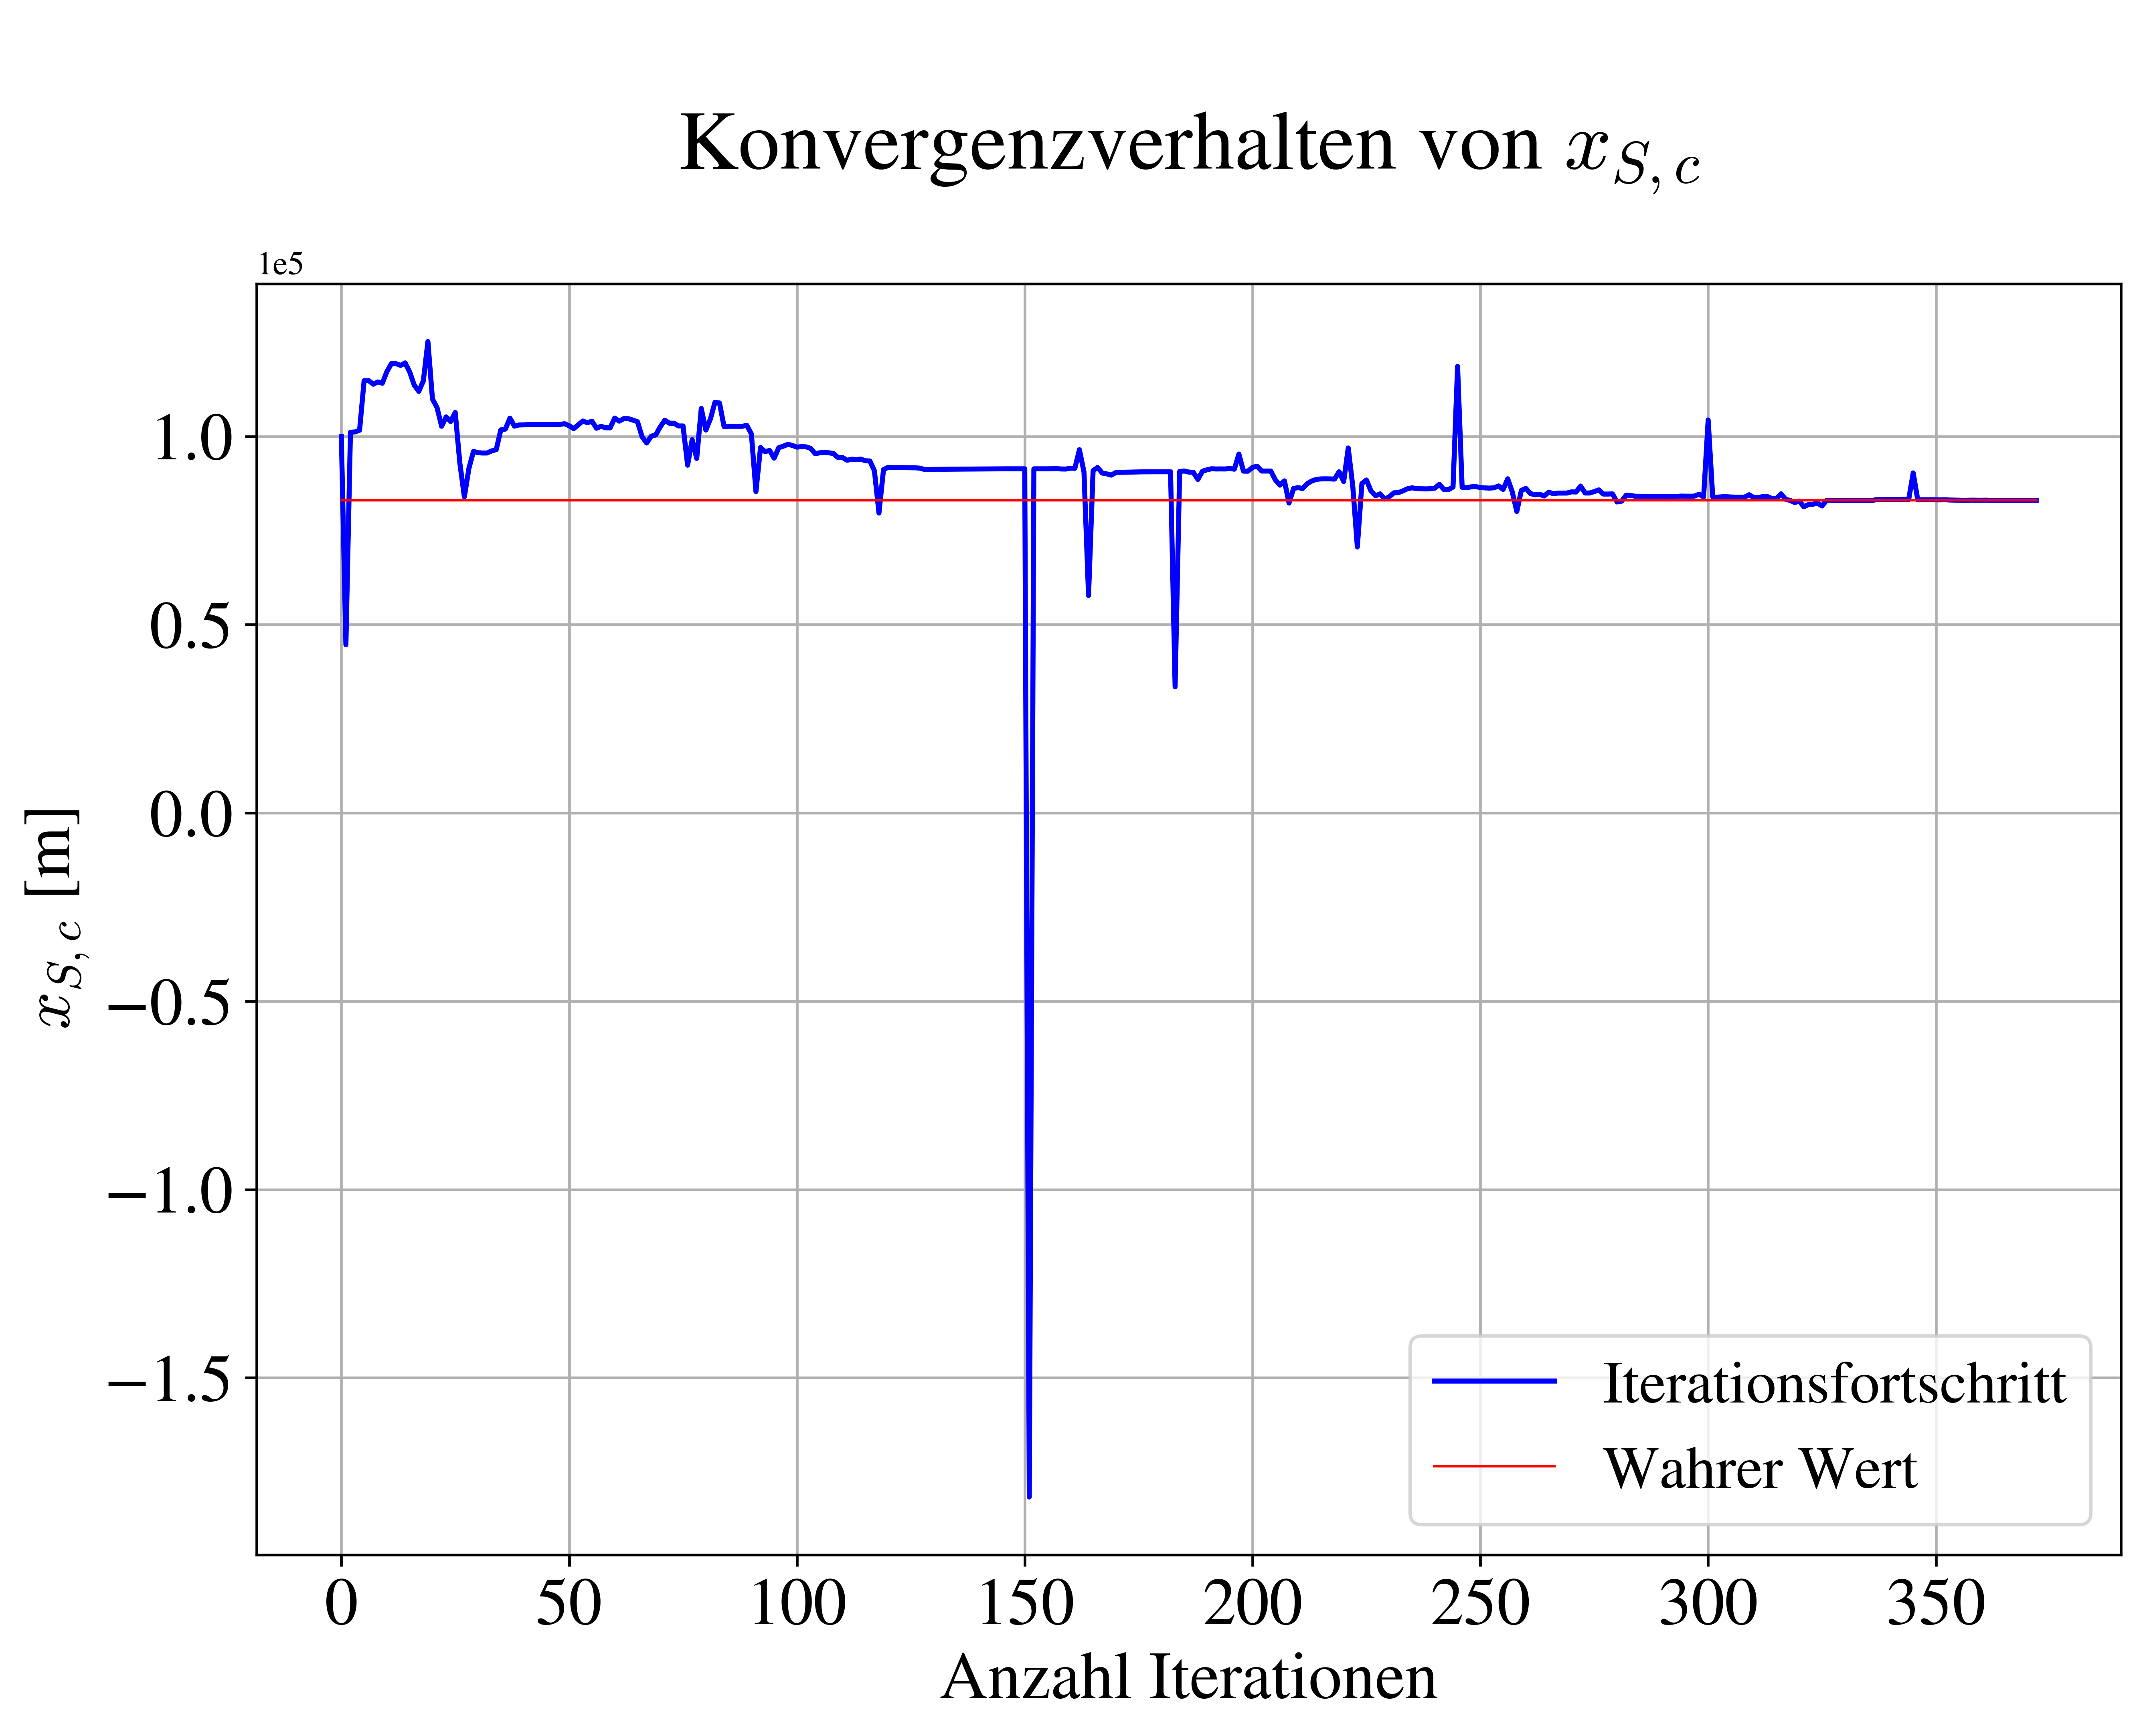
\includegraphics[width=\textwidth]{figures/conv_xp.png}
	\caption{Konvergenzverhalten der Koordinate $x_{S,c}$.}
	\label{fig:konvverh1xp}
	\end{subfigure}
	\hfill
	\begin{subfigure}[t]{0.49\textwidth}
	\centering
	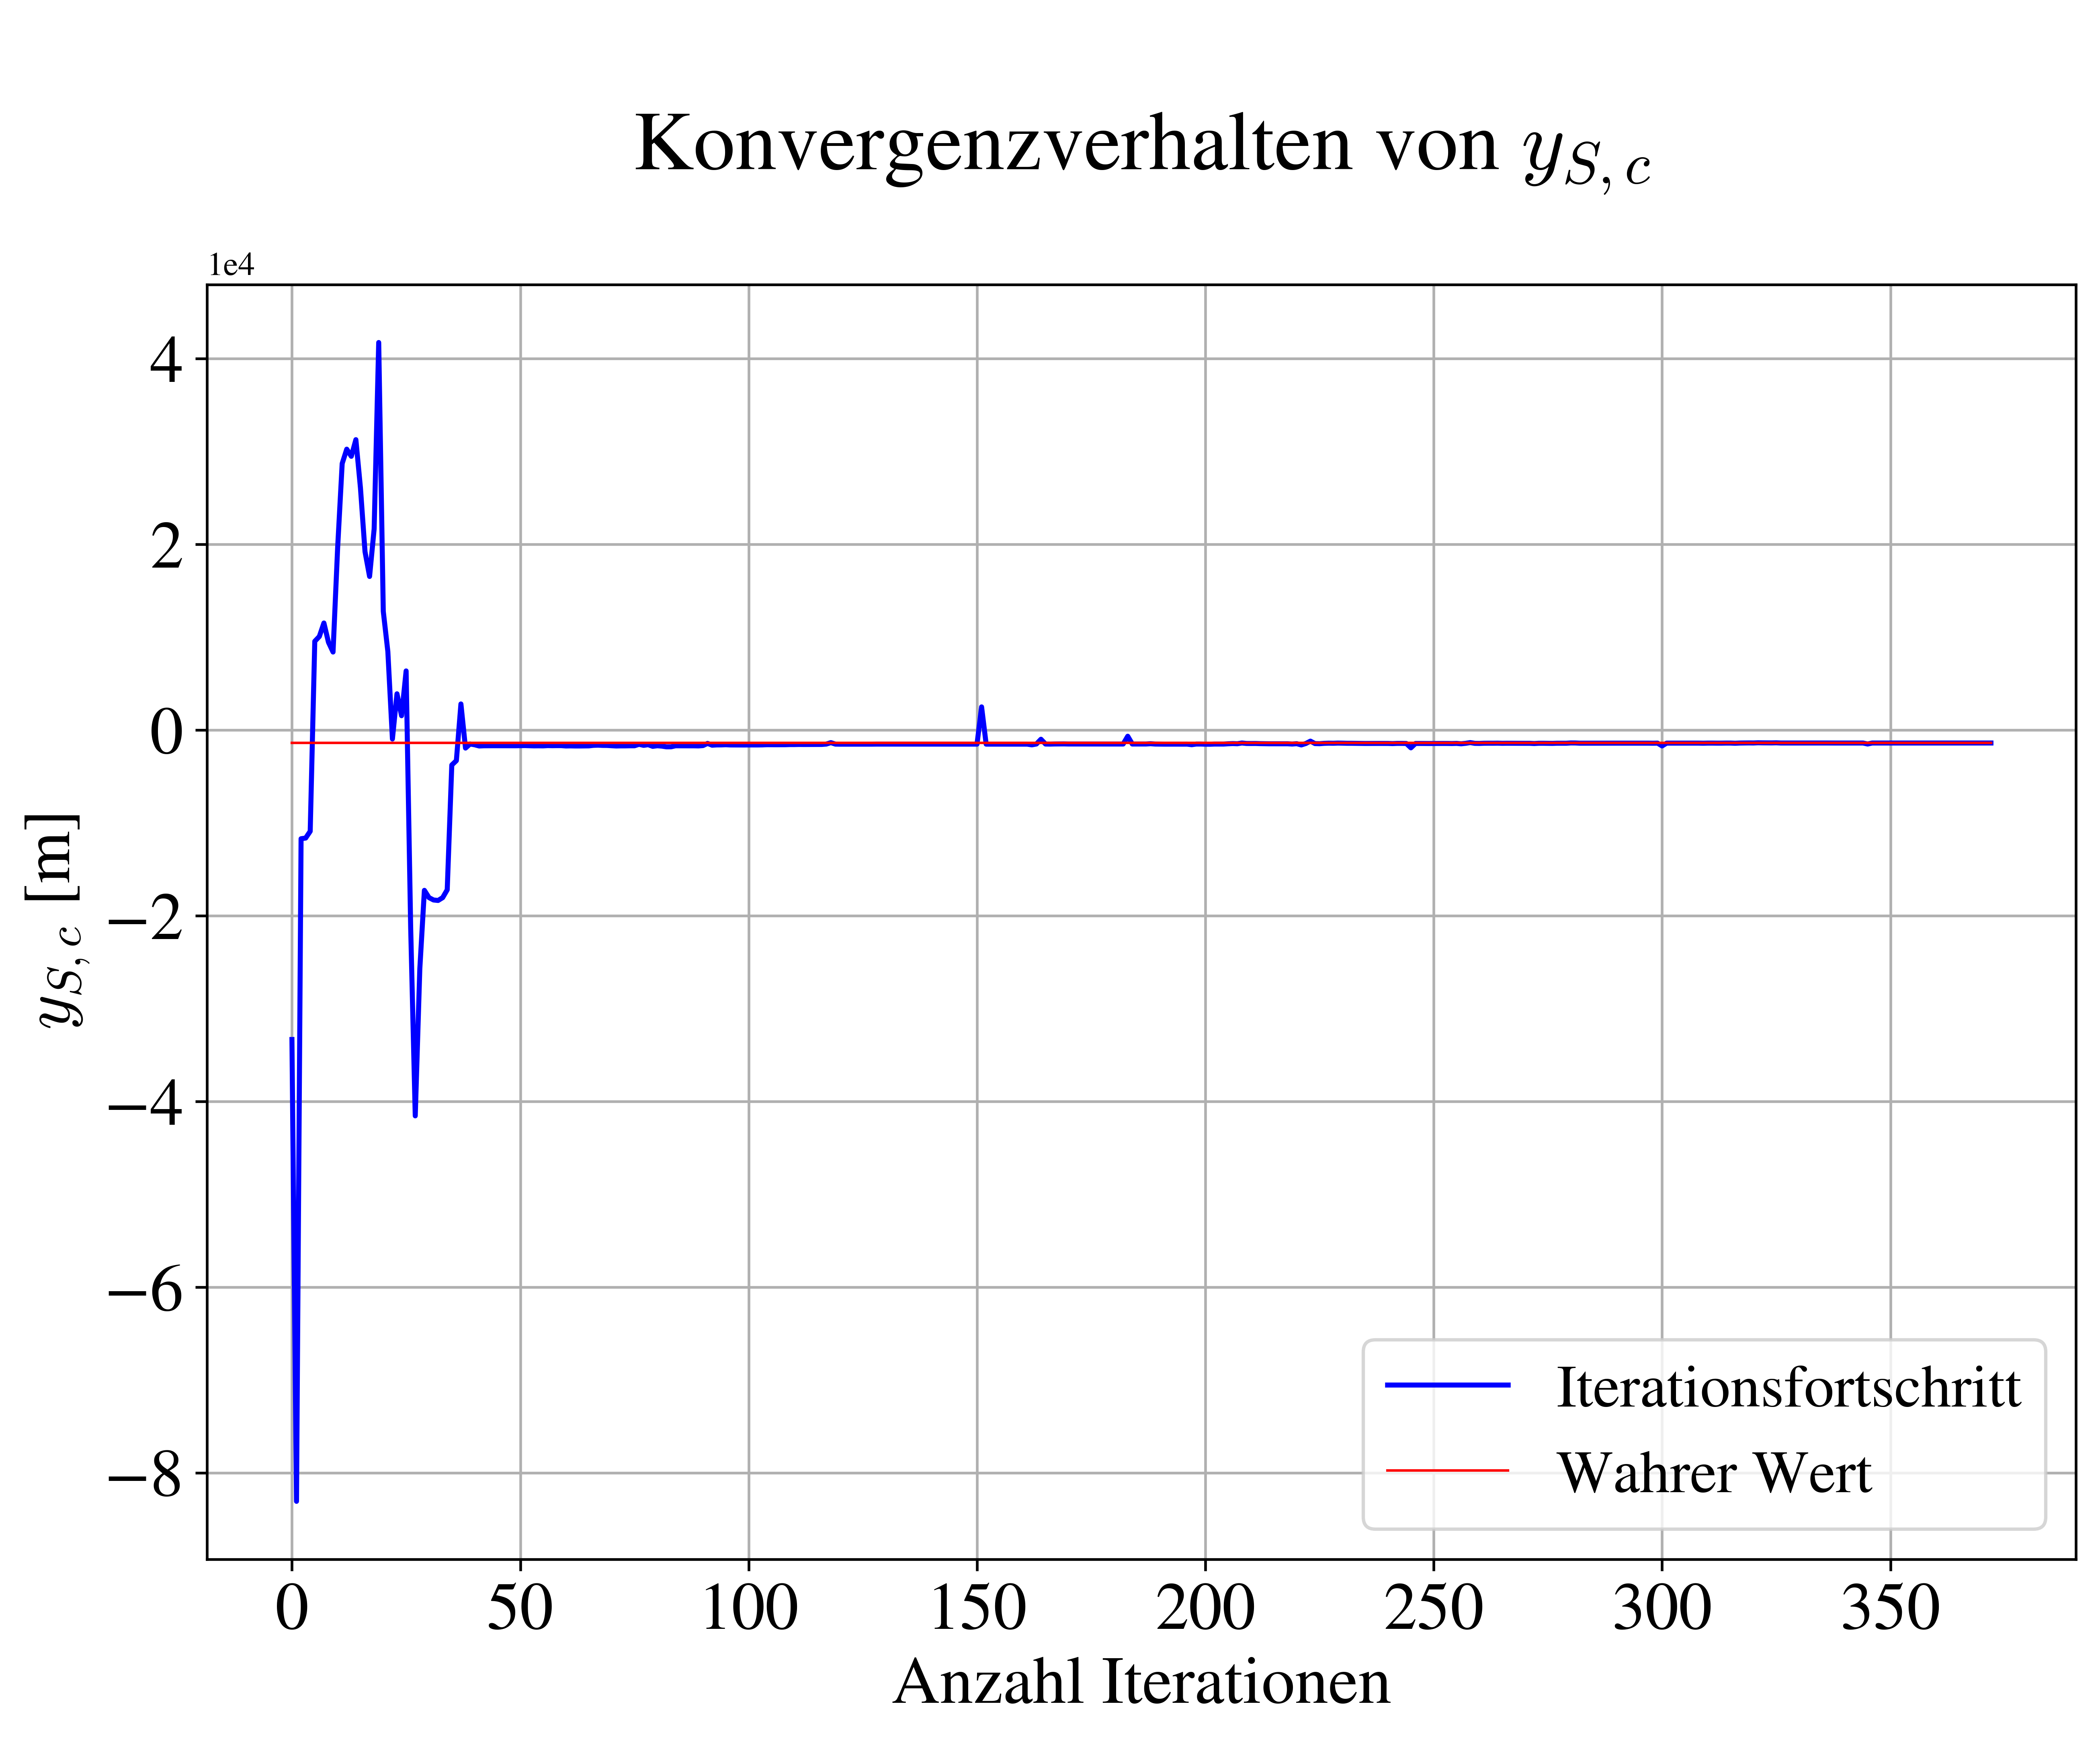
\includegraphics[width=\textwidth]{figures/conv_yp.png}
	\caption{Konvergenzverhalten der Koordinate $y_{S,c}$.}
	\label{fig:konvverh2yp}
	\end{subfigure}
\end{figure}
\begin{figure}[ht]\ContinuedFloat
	\centering
	\begin{subfigure}[t]{0.49\textwidth}
	\centering
	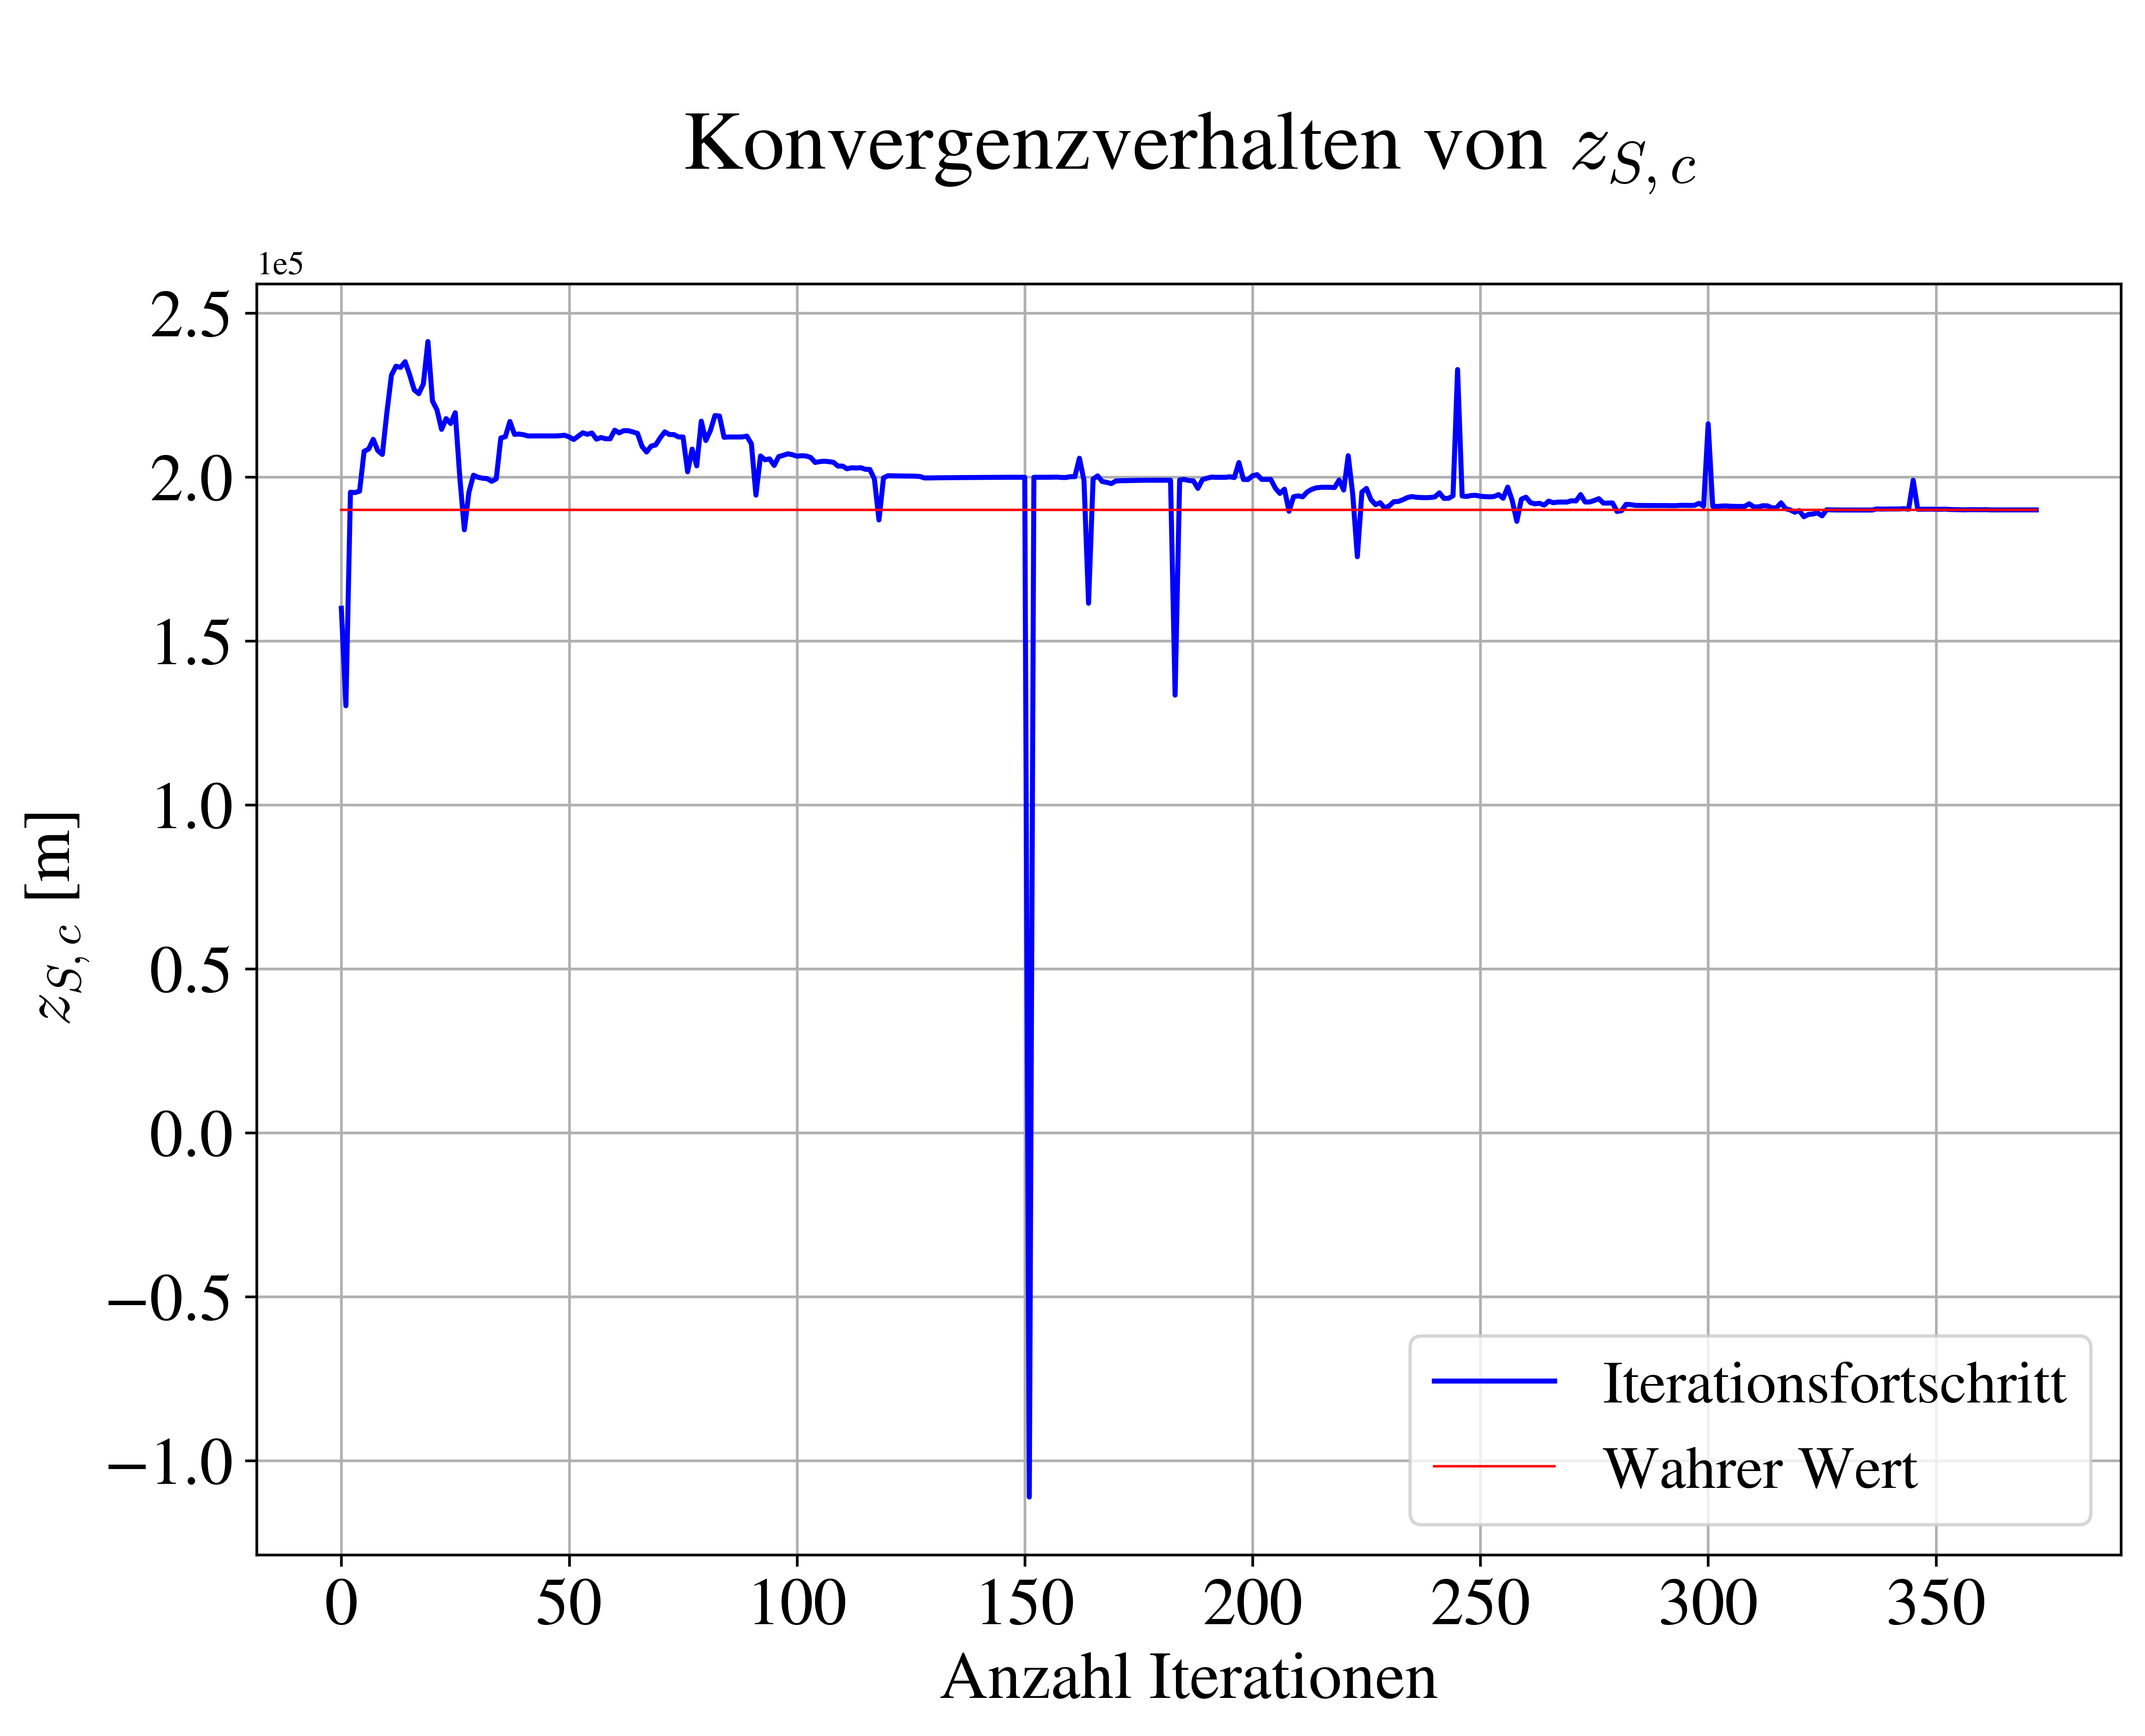
\includegraphics[width=\textwidth]{figures/conv_zp.png}
	\caption{Konvergenzverhalten der Koordinate $z_{S,c}$.}
	\label{fig:konvverh3zp}
	\end{subfigure}
	\hfill
	\begin{subfigure}[t]{0.49\textwidth}
	\centering
	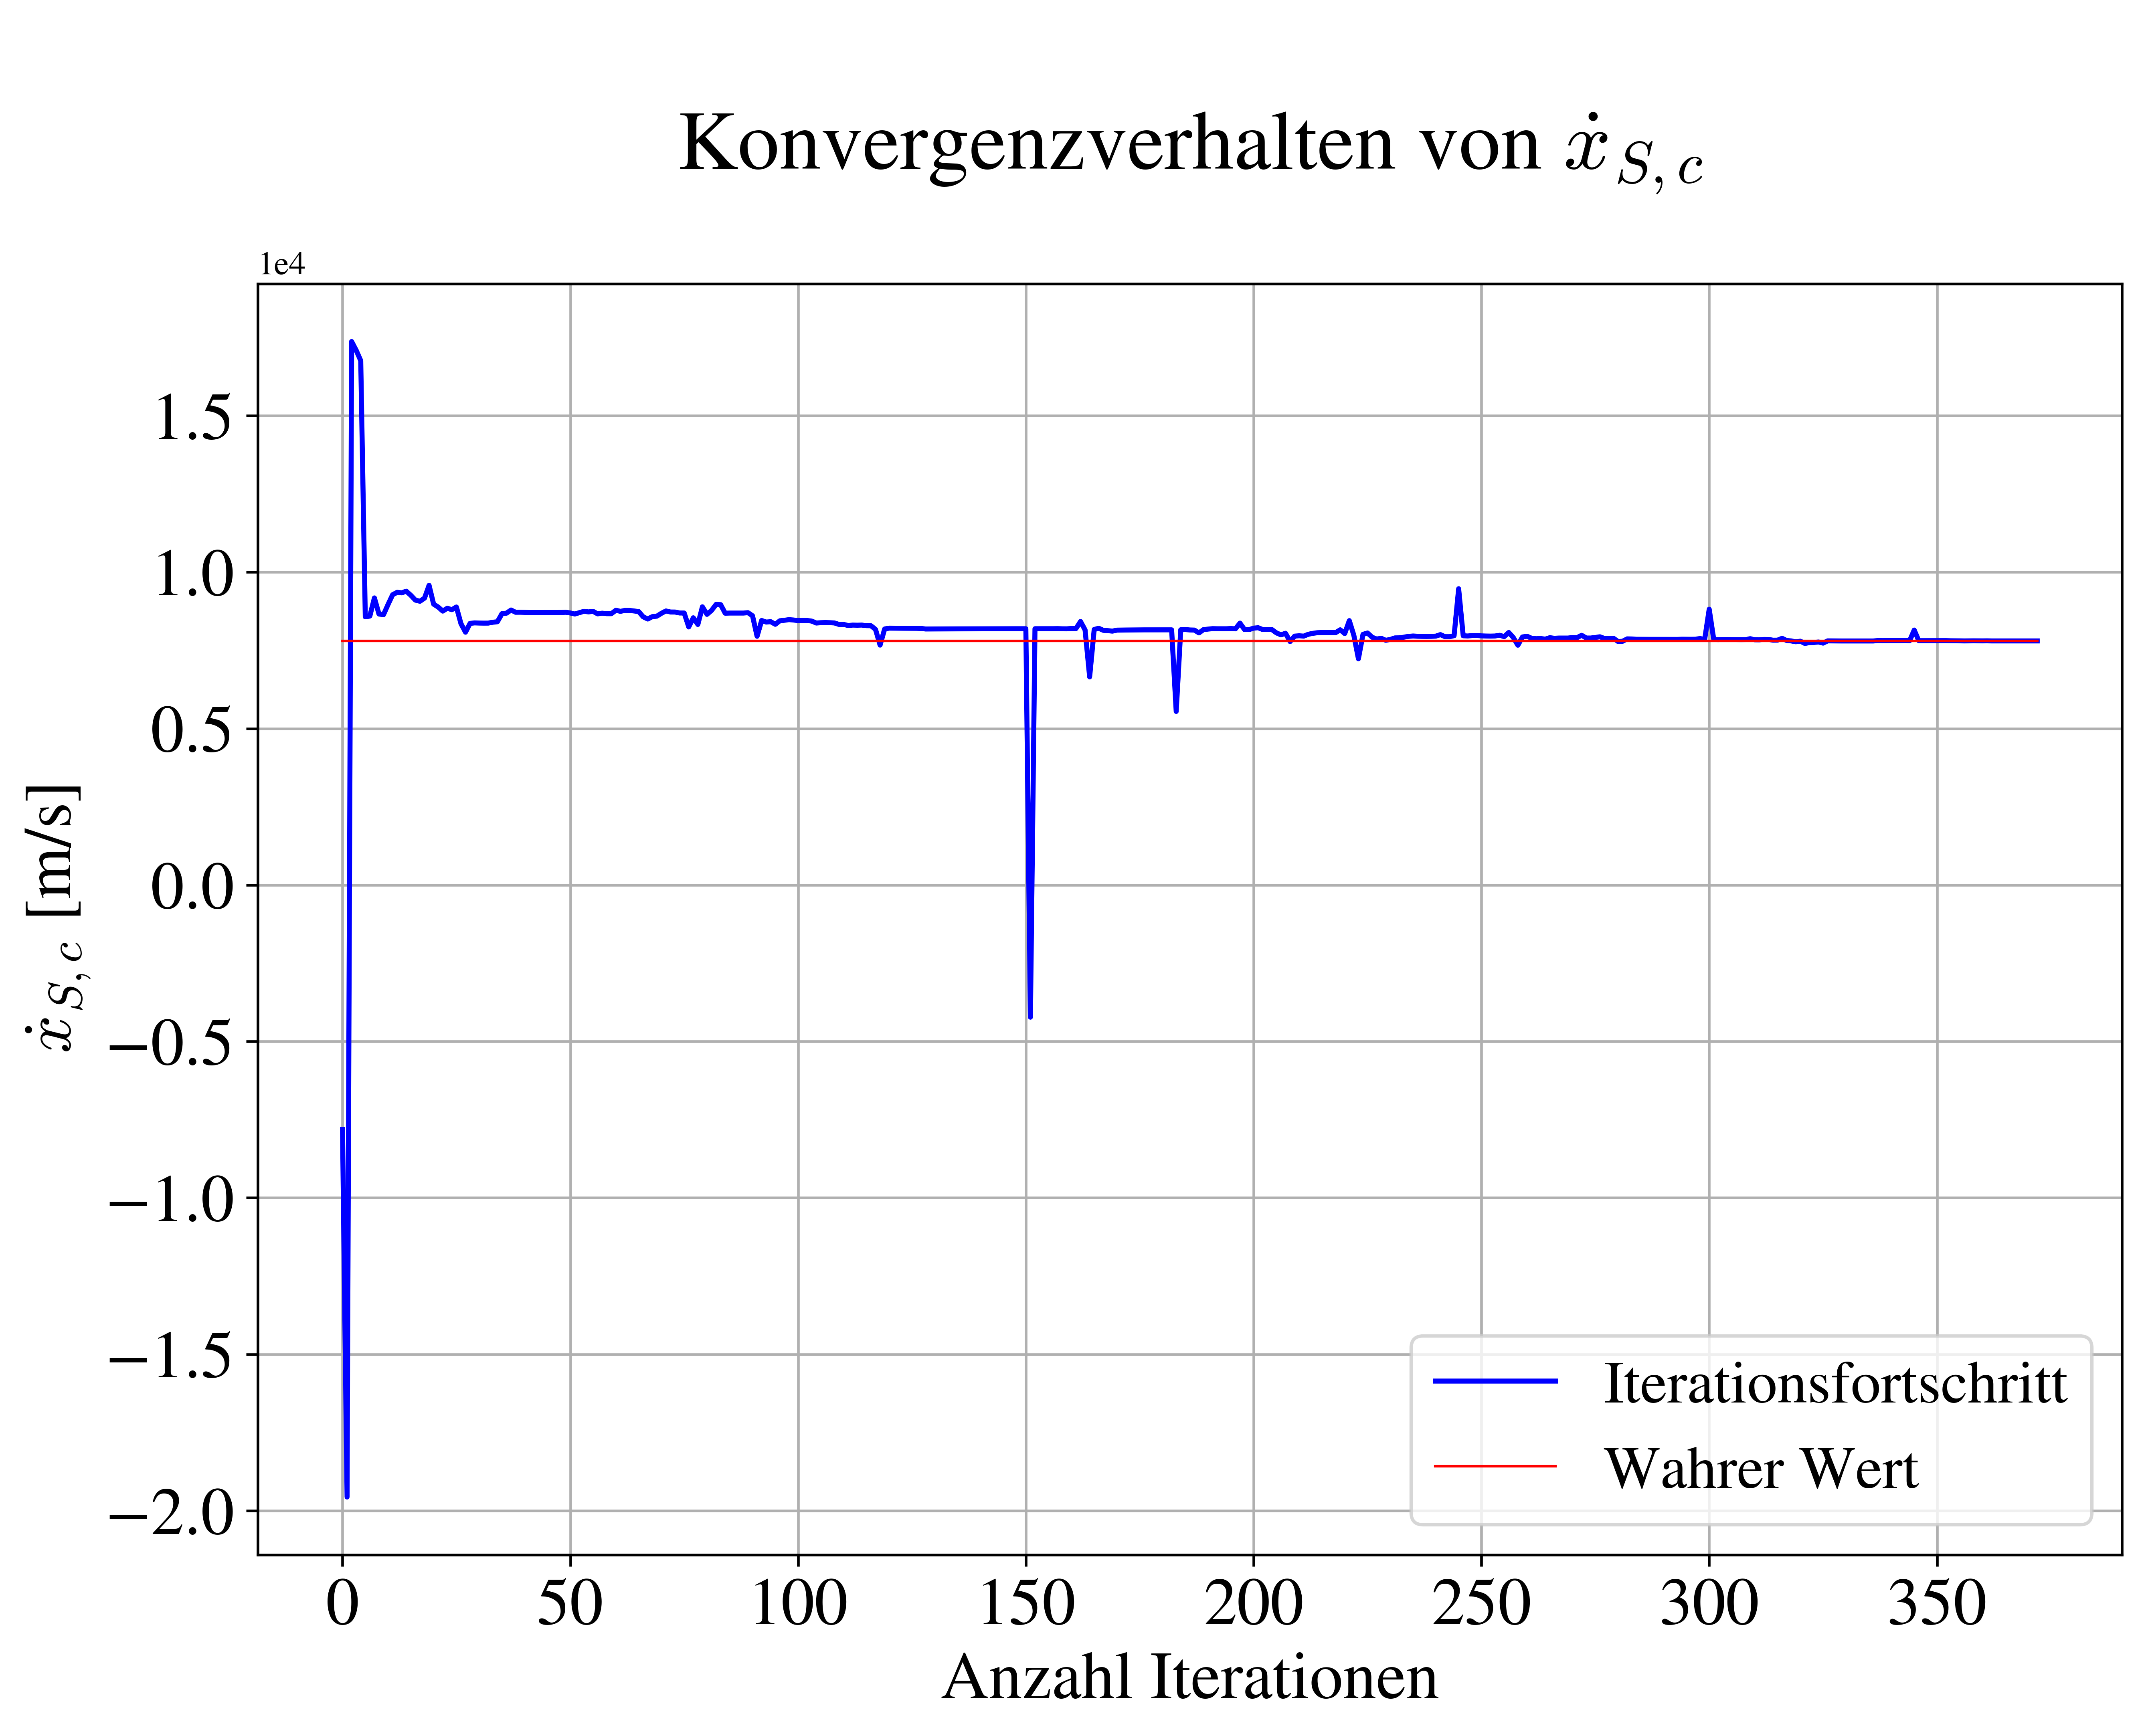
\includegraphics[width=\textwidth]{figures/conv_xv.png}
	\caption{Konvergenzverhalten der Koordinate $\dot{x}_{S,c}$.}
	\label{fig:konvverh4xv}
	\end{subfigure}
\end{figure}
\begin{figure}[ht]\ContinuedFloat
	\begin{subfigure}[t]{0.49\textwidth}
	\centering
	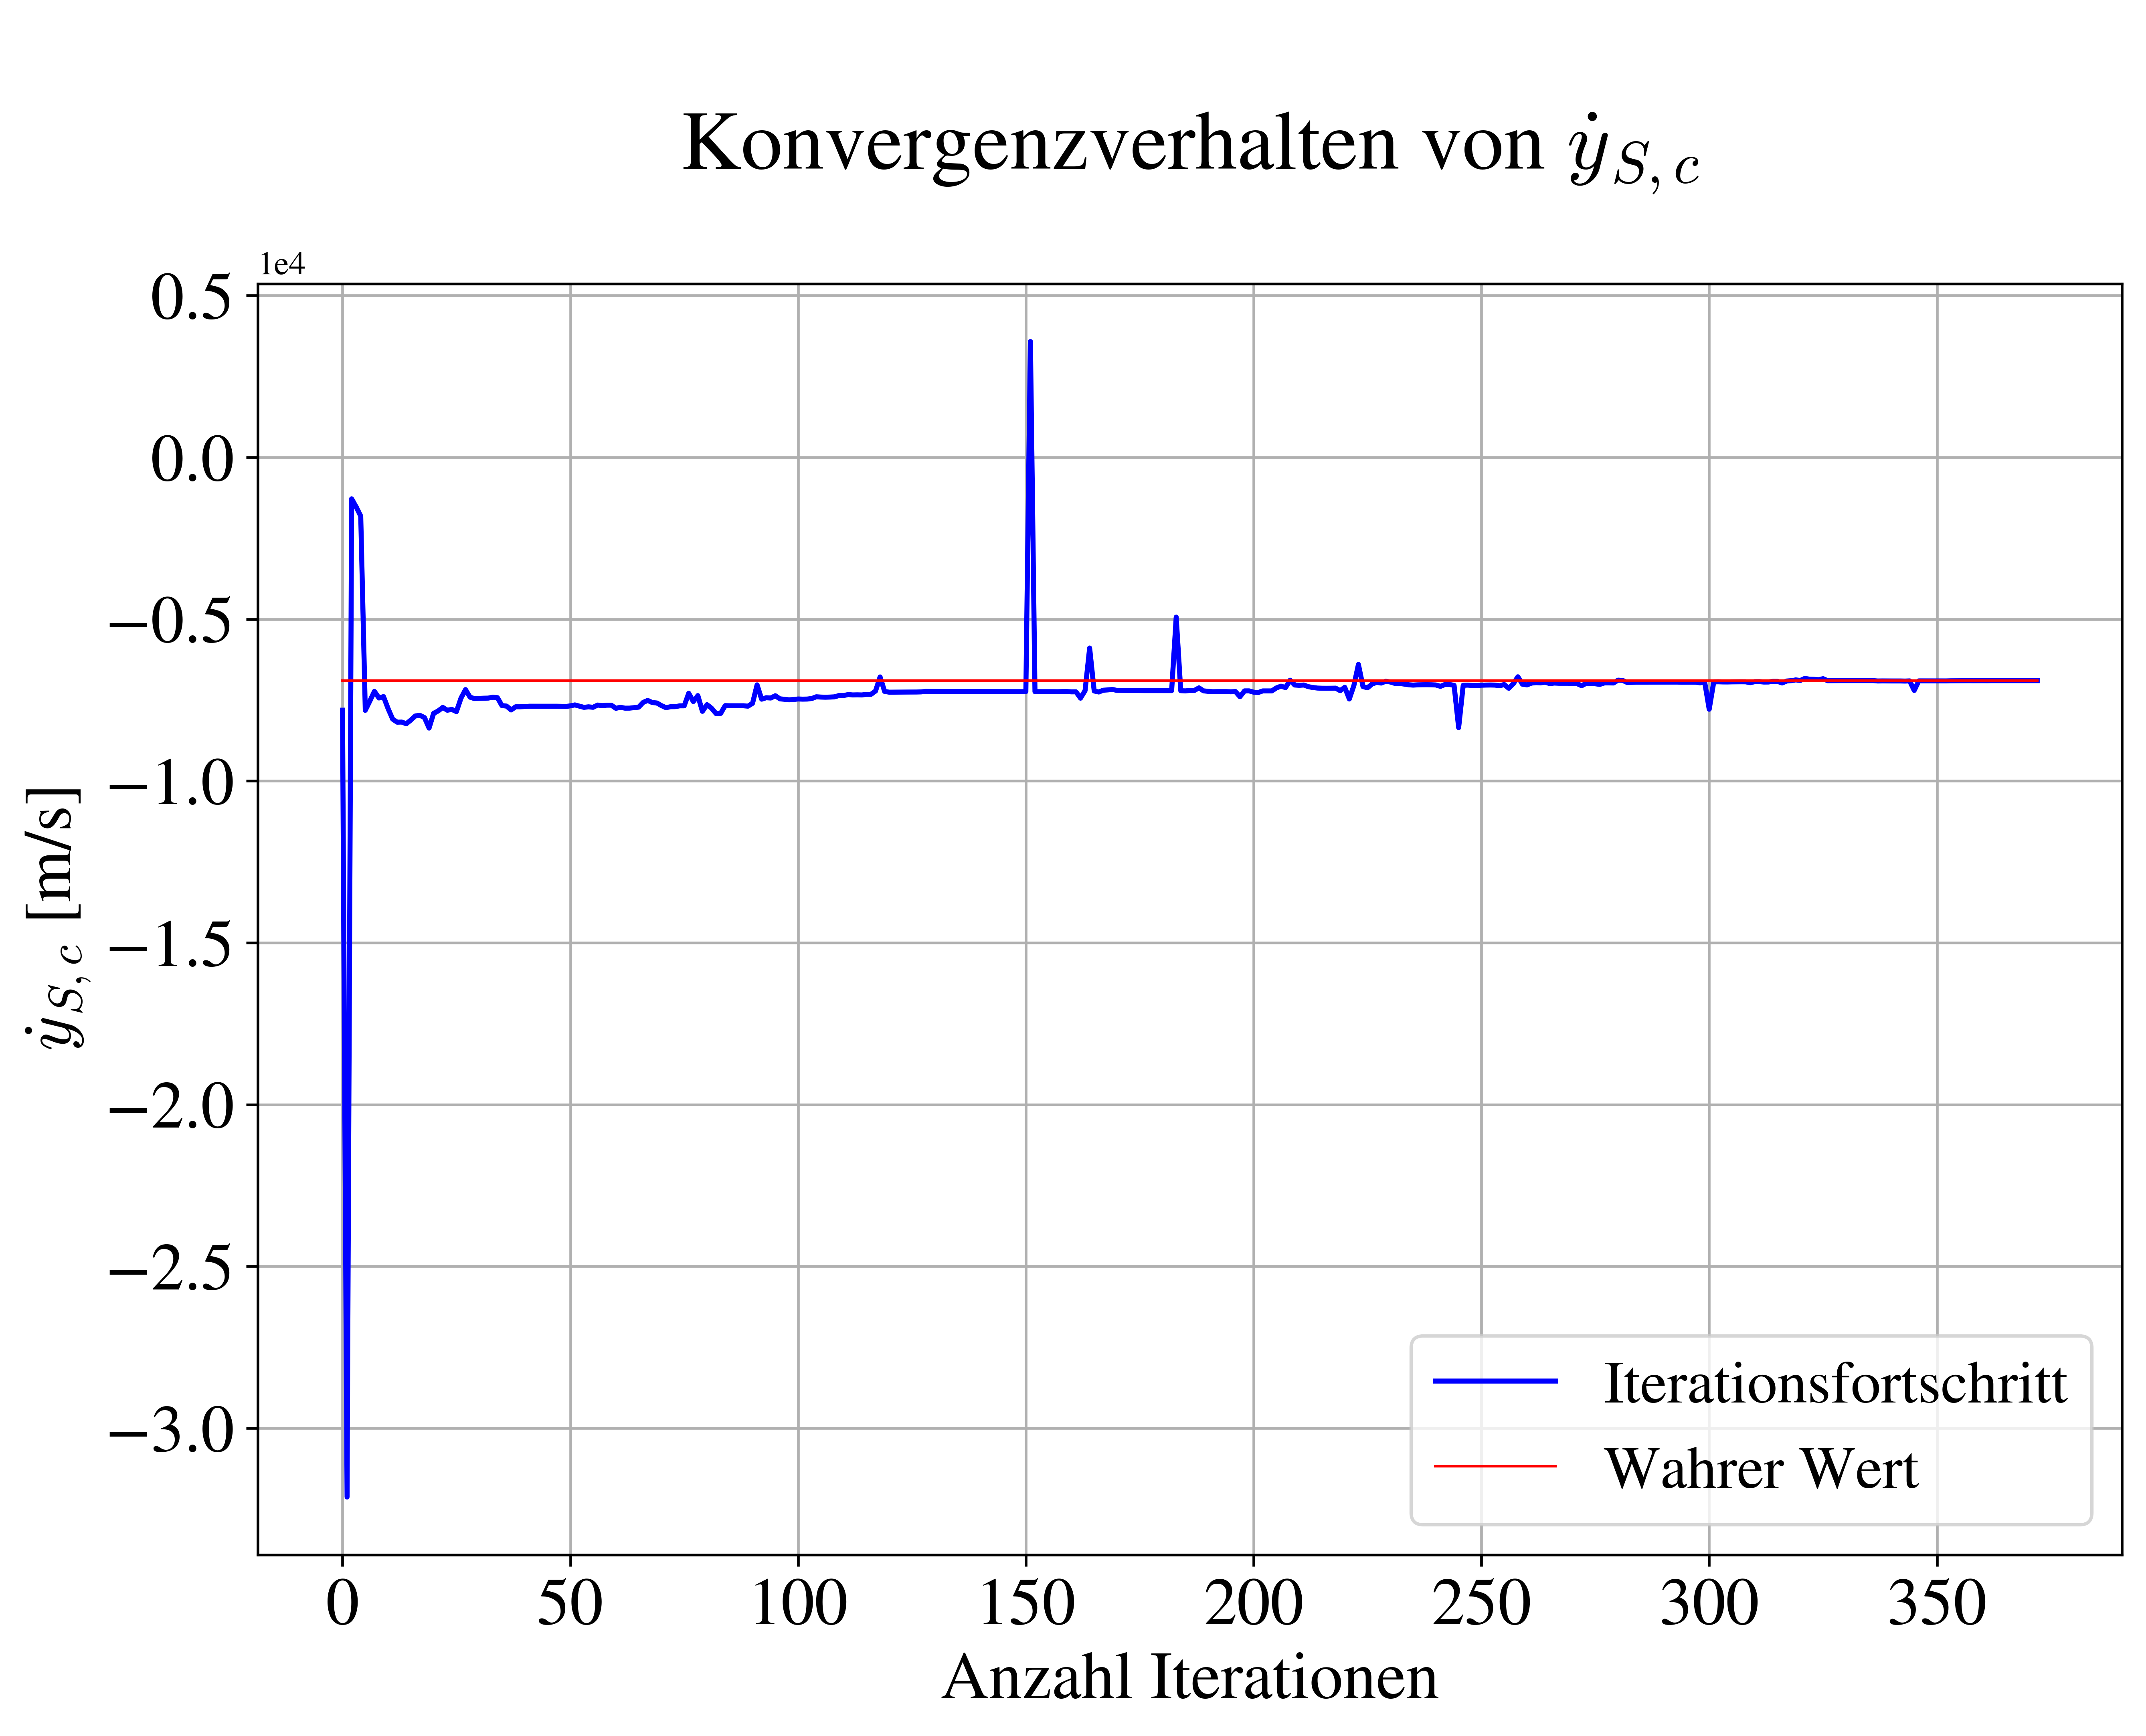
\includegraphics[width=\textwidth]{figures/conv_yv.png}
	\caption{Konvergenzverhalten der Koordinate $\dot{y}_{S,c}$.}
	\label{fig:konvverh5yv}
	\end{subfigure}
	\hfill
	\begin{subfigure}[t]{0.49\textwidth}
	\centering
	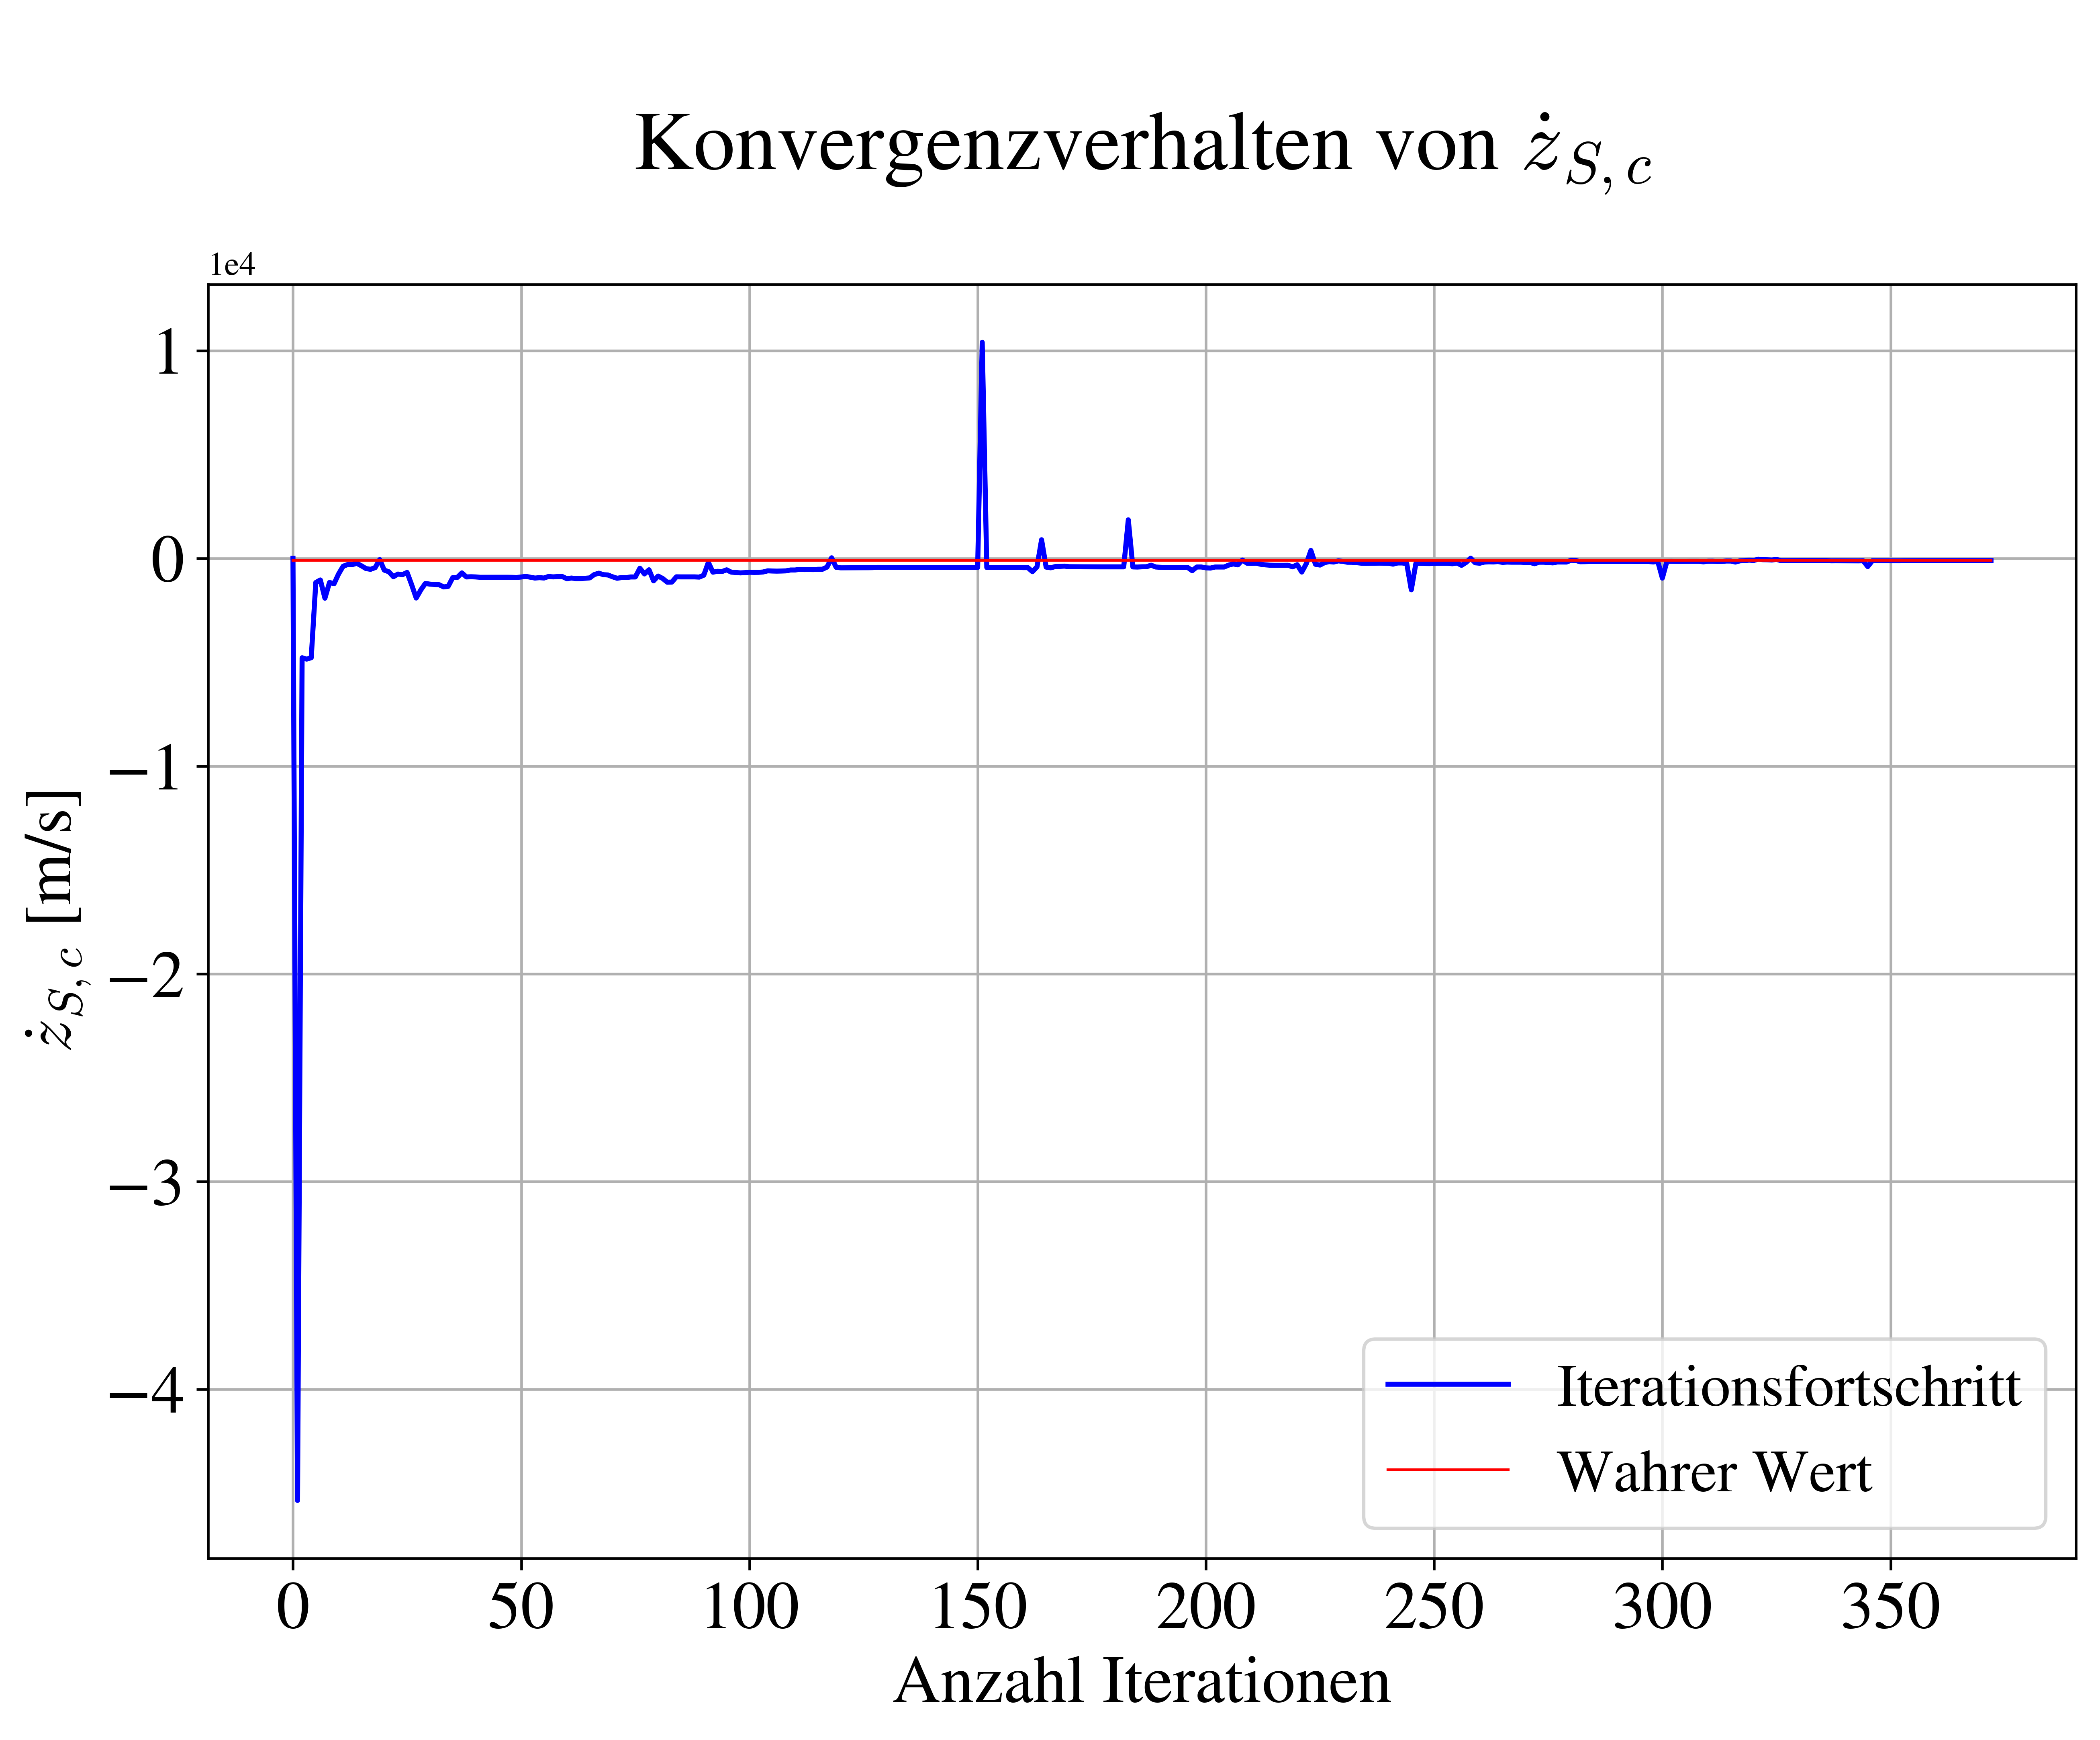
\includegraphics[width=\textwidth]{figures/conv_zv.png}
	\caption{Konvergenzverhalten der Koordinate $\dot{z}_{S,c}$.}
	\label{fig:konvverh6zv}
	\end{subfigure}
\cprotect\caption{Konvergenzverhalten des im Programm \verb|numsolver.py| implementierten Newton-Iterationsverfahrens bei der initialen Lösungsfindung.}
\end{figure}
\FloatBarrier

Eine Gegenüberstellung der benutzten Testkoordinate $\rho_{t13}$ und der Abweichung $\Delta \rho_{c13}$ für die im initialen Iterationsverfahren berechnete Koordinate $\rho_{c13}$ ist in der nachfolgenden Tabelle \ref{tab:testconfig6} zu finden.

\begin{table}[ht]
\renewcommand{\arraystretch}{1.1}
\centering
\begin{tabular}{|c|c|c|c|c|c|c|}
\cline{2-7}
\multicolumn{1}{c|}{} & \multicolumn{3}{c|}{Position ($\si{\meter}$)} & \multicolumn{3}{c|}{Geschwindigkeit ($\si{\meter\per\second}$)} \\
\cline{2-7}\hline
$\rho_{t13}$ & $\num{8.3e4}$ & $\num{-1.4e3}$ & $\num{1.9e5}$ & $\num{7.8e3} $ & $\num{-6.9e3}$ & $\num{-1.1e2}$ \\
$\Delta \rho_{c13}$ & 0.037 & 0.001 & 0.046 & 0.002 & 0.002 & 0.001 \\
\hline
\end{tabular}
\caption{Testkoordinaten $\rho_{t13}$ und Abweichung $\Delta \rho_{c13}$ des inital berechneten Lösungsvektors zu der Testkoordinate. Die Ergebnis $\Delta \rho_{c13}=(|x_{S,t13}-x_{S,c13}|,|y_{S,t13}-y_{S,c13}|,|z_{S,t13}-z_{S,c13}|,|\dot{x}_{S,t13}-\dot{x}_{S,c13}|,|\dot{y}_{S,t13}-\dot{y}_{S,c13}|,|\dot{z}_{S,t13}-\dot{z}_{S,c13}|)$ ist auf drei Nachkommastellen gerundet.}
\label{tab:testconfig6}
\end{table}

Betrachtet man das in den Abbildungen \ref{fig:konvverh1xp} bis \ref{fig:konvverh6zv} dargestellte Konvergenzverhalten des initialen Iterationsverfahrens, so fällt auf, dass das Verfahren relativ langsam gegen eine Nullstelle von $F(\rho)
= 0$ konvergiert - über 350 Iterationsschritte sind hierfür nötig. Das liegt vermutlich daran, dass die Funktion $F(\rho)$ in der Nähe einer Lösung von $F(\rho) = 0$ hochgradig nichtlinear ist und deshalb vergleichsweise viele Iterationsschritte notwendig sind, um in den Linearitätsbereich der Funktion $F(\rho)$ um eine Nullstelle $\tilde{\rho}: F(\tilde{\rho}) = 0$ zu gelangen. Die Grafiken wurden erzeugt, indem für die initiale Iteration das Broyden-Verfahren des Python-Moduls \verb|scipy.optimize.root| verwendet wurde, da dieses über eine Callback-Möglichkeit verfügt. Das heisst, dass für jeden Iterationsschritt der entsprechend iterierte Lösungsvektor abgefragt werden kann. Normalerweise wird aber im Python-Modul \verb|scipy.optimize.root| eine Modifikation der Powell-Hybrid-Methode verwendet, welche in der Regel schneller konvergiert als das Broyden-Verfahren, jedoch über keine Callback-Möglichkeit verfügt. Das Broyden-Verfahren ist ein Quasi-Newton-Verfahren, basiert also auf dem in Abschnitt \ref{sec:globloesnonlinear} geschilderten Verfahren und verfügt gemäss der SciPy-Community über Backtracking und Line Searching \cite{SciPyDoc.20.05.2022}.


\subsubsection{Generelle Erkenntnisse zum numerischen Lösungsverfahren}
Eine Betrachtung der Ergebnisse der Routine \verb|numsolver.py| für verschiedene Testkonfigurationen liefert die Erkenntnis, dass generell genauere Ergebnisse erzielt werden, je näher die Testkonfiguration räumlich dem Ursprung des Koordinatensystems ist. Ferner gewinnt man die Erkenntnis, dass \verb|numsolver.py| für eine verdoppelte Basislinie $a$ der Messgeometrie generell die besseren Ergebnisse liefert als für eine halbierte Basislinie. Diese Beobachtungen können dadurch plausibilisiert werden, dass die Unterschiede in den gemessenen Dopplerdaten an den verschiedenen Empfängerorten desto grösser werden, je näher die Testkonfiguration räumlich dem Ursprung des Koordinatensystems ist. Eine grössere Unterschiedlichkeit in den Dopplerdaten liefert erwartungsgemäss eine bessere Determination einer Lösung und folglich bessere und eindeutigere Konvergenzeigenschaften des Newton-Verfahrens - mutmasslich insbesondere dann, wenn eine realistische Situation mit Messunsicherheiten und Messrauschen auf den Dopplersignalen vorliegt. Wie bereits erwähnt, wird die Lösung des Gleichungssystems \eqref{eq:GlLoesShames} in der vorliegenden Arbeit idealisiert durchgeführt, das heisst ohne Messrauschen und Messunsicherheiten auf den Dopplersignalen. 

Dass die Routine \verb|numsolver.py| in den seltensten Fällen eine exakte Lösung des Gleichungssystems \eqref{eq:GlLoesShames} liefert, kann mehrere Gründe haben. Erstens hat die verwendeten Python-Funktion \verb|scipy.optimize.root| eine gewisse Toleranz ungleich null, die zur Termination des Lösungsverfahren unterschritten werden muss. Ferner kann zweitens der Lösungsraum eine sehr kuriose Geometrie aufweisen, sodass es in unmittelbarer Nähe einer globalen Nullstelle von \eqref{eq:GlLoesShames} viele lokale Nullstellen geben kann. Als dritte Ursache der Ungenauigkeit kann das Lösungsverfahren \verb|scipy.optimize.root| in einer solchen lokalen Nullstelle landen, wenn der Startwert des Lösungsverfahren nicht nahe genug bei einer globalen Nullstelle gewählt wird. Zu guter Letzt weisen viertens Computer eine begrenzte Maschinengenauigkeit auf, dies kann bei sehr genauen Berechnungen eine Rolle spielen - in der hier vorliegenden Anwendung scheint dies aber unerheblich zu sein, da in einigen Fällen ungeachtet der Maschinengenauigkeit exakte\footnote{Exakt im Sinne davon, dass die Lösungsroutine auf drei Nachkommastellen gerundet das exakte Resultat ausgibt - also gewissermassen die Testkoordinaten wieder zurückgibt, sodass $\rho_t = \rho_c$.} Resultate erzielt werden. Manche der obigen ungenauen Resultaten können verbessert werden, indem die Abtastungsfeinheiten \verb|div| der Funktionen \verb|solseeker(z_vel, div)|, \verb|refiner1(z_vel, sol, diff, div)| und/oder \verb|refiner2(sol, diff, div)| erhöht werden - das geht aber, wie oben erwähnt, einher mit einem starken Anstieg der Rechenzeit.

\newpage
\section{Fazit}
Die Methode 1 mit einem Sender um einem Empfänger scheint zwar zunächst attraktiv zu sein, ist jedoch aufgrund der erforderlichen speziellen Geometrie des Senders nicht anwendbar auf die bereits bestehenden Einrichtungen in Europa - nichtsdestotrotz liefert diese Methode, wie Richards zeigt, erstaunlich genaue Resultate für die Bahnelemente von Raumobjekten \cite[S.1732]{Richards.1961}. In der vorliegenden Arbeit wurde jedoch aufgrund des Fehlens passender Sendestationen von einer konkreten Simulation dieser Methode abgesehen. Eine in dieser Arbeit durchgeführte rudimentäre Simulation der Methode 2 mit einem Sender und sechs Empfängern zeigt, dass das theoretisch hergeleitete Verfahren prinzipiell auf die bestehenden Einrichtungen in Europa anwendbar ist und zumindest für Objekte im LEO plausible Resultate liefern kann - sofern die zugrunde liegenden Dopplerdaten nur mit vernachlässigbarem Messrauschen belegt sind. Ein grosser Vorteil der Methode 2 gegenüber der Methode 1 ist dadurch gegeben, dass zur vollständigen Bahnbestimmung eines Raumobjektes nur Dopplerdaten einer einzigen Epoche notwendig sind. Mit Dopplerdaten vieler Epochen kann daher bereits eine Bahnverbesserung vorgenommen werden - was vielversprechende Resultate liefern könnte. In einem weiteren Schritt könnte dies aufbauend auf der in vorliegender Arbeit durchgeführten Simulation untersucht und geprüft werden. Ferner bleibt eine Untersuchung des Einflusses von nicht vernachlässigbarem Messrauschen und nicht vernachlässigbaren Messunsicherheiten auf die Konvergenzeigenschaften des Lösungsverfahrens nach Methode 2 weiterführender Arbeit vorbehalten.

\newpage
\section{Anhang}
\subsection{Spezielle Relativitätstheorie}
\subsubsection{Notation}
Die Spezielle Relativitätstheorie (SR) kann mittels sogenannten Vierervektoren $x^\mu$ formuliert werden. Ein Vierervektor ist definiert durch \begin{equation}\label{defvierervektor}
x^\mu = (x^0 = ct,x^k) = (x^0,x^1,x^2,x^3) = (x^0, \vec{x}\,),
\end{equation} wobei $c$ die Lichtgeschwindigkeit und $t$ die Zeit in einem Inertialsystem bezeichnet. Griechische Buchstaben $(\mu, \nu, \dots)$ werden für die Komponenten von Vierervektoren verwendet, lateinische Buchstaben $(i,j,\dots)$ für gewöhnliche Vektoren des euklidischen Raumes.

Eine Matrix $A$ wird als $A_{\mu\nu}$ dargestellt, wobei die Einstein'sche Summenkonvention angewandt wird. Eine Summation ist also stets über zwei identische Indizes zu verstehen, wovon einer tiefliegend und der andere hochliegend sein muss. Beispielsweise kann die Multiplikation einer $n\times m$-Matrix $A$ mit einem $n\times 1$-Vektor $v$ durch \begin{equation}
w = Av \quad \Leftrightarrow \quad w^\mu =\sum_{\nu = 1}^{m}A^\mu_{\ \nu} v^\nu \equiv A^\mu_{\ \nu} v^\nu
\end{equation} dargestellt werden, wobei \begin{enumerate}
\item die Summation immer über zwei gleiche Indizes läuft, von denen einer tief- und der andere hochgestellt ist,
\item $(A^\mu_{\ \nu})^T = (A^\nu_{\ \mu})$ gilt,
\item $(A^\mu_{\ \nu})^{-1} = (A_\mu^{\ \nu})$ gilt, sowie
\item Zeilennummern oben positioniert sind und Spaltennummern unten stehen.
\end{enumerate}

\subsubsection{Grundlagen}
Ein Inertialsystem ist ein Bezugssystem, welches sich relativ zum Fixsternhimmel mit keiner oder konstanter Geschwindigkeit bewegt, also relativ zum Fixsternhimmel unbeschleunigt ist. Das Relativitätsprinzip von Galilei besagt nach Torsten Fliessbach, dass \begin{enumerate*}
\renewcommand{\theenumi}{(G\arabic{enumi})}
\renewcommand\labelenumi{\theenumi}\item \label{Galileo1} alle Inertialsysteme gleichwertig\footnote{Das heisst, in allen Inertialsystemen gelten dieselben physikalischen Gesetzmässigkeiten.} sind und \item \label{Galileo2} die Newton'schen Axiome in allen Inertialsystemen gelten \cite[S.333]{Fliebach.1996}.
\end{enumerate*} Das Relativitätsprinzip von Einstein hingegen besagt gemäss Fliessbach, dass \begin{enumerate*}
\renewcommand{\theenumi}{(E\arabic{enumi})}
\renewcommand\labelenumi{\theenumi}\item \label{Einstein1} alle Inertialsysteme gleichwertig sind und \item \label{Einstein2} die Lichtgeschwindigkeit in allen Inertialsystemen isotrop konstant und gleich $c$ ist \cite[S.335]{Fliebach.1996}.
\end{enumerate*}

Die beobachtbaren Eigenschaften des Lichts sind nicht mit dem Galilei'schen Relativitätsprinzip \ref{Galileo1} und \ref{Galileo2} kompatibel, wohl aber mit dem Einstein'schen Relativitätsprinzip \ref{Einstein1} und \ref{Einstein2}. Matthias Blau gibt eine Möglichkeit an, die korrekte Transformationsvorschrift einer physikalischen Entität von einem Inertialsystem in ein anderes Inertialsystem zu finden, nämlich die Invarianz des Wellenoperators \begin{equation}
\Box = -\frac{1}{c^2}\frac{\partial^2}{\partial t^2} + \Delta = \eta^{\mu\nu}\partial_\mu\partial_\nu
\end{equation} unter der Transformation $x\mu \rightarrow \bar{x}^\mu$ zu fordern, wobei $\Delta = \vec{\nabla}^2$ der Laplace-Operator ist \cite[S.7]{Blau.2021}. Da Licht durch die Wellengleichung - die mittels des Wellenoperators $\Box$ ausgedrückt werden kann - beschrieben wird, ist dies unter einer Betrachtung von Prinzip \ref{Einstein2} eine plausible Forderung. Diese geforderte Invarianz führt als Transformationsvorschrift von physikalischen Entitäten zu den Poincaré-Transformationen, beziehungsweise zu den Lorentz-Transformationen.

\subsubsection{Minkowski-Raum}
In Analogie zum normalen, euklidischen Raum, ist der Minkowski-Raum ein reeller Raum $\mathbb{R}^4$, ausgestattet mit der Minkowski-Metrik $d_M$. Die Minkowski-Metrik ist definiert durch \begin{equation}
d_M: \mathbb{R}^4 \times \mathbb{R}^4 \rightarrow \mathbb{R}, \quad (x^\mu,x^\nu) \mapsto \eta_{\mu\nu}x^\mu x^\nu,
\end{equation} wobei $\eta_{\mu\nu} = \mathrm{diag}(-1,+1,+1,+1)$ (\flqq mostly-plus\frqq\ Konvention) der Minkowski-Tensor mit $\eta_{\mu\nu}\eta^{\nu\kappa} = \delta_\mu^{\ \kappa}$ ist. Der Minkowski-Raum ist sodann als Tupel $(\mathbb{R}^4,d_M)$ gegeben.

Das Minkowski-Linienelement $\mathrm{d}s^2$ im Minkowski-Raum ist nach Blau durch \begin{equation}
\mathrm{d}s^2 = \eta_{\mu\nu}\,\mathrm{d}x^\mu\,\mathrm{d}x^\nu
\end{equation} gegeben \cite[S.14]{Blau.2021}.

Der Gradient $\partial_\mu$ im Raum der Vierervektoren ist ein sogenannter kovarianter Lorentz-Vektor. Es gilt gemäss obiger Notation \begin{equation}\label{diffoplower}
\partial_\mu = \frac{\partial}{\partial x^\mu} = \left(\frac{\partial}{\partial x^0},\frac{\partial}{\partial x^1},\frac{\partial}{\partial x^2},\frac{\partial}{\partial x^3} \right) = \left(\frac{1}{c}\frac{\partial}{\partial t}, \vec{\nabla}\right).
\end{equation} Für den entsprechenden kontravarianten Lorentz-Vektor $\partial^\mu$ gilt \begin{equation}\label{diffopupper}
\partial^\mu = \eta^{\mu\nu}\partial_\nu = \left(\frac{1}{c}\frac{\partial}{\partial t},-\vec{\nabla}\right).
\end{equation}

\subsubsection{Poincaré- und Lorentz-Transformationen}
Eine Transformationsvorschrift \begin{equation}
L:(\mathbb{R},d_M) \rightarrow (\mathbb{R},d_M), \quad x^\mu \mapsto \bar{x}^\mu = L^\mu_{\ \nu}x^\nu + b^\mu, \quad b_\mu = \text{const.} \in \mathbb{R}^4
\end{equation} ist nach Blau genau dann eine Poincaré-Transformation, wenn $L$ das Minkowski-Linienelement $\mathrm{d}s$ invariant lässt \cite[S.14]{Blau.2021}:
\begin{equation}
\eta_{\mu\nu}\bar{x}^\mu\bar{x}^\nu = \eta_{\mu\nu}x^\mu x^\nu \quad \Leftrightarrow \quad \eta_{\mu\nu} L^\mu_{\ \kappa}L^\nu_{\ \delta} = \eta_{\kappa \delta} \quad \Leftrightarrow \quad L^T\eta L = \eta.
\end{equation} Diese Transformationen beschreiben Transformationen zwischen Inertialsystemen von beliebigen, in Vierervektoren ausgedrückten physikalischen Entitäten. Die Invarianz des Minkowski-Linienelementes $\mathrm{d}s$ und die Invarianz des Wellenoperators $\Box$ sind gemäss Blau äquivalent \cite[S.14]{Blau.2021}.

Es seien zwei Intertialsysteme $\Sigma$ und $\bar{\Sigma}$ gegeben, wobei sich das Inertialsystem $\bar{\Sigma}$ relativ zu $\Sigma$ mit der Geschwindigkeit $\vec{v}=(v,0,0)$ bewege. Ziel ist es nun, eine Transformation zwischen den Inertialsystemen zu finden, welche die Einstein'schen Axiome \ref{Einstein1} und \ref{Einstein2} erfüllt. Die Erfüllung der Einstein'schen Axiome ist äquivalent mit der Invarianz des Wellenoperators $\Box$ unter den gesuchten Transformationen. Gemäss Ulrich Straumann ergeben sich aus den Einstein'schen Axiomen die folgenden Forderungen an die gesuchte Transformationsvorschrift \cite[S.9]{Straumann.2013}:
\begin{enumerate}
\item Aus dem Einstein'schen Axiom \ref{Einstein1} folgt, dass die gesuchten Transformationsgleichungen linear sein müssen, denn wenn es quadratische Terme in Ort $\vec{x}$ und Zeit $t$ geben würde, so würden Terme, welche Ableitungen nach Ort oder Zeit enthalten, noch von Ort und Zeit abhängig sein. Aufgrund der geforderten Gleichwertigkeit aller Inertialsysteme ist dies jedoch unzulässig - denn Gleichwertigkeit heisst Gleichförmigkeit derselben physikalischen Grundgesetze.
\item Aus dem Einstein'schen Axiom \ref{Einstein2} ergibt sich die Forderung der konstanten Lichtgeschwindigkeit und 
\item ferner die Bedingung, dass die gesuchte Transformationsvorschrift für $v \ll c$ in die Galileitransformation übergeht.
\end{enumerate}
Verwendet man die Notation $x^\mu = (ct,x^1,x^2,x^3)$ für Koordinaten im Inertialsystem $\Sigma$ und $\bar{x}^{\mu} = (c\bar{t},\bar{x}^{1},\bar{x}^{2},\bar{x}^{3})$ für Koordinaten im Inertialsystem $\bar{\Sigma}$, so ergibt sich aus der dritten Forderung die Bedingung \begin{equation}\label{eq:bedlor1}
(x^1)^2+(x^2)^2+(x^3)^2 = c^2 \cdot t^2 \quad \Leftrightarrow \quad (\bar{x}^{1})^2+(\bar{x}^{2})^2+(\bar{x}^{3})^2 = c\cdot \bar{t}^{\,2},
\end{equation} indem man Straumann folgend den Ort und die Position eines Lichtblitzes betrachtet, der sich Kugelförmig ausbreitet \cite[S.10]{Straumann.2013}. Aus der ersten und zweiten Bedingung ergibt sich der folgende Ansatz für die gesuchte Koordinatentransformation:
\begin{equation}
\bar{x}^\mu = \begin{pmatrix}
c \bar{t} \, \\ \bar{x}^1 \\ \bar{x}^2 \\ \bar{x}^3
\end{pmatrix} = \begin{pmatrix}
c (Bx^1 +  Dt) \\ A(x^1-vt) \\ x^2 \\ x^3
\end{pmatrix}, \quad A,B,D \in \mathbb{R}.
\end{equation} Setzt man diesen Ansatz in die Bedingungsgleichungen \eqref{eq:bedlor1} ein, ergeben sich die Koeffizienten $A$, $B$ und $D$ zu \begin{equation}
A = \gamma, \quad B = -\frac{\beta}{c}\gamma, \quad D = \gamma,\end{equation} wobei der Beta-Faktor und der Gamma-Faktor durch \begin{equation} \beta = \frac{v}{c}, \quad \gamma = \frac{1}{\sqrt{1-\beta^2}}
\end{equation} definiert sind. Damit lautet die Transformationgleichung \begin{equation}
\bar{x}^\mu = \begin{pmatrix}
c \bar{t}\, \\ \bar{x}^1 \\ \bar{x}^2 \\ \bar{x}^3
\end{pmatrix} = \begin{pmatrix}
-\beta \gamma x^1 + c \gamma t \\ \gamma (x^1-vt) \\ x^2 \\ x^3
\end{pmatrix} = \begin{pmatrix}
\gamma c t - \beta \gamma x^1 \\ -\beta \gamma c t + \gamma x^1 \\ x^2 \\ x^3
\end{pmatrix},
\end{equation} wobei $v = \beta c $ verwendet wurde. Die definierte Transformation $\bar{x}^\mu = L^\mu_{\ \nu} x^\nu$ kann mittels des (1,1)-Tensors $L^\mu_{\ \nu}$ - welcher im vorliegenden Fall in Matrixform geschrieben werden kann - ausgeschrieben durch \begin{equation}
\bar{x}^\mu = \begin{pmatrix}
c\bar{t} \\ \bar{x}^1 \\ \bar{x}^2 \\ \bar{x}^3
\end{pmatrix} = L^\mu_{\ \nu} x^\nu = \underbrace{\begin{pmatrix}
\gamma & -\beta\gamma & 0 & 0 \\
-\beta\gamma & \gamma & 0 & 0 \\
0 & 0 & 1 & 0 \\
0 & 0 & 0 & 1
\end{pmatrix}}_{= \, L^\mu_{\ \nu}}\underbrace{\begin{pmatrix}
ct \\ x^1 \\ x^2 \\ x^3
\end{pmatrix}}_{= \, x^\nu} = \begin{pmatrix}
\gamma ct - \beta\gamma x^1 \\ -\beta\gamma ct + \gamma x^1 \\ x^2 \\ x^3
\end{pmatrix}
\end{equation} repräsentiert werden. Es kann gezeigt werden, dass $L^\mu_{\ \nu}$ die Relation \begin{equation}
\eta_{\mu\nu} L^\mu_{\ \kappa}L^\nu_{\ \delta} = \eta_{\kappa \delta}
\end{equation} erfüllt, und somit eine Lorentz-Transformation sein muss. Mit der durch $L \doteq L^\mu_{\ \nu}$ definierten speziellen Lorentz-Transformation in den Koordinaten $(x^0=ct, x^1)$ kann nach Christoph Greub jede beliebige Transformation $\mathcal{T}$ zwischen zwei Inertialsystemen dargestellt werden, indem Rotationen $R$ in den Koordinaten $\vec{x} = (x^1,x^2,x^3)$, Translationen $T$ in den Koordinaten $x^\mu = (x^0=ct,x^1,x^2,x^3)$ und spezielle Lorentz-Transformationen $L$ in den Koordinaten $(x^0 = ct, x^1)$ hintereinander ausgeführt werden \cite[S.137-139]{Greub.2019}. Es gilt also für eine beliebige Transformation zwischen zwei Inertialsystemen die Definitionsgleichung \begin{equation}
\mathcal{T} = L \circ R \circ T \quad \Leftrightarrow \quad \bar{x}^\mu = \mathcal{T}(x^\mu) = (L\circ T \circ R)(x^\mu) = L(R(T(x^\mu))).
\end{equation}

\subsubsection{Eigenzeit und Eigenraum}
Es sei mit $x^\mu$ und $\bar{x}^\mu$ dieselbe Weltlinie eines massiven Teilchens in verschiedenen Inertialsystemen $\textrm{IS}$ und $\overline{\textrm{IS}}$ beschrieben. Im bewegten System $\overline{\textrm{IS}}$ nimmt das Differential des Vierervektors $\bar{x}^\mu$ die Form  $\mathrm{d}\bar{x}^\mu = (c\,\mathrm{d}\bar{t},0,0,0)$ an, somit schreibt sich folglich das Minkowski-Linienelement zu $\mathrm{d}\bar{s}^{\,2} = \eta_{\mu\nu}\,\mathrm{d}\bar{x}^\mu\,\mathrm{d}\bar{x}^\nu = -c^2\,\mathrm{d}\bar{t}^{\,2} \doteq -c^2\,\mathrm{d}\tau^2.$
Es gilt aufgrund der Invarianz unter Lorentz-Transformationen \begin{equation}
\mathrm{d}\bar{s} = \mathrm{d}s \quad \Leftrightarrow \quad -c^2\mathrm{d}\tau^2 = -c^2\mathrm{d}t^2 + (\mathrm{d}x^1)^2 + (\mathrm{d}x^2)^2 + (\mathrm{d}x^3)^2 = -c^2(\mathrm{d}t)^2 + (\mathrm{d}\vec{x}\,)^2.
\end{equation} Für ein Differential $(\mathrm{d}q)^n$ gilt stets die Schreibweise $\mathrm{d}q^n \equiv (\mathrm{d}q)^n, n \in \mathbb{N}$. Daraus ergibt sich mit \begin{equation}
\vec{v}\,(t) = \frac{\mathrm{d}\vec{x}\,(t)}{\mathrm{d}t} \quad \Rightarrow \quad \mathrm{d}\tau^2 = \mathrm{d}t^2-\frac{(\mathrm{d}\vec{x}\,)^{2}}{c^2} \quad \Leftrightarrow \quad \mathrm{d}\tau = \mathrm{d}t\,\sqrt{1-\frac{\vec{v}\,(t)^2}{c^2}} = \gamma(\vec{v}\,)^{-1}\mathrm{d}t,
\end{equation} wobei $\gamma(\vec{v}\,) = (1-\nicefrac{\vec{v}\,(t)^2}{c^2})^{-\nicefrac{1}{2}} = (1-\beta(\vec{v}\,)^2)^{-\nicefrac{1}{2}}$ der Gamma-Faktor ist. Das Integral \begin{equation}
\tau_{PQ} = \int\displaylimits_{P}^{Q} \, \mathrm{d}\tau = \int\displaylimits_{t_P}^{t_Q} \sqrt{1-\frac{\vec{v}\,(t)^2}{c^2}} \,\mathrm{d}t
\end{equation} heisst dann gemäss Blau Eigenzeit \cite[S.21]{Blau.2021}.

In analoger Weise nehme das Differential des Vierervektors $\bar{x}^\mu$ im bewegten System $\overline{\textrm{IS}}$ die Form $\mathrm{d}\bar{x}^\mu = (0,\mathrm{d}\bar{x}^1,\mathrm{d}\bar{x}^2,\mathrm{d}\bar{x}^3)$ an. Somit schreibt sich folglich das Minkowski-Linienelement zu $\mathrm{d}\bar{s}^{\,2} = \eta_{\mu\nu}\,\mathrm{d}\bar{x}^\mu\,\mathrm{d}\bar{x}^\nu = (\mathrm{d}\bar{x}^1)^2+(\mathrm{d}\bar{x}^2)^2+(\mathrm{d}\bar{x}^3)^2 = (\mathrm{d}\bar{\vec{x}}\,)^2$. Es gilt aufgrund der Invarianz unter Lorentz-Transformationen \begin{equation}
\mathrm{d}\bar{s} = \mathrm{d}s \quad \Leftrightarrow \quad (\mathrm{d}\bar{\vec{x}}\,)^2 = -c^2\mathrm{d}t^2 + (\mathrm{d}x^1)^2 + (\mathrm{d}x^2)^2 + (\mathrm{d}x^3)^2 = -c^2(\mathrm{d}t)^2 + (\mathrm{d}\vec{x}\,)^2.
\end{equation} Daraus ergibt sich mit \begin{equation}
\vec{v}\,(t) = \frac{\mathrm{d}\vec{x}\,(t)}{\mathrm{d}t} \quad \Rightarrow \quad \mathrm{d}\bar{s}^{\,2} = -c^2\,\mathrm{d}t^2+(\mathrm{d}\vec{x}\,)^2 \quad \Leftrightarrow \quad \mathrm{d}\bar{s} = \mathrm{d}t\,\sqrt{\vec{v}\,(t)^2-c^2}.
\end{equation} Das Integral \begin{equation}
s_{PQ} = \int\displaylimits_{P}^{Q} \, \mathrm{d}\bar{s} = \int\displaylimits_{t_P}^{t_Q}\,\mathrm{d}t\,\sqrt{\vec{v}\,(t)^2-c^2}
\end{equation} heisst dann Eigenraum.

\subsubsection{Viererposition, Vierergeschwindigkeit, Viererbeschleunigung und Viererimpuls}
Durch die Eigenzeit $\tau$ ist ein Lorentz-invarianter Zeitparameter gegeben, der sich deshalb zur Parametrisierung von Weltlinien $x^\mu(t)$ eignet. Die Viererposition ist gegeben durch \begin{equation}\label{viererposition}
x^\mu(t) \doteq (ct,\vec{x}\,(t)), \quad x_\mu x^\mu = \eta_{\mu\nu}x^\mu x^\nu = -ct^2 + \vec{x}^{\,2}.
\end{equation} Die Vierergeschwindigkeit $u^\mu(\tau)$ ist nach Blau durch die Parametrisierung $x^\mu(\tau)$ gemäss \begin{equation}\label{vierergeschwindigkeit}
u^\mu(\tau) \doteq \frac{\mathrm{d}x^\mu(\tau)}{\mathrm{d}\tau} = (\gamma(\vec{v}\,)c,\gamma(\vec{v}\,)\vec{v}\,), \quad u_\mu u^\mu = \eta_{\mu\nu}u^\mu u^\nu = -c^2
\end{equation} gegeben \cite[S.34]{Blau.2021}. Die Viererbeschleunigung $a^\mu(\tau)$ ergibt sich sodann durch \begin{equation}\label{viererbeschleunigung}
a^\mu(\tau) \doteq \frac{\mathrm{d}^2x^\mu(\tau)}{\mathrm{d}\tau^2}.
\end{equation} Der Viererimpuls $p^\mu(\tau)$ wird gemäss Blau definiert durch \begin{equation}\label{viererimpuls}
p^\mu(\tau) \doteq mu^\mu(\tau) = m\frac{\mathrm{d}x^\mu(\tau)}{\mathrm{d}\tau} = m(\gamma(\vec{v}\,)c,\gamma(\vec{v}\,)\vec{v}\,), \quad p_\mu p^\mu = m^2\eta_{\mu\nu}u^\mu u^\nu = -m^2c^2,
\end{equation} wobei der Viererimpuls auch zu \begin{equation}
p^\mu(\tau) = (E/c, \vec{p}\,)
\end{equation} geschrieben werden kann, da $mc^2\gamma(\vec{v}\,)$ die relativistische Energie eines massiven Teilchens ist \cite[S.36]{Blau.2021}. Durch das Skalarprodukt \begin{equation}
p_\mu p^\mu = m^2\eta_{\mu\nu}u^\mu u^\nu = -m^2c^2 = -\frac{E^2}{c^2} + \vec{p}^{\,2} \quad \Leftrightarrow \quad E^2 = \vec{p}^{\,2}c^2 + m^2c^4
\end{equation} ergibt sich die bekannte Energie-Impuls-Beziehung, welche auch die \flqq Massenschale\frqq\ genannt wird.

\subsection{Herleitung des Dopplereffektes}
\subsubsection{Relativistischer Dopplereffekt für elektromagnetische Wellen im Vakuum}
Zwecks einer Herleitung des relativistischen Dopplereffektes für elektromagnetische Wellenphänomene sei Abbildung \ref{fig:herlDopplerrel} betrachtet.
\begin{figure}[h]
\centering


\tikzset{every picture/.style={line width=0.75pt}} %set default line width to 0.75pt        

\begin{tikzpicture}[x=0.75pt,y=0.75pt,yscale=-1,xscale=1]
%uncomment if require: \path (0,300); %set diagram left start at 0, and has height of 300

%Straight Lines [id:da9602866414376943] 
\draw  [dash pattern={on 0.84pt off 2.51pt}]  (130,180) -- (130,133) ;
\draw [shift={(130,130)}, rotate = 90] [fill={rgb, 255:red, 0; green, 0; blue, 0 }  ][line width=0.08]  [draw opacity=0] (7.14,-3.43) -- (0,0) -- (7.14,3.43) -- cycle    ;
%Straight Lines [id:da5407545903064199] 
\draw  [dash pattern={on 0.84pt off 2.51pt}]  (130,180) -- (187,180) ;
\draw [shift={(190,180)}, rotate = 180] [fill={rgb, 255:red, 0; green, 0; blue, 0 }  ][line width=0.08]  [draw opacity=0] (7.14,-3.43) -- (0,0) -- (7.14,3.43) -- cycle    ;
%Straight Lines [id:da05851488618890177] 
\draw  [dash pattern={on 0.84pt off 2.51pt}]  (130,180) -- (177.21,161.11) ;
\draw [shift={(180,160)}, rotate = 158.2] [fill={rgb, 255:red, 0; green, 0; blue, 0 }  ][line width=0.08]  [draw opacity=0] (7.14,-3.43) -- (0,0) -- (7.14,3.43) -- cycle    ;
%Straight Lines [id:da001973377265027887] 
\draw [color={rgb, 255:red, 0; green, 0; blue, 0 }  ,draw opacity=1 ]   (220,160) -- (308,160) ;
\draw [shift={(310,160)}, rotate = 180] [fill={rgb, 255:red, 0; green, 0; blue, 0 }  ,fill opacity=1 ][line width=0.08]  [draw opacity=0] (9.6,-2.4) -- (0,0) -- (9.6,2.4) -- cycle    ;
%Shape: Circle [id:dp026454085382765724] 
\draw  [color={rgb, 255:red, 245; green, 166; blue, 35 }  ,draw opacity=1 ][fill={rgb, 255:red, 245; green, 166; blue, 35 }  ,fill opacity=1 ] (126,180) .. controls (126,177.79) and (127.79,176) .. (130,176) .. controls (132.21,176) and (134,177.79) .. (134,180) .. controls (134,182.21) and (132.21,184) .. (130,184) .. controls (127.79,184) and (126,182.21) .. (126,180) -- cycle ;
%Straight Lines [id:da850220206662677] 
\draw [color={rgb, 255:red, 245; green, 166; blue, 35 }  ,draw opacity=1 ]   (140,150) -- (140,210) ;
%Straight Lines [id:da4684780005716598] 
\draw [color={rgb, 255:red, 245; green, 166; blue, 35 }  ,draw opacity=1 ]   (150,150) -- (150,210) ;
%Straight Lines [id:da8845656272980533] 
\draw [color={rgb, 255:red, 245; green, 166; blue, 35 }  ,draw opacity=1 ]   (160,150) -- (160,210) ;

%Straight Lines [id:da6459089570373602] 
\draw  [dash pattern={on 0.84pt off 2.51pt}]  (340,180) -- (340,133) ;
\draw [shift={(340,130)}, rotate = 90] [fill={rgb, 255:red, 0; green, 0; blue, 0 }  ][line width=0.08]  [draw opacity=0] (7.14,-3.43) -- (0,0) -- (7.14,3.43) -- cycle    ;
%Straight Lines [id:da7500631461314744] 
\draw  [dash pattern={on 0.84pt off 2.51pt}]  (340,180) -- (397,180) ;
\draw [shift={(400,180)}, rotate = 180] [fill={rgb, 255:red, 0; green, 0; blue, 0 }  ][line width=0.08]  [draw opacity=0] (7.14,-3.43) -- (0,0) -- (7.14,3.43) -- cycle    ;
%Straight Lines [id:da5500316515399688] 
\draw  [dash pattern={on 0.84pt off 2.51pt}]  (340,180) -- (387.21,161.11) ;
\draw [shift={(390,160)}, rotate = 158.2] [fill={rgb, 255:red, 0; green, 0; blue, 0 }  ][line width=0.08]  [draw opacity=0] (7.14,-3.43) -- (0,0) -- (7.14,3.43) -- cycle    ;
%Straight Lines [id:da9663938700394834] 
\draw [color={rgb, 255:red, 245; green, 166; blue, 35 }  ,draw opacity=1 ]   (350,150) -- (350,210) ;
%Straight Lines [id:da015154446882293504] 
\draw [color={rgb, 255:red, 245; green, 166; blue, 35 }  ,draw opacity=1 ]   (363,150) -- (363,210) ;
%Straight Lines [id:da09423290780137172] 
\draw [color={rgb, 255:red, 245; green, 166; blue, 35 }  ,draw opacity=1 ]   (376,150) -- (376,210) ;

% Text Node
\draw (151,92.4) node [anchor=north west][inner sep=0.75pt]    {$\Sigma $};
% Text Node
\draw (361,92.4) node [anchor=north west][inner sep=0.75pt]  [color={rgb, 255:red, 0; green, 0; blue, 0 }  ,opacity=1 ]  {$\overline{\Sigma }$};
% Text Node
\draw (221,132.4) node [anchor=north west][inner sep=0.75pt]  [color={rgb, 255:red, 0; green, 0; blue, 0 }  ,opacity=1 ]  {$\vec{v} =( v,0,0)$};
% Text Node
\draw (142,213.4) node [anchor=north west][inner sep=0.75pt]  [color={rgb, 255:red, 245; green, 166; blue, 35 }  ,opacity=1 ]  {$k^{\mu } =\left(\frac{\omega }{c} ,k^{1} ,0,0\right)$};
% Text Node
\draw (358,213.4) node [anchor=north west][inner sep=0.75pt]  [color={rgb, 255:red, 245; green, 166; blue, 35 }  ,opacity=1 ]  {$\overline{k}^{\mu } =\left(\frac{\overline{\omega }}{c} ,\overline{k}^{1} ,0,0\right)$};
% Text Node
\draw (193,175.4) node [anchor=north west][inner sep=0.75pt]  [font=\footnotesize]  {$x^{1}$};
% Text Node
\draw (183,152.4) node [anchor=north west][inner sep=0.75pt]  [font=\footnotesize]  {$x^{2}$};
% Text Node
\draw (119,117.4) node [anchor=north west][inner sep=0.75pt]  [font=\footnotesize]  {$x^{3}$};
% Text Node
\draw (403,175.4) node [anchor=north west][inner sep=0.75pt]  [font=\footnotesize]  {$\overline{x}^{1}$};
% Text Node
\draw (393,152.4) node [anchor=north west][inner sep=0.75pt]  [font=\footnotesize]  {$\overline{x}^{2}$};
% Text Node
\draw (329,117.4) node [anchor=north west][inner sep=0.75pt]  [font=\footnotesize]  {$\overline{x}^{3}$};


\end{tikzpicture}

\caption{Skizze zur Herleitung des relativistischen Dopplereffektes für elektromagnetische Wellen. Orange dargestellt sind die Wellenfronten einer sich ausgehend vom Ursprung des Inertialsystems $\Sigma$ in $x^1$-Richtung ausbreitenden ebenen Welle. Dieselbe Welle kann im Inertialsystem $\bar{\Sigma}$, welches sich mit der Geschwindigkeit $\vec{v}=(v,0,0)$ in $x^1$-Richtung bewegt, beobachtet werden.}
\label{fig:herlDopplerrel}
\end{figure}
Die im Figur \ref{fig:herlDopplerrel} ersichtliche orangen Linien repräsentieren die Wellenfronten einer sich ausgehend vom Ursprung des Inertialsystems $\Sigma$ in $x^1$-Richtung ausbreitenden ebenen Welle \begin{equation}
u(\vec{x},t) = u_0 e^{i(\vec{k}\cdot\vec{x}-\omega t)} = u_0 e^{i\varphi}, \quad \varphi \doteq \vec{k}\cdot \vec{x}-\omega t,
\end{equation} die der Herleitung von Straumann folgend angesetzt ist \cite[S.35]{Straumann.2013}. Die Wellengleichung \begin{gather}
-\frac{1}{c^2}\frac{\partial^2 u(\vec{x},t)}{\partial t^2} + \Delta u(\vec{x},t) = 0 \\
\Leftrightarrow \quad -\frac{1}{c^2}(i\omega)^2u(\vec{x},t) + (i\vec{k}\,)^2u(\vec{x},t)=0 \quad  \Leftrightarrow \quad  \vec{k}^{\,2} = \left(\frac{\omega}{c}\right)^2 \label{eq:wellenvektnull}
\end{gather}für $u(\vec{x},t)$ ergibt die Bedingung $|\vec{k}\,| = \nicefrac{\omega}{c}$ für den Wellenvektor $\vec{k}$. Die Phase $\varphi = \vec{k}\cdot\vec{x}-\omega t$ bleibt gemäss Straumann unter Lorentz-Transformationen invariant - das heisst, dass $\varphi$ ein Lorentz-Skalar sein muss \cite[S.35]{Straumann.2013}. Definiert man den Vierer-Wellenvektor $k^\mu$ durch \begin{equation}
k^\mu = \left(\frac{\omega}{c},\vec{k}\,\right),
\end{equation} so resultiert \begin{equation}
k_\mu k^\mu = \eta_{\nu \mu} k^\mu k^\nu = -\frac{\omega^2}{c^2}+ \vec{k}^{\,2} \overset{\eqref{eq:wellenvektnull}}{=} 0,
\end{equation} woraus mit der geforderten Invarianz von \begin{equation}
k_\mu x^\mu = \eta_{\mu \nu}k^\mu x^\nu = \begin{pmatrix}
-\nicefrac{\omega}{c} \\ k^1 \\ k^2 \\ k^3
\end{pmatrix}\cdot \begin{pmatrix}
c t  \\ x^1 \\ x^2 \\ x^3
\end{pmatrix} = \vec{k}\cdot \vec{x} -\omega t = \varphi \overset{!}{=} \bar{\varphi} = \bar{k}_\mu \bar{x}^\mu
\end{equation} folgt, dass sowohl $x^\mu$ als auch $k^\mu$ Lorentz-Vektoren sind. Im Bezug auf Figur \ref{fig:herlDopplerrel} sind die Wellenvektoren derselben ebenen Welle in den Inertialsystemen $\Sigma$ und $\bar{\Sigma}$ definiert durch \begin{equation}
k^{\mu } =\left(\frac{\omega }{c} ,k^{1} ,0,0\right), \quad \bar{k}^{\mu } = L^\mu_{\ \nu} k^\nu = \left(\frac{\bar{\omega }}{c} ,\bar{k}^{1} ,0,0\right).
\end{equation} Der Lorentz-transformierte Wellenvektor $\bar{k}^\mu$ lautet in ausgeschriebener Form auf \begin{equation}\label{eq:HerlDopplerGrundGlMatrix}
\bar{k}^\mu = L^\mu_{\ \nu}k^\nu = \begin{pmatrix}
\gamma & -\beta\gamma & 0 & 0 \\
-\beta\gamma & \gamma & 0 & 0 \\
0 & 0 & 1 & 0 \\
0 & 0 & 0 & 1
\end{pmatrix}\cdot \begin{pmatrix}
\nicefrac{\omega}{c} \\ k^1 \\ 0 \\ 0
\end{pmatrix}  = \begin{pmatrix}
\gamma (\nicefrac{\omega}{c}-\beta k^1) \\ \gamma (k^1-\beta\nicefrac{\omega}{c}) \\ 0 \\ 0
\end{pmatrix} = \begin{pmatrix}
\nicefrac{\bar{\omega}}{c} \\ \bar{k}^1 \\ 0 \\ 0
\end{pmatrix}.
\end{equation} Die Lichtgeschwindigkeit $c$ berechnet sich aus einem Wellenvektor $\vec{k}$ nach Beziehung \eqref{eq:wellenvektnull} durch $c = \nicefrac{\omega}{|\vec{k}\,|}$ und ist eine Lorentz-Invariante, das heisst, sie ist in allen Inertialsystemen gleich gross. Deshalb muss die Gleichung \begin{equation}\label{eq:HerlDopplerGrundGlEben}
c = \frac{\bar{\omega}}{\bar{k}^1} = \frac{\omega}{k^1}
\end{equation} für die beiden Wellenvektoren $k^\mu = (\nicefrac{\omega}{c},\vec{k}\,) = (\nicefrac{\omega}{c},k^1, 0,0)$ und $\bar{k}^\mu = (\nicefrac{\bar{\omega}}{c},\bar{\vec{k}}) = (\nicefrac{\bar{\omega}}{c},\bar{k}^1,0,0)$ gelten. Setzt man die aus \eqref{eq:HerlDopplerGrundGlEben} erhaltene Beziehung $k^1 = \nicefrac{\omega}{c}$ in die Gleichung der ersten Komponente von \eqref{eq:HerlDopplerGrundGlMatrix} ein, so ergibt sich unter einigen Umformungen die Gleichung \small \begin{gather}
\frac{\bar{\omega}}{c} = \gamma (\frac{\omega}{c}-\beta k^1) = \gamma (\frac{\omega}{c}-\beta \frac{\omega}{c})  \quad \Leftrightarrow \quad \bar{\omega} = \gamma (\omega - \beta \omega) = \gamma \omega (1-\beta) = \omega \frac{1-\beta}{(1-\beta^2)^{\nicefrac{1}{2}}}.
\end{gather} \normalsize Quadrieren ergibt \begin{gather}
\bar{\omega}^2 = \omega^2\frac{(1-\beta)^2}{1-\beta^2} = \omega^2\frac{(1-\beta)^2}{(1-\beta)(1+\beta)} = \omega^2\frac{1-\beta}{1+\beta}.
\end{gather} Nimmt man die Beziehung $\omega = \nicefrac{2\pi}{T} = 2\pi f$ mit $T$ der Periodendauer und $f$ der Frequenz der betrachteten elektromagnetischen Welle im Inertialsystem $\Sigma$, sowie den Ausdruck für die analoge Grösse $\bar{\omega} = 2\pi \bar{f}$ im Inertialsytem $\bar{\Sigma}$ hinzu, so ergibt sich mit $\beta = \nicefrac{v}{c}$ die Gleichung \begin{equation}\label{eq:dopplerrelemwellen}
\bar{f} = f\sqrt{\frac{1-\beta}{1+\beta}} = f\sqrt{\frac{1-\frac{v}{c}}{1+\frac{v}{c}}}, \quad v \begin{cases}
> 0, & \text{\tiny $\Sigma$ $\leftarrow \rightarrow$ $\bar{\Sigma}$} \\ < 0, & \text{\tiny $\Sigma$ $\rightarrow \leftarrow$ $\bar{\Sigma}$}
\end{cases},
\end{equation} welche mit dem relativistischen Dopplereffekt für elektromagnetische Wellen im Vakuum benannt wird. Es sei bemerkt, dass die Geschwindigkeit $\vec{v} = (v,0,0)$ des Inertialsystems $\bar{\Sigma}$ gegenüber dem Inertialsystem $\Sigma$ beliebige Situationen für Betrag und Richtung einer Relativgeschwindigkeit zweier Inertialsysteme beschreibt. Denn jede Relativbewegung zweier Inertialsysteme kann derart beschrieben werden, dass der Geschwindigkeitsvektor der Relativbewegung auf $\vec{v} = (v,0,0)$ lautet.

Der relativistische Dopplereffekt elektromagnetischer Wellen im Vakuum kann auch für ein Medium mit Brechungsindex $n$ angegeben werden. Hierzu muss in der Formel des Dopplereffektes die Lichtgeschwindigkeit $c$ im Vakuum durch die Lichtgeschwindigkeit $\tilde{c} = \nicefrac{c}{n}$ im Medium ersetzt werden.

\subsubsection{Nichtrelativistischer Dopplereffekt für elektromagnetische Wellen im Vakuum}
Der nichtrelativistische Ausdruck für den Dopplereffekt bei elektromagnetischen Wellen im Vakuum kann als Grenzfall $v \ll c$ betrachtet werden. Das heisst, der relativistische Ausdruck \eqref{eq:dopplerrelemwellen} wird um den Entwicklungspunkt $\nicefrac{v}{c} \approx 0$ in eine Taylorreihe entwickelt. Hierzu definiert man die variable $x \doteq \nicefrac{v}{c}$ und entwickelt $\bar{f}(x)$ um den Punkt $x_0 = 0$: \begin{equation}\label{eq:tayloralldopptononrelatdoppl}
\bar{f}(x) = f\sqrt{\frac{1-x}{1+x}} = \sum_{k=0}^{\infty}\frac{1}{k!}\frac{\mathrm{d}^{k}f(x)}{\mathrm{d}x^{k}}\bigg|_{x=x_0}(x-x_0)^k = f - fx + \mathcal{O}(x^2) \approx f(1-x).
\end{equation} Es gilt also mit der Rücksubstitution für $\nicefrac{v}{c} \ll 1$ die Gleichung \begin{equation}\label{eq:allgdoppleremwellen}
\bar{f} = f(1-\frac{v}{c}) = \frac{f}{c}(c-v), \quad v \begin{cases}
> 0, & \text{\tiny $\Sigma$ $\leftarrow \rightarrow$ $\bar{\Sigma}$} \\ < 0, & \text{\tiny $\Sigma$ $\rightarrow \leftarrow$ $\bar{\Sigma}$}
\end{cases},
\end{equation} welche mit dem nichtrelativistischen Dopplereffekt für elektromagnetische Wellen im Vakuum zu identifizieren ist.

Der nichtrelativistische Dopplereffekt elektromagnetischer Wellen im Vakuum kann auch für ein Medium mit Brechungsindex $n$ angegeben werden. Hierzu muss in der Formel des Dopplereffektes die Lichtgeschwindigkeit $c$ im Vakuum durch die Lichtgeschwindigkeit $\tilde{c} = \nicefrac{c}{n}$ im Medium ersetzt werden.

\subsubsection{Dopplereffekt für nichtrelativistische Wellen}
Nachfolgend soll der Dopplereffekt für nichtrelativistische Wellen in einem Medium betrachtet werden. Solche Wellen werden auch als Schallwellen bezeichnet. Deren Geschwindigkeit im Medium sei nachfolgend mit $c_w$ bezeichnet. Der Dopplereffekt soll für zwei Fälle hergeleitet werden: Erstens den Fall, dass sich eine Quelle $E$ relativ zu einem ruhenden Empfänger $R$ bewege und zweitens für den Fall, dass sich ein bewegter Empfänger $R$ relativ zu einer ruhenden Quelle $E$ bewege. Eine entsprechende Skizze der beiden Fälle ist in Abbildung \ref{fig:herldopplernonrelschallwellen} gegeben.
\begin{figure}[h]
\centering


\tikzset{every picture/.style={line width=0.75pt}} %set default line width to 0.75pt        

\begin{tikzpicture}[x=0.75pt,y=0.75pt,yscale=-1,xscale=1]
%uncomment if require: \path (0,407); %set diagram left start at 0, and has height of 407

%Shape: Rectangle [id:dp305683129650961] 
\draw   (360,110) -- (470,110) -- (470,170) -- (360,170) -- cycle ;
%Shape: Arc [id:dp4803937143386905] 
\draw  [draw opacity=0][fill={rgb, 255:red, 245; green, 166; blue, 35 }  ,fill opacity=1 ] (260,120) .. controls (260,120) and (260,120) .. (260,120) .. controls (260,120) and (260,120) .. (260,120) .. controls (271.05,120) and (280,128.95) .. (280,140) .. controls (280,151.05) and (271.05,160) .. (260,160) -- (260,140) -- cycle ; \draw  [color={rgb, 255:red, 245; green, 166; blue, 35 }  ,draw opacity=1 ] (260,120) .. controls (260,120) and (260,120) .. (260,120) .. controls (260,120) and (260,120) .. (260,120) .. controls (271.05,120) and (280,128.95) .. (280,140) .. controls (280,151.05) and (271.05,160) .. (260,160) ;  
%Shape: Arc [id:dp8537103367378818] 
\draw  [draw opacity=0] (340,120) .. controls (340,120) and (340,120) .. (340,120) .. controls (340,120) and (340,120) .. (340,120) .. controls (351.05,120) and (360,128.95) .. (360,140) .. controls (360,151.05) and (351.05,160) .. (340,160) -- (340,140) -- cycle ; \draw   (340,120) .. controls (340,120) and (340,120) .. (340,120) .. controls (340,120) and (340,120) .. (340,120) .. controls (351.05,120) and (360,128.95) .. (360,140) .. controls (360,151.05) and (351.05,160) .. (340,160) ;  
%Straight Lines [id:da7051161000330772] 
\draw    (150,140) -- (42,140) ;
\draw [shift={(40,140)}, rotate = 360] [fill={rgb, 255:red, 0; green, 0; blue, 0 }  ][line width=0.08]  [draw opacity=0] (9.6,-2.4) -- (0,0) -- (9.6,2.4) -- cycle    ;
%Straight Lines [id:da05335963224796858] 
\draw [color={rgb, 255:red, 245; green, 166; blue, 35 }  ,draw opacity=1 ]   (310,100) -- (310,180) ;
%Straight Lines [id:da42210070221975116] 
\draw [color={rgb, 255:red, 245; green, 166; blue, 35 }  ,draw opacity=1 ]   (290,100) -- (290,180) ;
%Straight Lines [id:da9632974402493593] 
\draw [color={rgb, 255:red, 245; green, 166; blue, 35 }  ,draw opacity=1 ]   (330,100) -- (330,180) ;
%Straight Lines [id:da49274528037204646] 
\draw [color={rgb, 255:red, 245; green, 166; blue, 35 }  ,draw opacity=1 ]   (300,100) -- (300,180) ;
%Straight Lines [id:da5240469718142142] 
\draw [color={rgb, 255:red, 245; green, 166; blue, 35 }  ,draw opacity=1 ]   (320,100) -- (320,180) ;
%Shape: Rectangle [id:dp03628627433920717] 
\draw   (150,210) -- (260,210) -- (260,270) -- (150,270) -- cycle ;
%Shape: Arc [id:dp3655847555955247] 
\draw  [draw opacity=0][fill={rgb, 255:red, 245; green, 166; blue, 35 }  ,fill opacity=1 ] (360,260) .. controls (360,260) and (360,260) .. (360,260) .. controls (360,260) and (360,260) .. (360,260) .. controls (348.95,260) and (340,251.05) .. (340,240) .. controls (340,228.95) and (348.95,220) .. (360,220) -- (360,240) -- cycle ; \draw  [color={rgb, 255:red, 245; green, 166; blue, 35 }  ,draw opacity=1 ] (360,260) .. controls (360,260) and (360,260) .. (360,260) .. controls (360,260) and (360,260) .. (360,260) .. controls (348.95,260) and (340,251.05) .. (340,240) .. controls (340,228.95) and (348.95,220) .. (360,220) ;  
%Shape: Arc [id:dp8700563774606391] 
\draw  [draw opacity=0] (280,260) .. controls (280,260) and (280,260) .. (280,260) .. controls (280,260) and (280,260) .. (280,260) .. controls (268.95,260) and (260,251.05) .. (260,240) .. controls (260,228.95) and (268.95,220) .. (280,220) -- (280,240) -- cycle ; \draw   (280,260) .. controls (280,260) and (280,260) .. (280,260) .. controls (280,260) and (280,260) .. (280,260) .. controls (268.95,260) and (260,251.05) .. (260,240) .. controls (260,228.95) and (268.95,220) .. (280,220) ;  
%Straight Lines [id:da6163492346597947] 
\draw    (150,240) -- (42,240) ;
\draw [shift={(40,240)}, rotate = 360] [fill={rgb, 255:red, 0; green, 0; blue, 0 }  ][line width=0.08]  [draw opacity=0] (9.6,-2.4) -- (0,0) -- (9.6,2.4) -- cycle    ;
%Straight Lines [id:da48855569883890904] 
\draw [color={rgb, 255:red, 245; green, 166; blue, 35 }  ,draw opacity=1 ]   (310,200) -- (310,280) ;
%Straight Lines [id:da42166930956973037] 
\draw [color={rgb, 255:red, 245; green, 166; blue, 35 }  ,draw opacity=1 ]   (290,200) -- (290,280) ;
%Straight Lines [id:da8881562900447186] 
\draw [color={rgb, 255:red, 245; green, 166; blue, 35 }  ,draw opacity=1 ]   (330,200) -- (330,280) ;
%Straight Lines [id:da5343747140727584] 
\draw [color={rgb, 255:red, 245; green, 166; blue, 35 }  ,draw opacity=1 ]   (300,200) -- (300,280) ;
%Straight Lines [id:da291510239801271] 
\draw [color={rgb, 255:red, 245; green, 166; blue, 35 }  ,draw opacity=1 ]   (320,200) -- (320,280) ;
%Shape: Rectangle [id:dp5996156020549541] 
\draw   (150,110) -- (260,110) -- (260,170) -- (150,170) -- cycle ;
%Shape: Rectangle [id:dp376063987811307] 
\draw   (360,210) -- (470,210) -- (470,270) -- (360,270) -- cycle ;

% Text Node
\draw (171,121) node [anchor=north west][inner sep=0.75pt]   [align=left] {Sender $\displaystyle E$};
% Text Node
\draw (371,121) node [anchor=north west][inner sep=0.75pt]   [align=left] {Emfpänger $\displaystyle R$};
% Text Node
\draw (394,147) node [anchor=north west][inner sep=0.75pt]  [font=\scriptsize] [align=left] {(ruhend)};
% Text Node
\draw (176,145) node [anchor=north west][inner sep=0.75pt]  [font=\scriptsize] [align=left] {(bewegend)};
% Text Node
\draw (51,110.4) node [anchor=north west][inner sep=0.75pt]    {$\vec{v} =( v,0,0)$};
% Text Node
\draw (381,222) node [anchor=north west][inner sep=0.75pt]   [align=left] {Sender $\displaystyle E$};
% Text Node
\draw (159,222) node [anchor=north west][inner sep=0.75pt]   [align=left] {Emfpänger $\displaystyle R$};
% Text Node
\draw (394,247) node [anchor=north west][inner sep=0.75pt]  [font=\scriptsize] [align=left] {(ruhend)};
% Text Node
\draw (176,245) node [anchor=north west][inner sep=0.75pt]  [font=\scriptsize] [align=left] {(bewegend)};
% Text Node
\draw (51,210.4) node [anchor=north west][inner sep=0.75pt]    {$\vec{v} =( v,0,0)$};


\end{tikzpicture}

\caption{Skizze der möglichen Fälle zur Herleitung des Dopplereffektes einer Welle in einem Medium (Schallwelle).}
\label{fig:herldopplernonrelschallwellen}
\end{figure} Jede beliebige Relativbewegung zweier gleichförmig bewegter Systeme kann durch eine geeignete Wahl des Koordinatensystems mittels des Geschwindigkeitsvektors $\vec{v} = (v,0,0)$ beschrieben werden, daher bildet die Abbildung \ref{fig:herldopplernonrelschallwellen} den allgemeinen Fall einer Relativbewegung zweier Systeme ab. Zunächst sei eine Quelle $E$ betrachtet, welche sich relativ zu einem ruhenden Empfänger $R$ bewege. Für den im Bild \ref{fig:herldopplernonrelschallwellen} gezeigten Fall einer sich vom Empfänger entfernenden Quelle gilt, dass die Wellenlänge $\lambda_R$ für den Empfänger grösser sein wird, als sie von der Quelle mit Wellenlänge $\lambda_E$ ausgesandt wird. Es gilt also \begin{equation}
\lambda_R = \lambda_E + vT_E,
\end{equation} wobei $T_E$ die Periodendauer der emittierten Welle beim Sender ist. Hieraus folgt für die beim Empfänger gemessene Frequenz \begin{equation}
f_R = \frac{c_w}{\lambda_E} = \frac{c_w}{\lambda_E+vT_E} = \frac{c_w}{\frac{c_w}{f_E}+\frac{v}{f_E}} = f_E\frac{c_w}{c_w+v}.
\end{equation}
Nun sei ein bewegter Empfänger $R$ betrachtet, welcher sich relativ zu einer ruhenden Quelle $E$ bewege. Für den im Bild \ref{fig:herldopplernonrelschallwellen} gezeigten Fall eines sich von der Quelle entfernenden Empfängers gilt, dass die Periodendauer $T_R$ für den Empfänger grösser sein wird, als sie für die Quelle mit Periodendauer $T_E$ ist. Es gilt also \begin{equation}
(c_w-v)T_R = c_wT_E \quad \Leftrightarrow \quad T_R = \frac{c_wT_E}{c_w-v}.
\end{equation} Daraus folgt für die beim Empfänger gemessene Frequenz \begin{equation}
f_R = \frac{1}{T_R} = \frac{c_w-v}{c_wT_E} = f_E\frac{c_w-v}{c_w}.
\end{equation} Zusammenfassend kann der Dopplereffekt für Schallwellen also gemäss Paul A. Tipler durch 
\begin{align}
\text{Sender ruhend, Empfänger bewegt:}\quad \bar{f} =&\; f\frac{c_w}{c_w+v}, \quad v\begin{cases}
> 0, & \text{\tiny \text{Sender} $\leftarrow \rightarrow$ \text{Empfänger}} \\ < 0, & \text{\tiny \text{Sender} $\rightarrow \leftarrow$ \text{Empfänger}}
\end{cases}, \\
\text{Sender bewegt, Empfänger ruhend:}\quad \bar{f} =&\; f\frac{c_w-v}{c_w}, \quad v\begin{cases}
> 0, & \text{\tiny \text{Sender} $\leftarrow \rightarrow$ \text{Empfänger}} \\ < 0, & \text{\tiny \text{Sender} $\rightarrow \leftarrow$ \text{Empfänger}}
\end{cases}
\end{align}
 geschrieben werden, wobei $\bar{f}$ die vom Empfänger empfangene und $f$ die vom Sender ausgesandte Frequenz sind \cite[S.474-475]{Tipler.2015}.

\subsection{Koordinatentransformationen}
Mittels Translationen \begin{equation} T: \mathbb{R}^3 \rightarrow \mathbb{R}^3\quad \vec{x}\mapsto\vec{x}-\vec{u},\quad \vec{u}\in \mathbb{R}^3 \end{equation} und einer Abfolge von Rotationen \begin{equation} R: \mathbb{R}^3 \rightarrow \mathbb{R}^3\quad \vec{x}\mapsto R(\psi)\vec{x},\quad \psi \in \mathbb{R},\quad R(\psi) \in \text{Mat}(3\times 3, \mathbb{R}) \end{equation} können beliebige galileische Transformationen zwischen Koordinatensystemen durchgeführt werden. Es kann beispielsweise durch die Verwendung von zeitabhängigen Translations- und/oder Rotationsoperatoren von einem zeitunabhängigen Koordinatensystem in ein zeitabhängiges Koordinatensystem transformiert werden, wie dies etwa bei Transformationen topozentrischer Koordinaten in inertiale Koordinaten erfolgt.

\subsection{Vektornotation}
In der vorliegenden Arbeit werden drei verschiedene Fälle von Dimensionalität unterschieden - eindimensionale Variablen $a \in \mathbb{R}^1$, dreidimensionale Variablen $\vec{a} \in \mathbb{R}^3$ und $n$-dimensionale Variablen $a \in \mathbb{R}^n$. Wenn aus dem Kontext nicht anders ersichtlich, so ist mit einer Variable der Form $a$ immer eine ein- oder $n$-dimensionale Grösse gemeint, während mit einer Variable der Form $\vec{a}$ immer auf einen dreidimensionalen Vektor verwiesen wird.

\subsection{Python-Quellcode}\label{sec:pythoncode}
Nachfolgend ist der Python-Code zur in Abschnitt \ref{sec:implement} beschriebenen Implementation des globalen Lösungsverfahrens für nichtlineare Gleichungssysteme nach Sektion \ref{sec:globloesnonlinear} abgedruckt. Das Programm wird in der vorliegenden Arbeit \verb|numsolver.py| genannt.

\lstinputlisting[language=Python, basicstyle=\footnotesize, breaklines=true, style=mystyle]{numsolver.py}

\newpage
\bibliography{references}
\bibliographystyle{apalike}

%To-Do:
% 3) Grafik erstellen zur Einteilung der Startwerte, Python-Programm mit darin enthaltenen Funktionen berschreiben.
% 11) Betrachtung der Maschinengenauigkeit.
% 13) Evtl. Ausblick für Methode 2 auf Ausgleichsrechnung und Koordinatentransf. machen.
% 14) Allgemeines zur Astrodynamik ergänzen: a) Ellipsen- und Ellipsoidgeometrie.
% 15) Kepler-Gleichung herleiten (zur Best. von Geschw. in best. Höhe).

%\newpage
%\thispagestyle{empty}
%\begin{center}
%\vspace*{4cm}
%\textbf{\large Selbständigkeitserklärung}\\
%\vspace{0.3cm}
%Ich erkläre hiermit, dass ich diese Arbeit selbständig verfasst und keine anderen als die
%angegebenen Quellen benutzt habe. Alle Stellen, die wörtlich oder sinngemäss aus Quellen
%entnommen wurden, habe ich als solche gekennzeichnet. Mir ist bekannt, dass andernfalls der
%Senat gemäss Artikel 36 Absatz 1 Buchstabe r des Gesetzes vom 5. September 1996 über die
%Universität zum Entzug des auf Grund dieser Arbeit verliehenen Titels berechtigt ist.
%Für die Zwecke der Begutachtung und der Überprüfung der Einhaltung der Selbständigkeitserklärung
%bzw. der Reglemente betreffend Plagiate erteile ich der Universität Bern das Recht, die dazu
%erforderlichen Personendaten zu bearbeiten und Nutzungshandlungen vorzunehmen, insbesondere
%die schriftliche Arbeit zu vervielfältigen und dauerhaft in einer Datenbank zu speichern sowie diese zur
%Überprüfung von Arbeiten Dritter zu verwenden oder hierzu zur Verfügung zu stellen.\\
%\vspace{2cm}
%\raggedleft{\textit{Ort, Datum}} \hfill \raggedright{\textit{Unterschrift}}
%\end{center}
%\newpage

\end{document}
